\documentclass[11pt,a4paper,twoside]{book}
\usepackage[utf8]{inputenc}
%\includeonly{}

\usepackage[giveninits=true,maxcitenames=2,style=numeric-comp,maxbibnames=9,sorting=nyt,refsection=chapter,isbn=false,url=false,doi=false,backend=biber]{biblatex}
%\usepackage[style=numeric-comp,maxbibnames=9,sorting=none,isbn=false,url=false,backend=biber]{biblatex}
%\usepackage{sectsty}
\usepackage{amsmath}
\usepackage{amssymb}
\usepackage{tikz}
\usepackage{tikz-3dplot}
\usepackage{algorithm}
\usepackage{algpseudocode}
\usepackage{siunitx}
\usepackage[title]{appendix}
\usepackage{esint}
\usepackage{bm}
\usepackage[hidelinks]{hyperref}
\usepackage{blindtext}
\usepackage[font=itshape]{quoting}
\usepackage{comment}
\usepackage{array}
\usepackage{multicol}
\usepackage{multirow}
\usepackage{tabularx}
\usepackage{fancyhdr}
\usepackage{titlesec}
\usepackage{pdfpages}
\usepackage{titleref}
\usepackage{microtype}
\usepackage{tocloft}
\usepackage[labelfont=sc]{caption}
\usepackage[labelfont={}]{subcaption}

% General commands
\addbibresource{References.bib}
\DeclareMathOperator{\sgn}{\text{sgn}}
\def\myscale{0.8}
\DeclareFieldFormat{titlecase}{\MakeSentenceCase{#1}}
\setlength{\headheight}{26pt}
\renewcommand{\headrulewidth}{0.4pt}
\renewcommand{\footrulewidth}{0.4pt}
%\setlength{\footheight}{26pt}
%\renewcommand{\sectionmark}[1]{\rightmark{}{}}
\renewcommand{\sectionmark}[1]{\markright{\thesection\ #1}}
%\fancyhead[LE,RO]{\scshape Chapter\ \thechapter}
%\renewcommand{\chaptermark}[1]{%
%\markboth{\chaptername
%\ \thechapter}{}}
%\renewcommand{\sectionmark}[1]{\markright{#1}}
%\allsectionsfont{\normalfont\scshape}
\titleformat{\chapter}[display]{\raggedright\normalfont\Huge\scshape}{Chapter \thechapter}{1em}{}
\titleformat{\section}[hang]{\raggedright\normalfont\Large\scshape}{\thesection}{1em}{}
\titleformat{\subsection}[hang]{\raggedright\normalfont\large\scshape}{\thesubsection}{1em}{}
\titleformat{\subsubsection}[hang]{\raggedright\normalfont\scshape}{}{1em}{}
\makeatletter
\newcommand*{\currentname}{\TR@currentTitle}
\makeatother
\renewcommand{\baselinestretch}{1.15}
\makeatletter
    \def\@pnumwidth{2em}
\makeatother

\pagenumbering{gobble}

% Set up title page
%\title{Interactions Between Polyhedral Permanent Magnets}
%\author{James O'Connell}
%\date{2021}

\begin{document}
%\maketitle

\begin{titlepage}    
    \begin{flushright}   
        \vspace*{2cm}
        \Huge
        \hrule
        \vspace*{2mm}
        Interactions between polyhedral permanent magnets
        \vspace*{2mm}
        \hrule
        
        \vspace{1cm}
        \LARGE
        James Lawrence Grady O'Connell
        
        \vspace{2.5cm}
        \Large
        A thesis presented for the degree of
        
        \LARGE
        Doctor of Philosophy
        
        \vspace{3cm}
        \large
        School of Mechanical Engineering
        
        The University of Adelaide
        
        Australia
        
        \vspace{1cm}
        Submitted in
        
        December, 2021
    \end{flushright}
\end{titlepage}

% Pre-book stuff
\chapter*{Abstract}
With the current trend toward industrial automation, efficient energy generation, and electric motor vehicles, permanent magnets are seeing more widespread use than ever before. They permeate our world, enabling sound generation through loudspeakers, mass data storage in the server farms keeping us online, and even the vibration motors in our pockets notifying us of new messages. Never before have permanent magnets seen such widespread use, and thus it is paramount to understand the interactions between them.


The primary aim of this thesis is to investigate and model the magnetic fields produced by generalised polyhedral permanent magnets, and the forces and torques between them. To achieve this aim, two main objectives were identified.

The first objective was to analytically solve the magnetic charge model field equations for arbitrary polyhedral permanent magnets with a relative permeability of unity. This was performed using two unique approaches, leading to two unique but equivalent sets of field solutions, with the first being more effective when the field is calculated at few points, and the second being more effective when the field is calculated at many points. These field solutions were implemented in MATLAB code with a focus on computation efficiency, thus reducing calculation time. The solutions may also be used to numerically integrate over the surface of another magnet to accurately estimate the force and torque imparted.

The second objective was to derive a methodology to model the field due to a polyhedral permanent magnet with non-unity relative permeability. This was done by applying a surface mesh to a magnet, and allowing the `magnetic charge' on each surface element to vary based on the permeability and magnetic field passing through the element. This was derived in such a way that the field is calculated only once, with no iteration required. Rather, a matrix equation is solved to give the surface charge distribution, leading to calculations of the magnetic fields, forces, and torques based on the previous objective. This was again implemented in MATLAB code with focus on computation efficiency, leading to fast calculations.


%The primary aim of this thesis is to investigate and model the interactions between generalised polyhedral permanent magnets. This is done by deriving new magnetic field equations for polyhedral permanent magnets using the magnetic charge model, and applying these equations to calculate forces and torques between these magnets. The field equations are exact and analytic, with the force and torque being numerically integrated. In addition, the effect of permeability is explored, and a methodology developed to estimate fields, forces, and torques due to permeable magnets. These methodologies have been validated using finite element simulations, showing accuracy and a significant increase in computation speed in comparison to finite element analysis.

This thesis begins with a short prologue, giving a brief historical overview of the development of magnetism as a physical science. Chapter \ref{chap:introduction} follows, outlining the theory used for modelling magnets and giving a review of relevant literature.  Chapters \ref{chap:paper1} and \ref{chap:paper2} outline two new methods for calculating the magnetic field produced by general ideal polyhedral permanent magnets, each with benefits and drawbacks over the other. In addition, Chapter \ref{chap:paper1} found that a pair of pyramid frustum magnets produce a larger mutual force than a pair of cuboidal magnets, suggesting further investigation into frustum magnets. Chapter \ref{chap:paper3} applies the methodology from Chapter \ref{chap:paper2} to a planar array of frustum magnets, finding no significant benefit over traditional cuboidal planar arrays. Chapter \ref{chap:paper4} explores magnetic permeability, deriving a methodology to calculate magnetic fields, forces, and torques imparted by linear magnetic materials of polyhedral geometry. Finally, the thesis is concluded in Chapter \ref{chap:conclusion}, summarising the preceding chapters and outlining potential future work to follow this thesis.

The primary outcome of this thesis is the development of a new methodology which can accurately and quickly compute the magnetic fields, forces, and torques imparted by magnetic materials of polyhedral geometry. The methodology allows for materials with constant non-unity relative permeability, more accurately reflecting permanent magnet materials and magnetic behaviour. Moreover, other geometries may be accurately approximated by polyhedra and the methodology applied, allowing the fast and accurate approximation of any current-free magnetostatic system.

\newpage
\chapter*{Declaration}
I certify that this work contains no material which has been accepted for the award of any other degree or diploma in my name, in any university or other tertiary institution and, to the best of my knowledge and belief, contains no material previously published or written by another person, except where due reference has been made in the text. In addition, I certify that no part of this work will, in the future, be used in a submission in my name, for any other degree or diploma in any university or other tertiary institution without the prior approval of the University of Adelaide and where applicable, any partner institution responsible for the joint-award of this degree.

The author acknowledges that copyright of published works contained within the thesis resides with the copyright holder(s) of those works.

I also give permission for the digital version of my thesis to be made available on the web, via the University’s digital research repository, the Library Search and also through web search engines, unless permission has been granted by the University to restrict access for a period of
time.

I acknowledge the support I have received for my research through the provision of an Australian Government Research Training Program
Scholarship.

\vspace{1cm}

\noindent Signed,

\noindent \includegraphics[width=5cm]{jamesSignature.PNG}

\noindent James O'Connell

\noindent 15th December 2021


\section*{Article reproduction}
The journal articles included in this thesis have been reproduced with identical content as the accepted manuscript for the published articles in Chapters \ref{chap:paper1}, \ref{chap:paper2}, and \ref{chap:paper3}, and the submitted manuscript for the article under review in Chapter \ref{chap:paper4}. While the content is identical, the typesetting and formatting have been adapted to ensure consistency with the remainder of this thesis. As such, the
\begin{itemize}
    \item[-] placement and size of figures;
    \item[-] placement and size of tables; and
    \item[-] numbering of figures, tables, and references
\end{itemize}
may differ from the original article. Ampersands have been changed to the word `and' to maintain consistency in the thesis. In addition, the published articles may use American English spelling, but this thesis uses the Australian English spelling preferred by the author.

\newpage
\chapter*{Acknowledgements}
I've been fortunate enough to have been surrounded by many amazing people throughout this project, and this thesis would not be possible without the support and assistance I've received. This section is dedicated to the wonderful people that have lent their expertise, support, and time.

I'd firstly like to thank my principal supervisor, Dr Will Robertson. Without his suggestion to apply for a PhD a mere day before applications were due, I wouldn't have been filling out forms at four in the morning, and consequently wouldn't be where I am today. For years, he has shared his vast knowledge and passion for magnetism with me, and given me extensive advice on how to make my \LaTeX{} documents just a tiny bit better.

I'd also like to thank my co-supervisor, Prof Benjamin Cazzolato. He constantly pushed me to do just a little better, resulting in me consistently exceeding my own expectations. His wealth of knowledge in finite element analysis assisted in the validation and verification of every piece of work I've done during this project.

Thank you to my little brother, Dylan. He has always had my back and supported me in his own unique way. Thank you to my friends, who have paid attention (or pretended to pay attention) when I've rambled about how amazing magnets are.

A big thank you to my officemates in S218. While the office may not have been the most productive environment, it was fun and friendly. During the difficult times in this project, they provided the laughs to keep me motivated and the compelling conversations about quality code to keep me curious.

Finally, a massive thank you to my parents, Peter and Kylie. They saw my interest in science at a very young age, and nurtured it with books about space and robots. I'd have never developed such a fascination in mathematics, science, and engineering without their unwavering support and encouragement.


%This thesis would not have been possible without the amazing people around me. I'd first like to thank my incredibly supportive parents. You realised my interest in mathematics and science from such an early age and nurtured it with exciting books about space and technology. I would never have developed such a fascination and love for science, mathematics, and engineering without your unwavering support and encouragement.

%Thank you to my little brother. You've always been supportive in your own unique way, and have always been there for me when I needed. Thank you to my close friends and family for listening when I rambled about how amazing magnets are, and getting excited with me when I found something interesting.

%And finally, a huge thank you to my supervirors, Will and Ben. Without your help, I'd never have been able to achieve a written thesis, let alone a single publication. Will, thank you for showing me how fascinating magnets are and how \LaTeX can create gorgeous documents. Ben, thank you for sharing with me your seemingly unending knowledge about finite element analysis. Above all else, a massive thank you to both of you for always pushing me to do just a little more and just a little better.

\newpage
\chapter*{List of publications arising from this thesis}

%\vspace{1cm}
\noindent J. L. G. O’Connell, W. S. P. Robertson, and B. S. Cazzolato, ``Analytic magnetic fields and semi-analytic forces and torques due to general polyhedral permanent magnets,'' in IEEE Transactions on Magnetics, vol. 56, no. 1, Jan. 2020, doi: 10.1109/TMAG.2019.2942538 (Chapter \ref{chap:paper1}).

\vspace{0.5cm}
\noindent J. L. G. O’Connell, W. S. P. Robertson, and B. S. Cazzolato, ``Simplified equations for the magnetic field due to an arbitrarily-shaped polyhedral permanent magnet,'' Journal of Magnetism and Magnetic Materials, vol. 510, Sep. 2020, doi: 10.1016/j.jmmm.2020.166894 (Chapter \ref{chap:paper2}).

\vspace{0.5cm}
\noindent J. L. G. O’Connell, W. S. P. Robertson, and B. S. Cazzolato, ``Optimization of the magnetic field produced by frustum permanent magnets for single magnet and planar Halbach array configurations,'' in IEEE Transactions on Magnetics, vol. 57, no. 8, Aug. 2021, doi: 10.1109/TMAG.2019.2942538 (Chapter \ref{chap:paper3}).

\vspace{0.5cm}
\noindent J. L. G. O'Connell, W. S. P. Robertson, and B. S. Cazzolato, ``A non-iterative method to solve for magnetic fields, forces, and torques due to permanent magnets with non-unity relative permeability,'' submitted to Journal of Magnetism and Magnetic Materials (Chapter \ref{chap:paper4}).

\vspace{0.5cm}
\noindent J. L. G. O'Connell, W. S. P. Robertson, and B. S. Cazzolato, ``Comparison of the magnetic field strength between frusta and cuboidal permanent magnets,'' Poster presentation at CEFC2020 (Appendix \ref{app:CEFC}).

\renewcommand{\cftchapfont}{\normalfont \scshape}
\makeatletter
    \renewcommand{\@tocrmarg}{5em plus1fil}
\makeatother
\tableofcontents

% Thesis content
%\setcounter{chapter}{-1}
\pagestyle{fancy}
\fancyhead[RO]{\scshape \nouppercase \currentname}
\fancyhead[LE]{}
\fancyhead[LO,RE]{}
\fancyfoot[LE,RO]{\thepage}
\fancyfoot[CE,CO]{}
\chapter*{Prologue}\addcontentsline{toc}{chapter}{\protect\numberline{}Prologue}\label{chap:prologue}
\pagenumbering{roman}
Magnetism has captivated the imagination of humanity for thousands of years and has resulted in some of the greatest innovations humankind has ever seen. It is a concept so simple at heart, but becomes incredibly complicated in the details; a child can comprehend the basic ideas, but years of dedication must be given to understand what magnetism truly is. Given two permanent magnets, anyone can quickly come to the conclusion that one side of a magnet attracts one side of another, but repels the other side, and vice versa. However, understanding, quantifying, and elucidating that attraction or repulsion has presented a monumental challenge to scientists and engineers. This short chapter gives a brief overview of the development of our current understanding of magnetism, dating back to the discovery of the lodestone, to our current understanding of electron angular momentum.

\section*{The lodestone}
The first observations of magnetism came with the discovery of the lodestone, a rare naturally occurring magnet likely magnetised by lightning strikes \cite{Blundell2012}, but exactly when and where this discovery took place is still debated to this day. Legend says that the shepherd Magnes, while pasturing his flocks, found his iron-nailed shoes and iron-tipped cane attracted to a strange stone in the ground around 1000 BC \cite{Mourino1991,Stohr2006,Hafeli1997,Stoner1934}. However, Magnes was probably a mythical figure \cite{Mourino1991}, and the discovery of the lodestone is often attributed to the Greeks around 600 BC based on writings by Thales \cite{Mills2004,Stohr2006,Stoner1934,Morrish1965}, but may have been as early as the 26th to the 28th century BC by the Chinese \cite{Hafeli1997,Mattis1981,Stoner1934,Morrish1965}. While it is unclear whether they had discovered the lodestone before the Greeks, the Chinese were using the stone for geomancy by the third or fourth century BC, believing that good fortune could be achieved by aligning housing, beds, and other structures with the heavens \cite{Hafeli1997,Stohr2006}. During the fourth century BC, the Chinese began using the lodestone for navigation purposes, but this was limited to land-based navigation \cite{Hafeli1997}; the magnetic compass would not be used for sea-based navigation for a further thousand years.

By the end of the 11th century AD, the Chinese had begun to use the magnetic compass to navigate the waves \cite{Mills2004,Stohr2006,Coey2010,Lacheisserie2005}. Shortly after, the technology found its way to Europe, likely due to Arabic traders, with the Englishman Alexander Neckam writing of it in 1187 AD \cite{Mills2004,Hafeli1997,Coey2010,Stoner1934}. The fascinating device likely inspired the Frenchman Petrus Peregrinus de Maricourt to conduct experiments on magnetism, before writing his treatise describing the properties of magnets and magnetic forces in 1269 AD \cite{Mills2004,Stohr2006,Hafeli1997,Mattis1981,Coey2010,Stoner1934,Morrish1965,Lacheisserie2005}. Through the next few hundred years, little progress was made on magnetism, but the magnetic compass almost certainly accelerated the European discovery of the Americas and aided in building ocean-based trade routes.

\section*{The Renaissance and scientific revolution}
After hundreds of years mastering the magnetic compass, the Europeans had made several observations on magnetism, which would spark new interest in the science. By about 1450, sundial makers had noticed that magnetic north did not align perfectly with true north \cite{Sander2017,Chapman1943}, a phenomenon known as magnetic declination. Shortly after, seafarers noticed this deviation between magnetic north and true north varied with geographic location, and some hoped to calculate location based on the deviation between magnetic north and true north \cite{Sander2017,Hellmann1899}. The value of this deviation was first measured in Rome in 1510 by Georg Hartmann, who described it in a letter to Duke Albrech of Prussia in 1544 \cite{Harradon1943,Chapman1943}. In his letter, Hartmann also described how a magnetic needle does not align with the horizon when suspended on a pivot. Rather, it dips vertically downward \cite{Chapman1943,Harradon1943,Stoner1934} and is known as magnetic inclination. Although this was the earliest documented writing of magnetic inclination, it was never published and lay unnoticed in archive \cite{Harradon1943}. Instead, Robert Norman is often credited for the discovery of magnetic inclination, with his first measurement of the phenomenon in 1576 \cite{Mills2004,Harradon1943,Stoner1934}. These discoveries brought about new interest in the science of magnetism and geomagnetism, leading to more discoveries in the following years, including one of the most influential books published in magnetism at the beginning of the 17th century.

In 1600, Englishman William Gilbert published the groundbreaking \textit{De~Magnete}, outlining observations he had made over the past years \cite{Stohr2006,Mills2004,Hafeli1997,Mattis1981,Coey2010,Stoner1934,Morrish1965,Lacheisserie2005}. In this book, he defined the poles of a magnet, noticing that they cannot be separated; cutting a magnet in two leaves two magnets, each with their own pair of poles. He also noted that a magnet heated beyond a certain temperature lost its magnetisation altogether, effectively observing the Curie temperature in action \cite{Mills2004}. He described how to increase the strength of a lodestone by `arming' it with iron at each pole \cite{Mills2004,Hafeli1997}, which was improved in 1613 by Ridley and further in 1616 by Barlowe \cite{Mills2004}. Potentially the most interesting finding of the book, however, was that Earth behaved like a giant magnet \cite{Mills2004,Stohr2006,Mattis1981,Coey2010,Stoner1934}. Following this, progress in magnetism slowed, with many scientists of the time exploring electricity, not realising the intertwinement between the two sciences.

\section*{The marriage of electricity and magnetism}
A groundbreaking discovery was made in about 1820 when \O{}rsted placed a magnetic compass near a current carrying wire. He noticed the compass needle align itself perpendicular to the wire, implying electricity and magnetism were somehow linked \cite{Stohr2006,Hafeli1997,Coey2010,Selvan2007,Stoner1934,Lacheisserie2005}. This experiment resulted in the development of the new science of electromagnetism and acted as a precursor to some of the most important scientific breakthroughs in history.

Several weeks after \O{}rsted's experiment, Amp\'ere calculated the magnetic force between two current carrying conductors \cite{Stohr2006,Hafeli1997,Coey2010,Selvan2007,Stoner1934}, theorising that the magnetism in materials could be caused by small current loops on the molecular scale \cite{Lacheisserie2005}. That same year, Biot and Savart formulated the Biot-Savart law, describing the magnetic field produced by a current carrying wire which \O{}rsted had observed \cite{Stohr2006,Selvan2007,Stoner1934}. The following year, Faraday discovered electromagnetic induction \cite{Coey2010,Lacheisserie2005}, where the magnetic field produced by one wire can induce a current in another. Several decades later, a particularly enlightening discovery was made by Faraday in 1845, when he found a link between light and magnetism \cite{Mattis1981,Mayer2021,Stoner1934,Knudsen1976}. These discoveries inspired James Clerk Maxwell to publish the famous set of equations which bear his name in 1864 \cite{Selvan2007,Mayer2021,Lacheisserie2005,Maxwell1865}, revolutionising electromagnetic science. Maxwell used his equations to measure the speed of electromagnetic waves, noticing that it matches the speed of light very closely \cite{Mayer2021}, and theorised that light is simply an electromagnetic wave. Toward the end of the century in 1888, Hertz was able to experimentally prove the existence of electromagnetic waves \cite{Mayer2021} by producing radio waves. Interestingly, he believed this discovery insignificant, not foreseeing the worldwide adoption of electromagnetic waves less than a century later.

\section*{Cathode rays and the electron}
The discharge of electricity through various gases had been a topic of scientific interest since the early 18th century, but it wasn't until the middle of the 19th that a bright discovery was made. By applying a large potential difference across an anode and cathode in a partial vacuum, a brilliant glow would be produced, the colour of which dictated by the gas and pressure in the partial vacuum. The first person to have observed this phenomenon was likely German instrument maker Heinrich Gei\ss ler in 1855, who manufactured and enhanced cathode ray tubes made from glass \cite{Arabatzis2009}. Several years later, Julius Pl\"ucker and his student Johann Wilhelm Hittorf had experimented on the glow produced by electric discharge in a cathode ray tube. Pl\"ucker had noticed a fluorescent patch on the wall of the tube where the cathode rays had struck, with Hittorf noting an object placed in the path of the rays cast a `shadow' and that the rays may be deflected by a magnetic field \cite{Davis2007}. Over the next decades, this would excite a new area of science and a fierce debate on the composition of these cathode rays.

In the late 19th century, there was much scientific discussion whether cathode rays were waves or streams of particles, with both theories having experimental observations to support their claims. William Crookes in 1879 postulated that since cathode rays can be deflected by a magnetic field, they must be streams of negatively charged particles \cite{Davis2007}. However, Hertz was unable to deflect these rays with an electric field in 1883, implying they may instead be waves \cite{Davis2007,Arabatzis2009}. Later, Hertz also noted that the rays could not pass through thin gold sheets which were impenetrable by atoms. At a time where atoms were thought to be indivisible and the smallest possible particle, he reasoned that cathode rays could not possibly be particles. To complicate matters further, in 1890 Arthur Schuster was able to estimate the charge to mass ratio of cathode rays based on experimental data, implying they were particles \cite{Arabatzis2009}. Furthermore, in 1895 Jean Perrin conducted an experiment, showing that cathode rays carry negative electric charge, reasoning that they must therefore be negatively charged particles.

The debate was finally settled in the 1890s, with experiments conduced by Joseph J Thomson. Unlike Hertz the previous decade, he was able to deflect cathode rays with an electric field. Hertz had placed electrically conductive plates inside a glass tube to create an electric field. However, the gas in the partial vacuum had become ionised, with negative charges being attracted to the positive plate and vice versa. This minimised the potential difference between the plates, leading to negligible electric field in the tube. Thomson had created a better vacuum, thus minimising this effect and detecting a deflection of the rays \cite{Davis2007}. Thomson had also measured the velocity of the rays, showing they were significantly slower than light, before estimating their charge to mass ratio. These findings heavily suggested the rays were composed of negatively charged particles, and Thomson is widely regarded as discovering the electron with these experiments. This discovery would lead to some of the most significant innovations in science and engineering ever seen.

The 19th century provided immense progress in the understanding of electromagnetism. It began with scientists discovering a link between electricity and magnetism, and ended with the experimental discovery of electromagnetic waves and the electron. It brought the idea that light was simply an electromagnetic wave, and followed the equations set out by Maxwell. This century was possibly the most influential and progressive in terms of electromagnetic science, and would lead to the quantum age in the following century.

\section*{The quantum electron}
It may have been Pieter Zeeman who unknowingly first observed quantum effects with his discovery of the Zeeman effect. In 1896, he was experimenting with atomic spectroscopy of sodium atoms under the influence of a magnetic field \cite{Kox1997}. He noticed that without a magnetic field, the spectrum lines were sharp and narrow, but as soon as a magnetic field was applied, the lines widened, becoming several times thicker \cite{Kox1997,Stoner1934,Mattis1981}. A magnetic field had some effect on the spectrum lines, but it was unclear what exactly this effect was. Several months later, this experiment was repeated for cadmium, and it was observed that the line was not getting thicker, but was actually splitting into several lines which were very close together \cite{Kox1997}. At the time, the structure of the atom was unknown, but Zeeman's teacher, Hendrik Lorentz, theorised this effect was related to charged particles in the atom \cite{Mattis1981,Kox1997}. However, this discovery would be one of the first discoveries related to the nature of the electron and quantum mechanics.

With the discovery of the electron and the invention of quantum mechanics, the Zeeman effect was partially explained. If energy is imparted on electrons orbiting a nucleus, they may transition to higher energy states, before transitioning back and releasing the energy as a photon with a particular wavelength. However, under the influence of a magnetic field, the orbital angular momentum of an electron as it rotates about the nucleus creates its own magnetic field, which interacts with the external field. Thus, the energy level depends on the angular momentum, and different values of angular momentum lead to small changes in the photon wavelength. Earlier, Neils Bohr had predicted that the orbital angular momentum of an electron had to be quantised, which explained why the spectral lines were splitting rather than widening. While this explained much of the Zeeman effect, there were some discrepancies remaining \cite{Mattis1981}, which would require the concept of electron spin.

\section*{Spin}
To explain the discrepancies in the Zeeman effect, it was theorised that electrons not only rotate around a nucleus, but also rotate on their own axis, therefore creating an additional magnetic field component. Although this was later found to be false, and this spin was an inherent quantum property of the electron, the term \textit{electron spin} stuck and is still used today. To explore electron spin, Otto Stern proposed an experiment in 1921, which was successfully conducted by Walther Gerlach in 1922 \cite{Mattis1981}. In this experiment, silver atoms were fired through a spatially varying magnetic field before colliding with a detector. Each silver atom was deflected a small amount due to the electron spin interacting with the magnetic field. If the spin was not quantised, the detector would show a continuous distribution of collisions. However, rather than a distribution, two discrete collision sites were observed, implying that electron spin must be quantised, and could attain one of two values: \(+1/2\) or \(-1/2\) \cite{Morrish1965}.

Electron spin forms much of our current understanding of magnetism. For example, paramagnetic materials such as aluminium contain an unpaired electron in the outer electron shell which has a spin magnetic moment and thus interacts with magnetic fields. This electron tends to align its spin moment with an applied magnetic field, and is therefore weakly attracted to the source of the field. In contrast, ferromagnetic materials such as iron exhibit a phenomenon called exchange interaction, where the exchange energy is minimised if the unpaired electrons of nearby atoms have identical spins~\cite{Stoner1934}. Since nearby unpaired electrons have the same spin, their magnetic moments combine to create a far stronger net magnetic moment, allowing strong magnetic interactions.

Although much of the journey to discover electron spin was somewhat unrelated to magnetism, it has allowed us to understand how magnetic materials behave. Without the monumental discoveries of quantum physicists in the early 20th century, our understanding of magnetism would be primitive compared to what it is today.

\section*{The development of permanent magnets}
Since their inception, significant developments in permanent magnet materials has enabled stronger magnetisations, greater resistance to demagnetisation, corrosion resistance, and more. This began when scientists in the 18th century began manufacturing permanent magnets. The first permanent magnets to be manufactured were likely produced by Gowin Knight \cite{Moskowitz1995} by grinding iron oxide into fine particles and mixing with water to create a slurry. He would then combine the slurry with linseed oil to create a paste, before moulding, baking, and magnetising with a separate magnet. However, few developments in permanent magnetism would occur throughout the rest of the 18th and 19th centuries.

During the early 20th century, considerable improvements were made with the development of cobalt steels in around 1920 \cite{Zhukov2016}. In the following decade, Alnico magnets were produced, followed by barium ferrites in the 1950s. At this point, permanent magnets were still fairly weak, but this changed with the invention of strong samarium cobalt magnets in the late 1960s. Unfortunately, these stronger magnets were costly, necessitating a new permanent magnet material. This material would come to light in the early 1980s with the introduction of neodymium magnets, which, to this day, dominate the high-performance permanent magnet market. Currently, neodymium permanent magnets are able to achieve a remanence magnetisation of almost 1.5\si{\tesla} and are resistant to demagnetisation. However, they are not perfect and are sensitive to corrosion and temperature.

\section*{Magnetism today}
Our understanding of magnetism began with the observation that iron nails were occasionally attracted to some rocks from the ground and would often align toward the north pole. A long voyage of experimentation and discovery later, we understand the quantum effects of magnetism, and how electrons arranged in particular configurations can drastically affect the magnetic properties of a material. Materials and manufacturing sciences have allowed us to create strong permanent magnets, but these are not perfect. While we currently have some understanding of magnetic materials and the subatomic and quantum effects responsible for magnetism, there are still many open questions in the physics of magnetism. Furthermore, how can we, as engineers, take advantage of these phenomena? Emerging fields such as spintronics aim to exploit the physical science of magnetism to further improve current technology. However, these would not have been possible without the tremendous discoveries of those who have preceded us.

\vspace{1cm}
\begin{quoting}
    If I have seen further it is by standing on the shoulders of Giants.\flushright{---Isaac Newton}
\end{quoting}

\newpage
\printbibliography[title=References]
\chapter{Introduction}\label{chap:introduction}
\fancyhead[LE]{\scshape Chapter\ \ref{chap:introduction}}
\pagenumbering{arabic}
%Although permanent magnets have been used for centuries, it is still difficult to accurately model them. Even current magnetic models have limitations and drawbacks associated with their solutions, whether it be accuracy or computation speed. This chapter presents a brief background on electromagnetic theory and a review of current literature on the modelling of permanent magnets, before outlining the aims and structure of this thesis.

Although permanent magnets have been used for centuries, it is still difficult to accurately model them. Many magnetic systems are modelled using numerical techniques such as finite element analysis, with many others being modelled using semi-analytic techniques such as the harmonic method, or fully analytic techniques such as the magnetic charge model. This thesis aims to present new analytic methodologies for calculating the magnetic field due to polyhedral permanent magnets with non-unity relative permeability, and estimate forces and torques between such magnets. However, with the wide variety of magnetic modelling techniques, it is important to present a background to the reader on such techniques to frame the work in this thesis. This chapter includes a brief discussion on electromagnetic theory in Section~\ref{sec:background}, numerical techniques in Section \ref{sec:numericalTechniques}, and analytic and semi-analytic modelling in Section \ref{sec:analyticTechniques}, with a review of literature relevant to this thesis commencing in Section \ref{sec:geometrySolutions}


\section{Motivation}
%\textit{Why do we want to know the exact value of the magnetic field?} Indeed, the basic properties of permanent magnets are so intuitive that even children are able to understand that one side of a magnet is attracted to one side of another, but repulsed from the other side, and that magnets are always attracted to iron regardless of orientation. However, due to the prevalence of permanent magnets in modern society, it is extremely useful to quantify the properties of them.

Permanent magnets are found in the electric generators, motors, loudspeakers, microphones, and countless other devices. Furthermore, electromagnetism is ubiquitous, finding applications across medicine, in microwave ovens, for wireless data and power transmission, to name but a few. Advances in electromagnetism and permanent magnetic materials have enabled improvements in numerous technologies such as headphones and data storage, and these improvements are only possible with the understanding of electromagnetic phenomena.

Wherever permanent magnets are used, it is necessary to quantify the fields, forces, and torques produced to further optimise their use case. In consumer electronics, knowledge of the fields may lead to reduction in magnet size for a particular field strength, improving the design and reducing cost. In particularly precise applications such as high performance motors and hard drives, magnetic analysis permits higher performance by shaping and positioning magnets appropriately. Furthermore, analysing magnetic systems with fast modelling techniques and methodologies enables optimisation of magnetic geometry and configuration. In general, quantification of magnetic properties allows scientists, engineers, and designers to further optimise and improve various magnetic systems, leading to reduced waste and better functionality, and ultimately improved quality of life.


\section{Background}\label{sec:background}
Maxwell's equations form the basis of our understanding of the classical electromagnetism this thesis is based on. However, these equations cannot be directly solved for generalised magnetic systems, and instead require various assumptions and tools to compute the fields. Such assumptions and tools are based on the science of materials, the magnetic configuration of a system, and the mathematics of vector calculus, and are briefly discussed in this section.

\subsection{Maxwell's equations}
In 1864, James Clerk Maxwell published the famous equations bearing his name \cite{Maxwell1865}, relating electricity and magnetism. These equations would go on to form much of the electromagnetic theory still in use today, and are given in differential form by

\noindent\begin{minipage}{0.5\textwidth}
\begin{align}
    \nabla \times \mathbf{H} &= \mathbf{J}_f + \frac{\partial \mathbf{D}}{\partial t} \text{,} \label{eqn:amperesLaw}
\end{align}
\end{minipage}~\begin{minipage}{0.5\textwidth}
\begin{align}
    \nabla \cdot \mathbf{B} &= 0 \text{,} \label{eqn:gaussLawForMagnetism}
\end{align}
\end{minipage}
\noindent\begin{minipage}{0.5\textwidth}
\begin{align}
    \nabla \times \mathbf{E} &= -\frac{\partial \mathbf{B}}{\partial t} \text{,} \label{eqn:maxwellFaradayEquation}
\end{align}
\end{minipage}~\begin{minipage}{0.5\textwidth}
\begin{align}
    \nabla \cdot \mathbf{D} &= \rho \text{,} \label{eqn:gaussLaw}
\end{align}
\end{minipage}
\vspace{2mm}

%\begin{tabular}{c|c}
%    \begin{equation}
%        \nabla \times \mathbf{H} = \mathbf{J}_f + \frac{\partial \mathbf{D}}{\partial t} \text{,}  %\\ \nabla \cdot \mathbf{B} = 0 \text{,} \label{eqn:gaussLawForMagnetism}
%    \end{equation}
%    &
%    test%\begin{align}
        %\nabla \times \mathbf{E} &= -\frac{\partial \mathbf{B}}{\partial t} \text{,} %\label{eqn:maxwellFaradayEquation} \\ \nabla \cdot \mathbf{D} &= \rho \text{,} %\label{eqn:gaussLaw}
    %\end{align}
%\end{tabular}

%\begin{align}
%    \nabla \times \mathbf{H} &= \mathbf{J}_f + \frac{\partial \mathbf{D}}{\partial t} \text{,} \label{eqn:amperesLaw} & \nabla \cdot \mathbf{B} &= 0 \text{,} \label{eqn:gaussLawForMagnetism} \\
%    \nabla \times \mathbf{E} &= -\frac{\partial \mathbf{B}}{\partial t} \text{,} \label{eqn:maxwellFaradayEquation} & \nabla \cdot \mathbf{D} &= \rho \text{,} \label{eqn:gaussLaw}
%\end{align}
\noindent with the variables summarised in Table \ref{tab:maxwellEquationVars}.
\begin{table}
    \centering
    \caption{Variables used in Maxwell's equations and corresponding SI units.}
    \label{tab:maxwellEquationVars}
    \begin{tabular}{c|c|c}
         Variable & Description & Unit \\ \hline
         \(\mathbf{H}\) & Magnetic field intensity & \si{\ampere\per\metre} \\
         \(\mathbf{B}\) & Magnetic flux density & \si{\tesla} \\
         \(\mathbf{E}\) & Electric field intensity & \si{\volt\per\metre} \\
         \(\mathbf{D}\) & Electric flux density & \si{\coulomb\per\metre\squared} \\
         \(\mathbf{J}_f\) & Free current density & \si{\ampere\per\metre\squared} \\
         \(\rho\) & Electric charge density & \si{\coulomb\per\metre\cubed}
    \end{tabular}
\end{table}

While Maxwell's equations accurately describe the nature of electromagnetism, they cannot be used to simply solve for electromagnetic fields. Rather, other tools and assumptions are necessary to completely solve for the fields. To solve this problem, scalar and vector potential functions may be introduced into electromagnetic theory.

\subsection{Scalar and vector potentials}
Under certain conditions, Maxwell's equations imply the existence of potential functions. While these potential functions are non-physical, they are an extremely useful tool when solving for the electromagnetic fields. Of particular interest in this thesis are the two magnetic potentials, the magnetic vector potential \(\mathbf{A}\) and the magnetic scalar potential \(\varphi\).

\subsubsection{Magnetic vector potential}
The magnetic vector potential is based on the magnetic flux density being divergence-free, \(\nabla \cdot \mathbf{B} = 0\), under the assumption that \(\mathbf{B}\) is twice continuously differentiable. The fundamental theorem of vector calculus, known as Helmholtz decomposition, states that any twice continuously differentiable divergence-free vector field may be written as the curl of some vector field \(\mathbf{A}\). Thus,
\begin{equation}
    \mathbf{B} = \nabla \times \mathbf{A} \text{,}
\end{equation}
where \(\mathbf{A}\) is known as the magnetic vector potential. While \(\mathbf{A}\) is not unique, its curl is, giving a unique solution for \(\mathbf{B}\). The magnetic vector potential may be solved or approximated using various methods, giving a solution for the magnetic flux density.

\subsubsection{Magnetic scalar potential}
The magnetic scalar potential, \(\varphi\), is formulated by assuming no free current exists in a magnetic system, leading to \(\nabla \times \mathbf{H} = \bm{0}\). The Helmholtz decomposition theorem therefore states that \(\mathbf{H}\) may be written as the gradient of some scalar potential \(\varphi\). Thus,
\begin{equation}
    \mathbf{H} = -\nabla \varphi \text{,}
\end{equation}
where \(\varphi\) is known as the magnetic scalar potential. While the scalar potential \(\varphi\) is not unique, the gradient is, giving a unique solution for \(\mathbf{H}\). The scalar potential may be solved or approximated, therefore giving a solution for the magnetic field intensity.

\begin{comment}
\subsection{Energy}
Energy can be stored inside electromagnetic fields, including in magnets themselves. Upon calculating the fields, the energy stored may be evaluated.

\subsubsection{Energy in fields}
Once the \(\mathbf{B}\) and \(\mathbf{H}\) fields have been evaluated, the magnetic energy stored in the system may be found using
\begin{equation}
    U_M = \iiint \left( \int_0^B \mathbf{H} \cdot \ \text{d}\mathbf{B} \right) \ \text{d}v \text{,}
\end{equation}
where the outer integral is taken over all space. If the system is magnetically linear, with \(\mathbf{B}\) and \(\mathbf{H}\) being linearly related, the energy expression can be simplified to
\begin{equation}
    U_M = \frac{1}{2} \iiint \mathbf{B} \cdot \mathbf{H} \ \text{d}v \text{.}
\end{equation}
Furthermore, if a material is linear, homogeneous, and isotropic, with \(\mathbf{B} = \mu \mathbf{H}\), the energy expression can be written simply as
\begin{equation}
    U_M = \frac{1}{2} \iiint \mu H^2 \ \text{d}v = \frac{1}{2} \iiint \frac{B^2}{\mu} \ \text{d}v \text{.}
\end{equation}

\subsubsection{Energy in permanent magnets}
When magnetised, permanent magnet gain energy given by
\begin{equation}
    U_s = -\frac{\mu_0}{2} \iiint_V \mathbf{M} \cdot \mathbf{H}_\mathbf{M} \ \text{d}v \text{,}
\end{equation}
where \(V\) is the magnet volume, \(\mathbf{M}\) is the magnetisation vector field, and \(\mathbf{H}_\mathbf{M}\) is the \(\mathbf{H}\)-field due to the magnetisation \(\mathbf{M}\).

\subsubsection{Electromagnetic work}
In addition to energy being stored inside permanent magnets and magnetic fields, permanent magnets moving through magnetic fields gain or lose energy based on their magnetisation \(\mathbf{M}\), manifested as electromagnetic work. This energy is given by
\begin{equation}
    U_a = -\mu_0 \iiint_V \mathbf{M} \cdot \mathbf{H}_a \ \text{d}v \text{,}
\end{equation}
where \(\mathbf{H}_a\) is the magnetic field intensity of the external field the magnet is moving through.
\end{comment}

\subsection{Magnetic materials}
Various categories of magnetic materials exist, with properties dictated by molecular, atomic, and quantum effects. The magnetic behaviour of a material is generally based on which category it belongs to, and thus is an important consideration in electromagnetic design. Several common magnetic material categories are described below, with graphical representations displayed in Figure \ref{fig:magneticCategories}.

\subsubsection{Paramagnetism}
Paramagnetic materials have atomic magnetic moments caused by unpaired electrons and their associated spins, but the couplings between these atomic moments are negligible. Thus, if a magnetic field is applied, each atomic moment will tend to align slightly with the field, but no bulk magnetisation occurs due to weak magnetic interaction between adjacent atomic moments. Rather, the moments tend to orient themselves somewhat randomly. While these materials do slightly vary their magnetisation with an applied field, the effect is small and is often neglected. Materials such as aluminium and titanium, which are often considered non-magnetic, are examples of paramagnetic materials.

\subsubsection{Diamagnetism}
Diamagnetic materials consist of atoms with no unpaired electrons, leading to no net atomic magnetic moment. Due to this, quantum effects become the strongest magnetic effect, and the material weakly opposes applied magnetic fields. However, the effect is usually extremely small and difficult to detect. Pyrolytic carbon is an example of a diamagnetic material, and due to its low density and opposition to an applied field, it can be passively levitated above an array of magnets.

\subsubsection{Ferromagnetism}
Ferromagnetic materials are what we commonly refer to as `magnetic materials'. They consist of atoms with a net magnetic moment created by unpaired electrons, but with strong coupling between neighbouring atoms caused by quantum phenomena. Thus, when an external field is applied, the atomic moments tend to align together with the field due to the strong coupling. This causes bulk magnetisation, where all magnetic moments are aligned in approximately the same direction. Iron is the most well-known ferromagnetic material, but other materials such as nickel and cobalt are also ferromagnetic.

\subsubsection{Antiferromagnetism and ferrimagnetism}
Antiferromagnetic and ferrimagnetic materials consist of atoms which tend to align antiparallel to neighbouring atoms. In antiferromagnetic materials such as manganese oxide, these magnetic moments are equal in magnitude, leading to no overall net magnetic moment. However, in ferrimagnetic materials such as magnetite, the moments are unequal in magnitude, allowing a net magnetic moment and a magnetisation can be formed.

\begin{figure}
    \centering
    %\includegraphics{}
    \hfill
    \begin{subfigure}{0.475\textwidth}
        \centering
        \begin{tikzpicture}

\newcommand \cc {1.5}

% Draw square
\coordinate (tl) at (-\cc,\cc);
\coordinate (tr) at (\cc,\cc);
\coordinate (bl) at (-\cc,-\cc);
\coordinate (br) at (\cc,-\cc);
\draw (tl) -- (tr) -- (br) -- (bl) -- cycle;

\draw[->] (-0.705424*\cc,-0.568627*\cc) -- (-0.627909*\cc,-0.764706*\cc);
\draw[->] (-0.401976*\cc,-0.751133*\cc) -- (-0.264691*\cc,-0.582200*\cc);
\draw[->] (-0.054191*\cc,-0.575199*\cc) -- (0.054191*\cc,-0.758135*\cc);
\draw[->] (0.357696*\cc,-0.707535*\cc) -- (0.308971*\cc,-0.625799*\cc);
\draw[->] (0.620764*\cc,-0.611522*\cc) -- (0.712569*\cc,-0.721811*\cc);
\draw[->] (-0.620478*\cc,-0.367940*\cc) -- (-0.712856*\cc,-0.298727*\cc);
\draw[->] (-0.328832*\cc,-0.358077*\cc) -- (-0.337835*\cc,-0.308590*\cc);
\draw[->] (0.052711*\cc,-0.268758*\cc) -- (-0.052711*\cc,-0.397909*\cc);
\draw[->] (0.267405*\cc,-0.386718*\cc) -- (0.399262*\cc,-0.279949*\cc);
\draw[->] (0.579771*\cc,-0.254911*\cc) -- (0.753562*\cc,-0.411756*\cc);
\draw[->] (-0.603112*\cc,0.080181*\cc) -- (-0.730221*\cc,-0.080181*\cc);
\draw[->] (-0.331286*\cc,0.061351*\cc) -- (-0.335381*\cc,-0.061351*\cc);
\draw[->] (-0.079178*\cc,0.080182*\cc) -- (0.079178*\cc,-0.080182*\cc);
\draw[->] (0.424500*\cc,-0.011459*\cc) -- (0.242166*\cc,0.011459*\cc);
\draw[->] (0.612168*\cc,0.037612*\cc) -- (0.721166*\cc,-0.037612*\cc);
\draw[->] (-0.602463*\cc,0.365542*\cc) -- (-0.730870*\cc,0.301124*\cc);
\draw[->] (-0.275362*\cc,0.331303*\cc) -- (-0.391304*\cc,0.335364*\cc);
\draw[->] (-0.081273*\cc,0.307549*\cc) -- (0.081273*\cc,0.359118*\cc);
\draw[->] (0.413027*\cc,0.355162*\cc) -- (0.253640*\cc,0.311504*\cc);
\draw[->] (0.755743*\cc,0.333077*\cc) -- (0.577590*\cc,0.333590*\cc);
\draw[->] (-0.653011*\cc,0.567155*\cc) -- (-0.680322*\cc,0.766179*\cc);
\draw[->] (-0.395654*\cc,0.669536*\cc) -- (-0.271013*\cc,0.663797*\cc);
\draw[->] (-0.078890*\cc,0.739157*\cc) -- (0.078890*\cc,0.594176*\cc);
\draw[->] (0.355332*\cc,0.581195*\cc) -- (0.311334*\cc,0.752138*\cc);
\draw[->] (0.583168*\cc,0.623952*\cc) -- (0.750165*\cc,0.709381*\cc);

\end{tikzpicture}
        \subcaption{Paramagnetism and diamagnetism}\label{fig:magneticCategories:paramagnetismDiamagnetism}
    \end{subfigure}
    \hfill
    \begin{subfigure}{0.475\textwidth}
        \centering
        \begin{tikzpicture}

\newcommand \cc {1.5}

% Draw square
\coordinate (tl) at (-\cc,\cc);
\coordinate (tr) at (\cc,\cc);
\coordinate (bl) at (-\cc,-\cc);
\coordinate (br) at (\cc,-\cc);
\draw (tl) -- (tr) -- (br) -- (bl) -- cycle;

\draw[->] (-0.666667*\cc,-0.766667*\cc) -- (-0.666667*\cc,-0.566667*\cc);
\draw[->] (-0.333333*\cc,-0.766667*\cc) -- (-0.333333*\cc,-0.566667*\cc);
\draw[->] (0.000000*\cc,-0.766667*\cc) -- (0.000000*\cc,-0.566667*\cc);
\draw[->] (0.333333*\cc,-0.766667*\cc) -- (0.333333*\cc,-0.566667*\cc);
\draw[->] (0.666667*\cc,-0.766667*\cc) -- (0.666667*\cc,-0.566667*\cc);
\draw[->] (-0.666667*\cc,-0.433333*\cc) -- (-0.666667*\cc,-0.233333*\cc);
\draw[->] (-0.333333*\cc,-0.433333*\cc) -- (-0.333333*\cc,-0.233333*\cc);
\draw[->] (0.000000*\cc,-0.433333*\cc) -- (0.000000*\cc,-0.233333*\cc);
\draw[->] (0.333333*\cc,-0.433333*\cc) -- (0.333333*\cc,-0.233333*\cc);
\draw[->] (0.666667*\cc,-0.433333*\cc) -- (0.666667*\cc,-0.233333*\cc);
\draw[->] (-0.666667*\cc,-0.100000*\cc) -- (-0.666667*\cc,0.100000*\cc);
\draw[->] (-0.333333*\cc,-0.100000*\cc) -- (-0.333333*\cc,0.100000*\cc);
\draw[->] (0.000000*\cc,-0.100000*\cc) -- (0.000000*\cc,0.100000*\cc);
\draw[->] (0.333333*\cc,-0.100000*\cc) -- (0.333333*\cc,0.100000*\cc);
\draw[->] (0.666667*\cc,-0.100000*\cc) -- (0.666667*\cc,0.100000*\cc);
\draw[->] (-0.666667*\cc,0.233333*\cc) -- (-0.666667*\cc,0.433333*\cc);
\draw[->] (-0.333333*\cc,0.233333*\cc) -- (-0.333333*\cc,0.433333*\cc);
\draw[->] (0.000000*\cc,0.233333*\cc) -- (0.000000*\cc,0.433333*\cc);
\draw[->] (0.333333*\cc,0.233333*\cc) -- (0.333333*\cc,0.433333*\cc);
\draw[->] (0.666667*\cc,0.233333*\cc) -- (0.666667*\cc,0.433333*\cc);
\draw[->] (-0.666667*\cc,0.566667*\cc) -- (-0.666667*\cc,0.766667*\cc);
\draw[->] (-0.333333*\cc,0.566667*\cc) -- (-0.333333*\cc,0.766667*\cc);
\draw[->] (0.000000*\cc,0.566667*\cc) -- (0.000000*\cc,0.766667*\cc);
\draw[->] (0.333333*\cc,0.566667*\cc) -- (0.333333*\cc,0.766667*\cc);
\draw[->] (0.666667*\cc,0.566667*\cc) -- (0.666667*\cc,0.766667*\cc);

\end{tikzpicture}
        \subcaption{Ferromagnetism}\label{fig:magneticCategories:ferromagnetism}
    \end{subfigure}
    \hfill \\ \vspace{1cm} \hfill
    \begin{subfigure}{0.475\textwidth}
        \centering
        \begin{tikzpicture}

\newcommand \cc {1.5}

% Draw square
\coordinate (tl) at (-\cc,\cc);
\coordinate (tr) at (\cc,\cc);
\coordinate (bl) at (-\cc,-\cc);
\coordinate (br) at (\cc,-\cc);
\draw (tl) -- (tr) -- (br) -- (bl) -- cycle;

\draw[->] (-0.666667*\cc,-0.766667*\cc) -- (-0.666667*\cc,-0.566667*\cc);
\draw[->] (-0.333333*\cc,-0.566667*\cc) -- (-0.333333*\cc,-0.766667*\cc);
\draw[->] (0.000000*\cc,-0.766667*\cc) -- (0.000000*\cc,-0.566667*\cc);
\draw[->] (0.333333*\cc,-0.566667*\cc) -- (0.333333*\cc,-0.766667*\cc);
\draw[->] (0.666667*\cc,-0.766667*\cc) -- (0.666667*\cc,-0.566667*\cc);
\draw[->] (-0.666667*\cc,-0.233333*\cc) -- (-0.666667*\cc,-0.433333*\cc);
\draw[->] (-0.333333*\cc,-0.433333*\cc) -- (-0.333333*\cc,-0.233333*\cc);
\draw[->] (0.000000*\cc,-0.233333*\cc) -- (0.000000*\cc,-0.433333*\cc);
\draw[->] (0.333333*\cc,-0.433333*\cc) -- (0.333333*\cc,-0.233333*\cc);
\draw[->] (0.666667*\cc,-0.233333*\cc) -- (0.666667*\cc,-0.433333*\cc);
\draw[->] (-0.666667*\cc,-0.100000*\cc) -- (-0.666667*\cc,0.100000*\cc);
\draw[->] (-0.333333*\cc,0.100000*\cc) -- (-0.333333*\cc,-0.100000*\cc);
\draw[->] (0.000000*\cc,-0.100000*\cc) -- (0.000000*\cc,0.100000*\cc);
\draw[->] (0.333333*\cc,0.100000*\cc) -- (0.333333*\cc,-0.100000*\cc);
\draw[->] (0.666667*\cc,-0.100000*\cc) -- (0.666667*\cc,0.100000*\cc);
\draw[->] (-0.666667*\cc,0.433333*\cc) -- (-0.666667*\cc,0.233333*\cc);
\draw[->] (-0.333333*\cc,0.233333*\cc) -- (-0.333333*\cc,0.433333*\cc);
\draw[->] (0.000000*\cc,0.433333*\cc) -- (0.000000*\cc,0.233333*\cc);
\draw[->] (0.333333*\cc,0.233333*\cc) -- (0.333333*\cc,0.433333*\cc);
\draw[->] (0.666667*\cc,0.433333*\cc) -- (0.666667*\cc,0.233333*\cc);
\draw[->] (-0.666667*\cc,0.566667*\cc) -- (-0.666667*\cc,0.766667*\cc);
\draw[->] (-0.333333*\cc,0.766667*\cc) -- (-0.333333*\cc,0.566667*\cc);
\draw[->] (0.000000*\cc,0.566667*\cc) -- (0.000000*\cc,0.766667*\cc);
\draw[->] (0.333333*\cc,0.766667*\cc) -- (0.333333*\cc,0.566667*\cc);
\draw[->] (0.666667*\cc,0.566667*\cc) -- (0.666667*\cc,0.766667*\cc);

\end{tikzpicture}
        \subcaption{Antiferromagnetism}\label{fig:magneticCategories:antiferromagnetism}
    \end{subfigure}
    \hfill
    \begin{subfigure}{0.475\textwidth}
        \centering
        \begin{tikzpicture}

\newcommand \cc {1.5}

% Draw square
\coordinate (tl) at (-\cc,\cc);
\coordinate (tr) at (\cc,\cc);
\coordinate (bl) at (-\cc,-\cc);
\coordinate (br) at (\cc,-\cc);
\draw (tl) -- (tr) -- (br) -- (bl) -- cycle;

\draw[->] (-0.666667*\cc,-0.816667*\cc) -- (-0.666667*\cc,-0.516667*\cc);
\draw[->] (-0.333333*\cc,-0.616667*\cc) -- (-0.333333*\cc,-0.716667*\cc);
\draw[->] (0.000000*\cc,-0.816667*\cc) -- (0.000000*\cc,-0.516667*\cc);
\draw[->] (0.333333*\cc,-0.616667*\cc) -- (0.333333*\cc,-0.716667*\cc);
\draw[->] (0.666667*\cc,-0.816667*\cc) -- (0.666667*\cc,-0.516667*\cc);
\draw[->] (-0.666667*\cc,-0.283333*\cc) -- (-0.666667*\cc,-0.383333*\cc);
\draw[->] (-0.333333*\cc,-0.483333*\cc) -- (-0.333333*\cc,-0.183333*\cc);
\draw[->] (0.000000*\cc,-0.283333*\cc) -- (0.000000*\cc,-0.383333*\cc);
\draw[->] (0.333333*\cc,-0.483333*\cc) -- (0.333333*\cc,-0.183333*\cc);
\draw[->] (0.666667*\cc,-0.283333*\cc) -- (0.666667*\cc,-0.383333*\cc);
\draw[->] (-0.666667*\cc,-0.150000*\cc) -- (-0.666667*\cc,0.150000*\cc);
\draw[->] (-0.333333*\cc,0.050000*\cc) -- (-0.333333*\cc,-0.050000*\cc);
\draw[->] (0.000000*\cc,-0.150000*\cc) -- (0.000000*\cc,0.150000*\cc);
\draw[->] (0.333333*\cc,0.050000*\cc) -- (0.333333*\cc,-0.050000*\cc);
\draw[->] (0.666667*\cc,-0.150000*\cc) -- (0.666667*\cc,0.150000*\cc);
\draw[->] (-0.666667*\cc,0.383333*\cc) -- (-0.666667*\cc,0.283333*\cc);
\draw[->] (-0.333333*\cc,0.183333*\cc) -- (-0.333333*\cc,0.483333*\cc);
\draw[->] (0.000000*\cc,0.383333*\cc) -- (0.000000*\cc,0.283333*\cc);
\draw[->] (0.333333*\cc,0.183333*\cc) -- (0.333333*\cc,0.483333*\cc);
\draw[->] (0.666667*\cc,0.383333*\cc) -- (0.666667*\cc,0.283333*\cc);
\draw[->] (-0.666667*\cc,0.516667*\cc) -- (-0.666667*\cc,0.816667*\cc);
\draw[->] (-0.333333*\cc,0.716667*\cc) -- (-0.333333*\cc,0.616667*\cc);
\draw[->] (0.000000*\cc,0.516667*\cc) -- (0.000000*\cc,0.816667*\cc);
\draw[->] (0.333333*\cc,0.716667*\cc) -- (0.333333*\cc,0.616667*\cc);
\draw[->] (0.666667*\cc,0.516667*\cc) -- (0.666667*\cc,0.816667*\cc);

\end{tikzpicture}
        \subcaption{Ferrimagnetism}\label{fig:magneticCategories:ferrimagneitsm}
    \end{subfigure}
    \hfill
    \caption{An example of the magnetisation vector field inside paramagnetic or diamagnetic materials (\subref{fig:magneticCategories:paramagnetismDiamagnetism}), ferromagnetic materials (\subref{fig:magneticCategories:ferromagnetism}), antiferromagnetic materials (\subref{fig:magneticCategories:antiferromagnetism}), and ferrimagnetic materials (\subref{fig:magneticCategories:ferrimagneitsm}). Note that the magnetisation vector field of ferromagnetic materials (\subref{fig:magneticCategories:ferromagnetism}) is often far larger in magnitude than the other categories.}
    \label{fig:magneticCategories}
\end{figure}

\subsection{Permeability}
Magnetic permeability is a property of magnetic materials, where the material may change its magnetisation state based on a magnetic field. In some materials, such as aluminium, this effect is so small that it is assumed negligible. However, in others such as iron, the effect is extremely significant and must be considered in any electromagnetic design involving the material.

The permeability \(\mu\) of a material is a non-negative value which describes the relationship between the \(\mathbf{B}\) and \(\mathbf{H}\) fields,
\begin{equation}\label{eqn:permeabilityDefinition}
    \mathbf{B} = \mu \mathbf{H} \text{.}
\end{equation}
Combining Equation (\ref{eqn:permeabilityDefinition}) with the constitutive relationship \(\mathbf{B} = \mu_0 \left( \mathbf{H} + \mathbf{M} \right)\), where \(\mu_0 = 4\pi \times 10^{-7}\)~\si{\henry\per\metre} is the permeability of a vacuum, gives
\begin{equation}
    \mathbf{M} = \left( \frac{\mu-\mu_0}{\mu_0} \right) \mathbf{H} \text{,}
\end{equation}
implying a relationship between the magnetisation \(\mathbf{M}\) and the permeability \(\mu\). If a permanent magnet has remanence magnetisation \(\mathbf{B}_r\), this relationship can be adjusted to
\begin{equation}
    \mathbf{M} = \left( \frac{\mu-\mu_0}{\mu_0} \right) \mathbf{H} + \frac{1}{\mu_0} \mathbf{B}_r \text{.}
\end{equation}

While the permeability of a material \(\mu\) is measured in units of Henries per metre, it is often represented as a dimensionless relative permeability \(\mu_r\), given by the ratio
\begin{equation}
    \mu_r = \frac{\mu}{\mu_0} \text{.}
\end{equation}
Several common materials, along with their relative permeability and magnetic classification, are given in Table \ref{tab:permeabilityClassificationTable}.

\begin{table}
    \centering
    \caption{Relative permeabilities and classifications of common magnetic materials \cite{Furlani2001,Jiles2015,Giancoli2000}.}
    \label{tab:permeabilityClassificationTable}
    \begin{tabular}{c|c|c}
         Material & Relative permeability & Classification \\ \hline
         Aluminium & 1.000023 & Paramagnetic \\
         Calcium & 1.000019 & Paramagnetic \\
         Magnesium & 1.000012 & Paramagnetic \\
         Copper & 0.9999902 & Diamagnetic \\
         Diamond & 0.999978 & Diamagnetic \\
         Gold & 0.999964 & Diamagnetic \\
         Ceramic magnets & 1.05--1 & Ferromagnetic \\
         Alnico magnets & 2.1--6.4 & Ferromagnetic \\
         Samarium cobalt magnets & 1.05--1.1 & Ferromagnetic \\
         Neodymium magnets & 1.05--1.15 & Ferromagnetic \\
         Iron & 150--5000 & Ferromagnetic \\
         Supermalloy & 100000--1000000 & Ferromagnetic
    \end{tabular}
\end{table}

\section{Numerical techniques}\label{sec:numericalTechniques}
Although this thesis is primarily concerned with analytic methods, numerical methods are widely used due to their availability, simplicity, and versatility, especially on difficult problems with complex geometries or non-unity permeabilities. The finite difference method and finite element method are common numerical electromagnetic analysis techniques; these are briefly discussed in this section, and how they may be applied to solve the field equations.

\subsection{Finite difference method}\label{sec:finiteDifferenceMethod}
One of the oldest numerical methods is the finite difference method. This is performed by applying a rectangular grid on the system geometry, such as shown in Figure \ref{fig:FDMgrid}, to solve Poisson's equation.
\begin{figure}
    \centering
    %\includegraphics{}
    \begin{tikzpicture}

% Draw axes
\draw[] (-5,0,0) -- (5,0,0);
\draw[] (0,-5,0) -- (0,5,0);
\draw[] (0,0,-5) -- (0,0,5);

% Draw nodes
\filldraw (0,0,0) circle (2px) node[below right] {\(\left(x,y,z\right)\)};
\filldraw (4,0,0) circle (2px) node[below] {\(\left(x+\delta x,y,z\right)\)};
\filldraw (-4,0,0) circle (2px) node[above] {\(\left(x-\delta x,y,z\right)\)};
\filldraw (0,4,0) circle (2px) node[right] {\(\left(x,y+\delta y,z\right)\)};
\filldraw (0,-4,0) circle (2px) node[right] {\(\left(x,y-\delta y,z\right)\)};
\filldraw (0,0,4) circle (2px) node[above left] {\(\left(x,y,z+\delta z\right)\)};
\filldraw (0,0,-4) circle (2px) node[below right] {\(\left(x,y,z-\delta z\right)\)};

\end{tikzpicture}
    \caption{A finite difference grid using seven points. The magnetic scalar or vector potential may be estimated by applying a finite difference scheme to each point in a finite difference grid, before being solved for using a large set of linear equations.}
    \label{fig:FDMgrid}
\end{figure}

\subsubsection{Magnetic scalar potential}
Consider a gridpoint at the coordinates \(\left(x,y,z\right)\). By taking the divergence of the magnetic scalar potential equation \(\mathbf{H} = -\nabla \varphi\) in a current-free region, and combining with the divergence of the constitutive equation \(\mathbf{B} = \mu_0 \left( \mathbf{H} + \mathbf{M} \right)\), we obtain
\begin{equation}
    \nabla ^2 \varphi \left(x,y,z\right) = -\nabla \cdot \mathbf{M} \left(x,y,z\right) \text{,}
\end{equation}
where \(\mathbf{M}\) is either known or approximately known and the Laplacian of \(\varphi\) is given by
\begin{equation}
    \nabla ^2 \varphi \left(x,y,z\right) = \frac{\partial ^2 \varphi}{\partial x^2} + \frac{\partial^2 \varphi}{\partial y^2} + \frac{\partial^2 \varphi}{\partial z^2} \text{.}
\end{equation}
A central difference scheme can be applied to each of the partial second derivatives, giving an approximation for the Laplacian of \(\varphi\),
\begin{align}
    \nabla ^2 \varphi \left(x,y,z\right) & \approx \frac{\varphi\left(x+\delta x,y,z\right) - 2\varphi \left(x,y,z\right) + \varphi\left(x-\delta x,y,z\right)}{\delta x^2} \nonumber \\
    & + \frac{\varphi\left(x,y+\delta y,z\right) - 2\varphi \left(x,y,z\right) + \varphi\left(x,y-\delta y,z\right)}{\delta y^2} \\
    & + \frac{\varphi\left(x,y,z+\delta z\right) - 2\varphi \left(x,y,z\right) + \varphi\left(x,y,z-\delta z\right)}{\delta z^2} \text{.} \nonumber
\end{align}
Now, since \(\nabla^2\varphi\left(x,y,z\right) = \nabla \cdot \mathbf{M}\left(x,y,z\right)\), the equation can be manipulated to give
\begin{align}
    \delta y^2 \delta z^2 \varphi \left(x+\delta x,y,z\right) - 2\delta y^2 \delta z^2 \varphi \left(x,y,z\right) + \delta y^2 \delta z^2 \varphi \left(x-\delta x,y,z\right) & \nonumber \\
    + \delta x^2 \delta z^2 \varphi \left(x,y+\delta y,z\right) - 2\delta x^2 \delta z^2 \varphi \left(x,y,z\right) + \delta x^2 \delta z^2 \varphi \left(x,y-\delta y,z\right) & \\
    + \delta x^2 \delta y^2 \varphi \left(x,y,z+\delta z\right) - 2\delta x^2 \delta y^2 \varphi \left(x,y,z\right) + \delta x^2 \delta y^2 \varphi \left(x,y,z-\delta z\right) & \nonumber \\
    \approx \delta x^2 \delta y^2 \delta z^2 \nabla \cdot \mathbf{M} \left(x,y,z\right) \text{,} & \nonumber
\end{align}
which is simply a linear equation for the magnetic scalar potential at the central gridpoint and the six adjacent gridpoints.

This same methodology can be used to find equivalent equations for each gridpoint inside the grid, with similar forward or backward difference schemes applied to the gridpoints at the edge of the grid. Thus, a linear equation can be found at each gridpoint, with the number of equations being equal to the number of gridpoints. A linear solver can be used to calculate the value of the magnetic scalar potential at each gridpoint, and finally, the \(\mathbf{H}\)-field can be found at each gridpoint by approximating the gradient of the scalar potential,
\begin{equation}
    \mathbf{H} = -\nabla \varphi \text{.}
\end{equation}

\subsubsection{Magnetic vector potential}
In cases where free electric current exists in a system, the finite difference method can be applied to find the magnetic vector potential and the \(\mathbf{B}\)-field.

Since \(\mathbf{B}\) is divergence-free, the \(\mathbf{B}\)-field can be written as the curl of some vector potential \(\mathbf{A}\),
\begin{equation}
    \mathbf{B} = \nabla \times \mathbf{A} \text{.}
\end{equation}
Combining this with the curl of the constitutive relation \(\mathbf{B} = \mu_0 \left( \mathbf{H} + \mathbf{M} \right)\) gives
\begin{equation}
    \nabla \times \mathbf{B} = \mu_0 \nabla \times \mathbf{H} + \mu_0 \nabla \times \mathbf{M} = \nabla \times \left( \nabla \times \mathbf{A} \right) \text{.}
\end{equation}
To simplify this equation, the Lorenz gauge condition, \(\nabla \cdot \mathbf{A} = 0\) is applied, giving
\begin{equation}
    \nabla \times \left( \nabla \times \mathbf{A} \right) = \nabla \left( \nabla \cdot \mathbf{A} \right) - \nabla^2 \mathbf{A} = -\nabla ^2 \mathbf{A} \text{,}
\end{equation}
where \(\nabla^2 \mathbf{A}\) is the vector Laplacian of \(\mathbf{A}\). In addition, the curl of \(\mathbf{H}\) can be replaced with the free current \(\mathbf{J}_f\) in accordance with Maxwell's equations. This yields
\begin{equation}
    \nabla ^2 \mathbf{A} = -\mu_0 \mathbf{J}_f - \mu_0 \nabla \times \mathbf{M} \text{,}
\end{equation}
where \(\mathbf{J}_f\) and \(\mathbf{M}\) are known or approximately known. This can be rewritten as a set of Poisson equations in each of the three Cartesian directions,
\begin{align}
    \nabla ^2 A_x = -\mu_0 J_{f,x} - \mu_0 \left( \frac{\partial M_z}{\partial y} - \frac{\partial M_y}{\partial z} \right) \text{,} \nonumber \\
    \nabla ^2 A_y = -\mu_0 J_{f,y} - \mu_0 \left( \frac{\partial M_x}{\partial z} - \frac{\partial M_z}{\partial x} \right) \text{,} \\
    \nabla ^2 A_z = -\mu_0 J_{f,z} - \mu_0 \left( \frac{\partial M_y}{\partial x} - \frac{\partial M_x}{\partial y} \right) \nonumber \text{.}
\end{align}
A finite difference grid can be applied to the system, and the finite difference methodology implemented to calculate \(A_x\), \(A_y\), and \(A_z\) at each gridpoint. Once \(\mathbf{A}\) is known, the \(\mathbf{B}\)-field can be calculated using
\begin{equation}
    \mathbf{B} = \nabla \times \mathbf{A} \text{.}
\end{equation}

%\subsubsection{Iteration}
%If the magnetisation vector \(\mathbf{M}\) is not accurately known, the above process can be iterated upon. Each iteration, \(\mathbf{M}\) can be updated based on the constitutive relation or theory of permeability until convergence is achieved.

\subsection{Finite element method}\label{sec:finiteElementMethod}
The finite element method (FEM) is a commonly used methodology to simulate electromagnetic systems due to its versatility and commercial availability.

For three-dimensional FEM, the domain to be solved is often discretised into a large number of tetrahedral or hexahedral volume elements, each of which may be linear, quadratic, or higher order. This analysis will explore linear elements to illustrate the method, but can be readily extended to quadratic or higher order elements using the same technique.

\subsubsection*{Potentials inside an element}
\begin{figure}
    \centering
    %\includegraphics{}
    \begin{tikzpicture}

\coordinate(c1) at (0,0,0);
\coordinate(c2) at (0,0,4);
\coordinate(c3) at (0,4,0);
\coordinate(c4) at (4,0,0);

\filldraw (c1) circle (2px) node[above right] {\(\varphi_1\)};
\filldraw (c2) circle (2px) node[below left] {\(\varphi_2\)};
\filldraw (c3) circle (2px) node[above] {\(\varphi_3\)};
\filldraw (c4) circle (2px) node[right] {\(\varphi_4\)};

\draw (c2) -- (c3) -- (c4) -- cycle;
\draw[dashed] (c3) -- (c1) -- (c2);
\draw[dashed] (c1) -- (c4);

\end{tikzpicture}
    \caption{A linear tetrahedral volume element used for solving finite element problems. The value of the magnetic scalar or vector potential is estimated at each of the vertices by minimising the energy functional over a global space. The value of the scalar or vector potential may be estimated at any point inside the element using a linear interpolation.}
    \label{fig:tetElement}
\end{figure}
Consider the linear element shown in Figure \ref{fig:tetElement}, with nodes placed at each of the four vertices of the element. The magnetic scalar potential \(\varphi\) at any point in the element may be given by a linear function of position,
\begin{equation}\label{eqn:femLinEq}
    \varphi\left(x,y,z\right) = a + bx + cy + dz = \begin{bmatrix} 1 & x & y & z \end{bmatrix} \begin{bmatrix} a \\ b \\ c \\ d \end{bmatrix} \text{.}
\end{equation}
Therefore, the magnetic scalar potential at each of the nodes \(\varphi_k\), where \(k = 1,\dots,4\) can be given by the matrix equation
\begin{equation}
    \begin{bmatrix} \varphi_1 \\ \varphi_2 \\ \varphi_3 \\ \varphi_4 \end{bmatrix} = \begin{bmatrix} 1 & x_1 & y_1 & z_1 \\ 1 & x_2 & y_2 & z_2 \\ 1 & x_3 & y_3 & z_3 \\ 1 & x_4 & y_4 & z_4 \end{bmatrix} \begin{bmatrix} a \\ b \\ c \\ d \end{bmatrix} \text{,}
\end{equation}
where \(\left(x_k,y_k,z_k\right)\) are the coordinates of node \(k\). If the four vertices form a positive, finite volume, then a matrix inversion can be performed to find an expression for \(a\), \(b\), \(c\), and \(d\),
\begin{equation}
    \begin{bmatrix} a \\ b \\ c \\ d \end{bmatrix} = \begin{bmatrix} 1 & x_1 & y_1 & z_1 \\ 1 & x_2 & y_2 & z_2 \\ 1 & x_3 & y_3 & z_3 \\ 1 & x_4 & y_4 & z_4 \end{bmatrix}^{-1} \begin{bmatrix} \varphi_1 \\ \varphi_2 \\ \varphi_3 \\ \varphi_4 \end{bmatrix} \text{,}
\end{equation}
which can be substituted into Equation (\ref{eqn:femLinEq}), giving
\begin{equation}\label{eqn:scaryEqnForPhi}
    \varphi\left(x,y,z\right) = \begin{bmatrix} 1 & x & y & z \end{bmatrix} \begin{bmatrix} 1 & x_1 & y_1 & z_1 \\ 1 & x_2 & y_2 & z_2 \\ 1 & x_3 & y_3 & z_3 \\ 1 & x_4 & y_4 & z_4 \end{bmatrix}^{-1} \begin{bmatrix} \varphi_1 \\ \varphi_2 \\ \varphi_3 \\ \varphi_4 \end{bmatrix} \text{.}
\end{equation}
Element shape functions \(\bm{\alpha}\left(x,y,z\right)\) can be defined by
\begin{equation}
    \bm{\alpha}\left(x,y,z\right) = \begin{bmatrix} 1 & x & y & z \end{bmatrix} \begin{bmatrix} 1 & x_1 & y_1 & z_1 \\ 1 & x_2 & y_2 & z_2 \\ 1 & x_3 & y_3 & z_3 \\ 1 & x_4 & y_4 & z_4 \end{bmatrix}^{-1} \text{.}
\end{equation}
Note that for a particular point in space \(\left(x,y,z\right)\), the value of \(\bm{\alpha}\left(x,y,z\right)\) is known since the vertices of the tetrahedron are known. This leads to the simplification
\begin{equation}\label{eqn:femDiscretisedPhi}
    \varphi\left(x,y,z\right) = \sum_{k = 1}^4 \varphi_k \alpha_k \text{,}
\end{equation}
where \(\alpha_k\) is the \(k\)th element of \(\bm{\alpha}\left(x,y,z\right)\).

Using the same procedure, the volume charge density \(\rho\) can be calculated across the linear element, giving
\begin{equation}\label{eqn:femDiscretisedRho}
    \rho\left(x,y,z\right) = \sum_{k = 1}^4 \rho_k \alpha_k\left(x,y,z\right) \text{,}
\end{equation}
where \(\rho_k = -\nabla \cdot \mathbf{M}_k\) is the volume charge density at each node with magnetisation \(\mathbf{M}_k\).

\subsubsection*{Solving by minimising energy}
Using the constitutive relation on a magnetic material, it is known that the scalar potential satisfies the Poisson equation
\begin{equation}
    \nabla ^2 \varphi = -\rho \text{.}
\end{equation}
Dirichlet's principle can be used on this Poisson equation, giving an energy function to be minimised,
\begin{equation}
    W\left(\varphi\left(x,y,z\right)\right) = \frac{1}{2} \int \left| \nabla \varphi \right|^2 dv - \int \varphi \rho \ dv \text{.}
\end{equation}
Substituting Equations (\ref{eqn:femDiscretisedPhi}) and (\ref{eqn:femDiscretisedRho}) into this function gives
\begin{align}
    W\left(\varphi\left(x,y,z\right)\right) = \sum_{k = 1}^4 \sum_{l = 1}^4 \left[ \frac{1}{2} \varphi_k \left( \int \nabla \alpha_k \cdot \nabla \alpha_l \ dv \right) \varphi_l \right. \nonumber \\
    \left. - \varphi_k \left( \int \alpha_k \ \alpha_l \ dv \right) \rho_l \right] \text{,}
\end{align}
which can be rewritten as the quadratic matrix equation
\begin{equation}\label{eqn:femQuadMatEqn}
    W\left(\varphi\left(x,y,z\right)\right) = \frac{1}{2}\bm{\varphi}^\mathsf{T} P \bm{\varphi} - \bm{\varphi}^\mathsf{T} Q \bm{\rho} \text{,}
\end{equation}
where
\begin{align*}
    \bm{\varphi} &= \begin{bmatrix} \varphi_1 \\ \varphi_2 \\ \varphi_3 \\ \varphi_4 \end{bmatrix} \text{,} &
    \bm{\rho} &= \begin{bmatrix} \rho_1 \\ \rho_2 \\ \rho_3 \\ \rho_4 \end{bmatrix} \text{,}
\end{align*}
\begin{align*}
    P_{kl} &= \int \nabla \alpha_k \cdot \nabla \alpha_l \ dv \text{, and} \\
    Q_{kl} &= \int \alpha_k \alpha_l \ dv \text{.}
\end{align*}

The above process can be repeated for each element, giving the energy functional \(W_i\) for element \(i\). Summing these gives the total energy of the system,
\begin{equation}
    W\left(\varphi_1,\varphi_2,\dots,\varphi_N\right) = \sum_{i = 1}^N W_i \text{.}
\end{equation}
To minimise the functional \(W\)\hspace{-1mm}, the partial derivative is taken with respect to each \(\varphi_i\) and set to zero,
\begin{equation}
    \frac{\partial W}{\partial \varphi_i} = 0, \quad \forall\ i \in \{1,2,\dots,N\}
\end{equation}
According to Equation (\ref{eqn:femQuadMatEqn}), \(W\) is a quadratic in \(\varphi_i\). Thus, differentiating \(W\) with respect to \(\varphi_i\) leads to a linear equation in \(\varphi\) being equal to zero. Therefore, differentiating \(W\) with respect to all \(\varphi_i\) gives \(N\) linear equations in \(N\) variables with coefficients defined by the \(P\) and \(Q\) matrices. This gives the matrix equation
\begin{equation}\label{eqn:femFinalEqn}
    C \bm{\varphi} = \mathbf{D} \text{,}
\end{equation}
where \(C\) is the coefficient matrix of the system and \(\mathbf{D}\) are the constants. Equation (\ref{eqn:femFinalEqn}) can be readily solved with a matrix inverse, giving the magnetic vector potential at each node,
\begin{equation}
    \bm{\varphi} = C^{-1}\mathbf{D} \text{.}
\end{equation}
Here, \(\bm{\varphi}\) is a vector of the approximate magnetic scalar potentials at each of the four nodes, and the scalar potential at any location inside the node can be estimated using
\begin{equation}
    \varphi \left(x,y,z\right) \approx \bm{\alpha} \left(x,y,z\right) \bm{\varphi} \text{.}
\end{equation}
Equation (\ref{eqn:femFinalEqn}) can be solved for each element in the system, and the magnetic scalar potential at each node found, allowing the approximation of the scalar potential at any location inside any element.

\subsubsection{Element order and geometry}
For a more accurate calculation, a quadratic element can be used rather that a linear element. In this case, six additional nodes are placed on the centre of each edge of the tetrahedral element, giving a total of ten nodes per element. The magnetic scalar potential at a point \(\left(x,y,z\right)\) inside the element can then be written as
\begin{equation}
    \varphi\left(x,y,z\right) = a + bx + cy + dz + ex^2 + fy^2 + gz^2 + hxy + iyz + jxz \text{,}
\end{equation}
and an extended version of the same problem from Equation (\ref{eqn:scaryEqnForPhi}) is performed. A quadratic element gives a more accurate approximation of the scalar potential and hence any other parameters to be calculated, but comes at the cost of higher computation effort, leading to longer calculation times.


While tetrahedral elements are extremely versatile, system geometry may permit the use of hexahedral or cuboidal elements. These use a greater number of nodes than tetrahedra, leading to a more accurate approximation of \(\varphi\).


\subsection{Permeable materials and iteration}
When a permeable material is involved in a numeric calculation, the magnetisation vector \(\mathbf{M}\) is generally unknown. This can be solved by estimating the value of \(\mathbf{M}\) and performing a numeric calculation. Once complete, the \(\mathbf{H}\) and \(\mathbf{B}\) fields can be used in conjunction with a \(BH\)-curve to find a more accurate estimation of \(\mathbf{M}\), and the process is then repeated. After several iterations, the value of \(\mathbf{M}\) converges and an approximate solution for potentials or fields may be found.

\subsection{Numerical techniques in software}
Due to their numerical nature, many of the aforementioned techniques have been implemented in commercially available software packages such as ANSYS Maxwell. This section briefly discusses several popular numeric electromagnetics solvers.

\subsubsection{ANSYS Maxwell}
ANSYS Maxwell is a low frequency two-dimensional and three-dimensional electromagnetics solver. It can solve for static, frequency domain, and time-varying magnetic and electric fields, and use these fields to compute force, torque, capacitance, inductance, resistance, and impedance. As such, it is versatile and may be coupled with other software to solve multiphysics problems. One of the main advantages of ANSYS Maxwell is its automatic meshing feature; the user need not define the mesh, as ANSYS Maxwell will refine mesh in areas of high energy gradient automatically. ANSYS Maxwell is the software used for all numeric simulations present in this thesis.

\subsubsection{Radia}
Radia is a three-dimensional electromagnetics solver initially designed to solve physical and technical problems relating to insertion devices for synchrotron light sources. Rather than a more traditional finite element method, Radia uses a boundary integral method. This method is based on applying a volume mesh and computing a matrix describing the mutual interactions between the elements. Once this matrix is computed, an iterative process is performed to solve for the magnetisation of each element. However, the size of the matrix scales with the square of the number of elements, leading to large memory consumption for non-trivial problems. Since Radia uses a boundary integral method, it is possible to use analytic formulas found in literature. In addition, the number of elements required for a certain accuracy is generally smaller than the number required for a finite element method.

\subsubsection{COMSOL}
COMSOL is a two-dimensional and three-dimensional multiphysics simulation tool. It supports a wide range of disciplines, including electromagnetics, structural mechanics, and acoustics. For electromagnetics problems, it uses a vector-field formulation and a hybrid finite-element and boundary-element method, and can be used to compute fields, inductances, and forces. With its multiphysics approach, it may be used to model and simulate complex problems such as loudspeakers or wireless power transfer.

\subsubsection{Altair Flux}
Altair Flux is a two-dimensional and three-dimensional electromagnetics solver. While its main focus is electromagnetics, it can be coupled with other software for multiphysics modelling of complex problems. In addition, it can simulate thermal properties and supports automatic mesh generation.

Numerical techniques are extremely versatile and can solve a wide variety of electromagnetic problems, but their accuracy is limited and they are often computationally expensive, taking significant time or resources to compute a solution. For simple electromagnetic problems, analytic or semi-analytic methods may be possible, giving higher accuracy and smaller computation effort.

\section{Analytic and semi-analytic solutions}\label{sec:analyticTechniques}
While numerical methods such as the finite difference method (Section \ref{sec:finiteDifferenceMethod}) and finite element method (Section \ref{sec:finiteElementMethod}) give reasonably accurate solutions, they can be extremely time-consuming to compute. Indeed, it is impossible to use them for any real-time application, as they often require minutes of computation for acceptable accuracy. In recent decades, analytic methods have seen use due to their exceptional computation speed. However, analytic methods have significant drawbacks, such as being geometry-dependent and extremely tedious to derive. Due to their computation speed, analytic models may be used for applications such as magnetic levitation control \cite{Kamaruzaman2021} and positioning systems \cite{Lahdo2017}. This section will briefly outline several analytic and semi-analytic methods.

\subsection{Boundary value problems}
If a magnetic system is current-free and the divergence of the magnetisation vector field \(\mathbf{M}\) is zero, the magnetic scalar potential can be approximated using a semi-analytic boundary value problem. Taking the divergence of the constitutive relation and substituting \(\mathbf{H} = -\nabla \varphi\) gives a Laplace equation,
\begin{equation}
    \nabla^2 \varphi = \frac{\partial^2 \varphi}{\partial x^2} + \frac{\partial^2 \varphi}{\partial y^2} + \frac{\partial^2 \varphi}{\partial z^2} = 0 \text{.}
\end{equation}
If the magnetic scalar potential is assumed separable, it can be written as the product of functions in each of the Cartesian coordinates,
\begin{equation}
    \varphi \left(x,y,z\right) = X\hspace{-1mm}\left(x\right)Y\hspace{-1mm}\left(y\right)Z\hspace{-1mm}\left(z\right) \text{.}
\end{equation}
Substituting this into the Laplace equation yields
\begin{equation}
    Y\hspace{-1mm}\left(y\right)Z\hspace{-1mm}\left(z\right)\frac{d^2 X\hspace{-1mm}\left(x\right)}{d x^2} + X\hspace{-1mm}\left(x\right)Z\hspace{-1mm}\left(z\right)\frac{d^2 Y\hspace{-1mm}\left(y\right)}{d y^2} + X\hspace{-1mm}\left(x\right)Y\hspace{-1mm}\left(y\right)\frac{d^2 Z\hspace{-1mm}\left(z\right)}{d z^2} = 0
\end{equation}
Assuming the magnetic scalar potential is non-zero, we can divide by \(X\hspace{-1mm}\left(x\right)Y\hspace{-1mm}\left(y\right)Z\hspace{-1mm}\left(z\right)\), giving
\begin{equation}
    \frac{1}{X\hspace{-1mm}\left(x\right)}\frac{d^2 X\hspace{-1mm}\left(x\right)}{d x^2} + \frac{1}{Y\hspace{-1mm}\left(y\right)}\frac{d^2 Y\hspace{-1mm}\left(y\right)}{d y^2} + \frac{1}{Z\hspace{-1mm}\left(z\right)}\frac{d^2 Z\hspace{-1mm}\left(z\right)}{d z^2} = 0 \text{.}
\end{equation}
Here, each term is a function of a single variable, implying that each term must be equal to a constant. Therefore, three ordinary differential equations can be derived, and are given by
\begin{align}
    \frac{d^2 X\hspace{-1mm}\left(x\right)}{dx^2} - c_x^2 X\hspace{-1mm}\left(x\right) &= 0 \nonumber \text{,} \\
    \frac{d^2 Y\hspace{-1mm}\left(y\right)}{dy^2} - c_y^2 Y\hspace{-1mm}\left(y\right) &= 0 \text{,} \\
    \frac{d^2 Z\hspace{-1mm}\left(z\right)}{dz^2} - c_z^2 Z\hspace{-1mm}\left(z\right) &= 0 \nonumber \text{,}
\end{align}
where \(c_x^2+c_y^2+c_z^2=0\) and the constants \(c_x\), \(c_y\), and \(c_z\) may be complex. The differential equations can be readily solved using standard methods, giving the general solutions
\begin{align}
    X\hspace{-1mm}\left(x\right) &= C_1 + C_2x + C_3 e^{c_xx} + C_4 e^{-c_xx} \text{,} \nonumber \\
    Y\hspace{-1mm}\left(y\right) &= C_5 + C_6y + C_7 e^{c_yy} + C_8 e^{-c_yy} \text{,} \\
    Z\hspace{-1mm}\left(z\right) &= C_9 + C_{10}z + C_{11} e^{c_zz} + C_{12} e^{-c_zz} \nonumber \text{,}
\end{align}
where the coefficients \(C_{1,\dots,12}\) may be evaluated using boundary conditions.
Once the coefficients are solved, an expression for the magnetic scalar potential \(\varphi\left(x,y,z\right)\) can be found using the product of the three differential equation solutions, allowing a solution to the magnetic field intensity \(\mathbf{H}\left(x,y,z\right) = -\nabla \varphi \left(x,y,z\right)\).

\subsection{Biot-Savart law}
The Biot-Savart law, first discovered by Biot and Savart in 1820, with later contributions by Amp\'ere, describes the differential magnetic field due to a current through a differential wire element. Given a current \(I\) through a differential wire element \(d\mathbf{l}\), the differential field \(d\mathbf{B}\) at a point \(\mathbf{r}\) is given \cite{Jackson1998} by
\begin{equation}\label{eqn:biotSavartField}
    d\mathbf{B} = \frac{\mu_0 I}{4\pi} \frac{d\mathbf{l} \times \mathbf{r}}{\left| \mathbf{r} \right|^3} \text{.}
\end{equation}

Equation (\ref{eqn:biotSavartField}) can be applied to currents in a wire, currents across a surface, or currents through a volume, by integrating with respect to one, two, or three spatial coordinates respectively \cite{Fernow2016}. The magnetic field due to these currents is therefore given by
\begin{align}
    \mathbf{B}_\text{contour} &= \frac{\mu_0}{4\pi}I \oint_C \frac{d\mathbf{l} \times \mathbf{r}}{\left|\mathbf{r}\right|^3} \text{,} \nonumber \\
    \mathbf{B}_\text{surface} &= \frac{\mu_0}{4\pi} \iint_S \frac{\mathbf{K} \times \mathbf{r}}{\left|\mathbf{r}\right|^3} ds \text{,} \\
    \mathbf{B}_\text{volume} &= \frac{\mu_0}{4\pi} \iiint_V \frac{\mathbf{J} \times \mathbf{r}}{\left|\mathbf{r}\right|^3} dv \text{,} \nonumber
\end{align}
where \(\mathbf{K}\) is the surface current density, \(\mathbf{J}\) is the volume current density, and \(\mathbf{r}\) is the vector from the source point to the observation point. If a magnetic system has relatively simple geometry, it may be possible to solve these integrals analytically, leading to fast and accurate field computation.


\subsection{Dipole model}
A magnetic body may be modelled using a large collection of magnetic dipoles, which behave similarly to extremely small cylindrical permanent magnets. The magnetic field due to the dipole is given by \cite{Furlani2001}
\begin{equation}
    \mathbf{B}_\text{dipole} = \frac{\mu_0}{4\pi} \left( \frac{3\left(\mathbf{m}\cdot\mathbf{r}\right)\mathbf{r}}{\left|\mathbf{r}\right|^5} - \frac{\mathbf{m}}{\left|\mathbf{r}\right|^3} \right) \text{,}
\end{equation}
where \(\mathbf{m}\) is the dipole moment and \(\mathbf{r}\) is the vector from the centre of the dipole to the point at which the field is calculated. The magnetic field due to a magnetic body may be estimated by superimposing the field due to a large collection of dipoles. Although this model is only accurate in the far field of the magnetic body, it provides an extremely fast computation of the approximate field.


\subsection{The charge and current models}
Two common methods for calculating the magnetic field due to permanent magnets are the magnetic charge and magnetic current models, based on Helmholtz decomposition of the magnetisation vector field (Appendix \ref{app:chargeModelDerivation}). These models are generally difficult to solve, with most solutions existing for geometries with surfaces orthogonal to the principal axes of a coordinate system, such as cuboids \cite{Akoun1984} and cylinders \cite{Caciagli2018}. However, if a solution is found, these models are extremely effective due to their high computation speed.

\subsubsection{Magnetic current model}
\begin{figure}
    \centering
    \hfill
    \begin{subfigure}{0.4\textwidth}
        \begin{tikzpicture}

\newcommand \cc {1.5}

\coordinate(nnn) at (-\cc,-\cc,-\cc);
\coordinate(pnn) at (\cc,-\cc,-\cc);
\coordinate(npn) at (-\cc,\cc,-\cc);
\coordinate(ppn) at (\cc,\cc,-\cc);
\coordinate(nnp) at (-\cc,-\cc,\cc);
\coordinate(pnp) at (\cc,-\cc,\cc);
\coordinate(npp) at (-\cc,\cc,\cc);
\coordinate(ppp) at (\cc,\cc,\cc);

\draw (ppp) -- (npp) -- (nnp) -- (pnp) -- cycle;
\draw (npp) -- (npn) -- (ppn) -- (pnn) -- (pnp);
\draw (ppp) -- (ppn);
\draw[dashed] (npn) -- (nnn) -- (pnn);
\draw[dashed] (nnn) -- (nnp);

\draw[->,thick] (0,-0.3*\cc,0) -- (0,0.3*\cc,0) node[left,pos=0.5] {\(\mathbf{M}\)};

\end{tikzpicture}
    \end{subfigure} \hfill
    \begin{subfigure}{0.4\textwidth}
        \begin{tikzpicture}

\newcommand \cc {1.5}

\coordinate(nnn) at (-\cc,-\cc,-\cc);
\coordinate(pnn) at (\cc,-\cc,-\cc);
\coordinate(npn) at (-\cc,\cc,-\cc);
\coordinate(ppn) at (\cc,\cc,-\cc);
\coordinate(nnp) at (-\cc,-\cc,\cc);
\coordinate(pnp) at (\cc,-\cc,\cc);
\coordinate(npp) at (-\cc,\cc,\cc);
\coordinate(ppp) at (\cc,\cc,\cc);

\draw (ppp) -- (npp) -- (nnp) -- (pnp) -- cycle;
\draw (npp) -- (npn) -- (ppn) -- (pnn) -- (pnp);
\draw (ppp) -- (ppn);
\draw[dashed] (npn) -- (nnn) -- (pnn);
\draw[dashed] (nnn) -- (nnp);

\foreach \i in {-0.67,0,0.67}
{
    \draw[->] (-0.5*\cc,\i,\cc) -- (0.5*\cc,\i,\cc);
    \draw[->] (\cc,\i,0.5*\cc) -- (\cc,\i,-0.5*\cc);
    \draw[->,dashed] (0.5*\cc,\i,-\cc) -- (-0.5*\cc,\i,-\cc);
    \draw[->,dashed] (-\cc,\i,-0.5*\cc) -- (-\cc,\i,0.5*\cc);
}

\end{tikzpicture}
    \end{subfigure}
    \hfill
    \caption{A cuboidal permanent magnet (left) with its current model equivalent (right). In this particular case, the magnetisation \(\mathbf{M}\) is assumed constant and uniform, leading to surface current but no volume current.}
    \label{fig:currentModelSchematic}
\end{figure}
The magnetic current model is based on a solenoidal \(\mathbf{B}\)-field, \(\nabla \cdot \mathbf{B} = 0\). This implies that \(\mathbf{B}\) can be written as the curl of some vector field \(\mathbf{A}\); that is, \(\mathbf{B} = \nabla \times \mathbf{A}\). As such, \(\mathbf{B}\) forms the divergence-free component of the magnetisation vector field \(\mathbf{M}\). Therefore, the magnetic flux density \(\mathbf{B}\) at a point in space \(\mathbf{x}\), due to a magnetic specimen with a volume \(V'\), bound by the surface \(S'\) and normal vector \(\hat{\mathbf{n}}'\), and with magnetisation vector field \(\mathbf{M}'\), is given by
\begin{equation}\label{eqn:currentModelDefn}
    \mathbf{B}\left(\mathbf{x}\right) = \frac{\mu_0}{4\pi} \iiint_{V'} \left(\nabla' \times \mathbf{M}'\right) \times \frac{\mathbf{x}-\mathbf{x}'}{\left|\mathbf{x}-\mathbf{x}'\right|^3}\ dv' + \frac{\mu_0}{4\pi} \oiint_{S'} \left( \mathbf{M}' \times \hat{\mathbf{n}}' \right) \times \frac{\mathbf{x}-\mathbf{x}'}{\left|\mathbf{x}-\mathbf{x}'\right|^3}\ ds' \text{.}
\end{equation}
It can be seen that both integrals in Equation (\ref{eqn:currentModelDefn}) are equivalent to the Biot-Savart law, with one being due to a volume current and the other a surface current. This implies an equivalence between the magnetisation vector field \(\mathbf{M}\) and surface and volume currents (Figure \ref{fig:currentModelSchematic}), leading to the concept of the fictitious current densities
\begin{align}
    \mathbf{J}\left(\mathbf{x}\right) &= \nabla' \times \mathbf{M}' \text{, and} \\
    \mathbf{K}\left(\mathbf{x}\right) &= \mathbf{M}' \times \hat{\mathbf{n}}' \text{.}
\end{align}
Therefore, Equation (\ref{eqn:currentModelDefn}) can be written more simply as
\begin{equation}
    \mathbf{B}\left(\mathbf{x}\right) = \frac{\mu_0}{4\pi} \iiint_{V'} \frac{\mathbf{J} \times \mathbf{r}}{\left|\mathbf{r}\right|^3}\ dv' + \frac{\mu_0}{4\pi} \oiint_{S'} \frac{\mathbf{K} \times \mathbf{r}}{\left|\mathbf{r}\right|^3}\ ds' \text{,}
\end{equation}
where \(\mathbf{r} = \mathbf{x} - \mathbf{x}'\).

\subsubsection{Magnetic charge model}
\begin{figure}
    \centering
    %\includegraphics{}
    \hfill
    \begin{subfigure}{0.4\textwidth}
        \begin{tikzpicture}

\newcommand \cc {1.5}

\coordinate(nnn) at (-\cc,-\cc,-\cc);
\coordinate(pnn) at (\cc,-\cc,-\cc);
\coordinate(npn) at (-\cc,\cc,-\cc);
\coordinate(ppn) at (\cc,\cc,-\cc);
\coordinate(nnp) at (-\cc,-\cc,\cc);
\coordinate(pnp) at (\cc,-\cc,\cc);
\coordinate(npp) at (-\cc,\cc,\cc);
\coordinate(ppp) at (\cc,\cc,\cc);

\draw (ppp) -- (npp) -- (nnp) -- (pnp) -- cycle;
\draw (npp) -- (npn) -- (ppn) -- (pnn) -- (pnp);
\draw (ppp) -- (ppn);
\draw[dashed] (npn) -- (nnn) -- (pnn);
\draw[dashed] (nnn) -- (nnp);

\draw[->,thick] (0,-0.3*\cc,0) -- (0,0.3*\cc,0) node[left,pos=0.5] {\(\mathbf{M}\)};

\end{tikzpicture}
    \end{subfigure} \hfill
    \begin{subfigure}{0.4\textwidth}
        \begin{tikzpicture}

\newcommand \cc {1.5}

\coordinate(nnn) at (-\cc,-\cc,-\cc);
\coordinate(pnn) at (\cc,-\cc,-\cc);
\coordinate(npn) at (-\cc,\cc,-\cc);
\coordinate(ppn) at (\cc,\cc,-\cc);
\coordinate(nnp) at (-\cc,-\cc,\cc);
\coordinate(pnp) at (\cc,-\cc,\cc);
\coordinate(npp) at (-\cc,\cc,\cc);
\coordinate(ppp) at (\cc,\cc,\cc);

\draw (ppp) -- (npp) -- (nnp) -- (pnp) -- cycle;
\draw (npp) -- (npn) -- (ppn) -- (pnn) -- (pnp);
\draw (ppp) -- (ppn);
\draw[dashed] (npn) -- (nnn) -- (pnn);
\draw[dashed] (nnn) -- (nnp);

\foreach \i in {-1,0,1}
{
    \foreach \j in {-1,0,1}
    {
        %\node(pos\i\j) at (\i,\cc,\j) {\(+\)};
        %\node(neg\i\j) at (\i,-\cc,\j) {\(-\)};
        
        \draw (\i-0.1*\cc,-\cc,\j) -- (\i+0.1*\cc,-\cc,\j);
        \draw (\i-0.1*\cc,\cc,\j) -- (\i+0.1*\cc,\cc,\j);
        \draw (\i,\cc,\j-0.1*\cc) -- (\i,\cc,\j+0.1*\cc);
    }
}

\end{tikzpicture}
    \end{subfigure}
    \hfill
    \caption{A cuboidal permanent magnet (left) with its charge model equivalent (right). In this particular case, the magnetisation \(\mathbf{M}\) is assumed constant and uniform, leading to surface charges with no volume charges.}
    \label{fig:chargeModelSchematic}
\end{figure}
The magnetic charge model is similar in nature to the magnetic current model, but is based on the \(\mathbf{H}\)-field rather than the \(\mathbf{B}\)-field. It is less complicated to solve due to using scalars rather than vectors, but requires a current-free system.

If a magnetic system is absent of free current, Amp\'ere's circuital law simplifies to
\begin{equation}
    \nabla \times \mathbf{H} = \bm{0} \text{,}
\end{equation}
implying the \(\mathbf{H}\)-field is irrotational. Therefore, it can be written as the gradient of some scalar field \(\varphi\), and becomes the curl-free component of the Helmholtz decomposition of \(\mathbf{M}\),
\begin{equation}\label{eqn:chargeModelDefn}
    \mathbf{H}\left(\mathbf{x}\right) = \frac{1}{4\pi} \iiint_{V'} \left(\nabla' \cdot \mathbf{M}'\right) \frac{\mathbf{x}-\mathbf{x}'}{\left|\mathbf{x}-\mathbf{x}'\right|^3}\ dv' + \frac{1}{4\pi} \oiint_{S'} \left( \mathbf{M}' \cdot \hat{\mathbf{n}}' \right) \frac{\mathbf{x}-\mathbf{x}'}{\left|\mathbf{x}-\mathbf{x}'\right|^3}\ ds' \text{.}
\end{equation}
Here, both integrals behave similarly to the electric field equations from volume or surface charge, implying equivalence between the magnetisation and charge densities (Figure \ref{fig:chargeModelSchematic}). Thus, the concept of fictitious magnetic charge densities may be introduced,
\begin{align}
    \rho'_m &= -\nabla' \cdot \mathbf{M}' \text{, and} \\
    \sigma'_m &= \mathbf{M}' \cdot \hat{\mathbf{n}}' \text{.}
\end{align}
Therefore, Equation (\ref{eqn:chargeModelDefn}) simplifies to
\begin{equation}
    \mathbf{H}\left(\mathbf{x}\right) = \frac{1}{4\pi} \iiint_{V'} \frac{\rho'_m \mathbf{r}}{\left|\mathbf{r}\right|^3}\ dv' + \frac{1}{4\pi} \oiint_{S'} \frac{\sigma'_m \mathbf{r}}{\left|\mathbf{r}\right|^3}\ ds' \text{.}
\end{equation}
The \(\mathbf{B}\) field may then be calculated using the relation
\begin{equation}
    \mathbf{B} = \mu \mathbf{H} + \mathbf{B}_r \text{.}
\end{equation}

\subsubsection{Limitations}
If the charge or current model equations can be fully solved for a given magnetic system, a set of closed-form equations may be derived. These equations usually consist of trigonometric, square root, and logarithmic terms, and as such are easily and quickly evaluated computationally.

Due to the surface and volume integrals in the magnetic current and charge models, the models are highly geometry-dependent. Thus, any solution to these models is limited only to the geometry used for that solution, and is generally very difficult to derive. Most published solutions to these models are applied to simple geometries, as discussed further in Section \ref{sec:geometrySolutions}, with little work on complicated geometries.

\subsection{Magnetic forces and torques}
Once the magnetic field \(\mathbf{B}\) is known, the effect of this field on a current distribution or permanent magnet can be found using the various methods discussed in this section.

\subsubsection{Lorentz formulation}
The Lorentz force on an electrically charged particle with charge \(q\) and velocity \(\mathbf{v}\) moving through an external magnetic field \(\mathbf{B}_\text{ext}\) is given by
\begin{equation}
    \mathbf{F} = q\left(\mathbf{v}\times\mathbf{B}_\text{ext}\right) \text{.}
\end{equation}
Since an electric current is analogous to a distribution of moving charged particles, the Lorentz force on a current-carrying conductor can also be calculated. This can be done by integrating the appropriate expression along the length of the conductor, giving
\begin{equation}
    \mathbf{F} = I \oint_C d\mathbf{l}\times\mathbf{B}_\text{ext} \text{,}
\end{equation}
where \(I\) is the current and \(d\mathbf{l}\) is the differential conductor element. Furthermore, the force on current-carrying surfaces and volumes may be calculated in a similar way, giving
\begin{align}
    \mathbf{F}_\text{surface} &= \iint_S \mathbf{K} \times \mathbf{B}_\text{ext}\, ds \text{, and} \\
    \mathbf{F}_\text{volume} &= \iiint_V \mathbf{J} \times \mathbf{B}_\text{ext}\, dv \text{.}
\end{align}

Similarly, the torque on the conductor may be calculated by taking the cross product of the moment arm and the differential force element, giving
\begin{align}
    \mathbf{T}_\text{contour} &= I \oint_C \mathbf{r} \times \left( d\mathbf{l} \times \mathbf{B}_\text{ext} \right) \text{,} \\
    \mathbf{T}_\text{surface} &= \iint_S \mathbf{r} \times \left( \mathbf{K} \times \mathbf{B}_\text{ext} \right) ds \text{, and} \\
    \mathbf{T}_\text{volume} &= \iiint_V \mathbf{r} \times \left( \mathbf{J} \times \mathbf{B}_\text{ext} \right) dv \text{,}
\end{align}
where \(\mathbf{r}\) is the moment arm.

Many systems are composed of more than one type of current distribution. For example, a solenoid may use wire and permanent magnets. When activated, a current is applied through the wire, implying the necessity for the contour integral. However, eddy currents will form on and inside the magnet, implying use of the surface and volume current force and torque equations. Here, the principle of superposition applies; the sum of all three terms may be used to find the force and torque on a magnetic body. This superposition forms the basis for the force and torque equations based on the magnetic current model, which are given by
\begin{align}
    \mathbf{F} &= \iiint_V \nabla \times \mathbf{M} \times \mathbf{B}_\text{ext}\, dv + \oiint_S \mathbf{M} \times \hat{\mathbf{n}} \times \mathbf{B}_\text{ext}\, ds \text{, and} \\
    \mathbf{T} &= \iiint_V \mathbf{r} \times \left( \nabla \times \mathbf{M} \times \mathbf{B}_\text{ext} \right) dv + \oiint_S \mathbf{r} \times \left( \mathbf{M} \times \hat{\mathbf{n}} \times \mathbf{B}_\text{ext} \right) ds \text{.}
\end{align}

\subsubsection{Magnetic charge}
Since a current-free system exhibits properties similar to that of a system of charged particles, similar principles can be applied. The force on a charged particle in a field is proportional to the charge of the particle and the strength and direction of the field. Upon integration, the force and torque based on the magnetic charge model are given by
\begin{align}
    \mathbf{F} &= \iiint_V \nabla \cdot \mathbf{M} \ \mathbf{B}_\text{ext}\, dv + \oiint_S \mathbf{M} \cdot \hat{\mathbf{n}} \ \mathbf{B}_\text{ext}\, ds \text{, and} \\
    \mathbf{T} &= \iiint_V \mathbf{r} \times \left( \nabla \cdot \mathbf{M} \ \mathbf{B}_\text{ext} \right) dv + \oiint_S \mathbf{r} \times \left( \mathbf{M} \cdot \hat{\mathbf{n}} \ \mathbf{B}_\text{ext} \right) ds \text{.}
\end{align}

\subsubsection{Maxwell stress tensor}
A generalised approach for the calculation of the magnetic force on a body is the use of the Maxwell stress tensor. Assuming a magnetically linear material satisfying the equation \(\mathbf{B} = \mu \mathbf{H}\), the Maxwell stress tensor becomes
\begin{equation}
    \begin{bmatrix} \mathbb{T} \end{bmatrix} = \begin{bmatrix} B_x^2-\frac{1}{2}\left|B\right|^2 & B_xB_y & B_xB_z \\
    B_yB_x & B_y^2-\frac{1}{2}\left|B\right|^2 & B_yB_z \\
    B_xB_z & B_yB_z & B_z^2-\frac{1}{2}\left|B\right|^2 \end{bmatrix} \text{.}
\end{equation}
Once defined, the stress tensor may be used to find the force on a magnetic body, given by
\begin{equation}
    \mathbf{F} = \frac{1}{\mu} \iiint_V \bm{\nabla} \cdot \mathbb{T}\, dv \text{,}
\end{equation}
where the integration is taken over the volume of the magnetic body. To simplify this, the divergence theorem may be used, reducing the volume integral to a surface integral,
\begin{equation}
    \mathbf{F} = \frac{1}{\mu} \oiint_S \mathbb{T} \cdot \hat{\mathbf{n}}\, ds \text{.}
\end{equation}
The torque on the magnetic body may also be calculated using
\begin{equation}
    \mathbf{T} = \frac{1}{\mu} \oiint_S \left( \mathbf{r} \times \mathbb{T} \right) \cdot \hat{\mathbf{n}}\, ds \text{,}
\end{equation}
where \(\mathbf{r}\) is the torque arm.

\subsection{Geometry-specific solutions}\label{sec:geometrySolutions}
Considerable research has been conducted on a number of magnetic systems using a wide range of techniques. This section gives a short review of current literature on the modelling of various magnet geometries.

\subsubsection{Cuboidal magnets}
\begin{figure}
    \centering
    %\includegraphics{}
    %\hfill
    \begin{subfigure}{0.4\textwidth}
        \centering
        \begin{tikzpicture}

\newcommand \cc {1.2}

\coordinate(nnn) at (-\cc*2,-\cc,-\cc*1.5);
\coordinate(pnn) at (\cc*2,-\cc,-\cc*1.5);
\coordinate(npn) at (-\cc*2,\cc,-\cc*1.5);
\coordinate(ppn) at (\cc*2,\cc,-\cc*1.5);
\coordinate(nnp) at (-\cc*2,-\cc,\cc*1.5);
\coordinate(pnp) at (\cc*2,-\cc,\cc*1.5);
\coordinate(npp) at (-\cc*2,\cc,\cc*1.5);
\coordinate(ppp) at (\cc*2,\cc,\cc*1.5);

\draw (ppp) -- (npp) -- (nnp) -- (pnp) -- cycle;
\draw (npp) -- (npn) -- (ppn) -- (pnn) -- (pnp);
\draw (ppp) -- (ppn);
\draw[dashed] (npn) -- (nnn) -- (pnn);
\draw[dashed] (nnn) -- (nnp);

\draw[->,thick] (-0.2*\cc,-0.3*\cc,0.1*\cc) -- (0.2*\cc,0.3*\cc,-0.1*\cc) node[right,pos=0.5] {\(\mathbf{M}\)};

\end{tikzpicture}
    \end{subfigure}
    \hfill
    \begin{subfigure}{0.4\textwidth}
        \centering
        \begin{tikzpicture}

\newcommand \cc {1.5}

\coordinate(nnn) at (-\cc,-\cc*2,-\cc*0.5);
\coordinate(pnn) at (\cc,-\cc*2,-\cc*0.5);
\coordinate(npn) at (-\cc,\cc*2,-\cc*0.5);
\coordinate(ppn) at (\cc,\cc*2,-\cc*0.5);
\coordinate(nnp) at (-\cc,-\cc*2,\cc*0.5);
\coordinate(pnp) at (\cc,-\cc*2,\cc*0.5);
\coordinate(npp) at (-\cc,\cc*2,\cc*0.5);
\coordinate(ppp) at (\cc,\cc*2,\cc*0.5);

\draw (ppp) -- (npp) -- (nnp) -- (pnp) -- cycle;
\draw (npp) -- (npn) -- (ppn) -- (pnn) -- (pnp);
\draw (ppp) -- (ppn);
\draw[dashed] (npn) -- (nnn) -- (pnn);
\draw[dashed] (nnn) -- (nnp);

\draw[->,thick] (-0.3*\cc,0.3*\cc,-0.2*\cc) -- (0.3*\cc,-0.3*\cc,0.2*\cc) node[left,pos=0.5] {\(\mathbf{M}\)};

\end{tikzpicture}
    \end{subfigure}
    %\hfill
    %\vspace{10cm}
    \caption{Examples of cuboidal permanent magnets. Both have magnetisations which are a linear combination of the three principal unit vectors.}
    \label{fig:cuboidalMagnetsSchematic}
\end{figure}
%Although permanent magnets were being manufactured in the 18th century \cite{Moskowitz1995}, they were relatively weak and easily demagnetised. In addition, there was little industry need for permanent magnets \cite{Moskowitz1995}, leading to little research attention in lieu of electromagnetic coils. Many developments in the 20th century, however, resulted in stronger permanent magnet materials, and thus more widespread use. In the 1960s, the first rare-earth magnets were invented in the form of samarium cobalt (SmCo) magnets. These stronger magnets were less prone to demagnetisation and prompted more research into magnetic modelling.

It was not until the early 1970s, when strong permanent magnet materials were widely available, that magnetic modelling based on geometry began. In 1972, \textcite{Tsui1972} attempted to analytically calculate the force between two parallel cuboidal permanent magnets. This used the Lorentz force approach, requiring four nested integrals. They were able to analytically solve the first three integrals, but required numeric integration for the last. The next decade, \textcite{Akoun1984} used a different method on the same problem. Rather than the Lorentz force, they calculated the magnetostatic energy in the system, also requiring four nested integrals. However, they were able to solve all four integrals and take the gradient of the energy expression to calculate the magnetic force. In addition, they presented the analytic magnetic field produced by one of the magnets. Although these equations were an important breakthrough in magnetostatics, they had considerable limitations in their use. These equations assume the magnets are parallel, with parallel magnetisation vectors along one of the principal axes. Furthermore, it is assumed that their magnetisations are rigid and uniform, with both magnets having permeability equal to that of free space.

The following decade, \textcite{Bancel1999} noticed the aforementioned equations could be represented in an interesting way. By slightly manipulating the field and force equations, they could be written as a summation of fields and forces produced by point charges on the vertices of the magnets, leading to the concept of `magnetic nodes'. Although this did not lead to any significant developments, it promoted the idea of mathematical manipulation of these complicated equations. The concept of magnetic nodes was later expanded by \textcite{Yonnet2011} when these nodes were applied to the torque between two cuboidal magnets.

A significant implication of stronger magnetic materials in the second half of the 20th century was the development of stronger permanent magnet electric motors and torque couplers. The equations published by \textcite{Akoun1984} could not be used to analyse these devices, since the magnets had a relative rotation between them. This inspired a set of publications in the late 1990s by a group at the Laboratoire d'Electrotechnique et de Magnetisme de Brest \cite{Charpentier1999,Charpentier1999a,Elies1998,Elies1999} which explored the force between cuboidal magnets with relative rotation about one axis. While this was useful for analysing rotating cuboidal magnets, these equations were limited similarly to those published earlier. The magnets must be aligned along the axis of rotation, which is valid for many motors and torque couplers, but limited use elsewhere. Furthermore, rotation about only one axis was allowed, and all magnets must have rigid, uniform magnetisation and have permeability equal to that of free space.

By the turn of the millennia, rare-earth permanent magnets had become widespread, leading to more research interest into modelling them. In particular, researchers were interested in generalising the work done previously by removing assumptions. In 2009, \textcite{Ravaud2009} generalised the field equations for a cuboidal magnet by allowing arbitrary magnetisation direction (Figure \ref{fig:cuboidalMagnetsSchematic}). This was done using a superposition approach; three coincident cuboidal permanent magnets were modelled, with each having magnetisation in one of the principal axes. The field due to each of these magnets was summed, giving the total field due to any magnetisation direction. This, again, assumed rigid uniform magnetisation and a relative permeability of unity.

This trend of generalising the magnetisation direction continued that same year with two research groups exploring the forces and torques between cuboidal magnets with arbitrary magnetisations. Between 2009 and 2015, publications by Janssen et al.\ \cite{Janssen2009a,Janssen2010,Janssen2011} and Allag et al.\ \cite{Allag2009,Allag2009a,Allag2009b,Allag2015} found expressions for the force and torque between cuboidal magnets with arbitrary magnetisation directions.

While modelling of cuboidal permanent magnets has been greatly improved, many constraints still apply. Fields due to cuboidal magnets are rather simple to calculate based on the work from \textcite{Akoun1984} and \textcite{Ravaud2009}, and forces and torques between parallel cuboidal magnets may be calculated with arbitrary magnetisation direction. However, generalisations of these results are limited.

\subsubsection{Cylindrical and ring magnets}
While cuboidal permanent magnets are often used in a linear or planar magnetic system, cylindrical and ring magnets (Figure \ref{fig:ringMagnet}) have equivalent use in a rotational system such as in electric motors and magnetic bearings. Furthermore, ring magnets have constant boundary values in a cylindrical coordinate system, vastly simplifying the integrals associated with modelling these magnets. Due to these characteristics, ring magnets have seen extensive attention in literature, with early work on magnetic bearings by \textcite{Yonnet1978,Yonnet1981}. However, these studies used the dipole model on a two-dimensional space, limiting accuracy. These early publications would lead to more general formulations over the next decades.
\begin{figure}
    \centering
    %\hfill
    \begin{subfigure}{0.4\textwidth}
        \centering
        \begin{tikzpicture}
\def\leng {4}
\def\hgt {4}
\def\yrad {0.125}

% Draw cylinder
\draw (0,0.5*\hgt) circle [x radius = 0.5*\leng, y radius = \yrad*\leng];
\draw (-0.5*\leng,-0.5*\hgt) -- (-0.5*\leng,0.5*\hgt);
\draw (0.5*\leng,-0.5*\hgt) -- (0.5*\leng,0.5*\hgt);
\draw (-0.5*\leng,-0.5*\hgt) arc[x radius = 0.5*\leng, y radius = \yrad*\leng, start angle = -180, end angle = 0];
\draw[dashed] (-0.5*\leng,-0.5*\hgt) arc[x radius = 0.5*\leng, y radius = \yrad*\leng, start angle = 180, end angle = 0];

% Magnetisation vector
\draw[->,thick] (-0.2*\hgt,0) -- (0.2*\hgt,0) node[below,pos=0.5] {\(\mathbf{M}\)};

\end{tikzpicture}
    \end{subfigure}
    %\hfill
    \begin{subfigure}{0.4\textwidth}
        \centering
        \begin{tikzpicture}
\def\leng {4}
\def\hgt {1.25}
\def\xrad {0.5}
\def\yrad {0.125}
\def\innerRatio {0.75}

% Draw ring
\draw (0,0.5*\hgt) circle [x radius = \xrad*\leng, y radius = \yrad*\leng];
\draw (-0.5*\leng,-0.5*\hgt) -- (-0.5*\leng,0.5*\hgt);
\draw (0.5*\leng,-0.5*\hgt) -- (0.5*\leng,0.5*\hgt);
\draw (-0.5*\leng,-0.5*\hgt) arc[x radius = \xrad*\leng, y radius = \yrad*\leng, start angle = -180, end angle = 0];
\draw[dashed] (-0.5*\leng,-0.5*\hgt) arc[x radius = \xrad*\leng, y radius = \yrad*\leng, start angle = 180, end angle = 0];
\draw[dashed] (0,-0.5*\hgt) circle [x radius = \innerRatio*\xrad*\leng, y radius = \innerRatio*\yrad*\leng];
\draw (0,0.5*\hgt) circle [x radius = \innerRatio*\xrad*\leng, y radius = \innerRatio*\yrad*\leng];
\draw[dashed] (-\innerRatio*\xrad*\leng,-0.5*\hgt) -- (-\innerRatio*\xrad*\leng,0.5*\hgt);
\draw[dashed] (\innerRatio*\xrad*\leng,-0.5*\hgt) -- (\innerRatio*\xrad*\leng,0.5*\hgt);

% Magnetisation vector
\draw[->,thick] (0,-0.5*\innerRatio*\hgt-\yrad*\leng) -- (0,0.5*\innerRatio*\hgt-\yrad*\leng) node[right,pos=0.5] {\(\mathbf{M}\)};

\end{tikzpicture}
    \end{subfigure}
    %\hfill
    %\vspace{10cm}
    \caption{A diametrically-magnetised cylindrical magnet (left) and axially-magnetised ring magnet (right).}
    \label{fig:ringMagnet}
\end{figure}

Attempts to accurately model ring magnets began in the last decade of the 20th century, with \textcite{Furlani1994} using the magnetic vector potential to model multipole disk magnets created with axially magnetised ring sectors. However, he was unable to analytically evaluate all integrals, and numeric integration was required. Shortly after, \textcite{Furlani1994a} modelled bipolar cylindrical magnets, with the magnetisation vector orthogonal to the cylinder axis. Again, they could not analytically evaluate all integrals and required numeric integration. Similarly, \textcite{Furlani1995} explored radially magnetised ring magnets, but again required numeric integration. Few developments would follow until the application of elliptic integrals into the analytic expressions the following decade.

Eventually, expressions for the field components of ring and cylindrical magnets were made more efficient by using elliptic integrals rather than numeric integration, since elliptic integrals have efficient computation algorithms. The axially magnetised ring magnet was revisited by \textcite{Ravaud2008} using the charge model, with volume charge becoming zero and leaving only surface charge. The integrals in this model were manipulated, allowing elliptic integrals to be introduced, leading to faster computation than seen earlier. Radial magnetisation soon followed by the same authors \cite{Ravaud2008a} using the surface charge model with elliptic integrals. However, volume charge is nonzero for the radial magnetisation case, and the expressions were adapted later \cite{Ravaud2009a} to incorporate this volume charge and improve the accuracy of the expressions.

With known field solutions for ring magnets with radial and axial magnetisation, one interesting case remained. Diametric magnetisation, where a cylindrical magnet is magnetised in a straight line orthogonal to its axis, was explored by \textcite{Caciagli2018}. They found field equations for a cylinder with diametric magnetisation using the magnetic scalar potential, and combined with the axial magnetisation field equations, were able to evaluate the magnetic field due to magnetisation in any Cartesian direction.

\subsubsection{Polyhedral magnets}
\begin{figure}
    \centering
    %\includegraphics{}
    \hfill
    \begin{subfigure}{0.4\textwidth}
        \def\Lpontwo{10}
\def\lpontwo{20}
\def\Ltontwo{14}
\def\ltontwo{4}
\def\hh{25}
\def\myscale{0.08}
\def\mywidth{0.3}
\tdplotsetmaincoords{70}{35}
\begin{tikzpicture}[scale=\myscale,tdplot_main_coords]
    % Define coordinates
    \coordinate(1) at (-\Lpontwo,-\Lpontwo,0);
    \coordinate(2) at (\Lpontwo,-\Lpontwo,0);
    \coordinate(3) at (\Lpontwo,\Lpontwo,0);
    \coordinate(4) at (-\Lpontwo,\Lpontwo,0);
    \coordinate(5) at (-\lpontwo,-\lpontwo,-\hh);
    \coordinate(6) at (\lpontwo,-\lpontwo,-\hh);
    \coordinate(7) at (\lpontwo,\lpontwo,-\hh);
    \coordinate(8) at (-\lpontwo,\lpontwo,-\hh);
    
    % Draw the shape
    \draw (1) -- (2) -- (3) -- (4) -- cycle;
    \draw (1) -- (5) -- (6) -- (7) -- (3);
    \draw[dashed] (7) -- (8) -- (5);
    \draw (2) -- (6);
    \draw[dashed] (4) -- (8);
    
    \draw[->,thick] (0,0,-0.75*\hh) -- (0,0,-0.25*\hh) node[left,pos=0.5] {\(\mathbf{M}\)};
\end{tikzpicture}

    \end{subfigure}
    \hfill
    \begin{subfigure}{0.4\textwidth}
        \def\Lpontwo{10}
\def\lpontwo{20}
\def\Ltontwo{14}
\def\ltontwo{4}
\def\hh{25}
\def\myscale{0.08}
\def\mywidth{0.3}
\tdplotsetmaincoords{70}{35}
\begin{tikzpicture}[scale=\myscale,tdplot_main_coords]
    % Define coordinates
    \coordinate(1) at (-\Ltontwo,-\Lpontwo,0);
    \coordinate(2) at (\Ltontwo,-\Lpontwo,0);
    \coordinate(3) at (\Ltontwo,\Lpontwo,0);
    \coordinate(4) at (-\Ltontwo,\Lpontwo,0);
    \coordinate(5) at (-\ltontwo,-\lpontwo,-\hh);
    \coordinate(6) at (\ltontwo,-\lpontwo,-\hh);
    \coordinate(7) at (\ltontwo,\lpontwo,-\hh);
    \coordinate(8) at (-\ltontwo,\lpontwo,-\hh);
    
    % Draw the shape
    \draw (1) -- (2) -- (3) -- (4) -- cycle;
    \draw (1) -- (5) -- (6) -- (7) -- (3);
    \draw[dashed] (7) -- (8) -- (5);
    \draw (2) -- (6);
    \draw[dashed] (4) -- (8);
    
    \draw[->,thick] (0,0,-0.25*\hh) -- (0,0,-0.75*\hh) node[left,pos=0.5] {\(\mathbf{M}\)};
\end{tikzpicture}
    \end{subfigure}
    \hfill
    \caption{A pyramid frustum magnet (left) and a tetrahedral frustum magnet (right). Both are examples of polyhedral magnets, since they are composed only of flat faces without any curves. These may be tessellated to form a planar magnet array, as discussed in Chapter \ref{chap:paper3}.}
    \label{fig:polyhedralMagnetSchematic}
\end{figure}

As the literature on cuboidal and ring magnet modelling matured, a trend toward generalising the models was present. However, even with this trend, these models are still limited to their specific geometries; any other geometry requires an alternative bespoke model. To solve this, researchers have explored polyhedral geometries (Figure \ref{fig:polyhedralMagnetSchematic}), which applies to any geometry composed of flat faces.

Prismatic permanent magnets are a type of polyhedral magnet created by extruding a polygon along an axis and have been modelled using various methods. These magnets have been of interest to researchers due to their potential use in rotational and linear motors. In particular, trapezial prismatic magnets have seen interest in linear Halbach arrays in place of more traditional cuboidal magnets. Assuming the magnets are long enough along the extrusion axis, they can be modelled with relative accuracy using a two-dimensional approach, such as that taken by \textcite{Lee2004}. However, a three-dimensional approach is more accurate at the cost of more difficult analysis. \textcite{Meessen2008} approximated the same trapezial prismatic magnets by stacking cuboidal magnets of decreasing (or increasing) width on top of one another. The analytic field equations \cite{Akoun1984,Ravaud2009} for cuboidal magnets can be summed to give an estimate of the field produced by the prism. If a sufficient number of cuboidal magnets are used, this presents a relatively accurate solution at the cost of computation effort. Other prismatic magnets have also been explored in literature. For example, \textcite{Soltner2010} examined the field produced by polyhedral prismatic magnets arranged around a circle in attempt to create a uniform field inside the circle. However, their approach used a magnetic dipole model, where each magnet is approximated as a point dipole and magnet geometry has no effect on the field produced. This approach is relatively accurate when calculating the field far from the magnet, but becomes inaccurate when calculating the field close to the magnet.

Although polygonal prismatic magnets have potential in some geometric configurations, more general polyhedra are far more versatile. General polyhedral permanent magnets have been considered by several authors, but have proven difficult to analyse. \textcite{Bancel1999} suggested stacking cuboidal magnets as early as 1999, but a large number of small magnets are necessary to accurately model complicated polyhedral geometries, leading to a high computational cost.

Recently, researchers have applied various methods to model polyhedral magnets more accurately. \textcite{Compter2010} used the current model to derive field equations for generalised polyhedral magnets by decomposing the magnet into current-carrying rectangular and triangular sheets. This methodology requires the permeability of the magnet to be equal to that of free space and the magnetisation to be uniform and constant. While this methodology is more accurate than the cuboid-stacking methodology outlined by \textcite{Bancel1999}, the nontrivial geometry invokes difficult integrals, and the resulting equations are complicated. A similar approach was taken by \textcite{Janssen2009,Janssen2010a}, who used the charge model rather than the current model on polyhedral magnets. Their methodology decomposed the magnets into charged surfaces rather than current-carrying sheets, which also required magnet permeability equal to that of free space and constant uniform magnetisation. While their methodology achieved arguably simpler equations, the expressions were still complicated and required considerable computational effort to solve.

Several years later, \textcite{Rubeck2013} used the charge model to derive considerably simplified field equations. This methodology used a coordinate transformation based on the location of the point at which the field is to be calculated at, therefore placing the field point at the origin. Again, this required magnet permeability equal to that of free space and constant uniform magnetisation. While this methodology provided simplified field equations, the relatively slow magnet decomposition process must be undertaken once for each magnetic field calculation. Thus, this method may be used for fast computation of the magnetic field at few points, but becomes slow for many field points.

The methodologies presented by \textcite{Compter2010}, \textcite{Janssen2009,Janssen2010a}, and \textcite{Rubeck2013} require coordinate transforms to calculate the magnetic field produced by a polyhedral permanent magnet. This may considerably decrease the speed of field calculations, especially for geometries with a large number of faces. To alleviate this, \textcite{Fabbri2008} derived equivalent field equations without using coordinate transforms. Rather, vector identities were used to generalise the integrals to arbitrary coordinate systems. While this removed dependence on coordinate transforms, the expressions are relatively complicated and computationally demanding.


\subsubsection{Generalised methodologies}
Some authors have attempted to find expressions for the fields, forces, and torques between permanent magnets with generalised shape. One team found integral expressions for the magnetostatic interaction energy between two magnets of arbitrary shape using a Fourier space approach \cite{Beleggia2005,Beleggia2003,Beleggia2004,DeGraef2009}. However, only simple shapes such as cuboids and spheres are analytically integrable, and more complicated geometries must be numerically calculated.

Alternatively, a more simple approach may be taken if computation time and simplicity is more desirable than high accuracy. \textcite{Yung1998} and \textcite{Furlani2001} derived the force between two magnetic dipoles using the field due to a dipole. A generalised magnetic body may be modelled as a collection of dipoles and the dipole method applied, giving a fast approximation for the force between the bodies. However, this method is only accurate when the bodies are separated by a large distance relative to their size; if the bodies are close, the dipole model leads to considerable error.


\subsubsection{Halbach arrays}
Permanent magnets are often seen in arrays for various applications such as electric motors, generators, and undulators. The most common type of permanent magnet array is the Halbach array, first theorised by \textcite{Mallinson1973} in 1973, with further research done by \textcite{Halbach1980} the following decade. The ideal Halbach configuration (Figure \ref{fig:idealHalbachArray}) consists of a length of ferromagnetic material with a magnetisation vector which rotates along the length of the material, leading to an effective doubling of the flux on one side of the array and zero flux on the other side. However, a constantly rotating magnetisation vector is not practically realisable. Instead, practical implementations of Halbach arrays consist of segmented permanent magnets with the magnetisation of each rotated with respect to its neighbours (Figure \ref{fig:segmentedHalbachArray}). In effect, this almost doubles the field strength on the strong side, while minimising it on the weak side. In addition, the magnetic field on the strong side is oscillatory along the length of the array. These two characteristics make the Halbach array essential for many linear and rotational motors, since they minimise leakage flux due to their weak side, and allow efficient translation or rotation with their strong, oscillating field. Additionally, due to the high field on one side and almost no field on the other, these arrays have seen use in magnetic latching applications such as refrigerator magnets. Furthermore, these arrays exhibit a periodic field pattern, and as such are often used for particle oscillators known as wigglers. Due to its effectiveness in permanent magnet motors and generators, the Halbach array has received considerable attention in literature, with many authors attempting to model and optimise the array.
\begin{figure}
    \centering
    \begin{tikzpicture}
    \foreach \i in {0,...,3}
    {
        \coordinate(1\i) at (0+2*\i,0);
        \coordinate(2\i) at (1+2*\i,0);
        \coordinate(3\i) at (1+2*\i,1);
        \coordinate(4\i) at (0+2*\i,1);
        %\draw (1\i) -- (2\i) -- (3\i) -- (4\i) -- cycle;
        \coordinate(5\i) at (1+2*\i,0);
        \coordinate(6\i) at (2+2*\i,0);
        \coordinate(7\i) at (2+2*\i,1);
        \coordinate(8\i) at (1+2*\i,1);
        %\draw (5\i) -- (6\i) -- (7\i) -- (8\i) -- cycle;
    }
    
    \draw (0,0) -- (8,0) -- (8,1) -- (0,1) -- cycle;
    
    \foreach \i in {-0.06,0.94}
    {
        \draw[->] (0.5+4*\i,0.25) -- (0.5+4*\i,0.75);
        \draw[->] (1.6768+4*\i-0.5,0.3232) -- (1.3232+4*\i-0.5,0.6768);
        \draw[->] (2.75+4*\i-1,0.5) -- (2.25+4*\i-1,0.5);
        \draw[->] (3.6768+4*\i-1.5,0.6768) -- (3.3232+4*\i-1.5,0.3232);
        \draw[->] (4.5+4*\i-2,0.75) -- (4.5+4*\i-2,0.25);
        \draw[->] (5.3232+4*\i-2.5,0.6768) -- (5.6768+4*\i-2.5,0.3232);
        \draw[->] (6.25+4*\i-3,0.5) -- (6.75+4*\i-3,0.5);
        \draw[->] (7.3232+4*\i-3.5,0.3232) -- (7.6768+4*\i-3.5,0.6768);
    }

	
\end{tikzpicture}
    \caption{An idealised linear Halbach array of magnets, with a continuously rotating magnetisation vector field.}
    \label{fig:idealHalbachArray}
\end{figure}
\begin{figure}
    \centering
    \begin{tikzpicture}
    \foreach \i in {0,...,3}
    {
        \coordinate(1\i) at (0+2*\i,0);
        \coordinate(2\i) at (1+2*\i,0);
        \coordinate(3\i) at (1+2*\i,1);
        \coordinate(4\i) at (0+2*\i,1);
        \draw (1\i) -- (2\i) -- (3\i) -- (4\i) -- cycle;
        \coordinate(5\i) at (1+2*\i,0);
        \coordinate(6\i) at (2+2*\i,0);
        \coordinate(7\i) at (2+2*\i,1);
        \coordinate(8\i) at (1+2*\i,1);
        \draw (5\i) -- (6\i) -- (7\i) -- (8\i) -- cycle;
    }
    
    \foreach \i in {0,...,1}
    {
        \draw[->] (0.5+4*\i,0.25) -- (0.5+4*\i,0.75);
        \draw[->] (1.75+4*\i,0.5) -- (1.25+4*\i,0.5);
        \draw[->] (2.5+4*\i,0.75) -- (2.5+4*\i,0.25);
        \draw[->] (3.25+4*\i,0.5) -- (3.75+4*\i,0.5);
    }

	
\end{tikzpicture}
    \caption{A segmented linear Halbach array. Generally, an idealised Halbach array is not practical, and a segmented array is cheap and simple, while being almost as effective.}
    \label{fig:segmentedHalbachArray}
\end{figure}

The periodic magnetisation pattern of the Halbach array allows modelling with the Fourier series method based on the boundary value problem. Since the magnetisation pattern is periodic, it can be modelled as a Fourier series. Additionally, since the magnetisation pattern is periodic, so too is the magnetic field distribution along the length of the array, the strength of which decays with distance from the array. The Fourier series approach for Halbach arrays is widely used due to its simplicity, but becomes less accurate near the end of the array where the periodicity halts and `end-effects' become apparent. An approach often used to remedy this is to use the charge or current method to model individual magnets, and sum the effects of each for the total field. However, this may be computationally expensive for large arrays, since a calculation must be performed for every magnet in the array.

In addition to linear Halbach arrays, circular arrays are often analysed. These arrays, often referred to as Halbach cylinders, have the advantage of no end-effects, therefore increasing the accuracy of the Fourier approach. Halbach arrays arranged with a circular cross sections may be designed with two full rotations of the magnetisation vector, giving a highly uniform magnetic field inside the cylinder, and almost zero field outside \cite{Halbach1985}. Due to the uniformity of the field, this configuration can be used in medical devices such as MRI machines. Alternative numbers of rotations of the magnetisation vector have been investigated, giving interesting field distributions inside the cylinder \cite{Blumler2016,Sonawane2016,Raich2004,Halbach1979}.

To optimise the segmented linear Halbach array, several approaches have been considered. One such approach involves modifying the number of magnets in each full repeating unit; rather than having each magnetisation an angle of \ang{90} to the neighbouring magnets, the angle can be reduced \cite{Shen2013,Hoburg2004,Wang2010}, as shown in Figure \ref{fig:halbachAngle}. This reduces degree of rotation of the magnetisation vector across the segmentation boundary, thus reducing the effect of segmentation.
\begin{figure}
    \centering
    \begin{tikzpicture}
    \foreach \i in {0,...,3}
    {
        \coordinate(1\i) at (0+2*\i,0);
        \coordinate(2\i) at (1+2*\i,0);
        \coordinate(3\i) at (1+2*\i,1);
        \coordinate(4\i) at (0+2*\i,1);
        \draw (1\i) -- (2\i) -- (3\i) -- (4\i) -- cycle;
        \coordinate(5\i) at (1+2*\i,0);
        \coordinate(6\i) at (2+2*\i,0);
        \coordinate(7\i) at (2+2*\i,1);
        \coordinate(8\i) at (1+2*\i,1);
        \draw (5\i) -- (6\i) -- (7\i) -- (8\i) -- cycle;
    }
    
    \foreach \i in {0}
    {
        \draw[->] (0.5+8*\i,0.25) -- (0.5+8*\i,0.75);
        \draw[->] (1.6768+8*\i,0.3232) -- (1.3232+8*\i,0.6768);
        \draw[->] (2.75+8*\i,0.5) -- (2.25+8*\i,0.5);
        \draw[->] (3.6768+8*\i,0.6768) -- (3.3232+8*\i,0.3232);
        \draw[->] (4.5+8*\i,0.75) -- (4.5+8*\i,0.25);
        \draw[->] (5.3232+8*\i,0.6768) -- (5.6768+8*\i,0.3232);
        \draw[->] (6.25+8*\i,0.5) -- (6.75+8*\i,0.5);
        \draw[->] (7.3232+8*\i,0.3232) -- (7.6768+8*\i,0.6768);
    }

	
\end{tikzpicture}
    \caption{A segmented linear Halbach array in which the number of magnets per pole is larger than four, requiring some magnets with diagonal magnetisations.}
    \label{fig:halbachAngle}
\end{figure}

Rather than magnetisation direction, soft iron may be implemented in the array \cite{Forbes2021,Xu2018} to direct or otherwise manipulate the flux, creating a more desirable field. Alternatively, the relative size of each magnet can be modified to optimise the array, with some magnets in the array being made longer or taller \cite{Shen2013,Shen2013a}. These variations have the effect of manipulating the shape of the field distribution, and may be desirable under some circumstances.

These variations in the array can be further generalised by considering magnets of alternative geometries. Trapezoidal prismatic magnets may be formed into a Halbach array (Figure \ref{fig:trapezoidalPrismaticHalbach}), and may provide more desirable characteristics than a cuboidal magnet Halbach array.
\begin{figure}
    \centering
    \begin{tikzpicture}
    \foreach \i in {0,...,3}
    {
        \coordinate(1\i) at (-0.25+2*\i,0);
        \coordinate(2\i) at (1.25+2*\i,0);
        \coordinate(3\i) at (0.75+2*\i,1);
        \coordinate(4\i) at (0.25+2*\i,1);
        \draw (1\i) -- (2\i) -- (3\i) -- (4\i) -- cycle;
        \coordinate(5\i) at (1.25+2*\i,0);
        \coordinate(6\i) at (1.75+2*\i,0);
        \coordinate(7\i) at (2.25+2*\i,1);
        \coordinate(8\i) at (0.75+2*\i,1);
        \draw (5\i) -- (6\i) -- (7\i) -- (8\i) -- cycle;
    }
    
    \foreach \i in {0,...,1}
    {
        \draw[->] (0.5+4*\i,0.25) -- (0.5+4*\i,0.75);
        \draw[->] (1.75+4*\i,0.5) -- (1.25+4*\i,0.5);
        \draw[->] (2.5+4*\i,0.75) -- (2.5+4*\i,0.25);
        \draw[->] (3.25+4*\i,0.5) -- (3.75+4*\i,0.5);
    }

	
\end{tikzpicture}
    \caption{A segmented linear Halbach array made using trapezial prismatic magnets. These are able to achieve a stronger field than traditional cuboidal Halbach arrays \cite{Lee2004,Meessen2008}.}
    \label{fig:trapezoidalPrismaticHalbach}
\end{figure}
While \textcite{Lee2004} and \textcite{Meessen2008} used differing methodologies for analysing these arrays, they both came to the conclusion that trapezoidal prismatic Halbach arrays can produce a larger actuating force when applied to a linear motor than that of equivalent cuboidal arrays. Interestingly, these trapezoidal prismatic arrays can produce a larger maximum field strength than an equivalent cuboidal array, but at the cost of weaker field strength in other locations. Furthermore, \textcite{Lee2006} found that a trapezoidal prismatic Halbach array distorts the magnetic field, having closer resemblance to a trapezoidal wave than the desired sine wave. This leads to force ripple when applied to a linear motor, but can be remedied by shaping the current applied to the coils \cite{Lee2006}.

In addition to trapezoidal magnets, some authors have explored arrays using magnets with triangular cross sections. One such study by \textcite{Majernik2019} explored several configurations of triangular arrays and compared these to a simple array with two magnets per pole. They were able to achieve up to 13\% larger magnetic field strength by using right triangular magnets in an equivalent configuration. These results show promise in the variation of magnet geometry to achieve more desirable permanent magnet arrays.

\subsubsection*{Planar arrays}
In addition to linear arrays, the Halbach magnetisation pattern can be applied to planar arrays of magnets by superimposing two sets of orthogonal linear Halbach arrays over one another (Figure \ref{fig:planarHalbachArray}). In this way, a spatially periodic magnetic field distribution is formed, allowing a coil-based actuator to move in two orthogonal directions.
\begin{figure}
    \centering
    \begin{subfigure}{\linewidth}
        \centering
        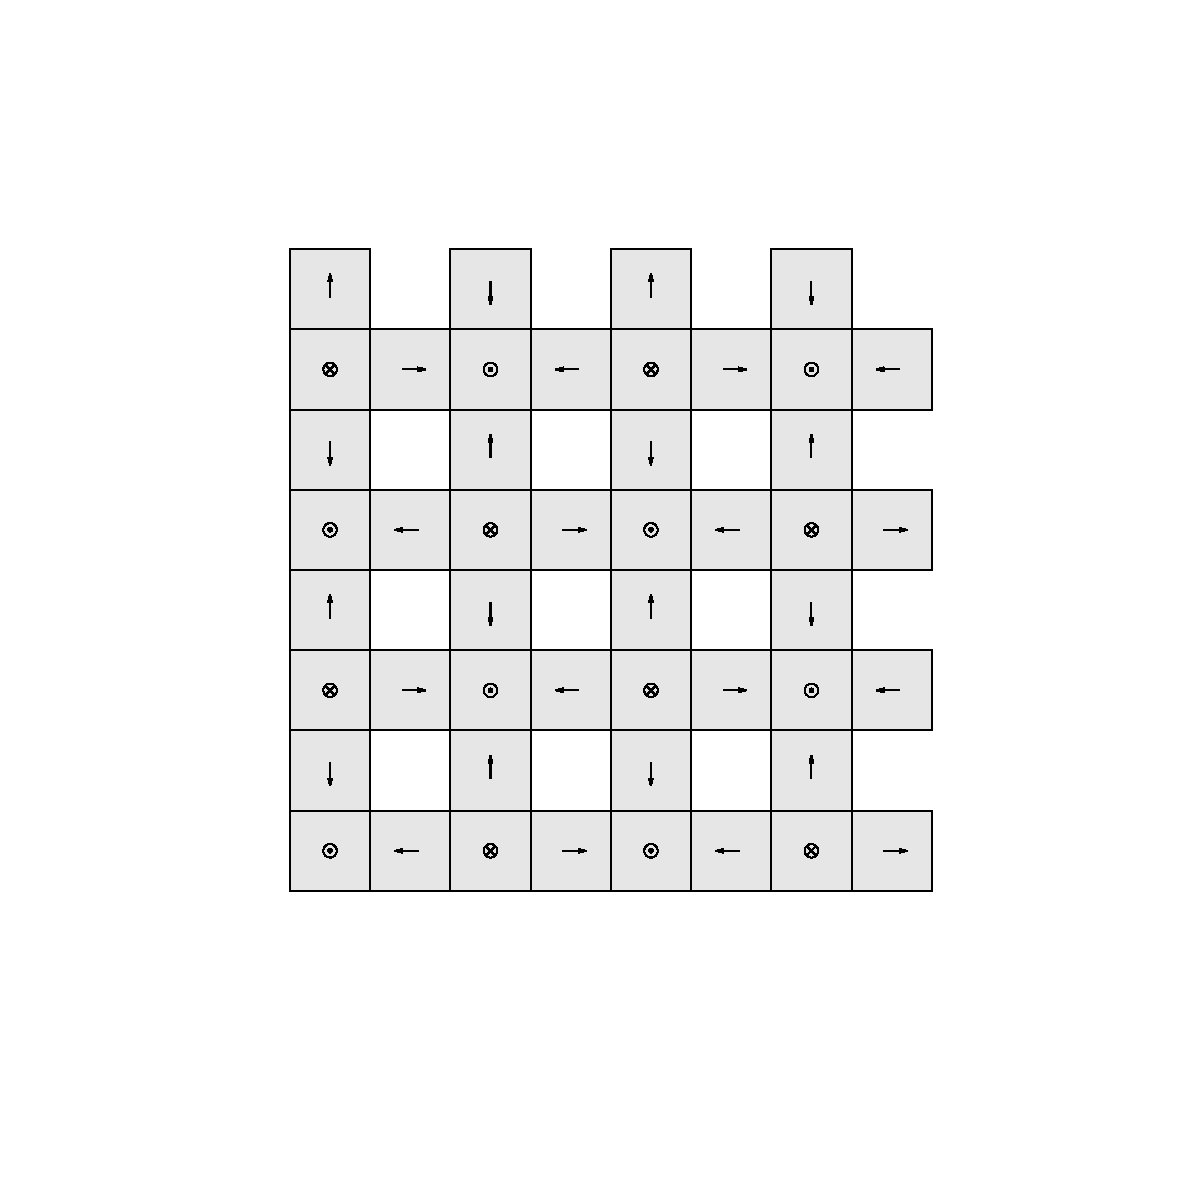
\includegraphics[width=\linewidth]{images/cuboidPlanarArraypdf.pdf}
        \vspace{-30mm}\subcaption{}
    \end{subfigure} \\
    \begin{subfigure}{\linewidth}
        \centering
        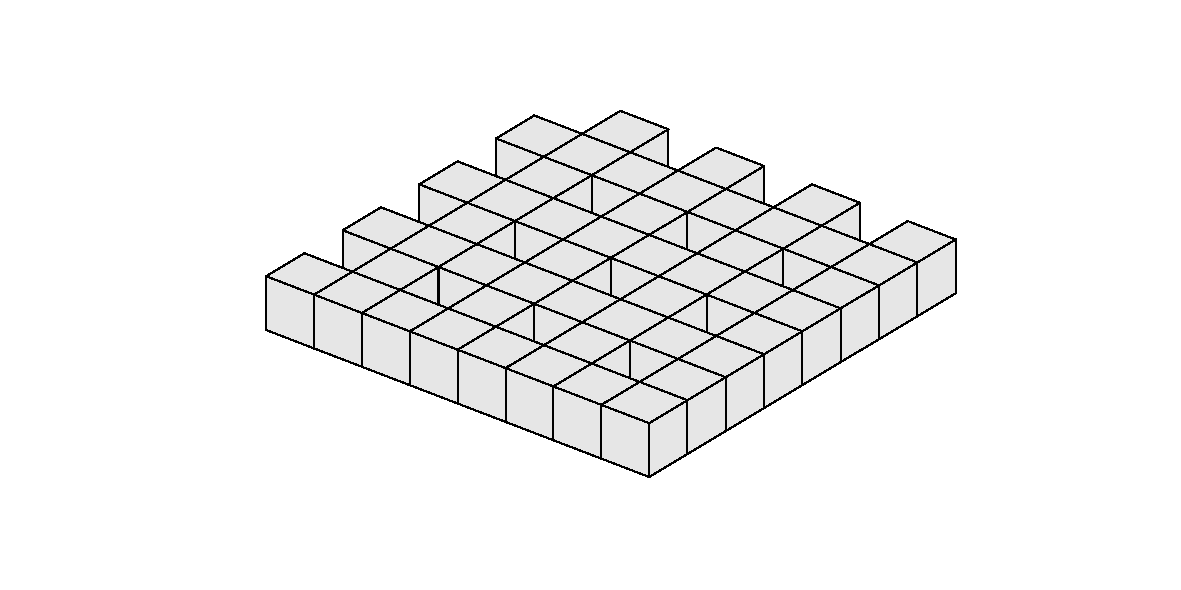
\includegraphics[width=\linewidth]{images/cuboidPlanarArrayAngledpdf.pdf}
        \vspace{-10mm}\subcaption{}
    \end{subfigure}
    \caption{Top view (a) and trimetric view (b) of a planar Halbach array created using cube permanent magnets. These are simple to produce, as only one configuration of magnet is required.}
    \label{fig:planarHalbachArray}
\end{figure}
However, to achieve the Halbach magnetisation pattern in two dimensions, some parts of the array must be empty, leading to unused space in the array. Many authors have attempted to optimise the planar array by modifying the relative size of the magnets, potentially reducing the unused space (Figure \ref{fig:planarHalbachArrayModifiedPoles}). Often, the magnets with magnetisations parallel to the plane are made smaller, while those with magnetisations orthogonal to the plane are made larger. In this way, the empty space in the array is reduced, while maintaining the Halbach magnetisation pattern.
\begin{figure}
    \centering
    \begin{subfigure}{\linewidth}
        \centering
        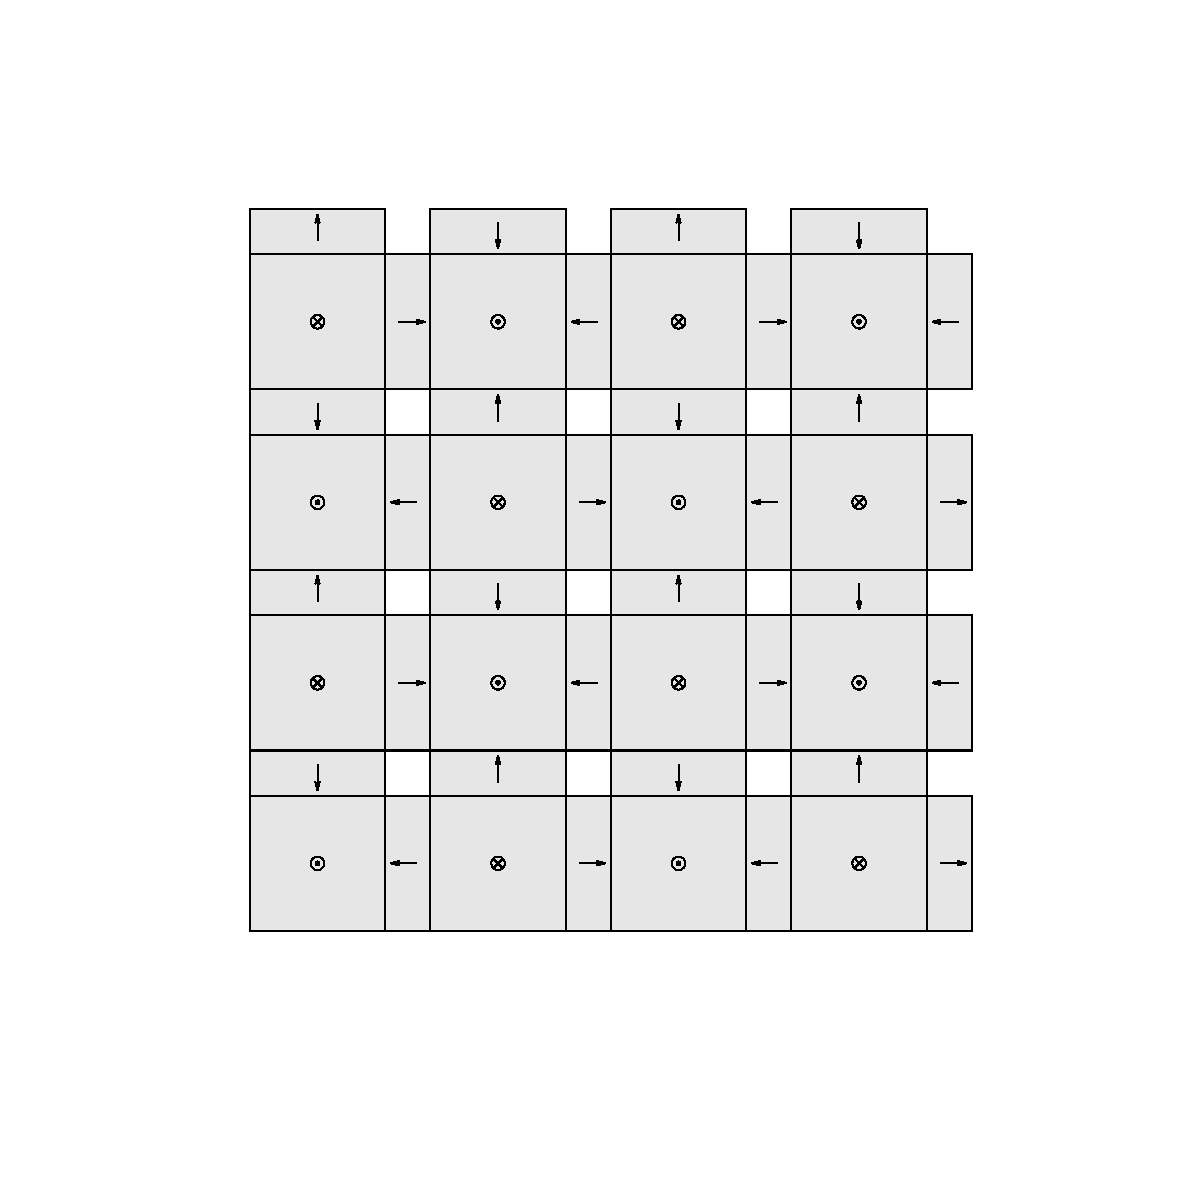
\includegraphics[width=\linewidth]{images/cuboidPlanarArrayReducedSpacepdf.pdf}
        \vspace{-25mm}\subcaption{}
    \end{subfigure} \\
    \begin{subfigure}{\linewidth}
        \centering
        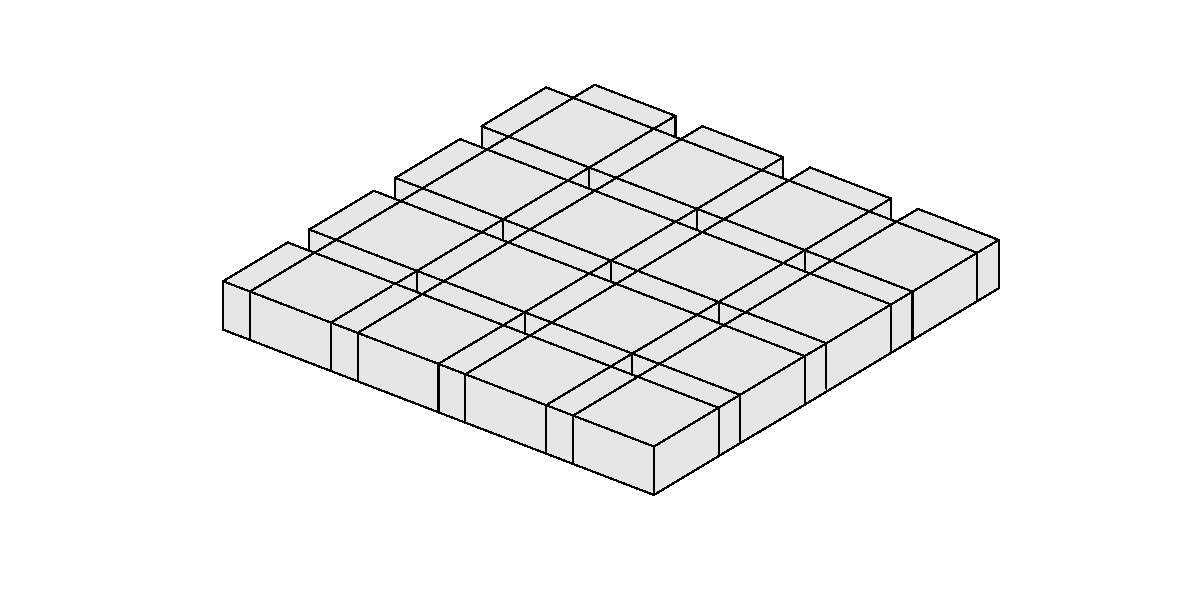
\includegraphics[width=\linewidth]{images/cuboidPlanarArrayReducedSpaceAngledpdf.pdf}
        \vspace{-10mm}\subcaption{}
    \end{subfigure}
    \caption{Top view (a) and trimetric view (b) of a planar Halbach array in which the magnets with magnetisations orthogonal to the array are made larger, thus reducing the empty space in the array.}
    \label{fig:planarHalbachArrayModifiedPoles}
\end{figure}
\begin{figure}
    \centering
    \begin{subfigure}{\linewidth}
        \centering
        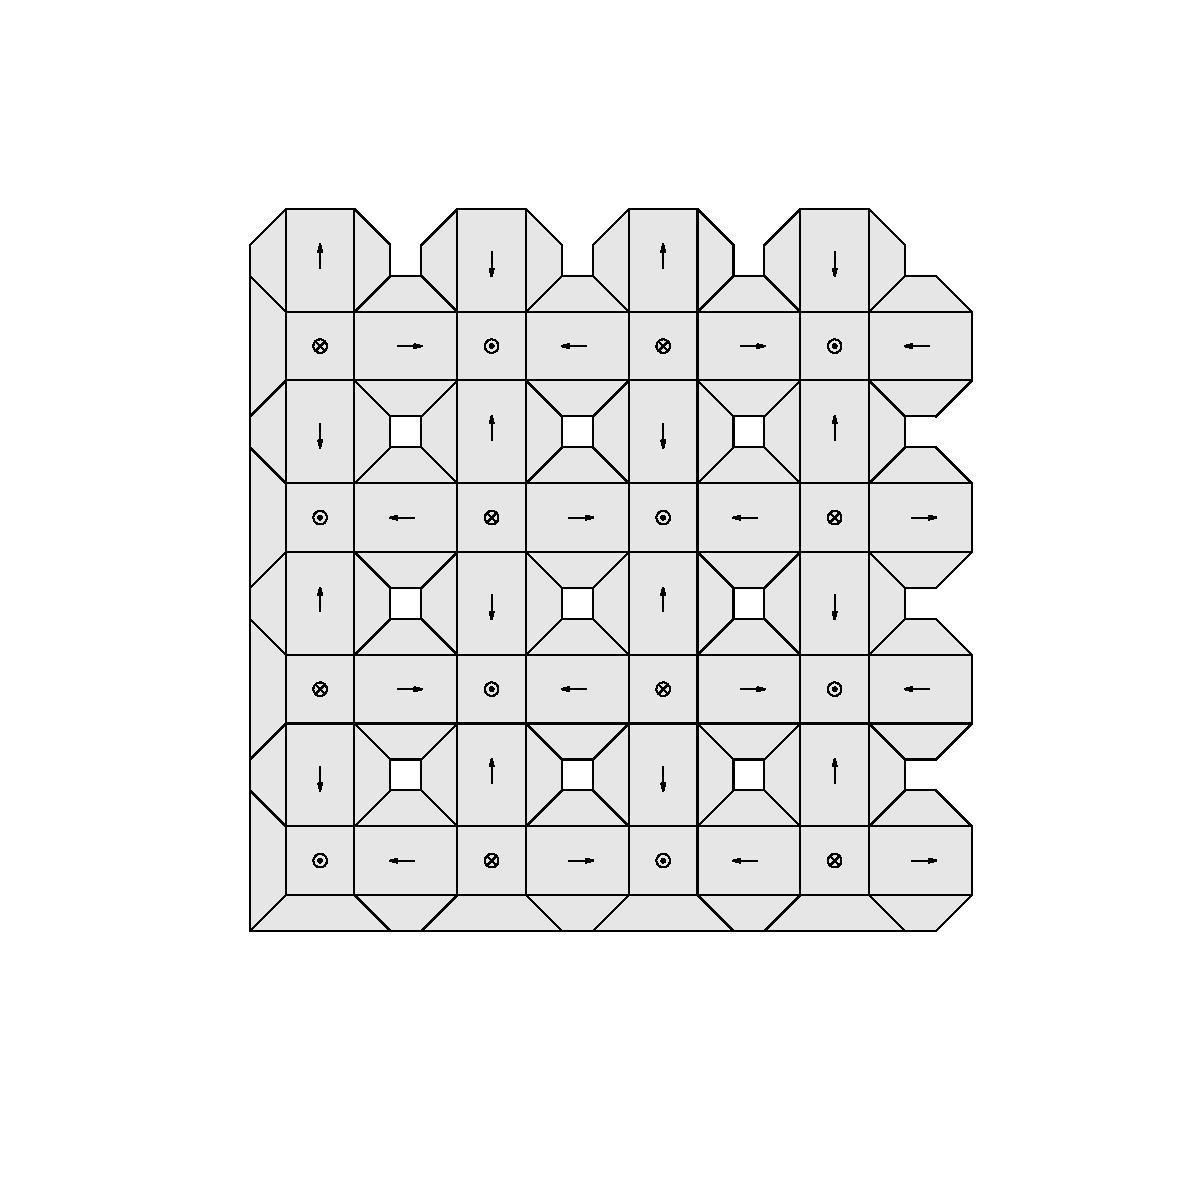
\includegraphics[width=\linewidth]{images/frustumPlanarArraypdf.pdf}
        \vspace{-25mm}\subcaption{}
    \end{subfigure} \\
    \begin{subfigure}{\linewidth}
        \centering
        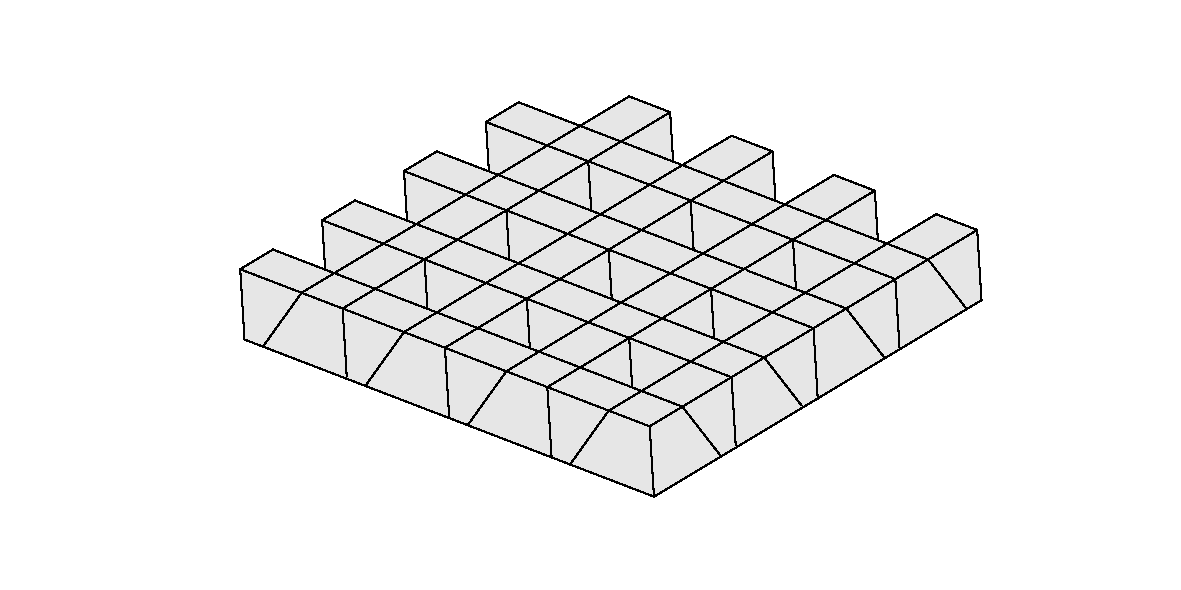
\includegraphics[width=\linewidth]{images/frustumPlanarArrayAngledpdf.pdf}
        \vspace{-10mm}\subcaption{}
    \end{subfigure}
    %\vspace{10cm}
    \caption{Top view (a) and trimetric view (b) of a planar Halbach array using pyramid and tetrahedral frustum magnets. This is the planar equivalent of the linear Halbach array with trapezial prismatic magnets shown in Figure \ref{fig:trapezoidalPrismaticHalbach}.}
    \label{fig:planarHalbachArrayPolyhedral}
\end{figure}

Further variations on planar Halbach geometry have been done, such as increasing the number of magnets for each repeating unit of the array. This leads to a more desirable field pattern with a larger field component orthogonal to the array while reducing the higher order harmonics of the field produced \cite{Min2010}. In addition, some authors have experimented with triangular prismatic magnets \cite{Cho2001,Cho2002} and frustum permanent magnets (Figure \ref{fig:planarHalbachArrayPolyhedral}) \cite{Peng2013,Janssen2009,Janssen2010a}, finding more desirable fields by varying and optimising magnet geometry.

\subsection{Permeability}
The effect of permeability leads to considerable difficulty in modelling permanent magnets. In essence, when a permanent magnet is exposed to a magnetic field, including its own, the magnetisation vector field is altered, with the effect being more significant for larger permeability. This is depicted in Figure \ref{fig:permeabilityOnMagnet}, with the top magnet being ideal, but the remanence magnetisation \(\mathbf{B}_r\) of the bottom becoming weaker due to its permeability, and some of the `magnetic charge' leaking to the sides of the magnet. The alteration of the magnetisation vector field leads to an altered field through the magnet, leading to further alteration of the magnetic vector field, and so on. In addition, the field through a magnet is not spatially constant; the field at one point inside a magnet is usually different from the field at another point. Thus, the magnetisation vector field is spatially varying, considerably increasing the modelling difficulty.
\begin{figure}
    \centering
    \begin{subfigure}{\textwidth}
        \centering
        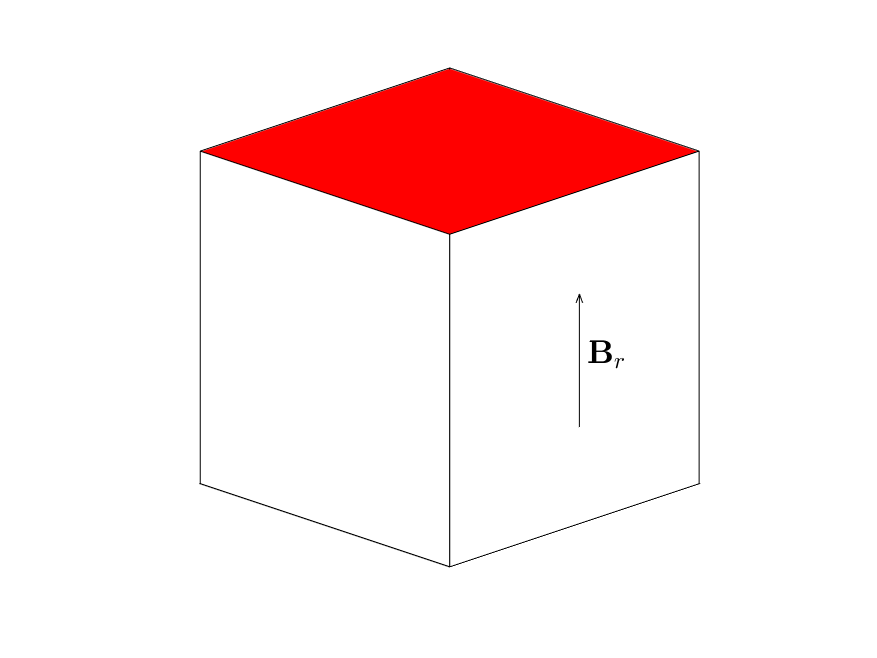
\includegraphics[width=0.65\linewidth]{p4/p4FIG1a}
        \caption{}\label{fig:introSingleMagnetIdealised}
    \end{subfigure}
    \begin{subfigure}{\textwidth}
        \centering
        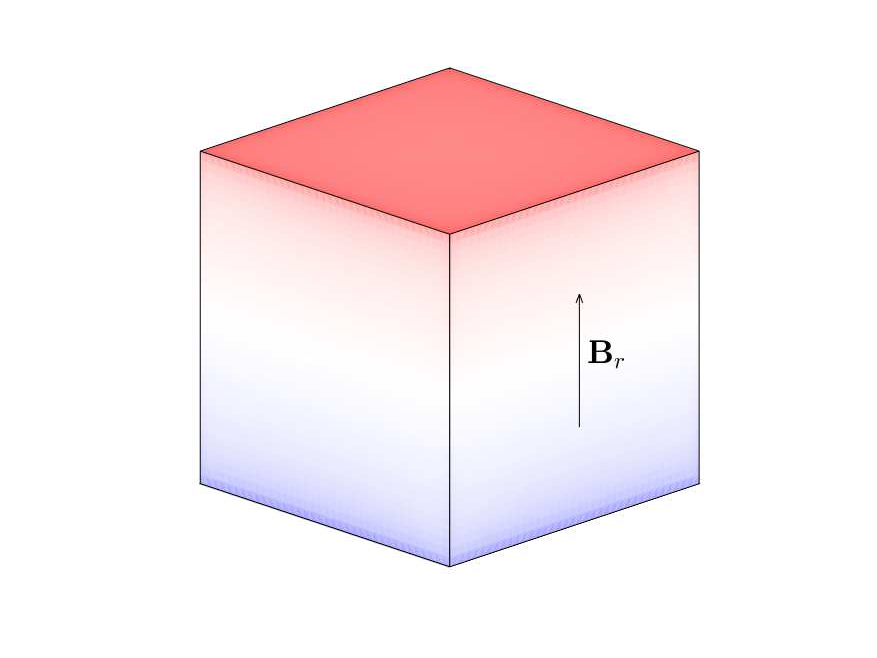
\includegraphics[width=0.65\linewidth]{p4/p4FIG1b}
        \caption{}\label{fig:introSingleMagnetNonideal}
    \end{subfigure}
    \caption{An ideal permanent magnet with relative permeability \(\mu_r = 1\) (\subref{fig:introSingleMagnetIdealised}), with the equivalent magnet but with permeability \(\mu_r = 3\) (\subref{fig:introSingleMagnetNonideal}). In the latter case, the surface charge is `leaking' onto the sides of the magnet under its own self-field, resulting in a weaker magnet overall.}
    \label{fig:permeabilityOnMagnet}
\end{figure}

Permanent magnets often have low permeabilities, with common values presented in Table \ref{tab:permeabilityClassificationTable}. Commonly used modern rare-earth neodymium magnets, for example, have a relative permeability of \(\mu_r \approx 1.05\). Therefore, the effect of permeability is small. Due to this, most research models permanent magnets with a relative permeability of unity, neglecting the effect of permeability as highlighted earlier in Section \ref{sec:geometrySolutions}. However, \textcite{Rovers2013} showed a nontrivial error when neglecting the permeability. Specifically, they modelled a cuboidal magnet with relative permeability \(\mu_r = 1.1\) and found an error of approximately 4\% in the magnetic field strength. They were able to mitigate this error by using the method of images to find an equivalent magnetisation vector. Similarly, \textcite{Kremers2013} found an expression for the equivalent magnetisation vector using the properties of permeability across the boundary of a magnet. It should be noted, however, that these studies do not consider spatially-varying magnetisation.

Other methods to model magnetic permeability involve subdividing a magnetic specimen into multiple surface or volume elements. For instance, \textcite{Forbes2021} subdivides a ring magnet into ring sector volumes, each being magnetically linear. This allows the modelling of nonlinear materials near saturation. Similarly, \textcite{Zhang2021} subdivides a cuboidal magnet into a large number of smaller cuboidal magnets and uses the magnetic surface charge method on each to calculate the total field. In contrast, \textcite{Casteren2014} subdivides the surface of a cuboidal magnet into small surface elements, each with their own surface charge density which is adjusted based on the field. However, each of these three methods requires iteration, since a change in the magnetisation vector or surface charge density changes the field, which requires further adjustment of the magnetisation vector or surface charge density, and so on, which can lead to considerable computation time.

\subsection{Literature summary}
Three-dimensional magnetostatic modelling of permanent magnets was first accomplished less than forty years ago. While much work has been done since, there are still many open problems, such as the force and torque between cuboidal magnets under general rotations, or the most optimal configuration for magnets in an array. Of particular interest to this thesis is the magnetic fields produced by polyhedral permanent magnets. While studies have derived equations for these fields, these equations are often complicated and computationally expensive, leading to slow force and torque calculations. Similarly, the magnetostatic modelling of permeability has been studied over the last decade, and solutions have been presented, but with a high computational cost. Therefore, this thesis aims to target the magnetostatic modelling of the magnetic fields, forces, and torques associated with permeable polyhedral permanent magnets.

\section{Thesis aims and scope}
Much of the current magnetic modelling literature is highly geometry-specific and requires ideal conditions. For example, the work by \textcite{Akoun1984} requires two magnets to be cuboidal with constant, uniform magnetisation vectors in the same direction, with both magnets having a relative permeability of unity. While other research is often more general than this, most is still rather specific. This thesis aims to further generalise magnetic modelling techniques by reducing the reliance on both magnet geometry and magnet permeability in a computationally efficient methodology.

The first primary objective of this thesis is to find new expressions for the magnetic field produced by general polyhedral permanent magnets, and to apply these to estimate forces and torques between these magnets. This is done by solving the magnetostatic charge model for generalised polyhedral magnets with unity relative permeability. The methodologies found are applicable to any magnet composed of flat faces, and magnets with curved faces may be approximated with polyhedra and the methodologies applied. The methodologies are also used to analyse planar arrays of magnets for use in a planar actuator.

The second objective of this thesis is to derive a method to model magnetically linear permeable materials of polyhedral geometry. This is based on the theory of permeability and uses the methods from the first objective to estimate the magnetic fields, forces, and torques produced by magnetically linear polyhedral magnetic materials.

Both objectives are undertaken with computation efficiency in mind. Vectorised code is used where possible, and mathematical expressions are simplified to avoid unnecessary computations. The equations and methodologies are implemented in interpreted MATLAB code. While compiled C++ code may be faster, MATLAB code provides far more flexibility and rapid prototyping of code due to the interpretive nature. While parallelised code can dramatically increase computation speed of large problems, the overhead associated with parallelisation may hurt the computation of small problems. As such, most code is non-parallelised, with the exception of the large optimisation problem in Chapter \ref{chap:paper3}.

In summary, achieving the main aims and objectives in this thesis will allow fast and accurate modelling of permanent magnets and other linear magnetic materials.

\section{Thesis format}
This thesis is presented in a \textit{Thesis by publication} format, with three articles (forming Chapters \ref{chap:paper1} to \ref{chap:paper3}) published, and one article (forming Chapter \ref{chap:paper4}) submitted. All articles have been submitted to high ranking journals in the magnetic modelling area of research.

\section{Thesis outline}
This thesis begins with a brief historical overview of the development of electromagnetism as a science, commencing with the first recordings of magnetism, and concluding with the discovery of quantum mechanics and electron spin.

Chapter \ref{chap:introduction} follows, detailing the mathematical background of magnetism and giving a review of current literature on magnetic modelling. This chapter outlines the current gaps in knowledge of the magnetic science, and summarises the main purpose of this thesis.

The substantive work of the thesis begins in Chapter \ref{chap:paper1}, which details a methodology to evaluate the magnetic field produced by a polyhedral magnet and estimate the force and torque between two polyhedral magnets. While this method is effective when calculating the magnetic field at a single point, it becomes less efficient when evaluating the field at many points. Therefore, a new method was found, presented in Chapter \ref{chap:paper2}, which presents solved field equations which are considerably more effective when calculating the field at many points. This is useful for force and torque evaluation, since a numeric surface integral requires the field evaluated at each surface element, with a larger number of field evaluations leading to a more accurate force and torque result.

Chapter \ref{chap:paper3} presents a case study on planar Halbach arrays by using the methodology described in Chapter \ref{chap:paper2}. This explores using pyramid and tetrahedral frustum permanent magnets rather than the more traditional cuboidal magnets in a planar array.

The work presented in Chapters \ref{chap:paper1} to \ref{chap:paper3} require a relative permeability of unity, limiting their use case in real magnetic systems. To alleviate this limitation, Chapter \ref{chap:paper4} investigates magnetic permeability and details a method for modelling permeable permanent magnets. This method attempts to alleviate the requirement for iteration by calculating the magnetic field only once and performing a matrix inversion. This considerably reduces computation time at the cost of computational memory.

Finaly, the thesis is concluded in Chapter \ref{chap:conclusion}, which summarises the thesis as a whole and outlines potential future work to follow this thesis.
\newpage
\section*{References}
\addcontentsline{toc}{section}{\protect\numberline{}References}
\printbibliography[heading=none]
\chapter{Magnetic field computation optimised for few points}\label{chap:paper1}
\fancyhead[LE]{\scshape Chapter\ \ref{chap:paper1}}
In general, the magnetic field produced by a permanent magnet is difficult to calculate, with the difficulty increasing considerably with complicated geometries. Polyhedral magnets have been explored in literature, but often the expressions are long and complicated, and limited work has been done on force and torque evaluation. This chapter presents the first of two methodologies for calculating the magnetic field produced by ideal polyhedral permanent magnets. Field equations are derived based on square root, logarithmic, and arctangent functions, leading to high computation speed. In addition, force and torque estimations are presented and validated using finite element analysis (with unity relative permeability) and past literature where available. As is discussed in Chapter \ref{chap:paper2}, this methodology is the more effective of the two when the field is to be computed at few (\(\leq 10\)) points in space.
%\subsection*{Statement of authorship}
\renewcommand{\arraystretch}{1.5}
\begin{tabular}{m{0.25\textwidth} m{0.67\textwidth}}
    \hline \hline Paper title & Analytic Magnetic Fields and Semi-Analytic Forces and Torques Due to General Polyhedral Permanent Magnets \\ \hline
    Publication status & Published \\ \hline
    Publication details & J. L. G. O’Connell, W. S. P. Robertson, and B. S. Cazzolato, ``Analytic Magnetic Fields and Semi-Analytic Forces and Torques Due to General Polyhedral Permanent Magnets,'' in IEEE Transactions on Magnetics, vol. 56, no. 1, Jan. 2020, doi: 10.1109/TMAG.2019.2942538. \\ \hline \hline
\end{tabular}

\vfill

\subsection*{Principal author}
\begin{tabular}{p{0.25\textwidth} m{0.67\textwidth}}
    \hline \hline Name & James O'Connell \\ \hline
    Contribution & \begin{itemize}
        \setlength\itemsep{-2mm}
        \item[-] Idea conceptualisation
        \item[-] Review of relevant literature
        \item[-] Performed all mathematical analysis, including derivation of solved field equations and estimated force and torque expressions
        \item[-] Implemented all algorithms and equations in MATLAB code, including considerable code testing and improvement to increase computation speed
        \item[-] Validation of methodology, including creation of finite element simulations and data analysis
        \item[-] Performed optimisation of magnet geometry to optimise field strength at a particular point in space
        \item[-] Wrote manuscript draft and created all figures
        \item[-] Finalisation of article
        \item[-] Preparation and submission for publication, including author correspondence
    \end{itemize} \\ \hline
    Percentage & 90\% \\ \hline
    Certification & This paper reports on original research conducted by the author during the period of Higher Degree by Research candidature and is not subject to any obligations or contractual agreements with a third party that would constrain its inclusion in this thesis. The author listed above is the primary author of this paper. \\ \hline
    Signature & \begin{tabular}{m{45mm} m{10mm} m{20mm}}
    \vspace{0.5mm}\includegraphics[width=0.3\textwidth]{jamesSignature.PNG} & Date: & 8 Dec 2021
    \end{tabular} \\ \hline
\end{tabular}

\vfill
    
\subsection*{Co-author contributions}
By signing this statement of authorship, each author certifies that:
\begin{enumerate}
    \item the candidate's stated contribution to the publication is accurate (as detailed above);
    \item permission is granted for the candidate to include the publication in the thesis; and
    \item the sum of all co-author contributions is equal to 100\% less the candidate's stated contribution.
\end{enumerate}
\begin{tabular}{m{0.25\textwidth} m{0.67\textwidth}}
    \hline \hline Name & Will Robertson \\ \hline
    Contribution & 5\% \\ \hline
    Signature & \vspace{2mm}\includegraphics[height=10mm]{willSig} \\  \hline
    Date & 16 Dec 2021 \\
    \hline \hline Name & Ben Cazzolato \\ \hline
    Contribution & 5\% \\ \hline
    Signature & \vspace{2mm} \includegraphics[height=10mm]{benSig} \\ \hline
    Date & 16 Dec 2021 \\
    \hline \hline \vfill
\end{tabular}
\renewcommand{\arraystretch}{1}
\newpage
%
\section*{\LARGE Analytic magnetic fields and semi-analytic forces and torques due to general polyhedral permanent magnets}
James L.G. O'Connell, William S.P. Robertson, and Benjamin S. Cazzolato
\section*{Abstract}\addcontentsline{toc}{section}{\protect\numberline{}Abstract}\label{sec:p1abstract}
This paper outlines an algorithm which analytically calculates the magnetic field produced by a general polyhedral permanent magnet with any number of faces and arbitrary face orientations, then uses the algorithm to \mbox{semi-analytically} calculate the force and torque on a second general polyhedral magnet. The algorithm is validated against both literature and finite element simulations using cuboids and dodecahedra. It is then used to model a basic two-magnet repulsive system, where it is shown that frustum magnets can produce a larger force per unit volume than cuboidal magnets. The shape of the frustums is optimised to maximise the force between them at a given separation distance, showing a considerable increase in force when compared to cuboidal magnets with the same volume. This paper shows that there is scope to improve performance of magnetic systems by using novel magnet shapes, and presents an algorithm which can be used for this optimisation process.
\section{Introduction}\label{sec:p1introduction}
Permanent magnets have many applications in magnetic resonance imaging, gearing, actuators, and motors \cite{Furlani2001}. Furthermore, they can be an essential component in wave energy harvesting \cite{Mann2010}, vibration isolation \cite{Robertson2009}, and many other applications. Due to their extensive use in a number of industries, it is important to understand the interactions between them, improving the design and optimisation process of electromagnetic systems.

Throughout recent decades, researchers have attempted to understand interactions between permanent magnets. \textcite{Akoun1984} started this trend by calculating the force between two parallel cuboidal permanent magnets with parallel magnetisation by finding the interaction energy between the magnets. \textcite{Janssen2010} used the same energy-based approach, but instead calculated the torque on one of the magnets. \textcite{Allag2009} extended the force and torque expressions to non-parallel magnetisations. \textcite{EngelHerbert2005} and \textcite{Ravaud2009} have calculated the magnetic field of cuboidal magnets rather than forces and torques. However, these studies are limited to cuboidal magnets and cannot be used for any other shapes.

A number of studies have examined ring and cylindrical magnets rather than cuboids. \textcite{Furlani1995} was able to semi-analytically calculate the field due to radially magnetised ring magnet sectors. Several papers by Ravaud et al.\ \cite{Ravaud2008,Ravaud2008a,Ravaud2009a} have found expressions for radially and axially magnetised ring magnets and sectors. Again, however, these studies are limited to ring magnets and cannot be used for other geometries.

To mitigate this geometrical limitation, some researchers have explored polyhedral permanent magnets, generalising the solution to any three dimensional shape with flat facets. Some authors such as \textcite{Soltner2010} and \textcite{Meessen2008} have approximated the magnetic field of a polyhedral magnet using assumptions such as the dipole model or discretisation of shapes into cuboids, but these are not always accurate. Other authors, however, have been more successful in solving for the exact magnetic field. \textcite{Janssen2010a} and \textcite{Rubeck2013} were able to find analytic expressions for the magnetic field of a polyhedral magnet by decomposing it into a collection of simple two-dimensional planar surfaces. \textcite{Meessen2008} and \textcite{Lee2004} studied trapezoidal magnets in a Halbach array using discretised magnets and magnets of infinite thickness respectively and found improvement in the maximum magnetic field strength over more traditional cuboidal Halbach arrays. However, there has been little work on the forces and torques due to polyhedral permanent magnets.

Several studies by \textcite{Beleggia2003,Beleggia2005}, \textcite{Beleggia2004}, and \textcite{DeGraef2009} examine magnetic nanoparticles with arbitrary shape. They found expressions for the demagnetisation tensor field, interaction energy, force, and torque using a Fourier space approach. However, for most shapes, these must be calculated numerically, limiting the accuracy and speed of the solution.

This paper outlines a semi-analytic method for calculating the magnetic fields, forces, and torques for polyhedral permanent magnets. First, an algorithm to analytically calculate the magnetic field is presented. This method is similar to the magnetic field calculation method given by \textcite{Rubeck2013} but requires evaluation of fewer terms by using general scalene triangles rather than right-angled triangles. Then, numeric integration is performed to find the force and torque on a second polyhedral magnet due to the field from the first. This work is validated using past literature and finite element simulations on the magnetic configuration presented by \textcite{Akoun1984}. To further validate the algorithm, finite element simulations are performed on two perpendicularly magnetised dodecahedral magnets, which are compared to the semi-analytic solutions from this method. Once validated, a configuration involving two pyramidal frustum magnets is presented, where it is shown that the frustums can produce a larger repulsive force per unit volume than cuboidal magnets. Finally, this algorithm is used to optimise the geometry of the frustums to maximise the force between them.
\section{Methodology}\label{sec:p1methodology}
This work uses the charge method outlined by \textcite{Furlani2001}, where a fictitious magnetic charge is distributed over the surface of each magnet, and assumes a relative permeability \(\mu_r\) of unity with constant uniform magnetisation \(\mathbf{M}\). Recent studies have detailed methods for including the effect of non-unity permeability in calculations of the magnetic field from permanent magnets \cite{Dam2016}. While out of the scope for the current work, such methods can also be applied to the results presented here.

In this method, polyhedral permanent magnets are decomposed into the polygonal facets that make up the surface of the polyhedron. Each polygonal facet has a fictitious magnetic charge distribution, which creates a magnetic field and thus induces forces and torques on other magnets.

In this work, two magnets are defined, magnet A and magnet B. The force and torque on magnet B is calculated due to the field produced by magnet A. An algorithm to analytically calculate the field due to magnet A is presented. Then, a mesh is applied to the surface of magnet B and the field due to magnet A is calculated at each mesh element. Finally, numeric integration is performed to find the force and torque on magnet B. These steps are outlined in more detail below.
\begin{figure*}
	\centering
	\begin{subfigure}{0.4\textwidth}
		\centering
		\tdplotsetmaincoords{70}{110}
		\tdplotsetrotatedcoords{0}{0}{0}
		\begin{tikzpicture}[scale = 0.45,tdplot_rotated_coords]
		
		\coordinate (p1b) at (0,1,5);
		\coordinate (p2b) at (0,3,5);
		\coordinate (p3b) at (0,6,3);
		\coordinate (p4b) at (0,6,-2);
		\coordinate (p5b) at (0,1,-2);
		\coordinate (p1f) at (5,1,5);
		\coordinate (p2f) at (5,3,5);
		\coordinate (p3f) at (5,6,3);
		\coordinate (p4f) at (5,6,-2);
		\coordinate (p5f) at (5,1,-2);
		
		\draw (p1b) -- (p2b) -- (p3b) -- (p4b);% -- (p5b) -- cycle;
		\draw[fill=black!10] (p1f) -- (p2f) -- (p3f) -- (p4f) -- (p5f) -- cycle;
		\draw (p1f) -- (p1b);
		\draw (p2f) -- (p2b);
		\draw (p3f) -- (p3b);
		\draw (p4f) -- (p4b);
		
		\draw[->,thick] (5,3.5,0.5) -- (5,3.5,2.5);
		\node (M1) at (5,4,1.5) {\textbf{M}};
		\end{tikzpicture}
		\caption{}
		\label{fig:p13dpolyhedron}
	\end{subfigure}
	
	\vspace{20pt}
	
	\begin{subfigure}{0.4\textwidth}
		\centering
		\begin{tikzpicture}[scale=0.45]
		\coordinate (origin) at (0,0);
		\coordinate (p5) at (1,5);
		\coordinate (p4) at (3,5);
		\coordinate (p3) at (6,3);
		\coordinate (p2) at (6,-2);
		\coordinate (p1) at (1,-2);
		
		\filldraw[fill = black!10] (p1) -- (p2) -- (p3) -- (p4) -- (p5) -- cycle;
		
		\draw[dashed] (origin) node {} -- (p1) node[circle,fill=white,draw,solid] {1};
		\draw[dashed] (origin) node {} -- (p2) node[circle,fill=white,draw,solid] {2};
		\draw[dashed] (origin) node {} -- (p3) node[circle,fill=white,draw,solid] {3};
		\draw[dashed] (origin) node {} -- (p4) node[circle,fill=white,draw,solid] {4};
		\draw[dashed] (origin) node {} -- (p5) node[circle,fill=white,draw,solid] {5};
		
		\node (x) at (7,0.3){\(x\)};
		\node (y) at (-0.3,6.5){\(y\)};
		
		\draw [<->] (-1,0) -- (7,0);
		\draw [<->] (0,-3.5) -- (0,6.5);
		\end{tikzpicture}
		\caption{}
		\label{fig:p1polygondecomposition}
	\end{subfigure}
	~
	\begin{subfigure}{0.4\textwidth}
		\centering
		\begin{tikzpicture}[scale=0.45]
		\coordinate (origin) at (0,0);
		\coordinate (p2) at (2,1);
		\coordinate (p1) at (2,6);
		
		\draw[solid] (p1) -- (origin) -- (p2) -- cycle;
		\path (p1) node[circle,fill=white,draw,solid] {2} -- (p2) node[circle,fill=white,draw,solid] {1};
		
		\draw[dashed] (0,0) -- (1,-2) -- (6,-2) -- cycle;
		\path (6,-2) node[circle,fill=white,draw,dashed] {2} -- (1,-2) node[circle,fill=white,draw,dashed] {1};
		
		\node (x) at (7,0.3){\(x\)};
		\node (y) at (-0.3,6.5){\(y\)};
		
		\draw [<->] (-1,0) -- (7,0);
		\draw [<->] (0,-3.5) -- (0,6.5);
		
		\draw[<-] (1.2,3) to [out=-30,in=70] (3,-1.0);
		\end{tikzpicture}
		\caption{}
		\label{fig:p1makingtriangles}
	\end{subfigure}
	\caption{A simple polyhedral permanent magnet, created by chamfering one edge of a cuboid (a). The magnet is magnetised vertically upward, as indicated by the arrow. Each facet is rotated such that it is parallel to the \(XY\)-plane and a line is drawn from the \(z\)-axis to each vertex (b), creating \(n\) triangles from the \(n\)-sided facet. Each triangle is rotated such that the edge joining the two vertices is parallel to the \(y\)-axis (c). The field of each rotated triangle is calculated then rotated back to the initial state. Each of these fields is added to give the total field of the facet. This process is then repeated for all other facets of the polyhedron to give the total field of the polyhedron.}
	\label{fig:p1decomposethepolygon}
\end{figure*}

\subsection{Calculation of the field due to magnet A}
The field due to magnet A is found using a similar method to \textcite{Rubeck2013}, but the equations are more efficient. Unlike the field equations presented by \textcite{Janssen2010}, all expressions and sub-expressions here are purely real. The magnetic field is found by first taking a polyhedral permanent magnet, such as that shown in Figure \ref{fig:p13dpolyhedron}\footnote{The magnet shown in Figure \ref{fig:p1decomposethepolygon} is a 5 unit (width) by 7 unit (height) by 5 unit (depth) cuboid, with a chamfer cutting the top face to a width of 2 units and one of the vertical faces to a height of 5 units.}, and decomposing it into its polygonal facets. Each facet is rotated about the \(x\)- and \(y\)-axes, making it parallel to the \(XY\)-plane, using the rotation matrix \(R_{xy}\), given by
\begin{equation}
R_{xy} = \begin{bmatrix}
\frac{n_z}{\sqrt{n_x^2+n_z^2}} & 0 & -\frac{n_x}{\sqrt{n_x^2+n_z^2}} \\
-\frac{n_xn_y}{\sqrt{n_x^2+n_z^2}} & \sqrt{n_x^2+n_z^2} & \frac{n_yn_z}{\sqrt{n_x^2+n_z^2}} \\
n_x & n_y & n_z
\end{bmatrix} \text{,}
\end{equation}
\noindent where \(\hat{\mathbf{n}} = \left[ n_x, n_y, n_z \right]\) is the outward-facing unit normal vector of each facet. Once parallel to the \(XY\)-plane, a line is drawn from the \(z\)-axis to each polygon vertex, as shown in Figure \ref{fig:p1polygondecomposition}, forming \(n\) triangles, where \(n\) is the number of sides of the polygon. It is important that the last triangle is defined from vertex \(n\) to vertex 1. This is because this algorithm calculates the field due to each triangle, which may include area not covered by the polygon. For example, the triangle between the \(z\)-axis, vertex 1, and vertex 5 of the polygon shown in Figure \ref{fig:p1polygondecomposition} is not part of the polygon, but the field of it is calculated from the first four triangles. The fifth triangle is defined from vertex 5 to vertex 1, effectively creating a triangle which subtracts the field due to this area outside the polygon.

After \(n\) triangles have been defined, each one is rotated so that the side joining the two vertices is parallel to the \(y\)-axis, shown in Figure \ref{fig:p1makingtriangles}. This is done using the rotation matrix
\begin{equation}
R_z = \begin{bmatrix}
-\frac{y_2-y_1}{\sqrt{\left( y_2-y_1 \right)^2 + \left( x_2-x_1 \right)^2}} & \frac{x_2-x_1}{\sqrt{\left( y_2-y_1 \right)^2 + \left( x_2-x_1 \right)^2}} & 0 \\
-\frac{x_2-x_1}{\sqrt{\left( y_2-y_1 \right)^2 + \left( x_2-x_1 \right)^2}} & -\frac{y_2-y_1}{\sqrt{\left( y_2-y_1 \right)^2 + \left( x_2-x_1 \right)^2}} & 0 \\
0 & 0 & 1
\end{bmatrix} \text{,}\\
\end{equation}
\noindent where \(x_1\), \(x_2\), \(y_1\), and \(y_2\) are the \(x\) and \(y\) coordinates of the two vertices not intersecting the \(z\)-axis before the triangle is rotated.

After rotation, the charge model outlined by \textcite{Furlani2001} can be used to solve for the magnetic field due to each triangle using the following expression.
\begin{eqnarray}\label{eqn:p1chargeB}
\mathbf{B} = -\frac{\mu_0}{4\pi} \int_{V} \left( \nabla \cdot \mathbf{M} \right) \frac{\mathbf{x} - \mathbf{x}'}{\left| \mathbf{x} - \mathbf{x}' \right|^3} \ dv' + \frac{\mu_0}{4\pi} \oint_{S} \left( \mathbf{M} \cdot \hat{\mathbf{n}} \right) \frac{\mathbf{x} - \mathbf{x}'}{\left| \mathbf{x} - \mathbf{x}' \right|^3} \ ds' \text{,}
\end{eqnarray}
\noindent where \(\mathbf{B}\) is the magnetic field, \(\mu_0\) is the magnetic permeability of free space, \(\mathbf{M}\) is the magnetisation vector, \(\mathbf{x}\) is the point of interest, \(\mathbf{x}'\) is a point on or inside the magnet, \(d{\mathrm{v}}'\) is a volume element of the magnet, and \(d{\mathrm{s}}'\) is a surface element of the magnet.

Assuming constant uniform magnetisation \(\mathbf{M}\), the first integral in Equation (\ref{eqn:p1chargeB}) disappears as \(\nabla \cdot \mathbf{M}=0\). The magnetic field due to each triangle can then be found by solving the second integral, giving
\begin{align}\label{eqn:p1trieqns}
    B_{x\Delta} &= \frac{\mu_0 \mathbf{M} \cdot \mathbf{\hat{n}}}{4\pi} \left( \frac{1}{2}\log\frac{\left( l_{az2}+y_2\right)\left(l_{az1}-y_1\right)}{\left(l_{az2}-y_2\right)\left(l_{az1}+y_1\right)} + \right. \nonumber \\
	& \quad \quad \quad \quad \quad \quad \quad \left. \frac{y_1}{2l_{a1}} \log \frac{l_{az1}+l_{a1}}{l_{az1}-l_{a1}} - \frac{y_2}{2l_{a2}} \log \frac{l_{az2}+l_{a2}}{l_{az2}-l_{a2}} \right) \nonumber \\
    & \quad \nonumber \\
	B_{y\Delta} &= \frac{\mu_0 \mathbf{M} \cdot \mathbf{\hat{n}}}{4\pi} \left( \frac{a}{2l_{a2}} \log \frac{l_{az2}+l_{a2}}{l_{az2}-l_{a2}} - \frac{a}{2l_{a1}} \log \frac{l_{az1}+l_{a1}}{l_{az1}-l_{a1}} \right) \\
    & \quad \nonumber \\
	B_{z\Delta} &= -\frac{\mu_0 \mathbf{M} \cdot \mathbf{\hat{n}}}{4\pi} \left( \text{sgn} \left( z' \right) \arctan \frac{ay_2-ay_1}{y_1y_2+a^2} + \right. \nonumber \\
	& \quad \quad \quad \quad \quad \quad \quad \left. \arctan \frac{az'y_1l_{az2}-az'y_2l_{az1}}{z'^2y_1y_2+a^2l_{az1}l_{az2}} \right)  \text{,} \nonumber
\end{align}
%\begin{subequations}
%	\begin{eqnarray}
%	B_{x\Delta} &=& \frac{\mu_0 \mathbf{M} \cdot \mathbf{\hat{n}}}{4\pi} \left( \frac{1}{2}\log\frac{\left( l_{az2}+y_2\right)\left(l_{az1}-y_1\right)}{\left(l_{az2}-y_2\right)\left(l_{az1}+y_1\right)} + \right. \nonumber \\
%	& & \left. \frac{y_1}{2l_{a1}} \log \frac{l_{az1}+l_{a1}}{l_{az1}-l_{a1}} - \frac{y_2}{2l_{a2}} \log \frac{l_{az2}+l_{a2}}{l_{az2}-l_{a2}} \right) \\
%	&&\nonumber\\
%	B_{y\Delta} &=& \frac{\mu_0 \mathbf{M} \cdot \mathbf{\hat{n}}}{4\pi} \left( \frac{a}{2l_{a2}} \log \frac{l_{az2}+l_{a2}}{l_{az2}-l_{a2}} - \right. \nonumber \\
%	& & \left. \frac{a}{2l_{a1}} \log \frac{l_{az1}+l_{a1}}{l_{az1}-l_{a1}} \right)  \\
%	&&\nonumber\\
%	B_{z\Delta} &=& -\frac{\mu_0 \mathbf{M} \cdot \mathbf{\hat{n}}}{4\pi} \left( \text{sgn} \left( z' \right) \arctan \frac{ay_2-ay_1}{y_1y_2+a^2} + \right. \nonumber \\
%	& & \left. \arctan \frac{az'y_1l_{az2}-az'y_2l_{az1}}{z'^2y_1y_2+a^2l_{az1}l_{az2}} \right)  \text{,}
%	\end{eqnarray}
%\end{subequations}
\noindent with
\begin{align*}
l_{a1} &= \sqrt{a^2+y_1^2} \nonumber \\
l_{a2} &= \sqrt{a^2+y_2^2} \nonumber \\
l_{az1} &= \sqrt{a^2+y_1^2+z'^2} \nonumber \\
l_{az2} &= \sqrt{a^2+y_2^2+z'^2} \nonumber \text{,}
\end{align*}
\noindent where \(\log()\) is the natural logarithm, \(\text{sgn}()\) is the sign function, \(\arctan()\) is the arctangent, and \(\left( 0,0,z' \right)\), \(\left( a,y_1,z' \right)\), and \(\left( a,y_2,z' \right)\) are the coordinates of the triangle vertices after rotation. This field can then be rotated back to the original position using the rotation matrix \(R_z^{-1}\). The field due to each triangle is summed, giving the field of the polygonal facet. Then, the field due to the polygonal facet is rotated back to the original position using the rotation matrix \(R_{xy}^{-1}\). The total field due to magnet A is then calculated by summing the field contribution of each polygonal facet. This field calculation gives the magnetic field at the origin, but the magnetic field at any point can be calculated using a coordinate translation such that the point of interest lies on the origin. The magnetic field calculation can be represented using Algorithm \ref{alg:p1alg1}.
\begin{algorithm}
	\caption{Calculate the magnetic field of a polyhedral permanent magnet}
	\begin{algorithmic}[1]
		\State Set \(\mathbf{B} = [0,0,0]^\textsf{T}\).
		\For {each \(n\)-sided facet of the polyhedron}
		\State \parbox[t]{\dimexpr\linewidth-\leftmargin-\labelsep-\labelwidth}{Define the vertices in an anticlockwise order when looking at the polyhedron from the outside.}\newline
		\State \parbox[t]{\dimexpr\linewidth-\leftmargin-\labelsep-\labelwidth}{Store these in a \(3\times n\) matrix \(P\) such that each column represents a vertex.}\newline
		\State \parbox[t]{\dimexpr\linewidth-\leftmargin-\labelsep-\labelwidth}{Copy the first column of \(P\) and add it as the \(\left(n+1\right)\)th column.}\newline
		\State \parbox[t]{\dimexpr\linewidth-\leftmargin-\labelsep-\labelwidth}{Evaluate the matrix \(R_{xy}\) and create a new matrix \(P_{xy}\) given by \(P_{xy} = R_{xy}P\).}\newline
		\For {\(j=1,\dots,n\)}
		\State \parbox[t]{\dimexpr\linewidth-\leftmargin-\labelsep-\labelwidth}{Using the \(j\)th and \(\left(j+1\right)\)th columns of \(P_{xy}\), calculate \(R_z\). Create \(P_z\) given by \(P_z = R_zP_{xy}\).}\newline
		\State \parbox[t]{\dimexpr\linewidth-\leftmargin-\labelsep-\labelwidth}{Evaluate \(\textbf{B}_\Delta\) using the points from \(P_z\) and Equation (\ref{eqn:p1trieqns}).}\newline
		\State \label{alg:p1enum2}Add the value of \(\left(R_{xy}^{-1}R_z^{-1}\textbf{B}_\Delta\right)\) to \(\mathbf{B}\).
		\EndFor
		\EndFor
		\State The field at the origin is now equal to \(\mathbf{B}\).
	\end{algorithmic}\label{alg:p1alg1}
\end{algorithm}

Algorithm \ref{alg:p1alg1} was implemented on the three-dimensional polyhedral magnet shown in Figure \ref{fig:p1decomposethepolygon}. Flux lines were drawn on the plane of symmetry to give a visual representation of the magnetic field, and are shown in Figure \ref{fig:p1fluxlines}.
\begin{figure}
	\centering
	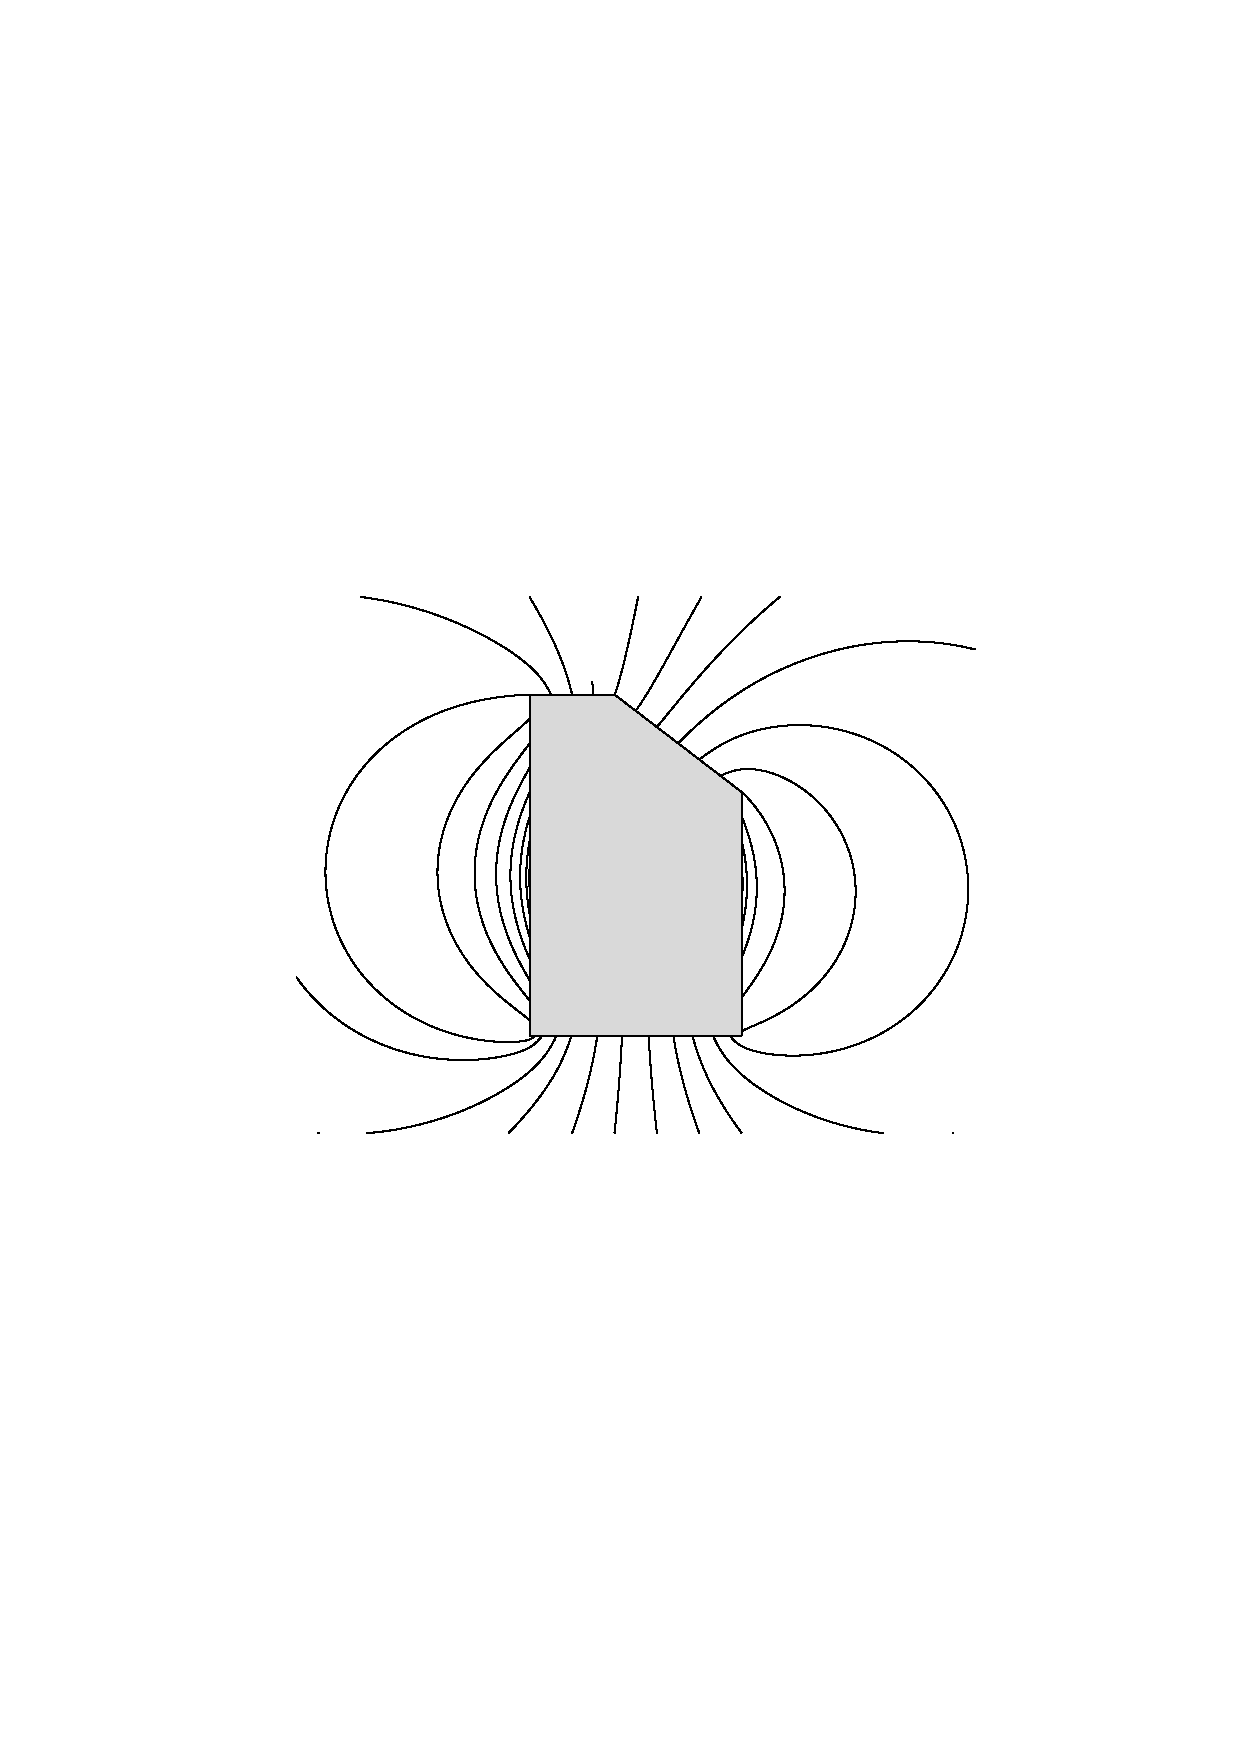
\includegraphics[trim = 3cm 10cm 3cm 10cm,width=0.8\linewidth]{p1/p1FIG2}
	\caption{The magnetic flux lines of the polyhedral magnet shown in Figure \ref{fig:p1decomposethepolygon}. The flux lines travel from the north pole (top) of the magnet to the south pole (bottom) of the magnet. The flux lines behave similarly to that of a cuboidal magnet in most regions due to the magnet being almost cuboidal. However, in the top right region, the flux lines differ from those of a cuboidal magnet due to the chamfer.}
	\label{fig:p1fluxlines}
\end{figure}

\subsection{Force and torque on magnet B}
The force and torque on magnet B is found using numeric integration of the magnetic field due to magnet A over the surface of magnet B, as described by \textcite{Furlani2001}. This is done by numerically solving the integrals
\begin{subequations}
    \begin{eqnarray}
	\mathbf{F}_\text{B} &=& \oint_{S_\text{B}} \left( \mathbf{M}_\text{B} \cdot \mathbf{\hat{n}}_\text{B} \right) \mathbf{B}_\text{A}\  ds_\text{B} \text{,} \\
	\mathbf{T}_\text{B} &=& \oint_{S_\text{B}} \left( \mathbf{M}_\text{B} \cdot \mathbf{\hat{n}}_\text{B} \right) \left( \mathbf{r}_\text{B} \times \mathbf{B}_\text{A} \right)\ ds_\text{B} \text{,}
	\end{eqnarray}
\end{subequations}
\noindent where \({S_\mathrm{B}}\) is the surface of magnet B, \({\mathbf{M}_\mathrm{B}}\) is the magnetisation vector of magnet B, \({\mathbf{\hat{n}}_\mathrm{B}}\) is the outward-facing normal vector of the surface of magnet B, \({\mathbf{B}_\mathrm{A}}\) is the field due to magnet A, and \({\mathbf{r}_\mathrm{B}}\) is the vector from the point of rotation of magnet B to the surface of magnet B.

To solve these expressions, a mesh is defined on the surface of magnet B. This mesh must be defined such that the field due to magnet A is relatively constant over each element. The field due to magnet A is evaluated at the centre of each mesh element using Algorithm \ref{alg:p1alg1}. The force and torque on magnet B can be found by numerically integrating the field at each element with area \(A_i\), as shown in Equation (\ref{eqn:p1numericforcetorque}), where \(\mathbf{b}_i\) is the field due to magnet A at the centre of each mesh element.
\begin{subequations}
	\label{eqn:p1numericforcetorque}
	\begin{eqnarray}
	\mathbf{F}_\text{B} &=& \sum_i \left( \mathbf{M}_\text{B} \cdot \mathbf{\hat{n}}_\text{B} \right) {\mathbf{b}_i A_i} \text{,} \\
	\mathbf{T}_\text{B} &=& \sum_i \left( \mathbf{M}_\text{B} \cdot \mathbf{\hat{n}}_\text{B} \right) \left( {\mathbf{r}_i \times \mathbf{b}_i} \right) A_i \text{.}
	\end{eqnarray}
\end{subequations}

This process can be represented programmatically using Algorithm \ref{alg:p1alg2}.
\begin{algorithm}
	\caption{Calculate the force and torque on a polyhedral permanent magnet}
	\begin{algorithmic}[1]
		\State Apply a mesh to the surface of magnet B.
		\For {each mesh element \(i\) on the surface of magnet B}
		\State \parbox[t]{\dimexpr\linewidth-\leftmargin-\labelsep-\labelwidth}{Translate the entire system so the centre of the element lies on the origin.}\newline
		\State \parbox[t]{\dimexpr\linewidth-\leftmargin-\labelsep-\labelwidth}{Calculate the magnetic field strength from magnet A using Algorithm \ref{alg:p1alg1}.}\newline
		\State \parbox[t]{\dimexpr\linewidth-\leftmargin-\labelsep-\labelwidth}{Calculate the cross product of the torque moment arm and the magnetic field strength \(\mathbf{r}\times\mathbf{b}\).}\newline
		\State Calculate the quantity \(\mathbf{M}\cdot\hat{\mathbf{n}}\) for the element.
		\State \parbox[t]{\dimexpr\linewidth-\leftmargin-\labelsep-\labelwidth+4mm}{Set \(\mathbf{f}_i=\left(\mathbf{M}\cdot\hat{\mathbf{n}}\right)\mathbf{b}A_i\) and \(\mathbf{\tau}_i=\left(\mathbf{M}\cdot\hat{\mathbf{n}}\right)\left(\mathbf{r}\times\mathbf{b}\right)A_i\) where \(A_i\) is the area of the element.}\newline
		\EndFor
		\State {Set \(\mathbf{F} = \sum_i\mathbf{f}_i\) and \(\mathbf{T} = \sum_i\mathbf{\tau}_i\).}
		\State The force and torque on magnet B are given by \(\mathbf{F}\) and \(\mathbf{T}\) respectively.
	\end{algorithmic}\label{alg:p1alg2}
\end{algorithm}

Thus the exact magnetic field due to a polyhedral permanent magnet has been analytically calculated, and the force and torque on a second polyhedral magnet has been numerically calculated using the analytic field solution.
\section{Validation}\label{sec:p1validation}
The field, force, and torque solutions outlined in Section \ref{sec:p1methodology} have been verified using both previous literature and finite element simulations. Firstly, the configuration used by \textcite{Akoun1984}\footnote{\textcite{Akoun1984} used two cuboidal magnets, each of dimensions 20mm by 12mm by 6mm with a vertical gap of 2mm between them.} was considered (Figure \ref{fig:p1akounyonnet}). Here, the force on magnet B is measured as it moves a distance \(d\) in the \(x\)-direction while magnet A remains fixed. Both magnets have parallel magnetisation vectors in the \(z\)-direction with a value of 0.38 Tesla. The resulting force and torque depends not only on magnetisation, but also on the geometry of the magnets.
\begin{figure*}
	\centering
	\begin{subfigure}{0.4\textwidth}
		\centering
		\tdplotsetmaincoords{70}{130}
		\begin{tikzpicture}[scale=0.2,tdplot_main_coords]
		\coordinate(b1) at (10,-6,3);
		\coordinate(b2) at (10,6,3);
		\coordinate(b3) at (-10,6,3);
		\coordinate(b4) at (-10,-6,3);
		\coordinate(b5) at (10,-6,-3);
		\coordinate(b6) at (10,6,-3);
		\coordinate(b7) at (-10,6,-3);
		
		\draw (b1) -- (b2) -- (b3) -- (b4) -- cycle;
		\draw (b5) -- (b6) -- (b7);
		\draw (b1) -- (b5);
		\draw (b2) -- (b6);
		\draw (b3) -- (b7);
		
		\coordinate(t1) at (2,-14,11);
		\coordinate(t2) at (2,6,11);
		\coordinate(t3) at (-10,6,11);
		\coordinate(t4) at (-10,-14,11);
		\coordinate(t5) at (2,-14,5);
		\coordinate(t6) at (2,6,5);
		\coordinate(t7) at (-10,6,5);
		
		\draw[fill=white] (t1) -- (t2) -- (t6) -- (t5);
		\draw[fill=white] (t2) -- (t3) -- (t7) -- (t6);
		\draw (t5) -- (t1) -- (t4) -- (t3);
		
		\coordinate(midpt) at (2,-4,8);
		\coordinate(end) at (12,-4,8);
		
		\draw[->,dashed] (midpt) -- (end);
		
		\node(d) at (14.5,-3,8.5) {\textit{d}};
		\node(A) at (0,6,0) {\text{A}};
		\node(B) at (-4,6,8) {\text{B}};
		\end{tikzpicture}
		\caption{}
	\end{subfigure}
	~ \hspace{1cm}
	\begin{subfigure}{0.4\textwidth}
		\centering
		\tdplotsetmaincoords{90}{180}
		\begin{tikzpicture}[scale=0.2,tdplot_main_coords]
		\coordinate(b1) at (10,-6,3);
		\coordinate(b2) at (10,6,3);
		\coordinate(b3) at (-10,6,3);
		\coordinate(b4) at (-10,-6,3);
		\coordinate(b5) at (10,-6,-3);
		\coordinate(b6) at (10,6,-3);
		\coordinate(b7) at (-10,6,-3);
		
		\draw (b1) -- (b2) -- (b3) -- (b4) -- cycle;
		\draw (b5) -- (b6) -- (b7);
		\draw (b1) -- (b5);
		\draw (b2) -- (b6);
		\draw (b3) -- (b7);
		
		\coordinate(t1) at (2,-14,11);
		\coordinate(t2) at (2,6,11);
		\coordinate(t3) at (-10,6,11);
		\coordinate(t4) at (-10,-14,11);
		\coordinate(t5) at (2,-14,5);
		\coordinate(t6) at (2,6,5);
		\coordinate(t7) at (-10,6,5);
		
		\draw[fill=white] (t1) -- (t2) -- (t6) -- (t5);
		\draw[fill=white] (t2) -- (t3) -- (t7) -- (t6);
		\draw (t5) -- (t1) -- (t4) -- (t3);
		
		\coordinate(midpt) at (2,-4,8);
		\coordinate(end) at (6,-4,8);
		
		\draw[->,dashed] (midpt) -- (end);
		\node(d) at (7,-3,8) {\textit{d}};
		
		\draw[->,thick] (-4,0,6.5) -- (-4,0,9.5);
		\node (M1) at (-2.5,0,8) {\textbf{M}};
		\draw[->,thick] (0,0,-1.5) -- (0,0,1.5);
		\node (M2) at (1.5,0,0) {\textbf{M}};
		
		\node (A) at (-8,6,0) {\text{A}};
		\node(B) at (-8,6,8) {\text{B}};
		
		\draw [->] (-15,-4,-3) -- (-12,-4,-3);
		\draw [->] (-15,-4,-3) -- (-15,-4,0);
		\node (x) at (-11,-4,-3) {\(x\)};
		\node (z) at (-15,-4,1) {\(z\)};
		\end{tikzpicture}
		\caption{}
	\end{subfigure}
	\caption{The geometry used in Akoun and Yonnet's work in 1984 \cite{Akoun1984} with both magnets having parallel magnetisation in the \(z\)-direction. Magnet B moves a distance \(d\) along the top of magnet A.}
	\label{fig:p1akounyonnet}
\end{figure*}

Algorithms \ref{alg:p1alg1} and \ref{alg:p1alg2} were implemented in Matlab R2017b (MathWorks, Inc., Natick, MA, USA), with a basic meshing process using triangular elements. The mesh was created by repeatedly bisecting each triangle edge and joining the three bisection points, converting the triangle into four smaller triangles, until all triangles in the mesh had area less than a threshold value. Algorithms \ref{alg:p1alg1} and \ref{alg:p1alg2} were applied to Akoun and Yonnet's geometry \cite{Akoun1984} to calculate force and torque values for varying displacement. The finite element package Maxwell3D in ANSYS Electronics Desktop 2018.0 (ANSYS, Inc., Berkeley, CA, USA) was used with adaptive meshing to obtain finite element solutions for the force and torque in this configuration. Additionally, the force solutions presented by \textcite{Akoun1984} and torque solutions presented by \textcite{Janssen2010a} were calculated using Matlab code from Robertson \cite{Robertson2013,Robertson}, with the torque being evaluated about the centre of magnet B. These results were compared to those obtained with Algorithms \ref{alg:p1alg1} and \ref{alg:p1alg2} as well as finite element simulations.
\begin{figure*}
	\centering
	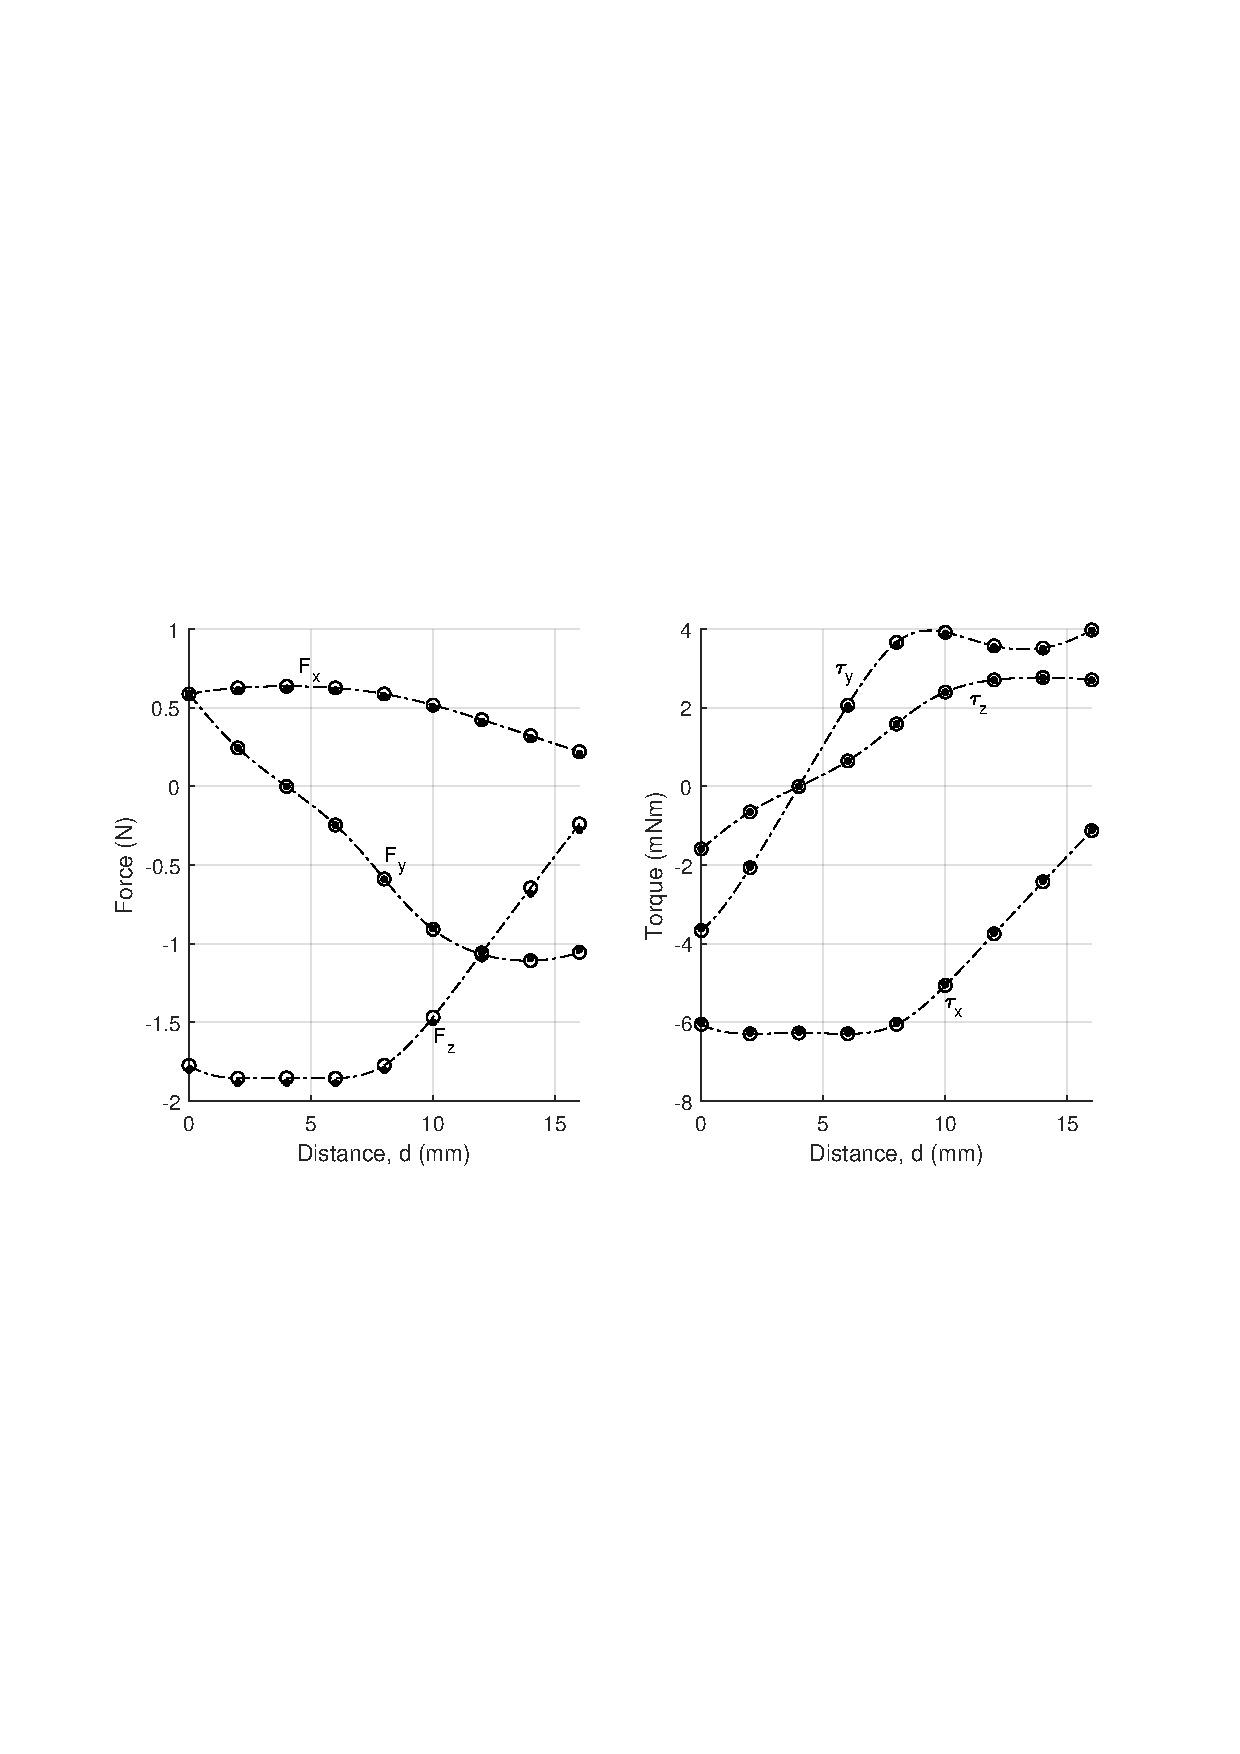
\includegraphics[trim = 3cm 9cm 3cm 9cm,width=0.9\linewidth]{p1/p1FIG4}
	\caption{Forces and torques on magnet B shown in Figure \ref{fig:p1akounyonnet} as it moves a distance \(d\) along the top of the magnet A. The dashed lines represent the results calculated from Algorithms \ref{alg:p1alg1} and \ref{alg:p1alg2}, with circles representing analytic solutions \cite{Akoun1984,Janssen2010a} and dots representing solutions obtained from a finite element simulation (Maxwell3D, ANSYS Electronics Desktop 2018.0). The values obtained with Algorithms \ref{alg:p1alg1} and \ref{alg:p1alg2} are in excellent agreement with the other two methods, especially the analytic solutions, indicating this work produces correct results for cuboidal magnets.}
	\label{fig:p1cuboidcase}
\end{figure*}

The three sets of results are shown in Figure \ref{fig:p1cuboidcase}. The forces and torques obtained from Algorithms \ref{alg:p1alg1} and \ref{alg:p1alg2} align with both the values from the finite element simulation and from the analytic solution, validating the algorithms for simple cuboidal magnets with parallel magnetisation. However, this test does not consider non-cuboidal magnets or non-parallel magnetisation and these must be considered for further validation.

Algorithms \ref{alg:p1alg1} and \ref{alg:p1alg2} were significantly faster than the finite element simulations when implemented in Matlab R2017b (MathWorks, Inc., Natick, MA, USA) on a workstation PC with an Intel Xeon E3-1240 v5 (3.50GHz) with 4 cores. Algorithms \ref{alg:p1alg1} and \ref{alg:p1alg2} completed each force calculation in approximately 0.65 seconds using 3072 triangular elements on the surface of magnet B, while the finite element simulations took a minimum of 30-40 seconds using an adaptive setup with a percent error of 1\% and approximately 17000 tetrahedral elements. Additionally, Algorithms \ref{alg:p1alg1} and \ref{alg:p1alg2} were considerably more accurate, achieving a maximum force error of 4.3 milliNewtons and a maximum torque error of 0.03 milliNewton-metres when compared to the analytic solutions, while the finite element solutions gave a maximum force error of 37 milliNewtons and a maximum torque error of 0.14 milliNewton-metres.

To validate Algorithms \ref{alg:p1alg1} and \ref{alg:p1alg2} for a more general case, two dodecahedral magnets were considered (Figure~\ref{fig:p1dodecahedra}). Both magnets are regular dodecahedra with edge lengths of 20mm and volumes of 61305mm\(^3\). Magnet B has magnetisation in the \(x\)-direction and may move vertically, while magnet A has magnetisation in the \(z\)-direction and is fixed. Both magnets have a unit magnetisation strength \(\mathbf{M}\), i.e. 1 Tesla. The \(x\)-force and \(y\)-torque on magnet B are calculated, with the torque calculated about its centre. The \(y\)- and \(z\)-forces, as well as the \(x\)- and \(z\)-torques are almost zero and thus neglected. The magnetic configuration was input into Algorithms \ref{alg:p1alg1} and \ref{alg:p1alg2} as well as a  three-dimensional finite element simulation, with the results shown in Figure \ref{fig:p1dodecahedraresults}\footnote{Due to the numeric nature of the force and torque calculations, accuracy is reduced when magnets are extremely close and an insufficient surface mesh density is used. As such, the magnets were limited to a minimum separation of 1mm.}. Due to symmetry, the forces in the \(y\) and \(z\) directions, as well as the torques about the \(x\) and \(z\) axes are extremely small and therefore not plotted in the figure.
\begin{figure*}
	\centering
	\begin{subfigure}{0.49\textwidth}
		\centering
		\tdplotsetmaincoords{70}{110}
		\begin{tikzpicture}[scale=50,tdplot_main_coords]
		\coordinate(p1t) at (0.026180,0.008506,0.005258);
		\coordinate(p2t) at (0.016181,-0.005257,-0.022270);
		\coordinate(p3t) at (0.009999,-0.013765,0.022270);
		\coordinate(p4t) at (0.000000,-0.027527,-0.005258);
		\coordinate(p5t) at (-0.000000,0.027527,0.005258);
		\coordinate(p6t) at (-0.009999,0.013765,-0.022270);
		\coordinate(p7t) at (-0.016181,0.005257,0.022270);
		\coordinate(p8t) at (-0.026180,-0.008506,-0.005258);
		\coordinate(p9t) at (0.016180,0.022271,-0.005256);
		\coordinate(p10t) at (0.010001,0.013765,-0.022270);
		\coordinate(p11t) at (-0.010001,-0.013765,0.022270);
		\coordinate(p12t) at (-0.016180,-0.022271,0.005256);
		\coordinate(p13t) at (0.016180,0.005257,0.022271);
		\coordinate(p14t) at (0.000001,-0.017012,-0.022271);
		\coordinate(p15t) at (-0.000001,0.017012,0.022271);
		\coordinate(p16t) at (-0.016180,-0.005257,-0.022271);
		\coordinate(p17t) at (0.026180,-0.008506,-0.005257);
		\coordinate(p18t) at (0.016180,-0.022271,0.005257);
		\coordinate(p19t) at (-0.016180,0.022271,-0.005257);
		\coordinate(p20t) at (-0.026180,0.008506,0.005257);
		
		\coordinate(p1b) at (0.016180,0.022270,-0.049242);
		\coordinate(p2b) at (0.016180,0.005258,-0.076770);
		\coordinate(p3b) at (0.016180,-0.005258,-0.032230);
		\coordinate(p4b) at (0.016180,-0.022270,-0.059758);
		\coordinate(p5b) at (-0.016180,0.022270,-0.049242);
		\coordinate(p6b) at (-0.016180,0.005258,-0.076770);
		\coordinate(p7b) at (-0.016180,-0.005258,-0.032230);
		\coordinate(p8b) at (-0.016180,-0.022270,-0.059758);
		\coordinate(p9b) at (0.000000,0.027528,-0.059756);
		\coordinate(p10b) at (0.000000,0.017014,-0.076770);
		\coordinate(p11b) at (0.000000,-0.017014,-0.032230);
		\coordinate(p12b) at (0.000000,-0.027528,-0.049244);
		\coordinate(p13b) at (0.010000,0.013763,-0.032229);
		\coordinate(p14b) at (0.010000,-0.013763,-0.076771);
		\coordinate(p15b) at (-0.010000,0.013763,-0.032229);
		\coordinate(p16b) at (-0.010000,-0.013763,-0.076771);
		\coordinate(p17b) at (0.026180,0.008507,-0.059757);
		\coordinate(p18b) at (0.026180,-0.008507,-0.049243);
		\coordinate(p19b) at (-0.026180,0.008507,-0.059757);
		\coordinate(p20b) at (-0.026180,-0.008507,-0.049243);
		
		\draw[fill=white] (p3b) -- (p11b) -- (p7b) -- (p15b) -- (p13b) -- cycle;
		\draw[fill=white] (p11b) -- (p12b) -- (p4b) -- (p18b) -- (p3b) -- cycle;
		\draw[fill=white] (p3b) -- (p13b) -- (p1b) -- (p17b) -- (p18b) -- cycle;
		\draw[fill=white] (p13b) -- (p15b) -- (p5b) -- (p9b) -- (p1b) -- cycle;
		\draw[fill=white] (p18b) -- (p17b) -- (p2b) -- (p14b) -- (p4b) -- cycle;
		\draw[fill=white] (p1b) -- (p17b) -- (p2b) -- (p10b) -- (p9b) -- cycle;
		
		\draw[fill=white] (p11t) -- (p3t) -- (p13t) -- (p15t) -- (p7t) -- cycle;
		\draw[fill=white] (p3t) -- (p18t) -- (p17t) -- (p1t) -- (p13t) -- cycle;
		\draw[fill=white] (p1t) -- (p9t) -- (p5t) -- (p15t) -- (p13t) -- cycle;
		\draw[fill=white] (p1t) -- (p9t) -- (p10t) -- (p2t) -- (p17t) -- cycle;
		\draw[fill=white] (p18t) -- (p17t) -- (p2t) -- (p14t) -- (p4t) -- cycle;
		\draw[fill=white] (p9t) -- (p5t) -- (p19t) -- (p6t) -- (p10t) -- cycle;
		
		
		\node(A) at (0,0,-0.0525) {\text{A}};
		\node(B) at (0,0.012,0.005) {\text{B}};
		\end{tikzpicture}
		\caption{}
	\end{subfigure}
	~%\hspace{20pt}
	\begin{subfigure}{0.49\textwidth}
		\centering
		\tdplotsetmaincoords{90}{180}
		\begin{tikzpicture}[scale=50,tdplot_main_coords]
		\coordinate(p1t) at (0.026180,0.008506,0.005258);
		\coordinate(p2t) at (0.016181,-0.005257,-0.022270);
		\coordinate(p3t) at (0.009999,-0.013765,0.022270);
		\coordinate(p4t) at (0.000000,-0.027527,-0.005258);
		\coordinate(p5t) at (-0.000000,0.027527,0.005258);
		\coordinate(p6t) at (-0.009999,0.013765,-0.022270);
		\coordinate(p7t) at (-0.016181,0.005257,0.022270);
		\coordinate(p8t) at (-0.026180,-0.008506,-0.005258);
		\coordinate(p9t) at (0.016180,0.022271,-0.005256);
		\coordinate(p10t) at (0.010001,0.013765,-0.022270);
		\coordinate(p11t) at (-0.010001,-0.013765,0.022270);
		\coordinate(p12t) at (-0.016180,-0.022271,0.005256);
		\coordinate(p13t) at (0.016180,0.005257,0.022271);
		\coordinate(p14t) at (0.000001,-0.017012,-0.022271);
		\coordinate(p15t) at (-0.000001,0.017012,0.022271);
		\coordinate(p16t) at (-0.016180,-0.005257,-0.022271);
		\coordinate(p17t) at (0.026180,-0.008506,-0.005257);
		\coordinate(p18t) at (0.016180,-0.022271,0.005257);
		\coordinate(p19t) at (-0.016180,0.022271,-0.005257);
		\coordinate(p20t) at (-0.026180,0.008506,0.005257);
		
		\coordinate(p1b) at (0.016180,0.022270,-0.049242);
		\coordinate(p2b) at (0.016180,0.005258,-0.076770);
		\coordinate(p3b) at (0.016180,-0.005258,-0.032230);
		\coordinate(p4b) at (0.016180,-0.022270,-0.059758);
		\coordinate(p5b) at (-0.016180,0.022270,-0.049242);
		\coordinate(p6b) at (-0.016180,0.005258,-0.076770);
		\coordinate(p7b) at (-0.016180,-0.005258,-0.032230);
		\coordinate(p8b) at (-0.016180,-0.022270,-0.059758);
		\coordinate(p9b) at (0.000000,0.027528,-0.059756);
		\coordinate(p10b) at (0.000000,0.017014,-0.076770);
		\coordinate(p11b) at (0.000000,-0.017014,-0.032230);
		\coordinate(p12b) at (0.000000,-0.027528,-0.049244);
		\coordinate(p13b) at (0.010000,0.013763,-0.032229);
		\coordinate(p14b) at (0.010000,-0.013763,-0.076771);
		\coordinate(p15b) at (-0.010000,0.013763,-0.032229);
		\coordinate(p16b) at (-0.010000,-0.013763,-0.076771);
		\coordinate(p17b) at (0.026180,0.008507,-0.059757);
		\coordinate(p18b) at (0.026180,-0.008507,-0.049243);
		\coordinate(p19b) at (-0.026180,0.008507,-0.059757);
		\coordinate(p20b) at (-0.026180,-0.008507,-0.049243);
		
		\draw[gray,fill=white] (p7t) -- (p11t) -- (p12t) -- (p8t) -- (p20t) -- cycle;
		\draw[gray,fill=white] (p11t) -- (p3t) -- (p18t) -- (p4t) -- (p12t) -- cycle;
		\draw[gray,fill=white] (p3t) -- (p13t) -- (p1t) -- (p17t) -- (p18t) -- cycle;
		\draw[gray,fill=white] (p18t) -- (p17t) -- (p2t) -- (p14t) -- (p4t) -- cycle;
		\draw[gray,fill=white] (p12t) -- (p4t) -- (p14t) -- (p16t) -- (p8t) -- cycle;
		
		\draw[gray,fill=white] (p7b) -- (p11b) -- (p12b) -- (p8b) -- (p20b) -- cycle;
		\draw[gray,fill=white] (p11b) -- (p3b) -- (p18b) -- (p4b) -- (p12b) -- cycle;
		\draw[gray,fill=white] (p12b) -- (p4b) -- (p14b) -- (p16b) -- (p8b) -- cycle;
		\draw[gray,fill=white] (p20b) -- (p8b) -- (p16b) -- (p6b) -- (p19b) -- cycle;
		\draw[gray,fill=white] (p18b) -- (p17b) -- (p2b) -- (p14b) -- (p4b) -- cycle;
		
		\draw[->,thick] (-0.01,0,0) -- (0.01,0,0);
		\draw[->,thick] (0,0,-0.0645) -- (0,0,-0.0445);
		
		\draw[<->,black] (-0.025,0,-0.0223) -- (-0.025,0,-0.0322);
		
		\node(M2) at (0,0,0.004){\(\mathbf{M}\)};
		\node(M1) at (-0.005,0,-0.0545){\(\mathbf{M}\)};
		\node(d) at (-0.03,0,-0.0272){\(d\)};
		\node(A) at (-0.03,0,-0.0545) {\text{A}};
		\node(B) at (-0.03,0,0) {\text{B}};
		
		\draw[->] (-0.065,0,0) -- (-0.05,0,0);
		\draw[->] (-0.065,0,0) -- (-0.065,0,0.015);
		\node(x) at (-0.045,0,0) {\(x\)};
		\node(z) at (-0.065,0,0.02) {\(z\)};
		\end{tikzpicture}
		\caption{}
	\end{subfigure}
	\caption{Three-dimensional view (a) and side view (b) of two dodecahedral permanent magnets, with magnet B positioned vertically above magnet A. They have perpendicular magnetisation, with magnet A having vertical magnetisation and magnet B having horizontal magnetisation. Magnet B moves a distance \(d\) in the vertical direction, with the forces and torques being calculated as it moves.}
	\label{fig:p1dodecahedra}
\end{figure*}
\begin{figure*}
	\centering
	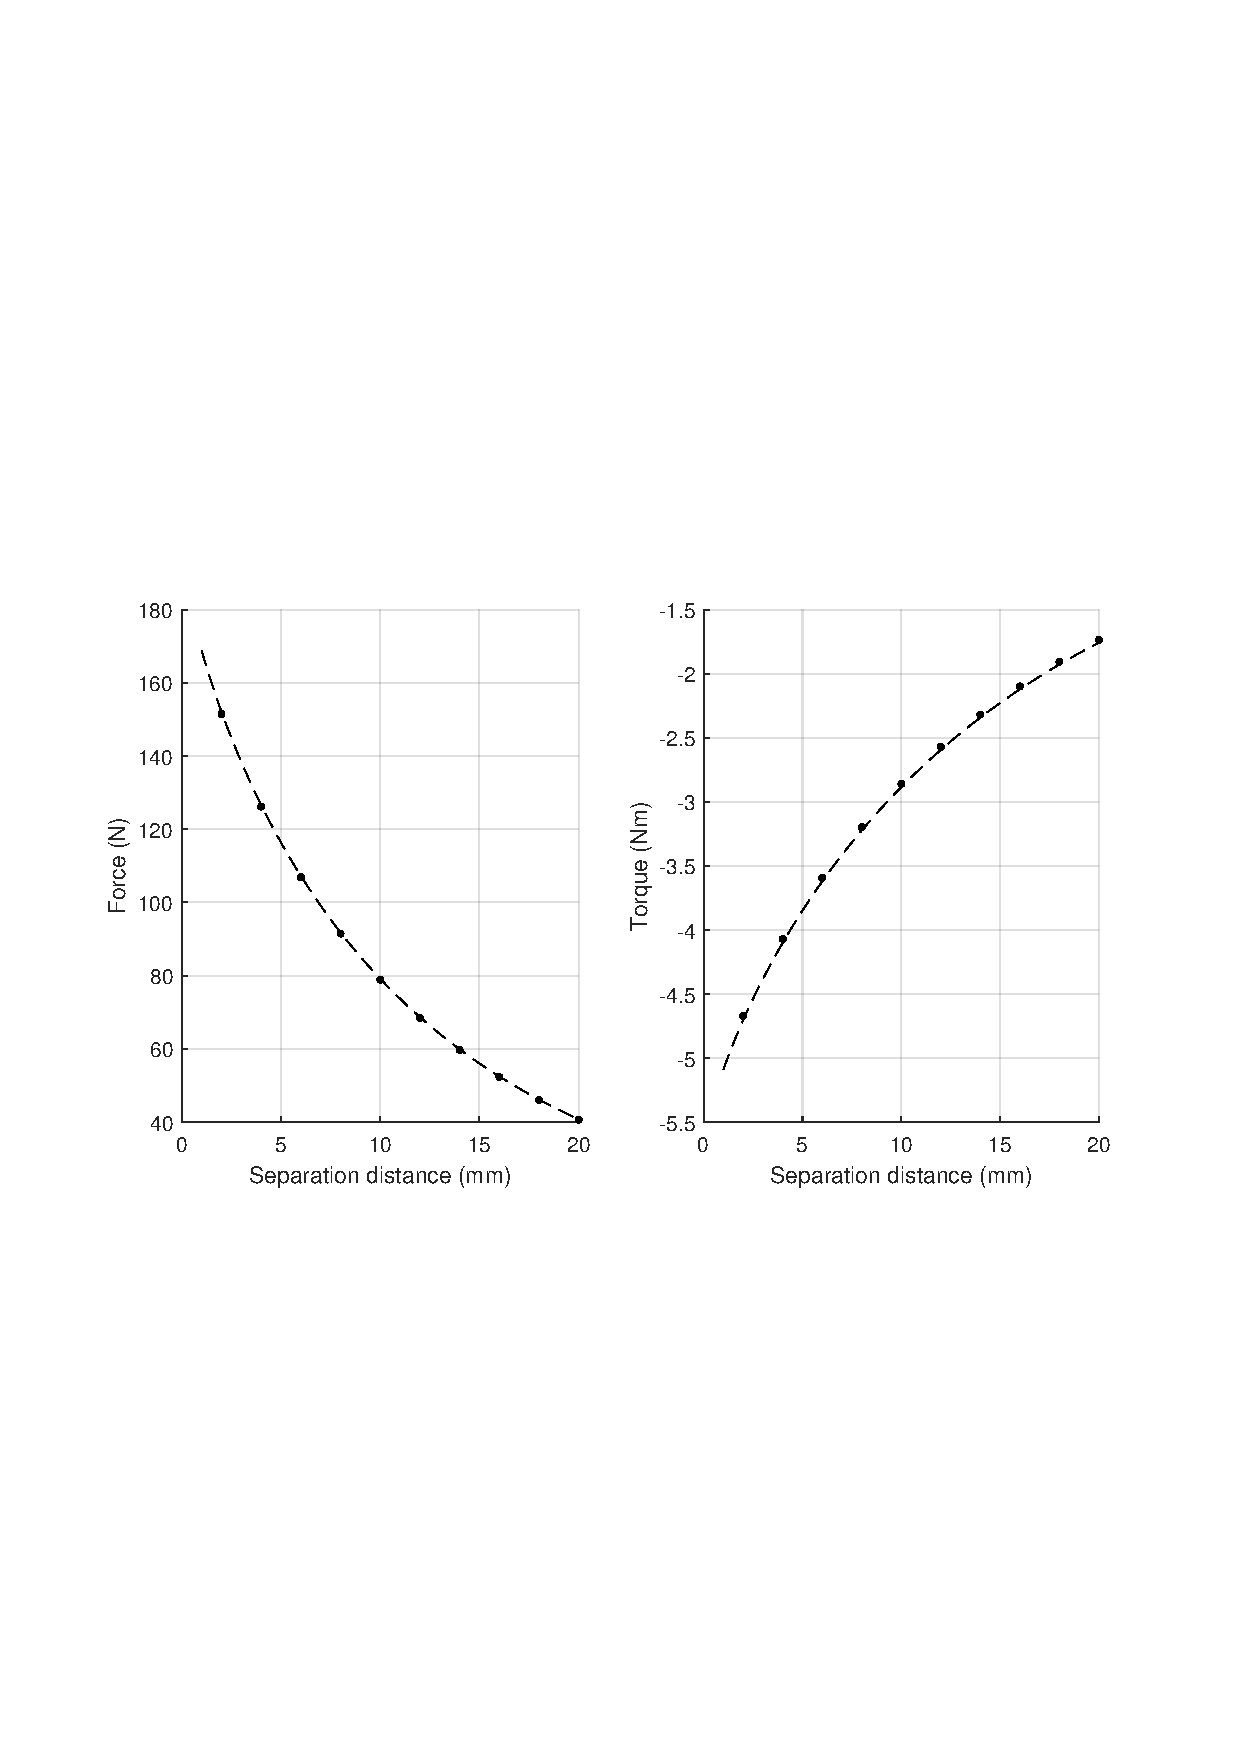
\includegraphics[trim = 3cm 9cm 3cm 9cm,width=0.9\linewidth]{p1/p1FIG6}
	\caption{The \(x\)-force and \(y\)-torque on magnet B shown in Figure \ref{fig:p1dodecahedra}. Both magnets are regular dodecahedra with edge lengths of 20mm. The torque is evaluated about the centre of magnet B. Dashed lines represent the force and torque evaluated using Algorithms \ref{alg:p1alg1} and \ref{alg:p1alg2}, and dots represent the results from finite element simulations. The results from both methods are in agreement, indicating correct results from Algorithms \ref{alg:p1alg1} and \ref{alg:p1alg2}.}
	\label{fig:p1dodecahedraresults}
\end{figure*}

The results obtained from Algorithms \ref{alg:p1alg1} and \ref{alg:p1alg2} align well with the finite element simulations. This indicates that the algorithms produce accurate force and torque results for non-cuboidal polyhedral magnets with non-parallel magnetisation vectors, further validating Algorithms \ref{alg:p1alg1} and \ref{alg:p1alg2}.

No analytic solutions for dodecahedral permanent magnets exist, so the error of Algorithms \ref{alg:p1alg1}, \ref{alg:p1alg2}, and the finite element simulations cannot be quantified. However, the solution time can still be analysed. Algorithms \ref{alg:p1alg1} and \ref{alg:p1alg2} were again considerably faster than the finite element simulations, with solutions being completed in approximately 4.96 seconds using 4608 triangular elements on the surface of magnet B, while each finite element simulation took approximately 40-50 seconds using an adaptive setup with a percent error of 1\% and approximately 18000 tetrahedral elements.
\section{Geometric optimisation}\label{sec:p1geometricOptimisation}
Algorithms \ref{alg:p1alg1} and \ref{alg:p1alg2} can be used for fast optimisation of magnetic systems. Presented here is one such case, wherein two pyramidal frustums are arranged with magnet B above magnet A, as shown in Figure \ref{fig:p1frustumcase}. Both magnets have a unit magnetisation strength of 1 Tesla. The magnetisation vectors are oppositely directed with the magnets in repulsion. The wall angle \(\theta\) is varied to maximise the force at a given distance while the magnet height and volume are kept constant at 5cm and 500cm\(^3\) respectively. A wall angle of \(\theta = 90^\circ\) corresponds to a cuboidal magnet with a height of 5cm and both width and depth of 10cm.
\begin{figure*}
	\centering
	\begin{subfigure}{0.4\textwidth}
		\centering
		\tdplotsetmaincoords{70}{110}
		\begin{tikzpicture}[scale=40,tdplot_main_coords]
		\coordinate(p1t) at (-0.050000,-0.050000,-0.000000);
		\coordinate(p2t) at (-0.050000,0.050000,-0.000000);
		\coordinate(p3t) at (0.050000,-0.050000,-0.000000);
		\coordinate(p4t) at (0.050000,0.050000,-0.000000);
		\coordinate(p5t) at (-0.025000,-0.025000,0.050000);
		\coordinate(p6t) at (0.025000,-0.025000,0.050000);
		\coordinate(p7t) at (-0.025000,0.025000,0.050000);
		\coordinate(p8t) at (0.025000,0.025000,0.050000);
		
		\coordinate(p1b) at (0.050000,0.050000,-0.025000);
		\coordinate(p2b) at (0.050000,-0.050000,-0.025000);
		\coordinate(p3b) at (-0.050000,0.050000,-0.025000);
		\coordinate(p4b) at (-0.050000,-0.050000,-0.025000);
		\coordinate(p5b) at (0.025000,0.025000,-0.075000);
		\coordinate(p6b) at (-0.025000,0.025000,-0.075000);
		\coordinate(p7b) at (0.025000,-0.025000,-0.075000);
		\coordinate(p8b) at (-0.025000,-0.025000,-0.075000);
		
		\draw[fill=white] (p4b) -- (p3b) -- (p1b) -- (p2b) -- cycle;
		\draw[fill=white] (p1b) -- (p3b) -- (p6b) -- (p5b) -- cycle;
		\draw[fill=white] (p1b) -- (p2b) -- (p7b) -- (p5b) -- cycle;
		
		\draw[fill=white] (p5t) -- (p6t) -- (p8t) -- (p7t) -- cycle;
		\draw[fill=white] (p2t) -- (p4t) -- (p8t) -- (p7t) -- cycle;
		\draw[fill=white] (p6t) -- (p8t) -- (p4t) -- (p3t) -- cycle;
		
		\node(A) at (-0.0375,-0.025,-0.08) {\text{A}};
		\node(B) at (-0.0375,-0.025,-0.005) {\text{B}};
		\end{tikzpicture}
		\caption{}
	\end{subfigure}
	~ \hspace{20pt}
	\begin{subfigure}{0.4\textwidth}
		\centering
		\tdplotsetmaincoords{90}{0}
		\begin{tikzpicture}[scale=40,tdplot_main_coords]
		\coordinate(p1t) at (-0.050000,-0.050000,-0.000000);
		\coordinate(p2t) at (-0.050000,0.050000,-0.000000);
		\coordinate(p3t) at (0.050000,-0.050000,-0.000000);
		\coordinate(p4t) at (0.050000,0.050000,-0.000000);
		\coordinate(p5t) at (-0.025000,-0.025000,0.050000);
		\coordinate(p6t) at (0.025000,-0.025000,0.050000);
		\coordinate(p7t) at (-0.025000,0.025000,0.050000);
		\coordinate(p8t) at (0.025000,0.025000,0.050000);
		
		\coordinate(p1b) at (0.050000,0.050000,-0.025000);
		\coordinate(p2b) at (0.050000,-0.050000,-0.025000);
		\coordinate(p3b) at (-0.050000,0.050000,-0.025000);
		\coordinate(p4b) at (-0.050000,-0.050000,-0.025000);
		\coordinate(p5b) at (0.025000,0.025000,-0.075000);
		\coordinate(p6b) at (-0.025000,0.025000,-0.075000);
		\coordinate(p7b) at (0.025000,-0.025000,-0.075000);
		\coordinate(p8b) at (-0.025000,-0.025000,-0.075000);
		
		\draw[gray] (p2b) -- (p4b) -- (p8b) -- (p7b) -- cycle;
		\draw[gray] (p1t) -- (p3t) -- (p6t) -- (p5t) -- cycle;
		
		\draw[<->] (0,0,-0.025) -- (0,0,0);
		\node (d) at (0.005,0,-0.0125) {\(d\)};
		
		\draw[->,thick] (0,0,0.035) -- (0,0,0.015);
		\node (M1) at (-0.0075,0,0.025) {\textbf{M}};
		\draw[->,thick] (0,0,-0.06) -- (0,0,-0.04);
		\node (M2) at (-0.0075,0,-0.05) {\textbf{M}};
		
		\node(theta1) at (-0.022,0,0.043){\(\theta\)};
		\node(theta2) at (-0.022,0,-0.068){\(\theta\)};
		\node(A) at (0.025,0,-0.05) {\text{A}};
		\node(B) at (0.025,0,0.025) {\text{B}};
		
		\end{tikzpicture}
		\caption{}
	\end{subfigure}
	\caption{Three-dimensional view (a) and side view (b) of two pyramidal frustum magnets with opposing vertical magnetisations \(\mathbf{M}\). Magnet B moves a distance \(d\) in the vertical direction. The wall angle \(\theta\) is varied while maintaining a constant magnet volume and height.}
	\label{fig:p1frustumcase}
\end{figure*}

The frustums were separated by a given distance \(d\) and the wall angle \(\theta\) varied. For all values of \(\theta\), the repulsive force between the magnets was calculated and divided by the maximum force for each separation to give the normalised force plot shown in Figure \ref{fig:p1frustumforce}. The peaks of this plot correspond to the maximum force at a given separation distance, and hence show the optimal wall angle for that distance. The optimal angle was calculated for several separation distances using this method with the results shown in Table \ref{tab:p1optimalfrustum}. It can be seen that the optimal wall angle increases with separation distance, indicating that as the magnets move further apart, the optimal shape tends toward a pyramid. On the contrary, as the magnets become closer, the optimal shape tends toward a cuboid.
\begin{figure}
	\centering
	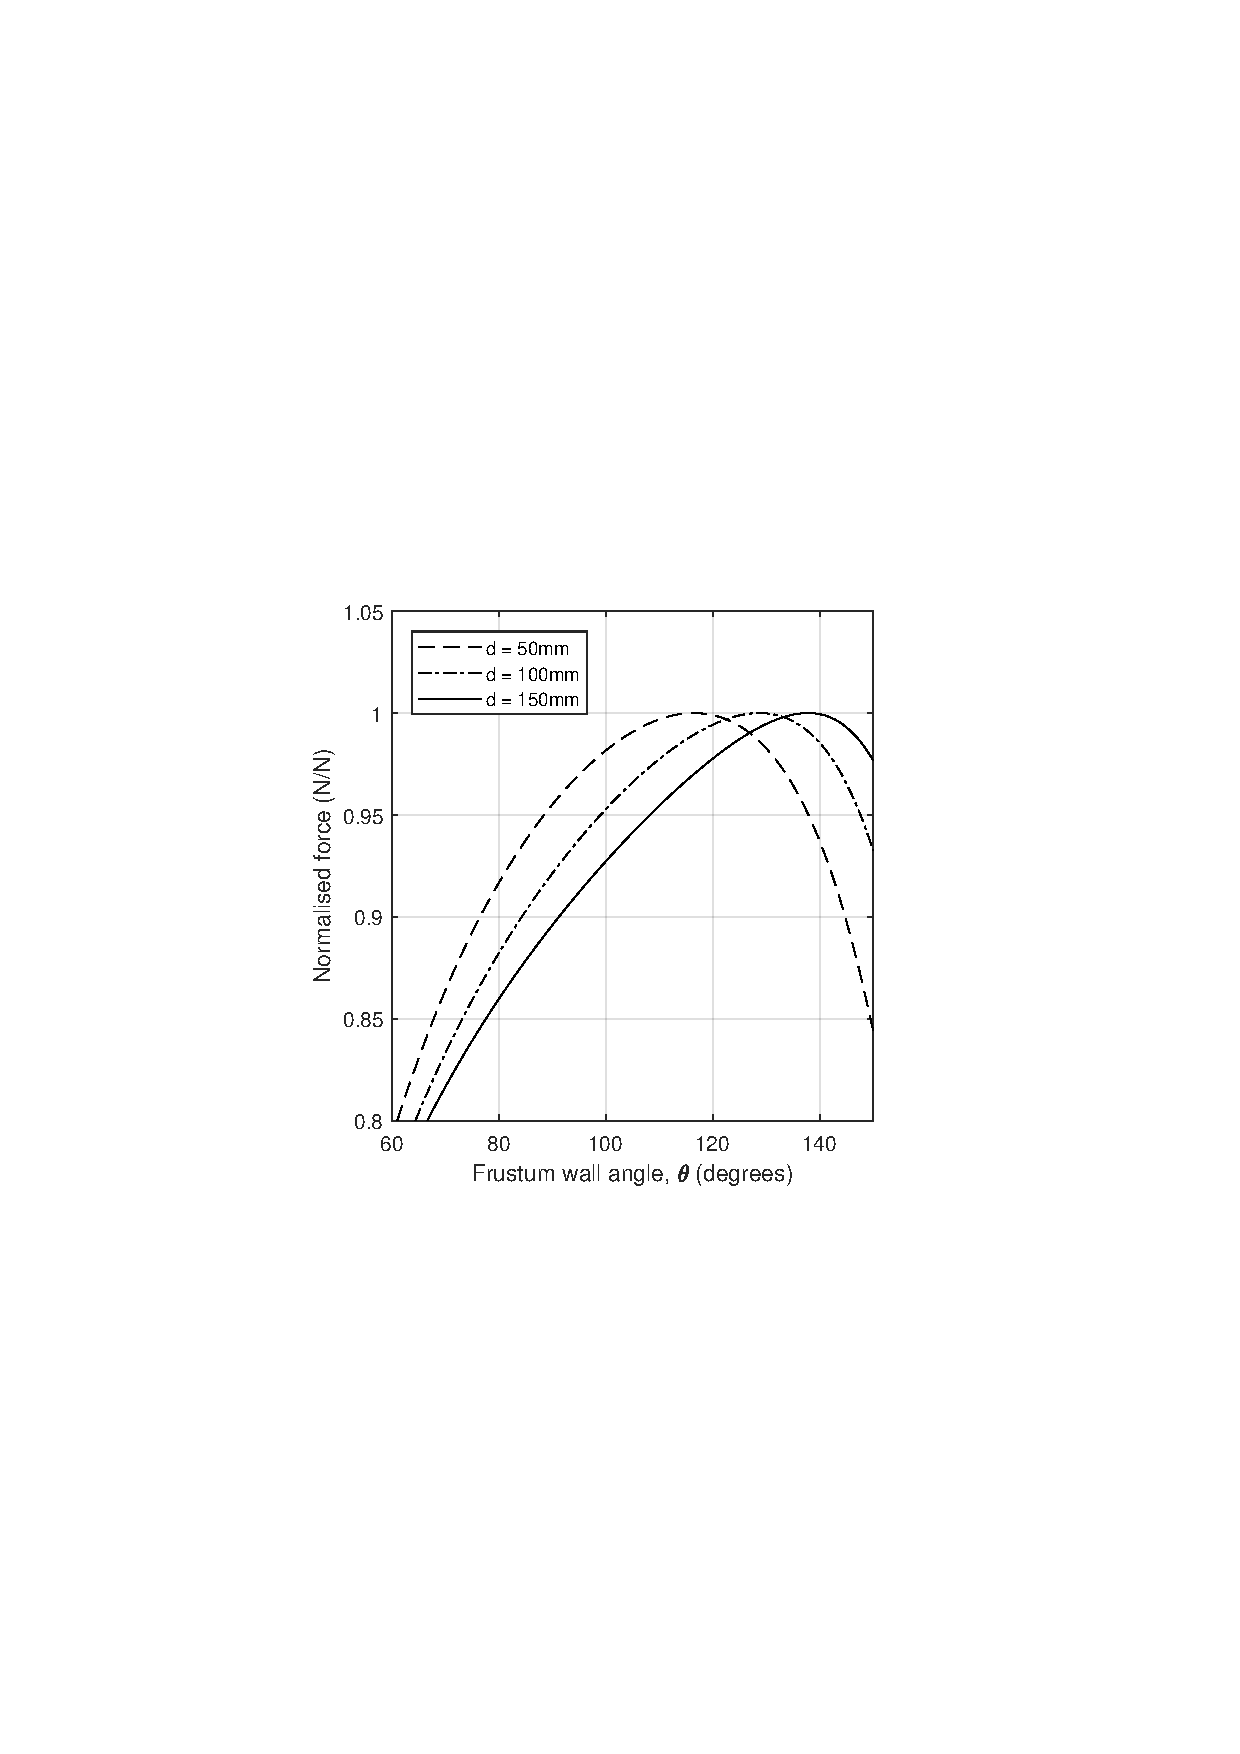
\includegraphics[trim = 5cm 9cm 5cm 9cm,width=0.8\linewidth]{p1/p1FIG8}
	\caption{The normalised force between the two frustum magnets shown in Figure \ref{fig:p1frustumcase} as the wall angle \(\theta\) is varied. Each plot corresponds to a given separation distance \(d\) shown in the legend. The normalised force is calculated by dividing the force at each point by the maximum force for each separation distance. The peak of each plot corresponds to the maximum force attained, and thus the optimal wall angle. As the separation distance increases, the peak moves to the right, indicating the optimum wall angle increases with the separation distance.}
	\label{fig:p1frustumforce}
\end{figure}
\begin{table}
	\centering
	\caption{The optimal wall angle of the pyramidal frustums at a given distance. This angle maximises the repulsive force between the magnets while maintaining a constant magnet volume and height.}
	\begin{tabular}{cc}
		\hline
		Separation distance (mm) & Optimal angle (degrees) \\
		\hline
		25 & 110 \\
		50 & 117 \\
		75 & 123 \\
		100 & 129 \\
		125 & 134 \\
		150 & 138 \\
		\hline
		\label{tab:p1optimalfrustum}
	\end{tabular}
\end{table}

The above test lead to an investigation on optimal angle for a varying separation distance. For a given separation distance, a golden ratio search was implemented to find the optimal angle which maximises the repulsive force. This was repeated for a large range of separation distances, and the plot shown in Figure \ref{fig:p1optimalfrustum} (left) was obtained. Again, it can be seen that the optimal angle increases with the separation distance. Interestingly, when the separation distance is zero, the optimal angle is not 90\(^\circ\). Namely, the optimal geometry is not cuboidal when the magnets are touching. Furthermore, the optimal angle is always greater than 90\(^\circ\), implying that cuboidal magnets are not the optimal geometry for this particular configuration.
\begin{figure*}
	\centering
	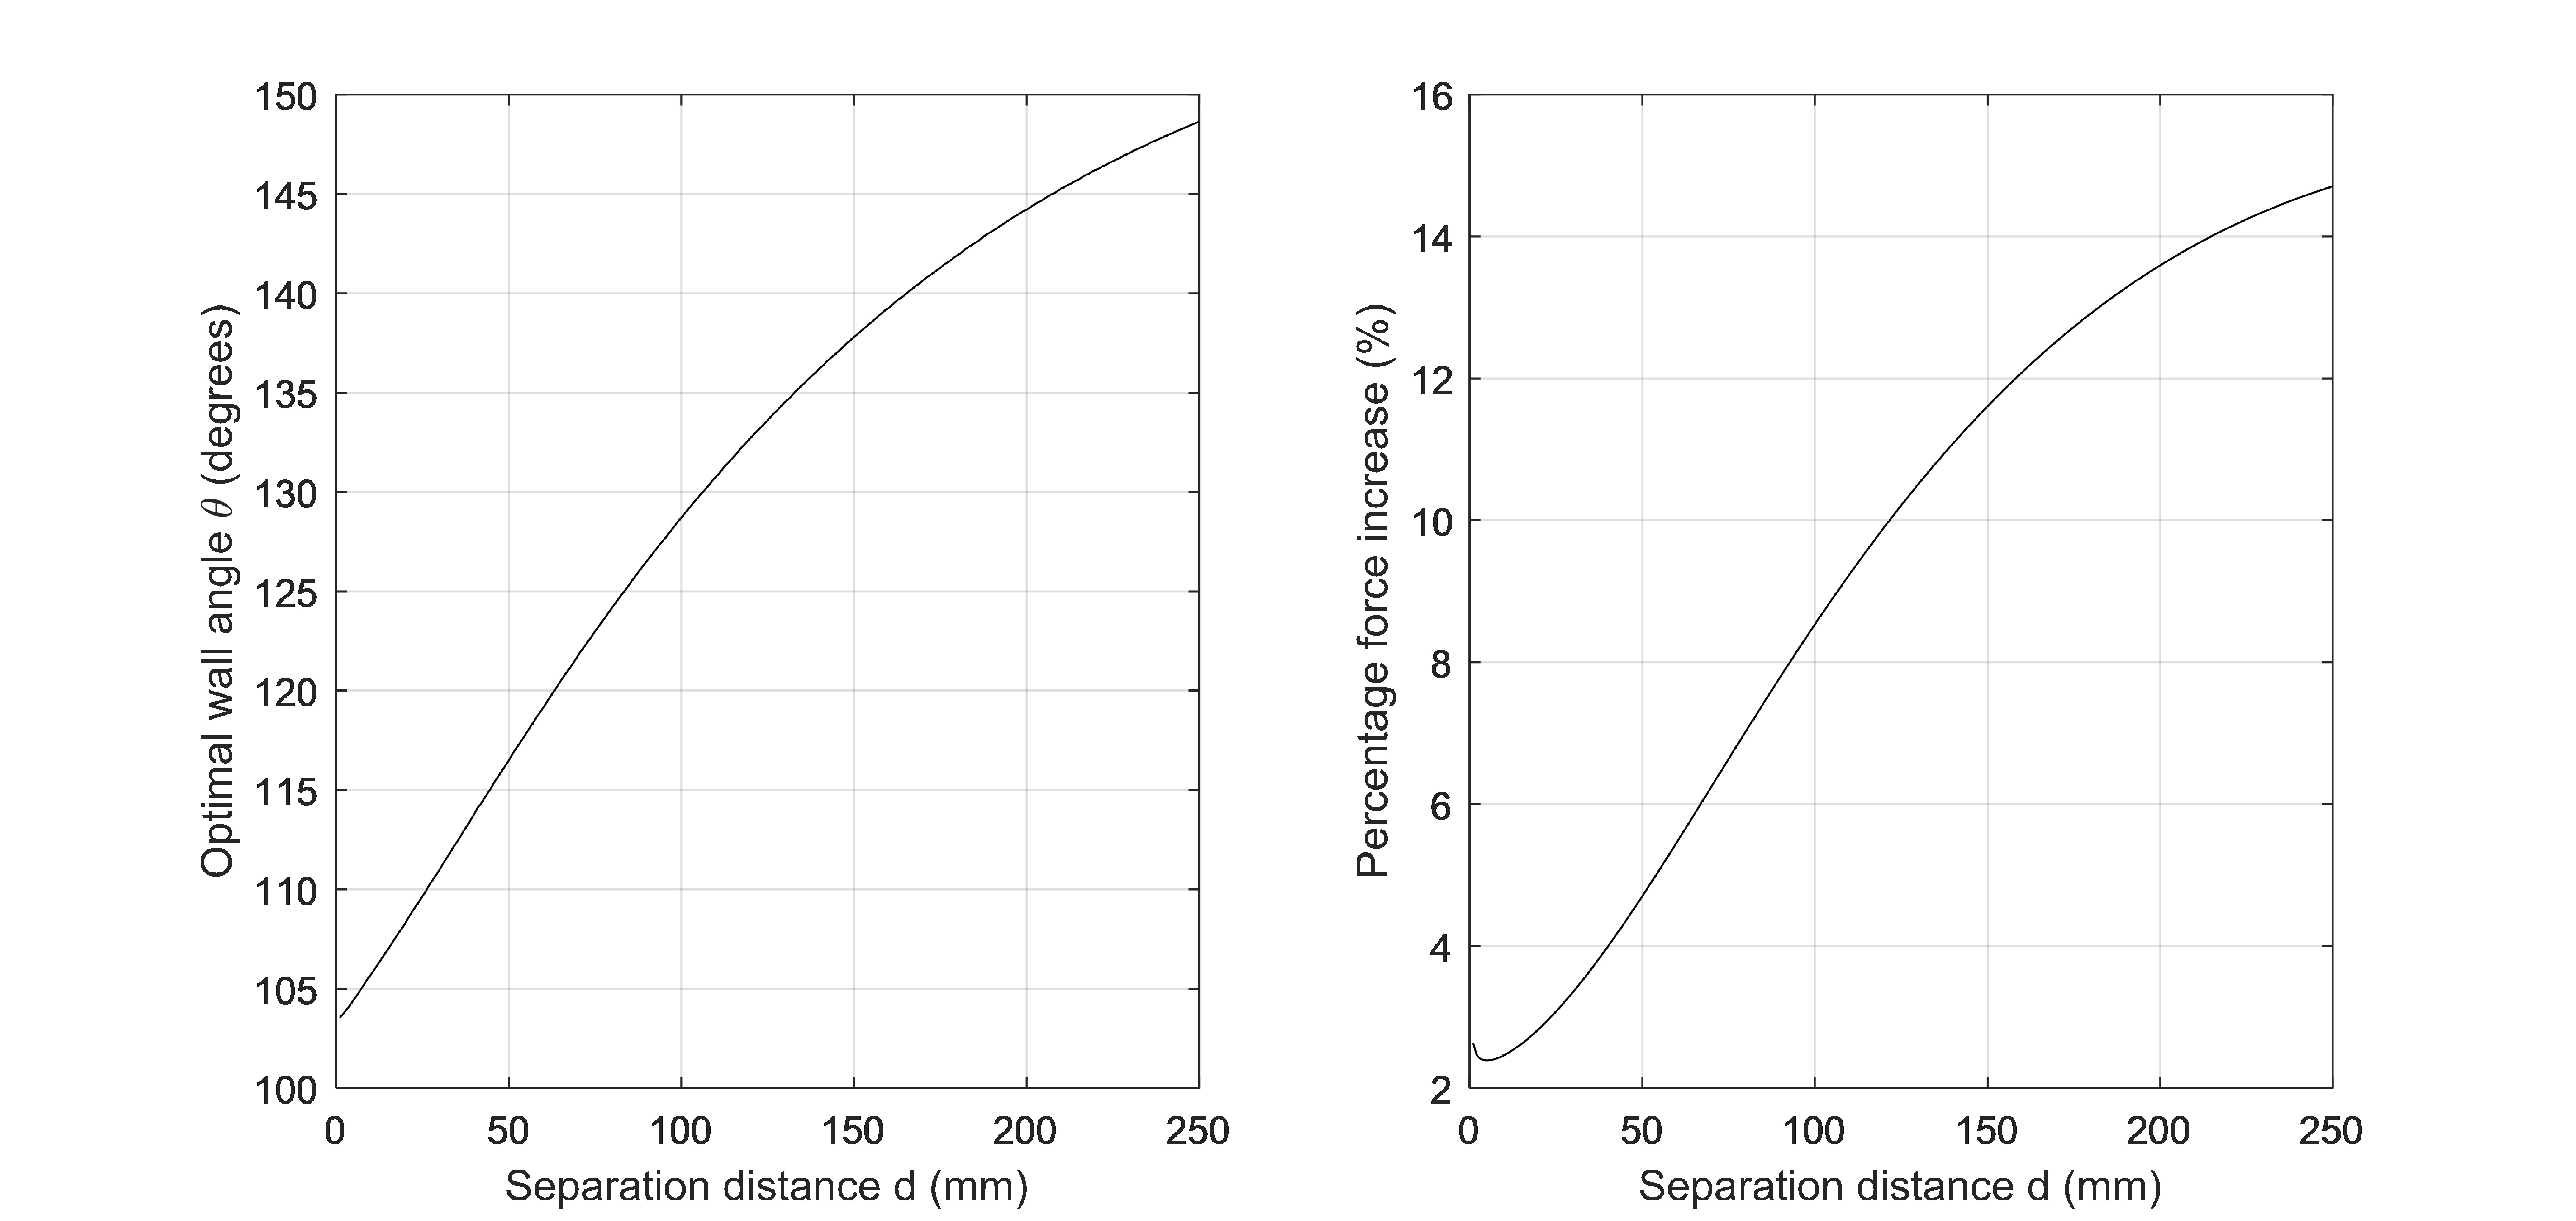
\includegraphics[trim = 4cm 0cm 4cm 0cm,width=\linewidth]{p1/p1FIG9}
	\caption{The optimal wall angle \(\theta\) of the frustums at a given distance to maximise the repulsive force between them (left). At all separation distances, the optimal angle is larger than 90\(^\circ\), indicating a cuboid is never the optimal geometry in this case. The optimal angle increases with separation distance, and tends toward a pyramid geometry at large separations. These results were compared to two cuboidal magnets with equal volume and height at the same separation distances. The force increase as a percentage of the repulsive force between the cuboids was found (right). A considerable increase in force was found, especially at larger separations. This implies that a larger force can be achieved with smaller mass if the system is optimised.}
	\label{fig:p1optimalfrustum}
\end{figure*}

In addition to calculating the optimal angle at a given separation distance, the percentage force increase was calculated. For each separation distance, the maximum force was found, as well as the force between two cuboidal magnets of equivalent height and volume. The percentage force increase is defined as
\begin{equation}
\text{PFI} = \frac{F_\text{frustum}-F_\text{cuboid}}{F_\text{cuboid}} \times 100\% \text{.}
\end{equation}
This percentage force increase was plotted against separation distance (Figure \ref{fig:p1optimalfrustum}, right). This value increases with separation distance, corresponding to a larger wall angle. Additionally, the force increase is positive for all separation distances, meaning with a constant magnetic volume, polyhedral magnets can achieve larger forces than cuboidal magnets. Alternatively, the same forces can be achieved using a smaller system mass, which could lead to significant cost savings.
\section{Conclusion}\label{sec:p1conclusion}
Permanent magnets are widely used in many industries and as such it is useful to characterise the interactions between them. This paper has outlined a fast semi-analytic method to calculate magnetic fields, forces, and torques of polyhedral permanent magnets. The development of two algorithms were discussed and implemented in Matlab. Several validation cases were considered, including a basic cuboid case and a more complicated system with dodecahedral magnets. These results were then validated against both literature (where possible) and finite element simulations. Then, a system with two pyramidal frustums was implemented in which the wall angle and separation distance could be varied while maintaining constant magnetic volume and height. The algorithms presented in this paper were used for rapid optimisation\footnote{Here, optimisation refers to maximising the force between two magnets of constant volume by varying magnet geometry. However, many forms of optimisation, such as optimisation of force per unit magnet height or torque per unit mass, may be used.} of this system, maximising the force between the magnets at a given distance. This resulted in the optimal angle being calculated over a large number of separations. Additionally, a considerable improvement in force over cuboidal magnets was found, showing standard magnetic geometries are not always optimal. The algorithms presented here can be used to further understand non-standard magnetic geometries, as well as optimise magnetic systems quickly to increase their performance.
\clearpage
\section*{Author's remarks on Chapter \ref{chap:paper1}}
The field equations presented in this chapter enable the evaluation of the magnetic field due to any polyhedral permanent magnet with constant uniform magnetisation and a relative permeability of unity. However, the methodology has several limitations that reduce the effectiveness of field evaluation. The most significant limitation is that of scaling; if the number of points at which the field is calculated is doubled, the methodology will take approximately twice as long to evaluate the field. This is because the entire process, including the deconstruction of the geometry, must be performed uniquely for each field point. In many situations, a large number of field points is desired, such as estimating forces and torques, optimising the field due to a magnet array (Chapter \ref{chap:paper3}), or modelling magnetic permeability (Chapter \ref{chap:paper4}). In addition, singularities in the equations exist for points on the same plane as the magnet facets. These limitations necessitate an alternative methodology which scales well with many field calculations and includes treatment of any singularities in the field equations.

\newpage
\section*{References}
\addcontentsline{toc}{section}{\protect\numberline{}References}
\printbibliography[heading=none]
\chapter{Magnetic field computation optimised for many points}\label{chap:paper2}
\fancyhead[LE]{\scshape Chapter\ \ref{chap:paper2}}
While Chapter \ref{chap:paper1} outlined a method to compute the magnetic field produced by an ideal polyhedral permanent magnet, several limitations existed in scaling with number of field points and singularity treatment. This chapter presents and validates a new field computation methodology which scales well with the number of field points and treats any singularities present in the field equations. Validation is performed using finite element analysis on magnetic systems with unity relative permeability. In contrast to the method outlined in Chapter \ref{chap:paper1}, the method detailed in this chapter only requires one deconstruction of geometry, independent of the number of field points. However, the field equations presented in this chapter are more complicated than those found in Chapter \ref{chap:paper1}. Therefore, when the field is computed at few points, the computational cost associated with more complicated field equations outweighs the advantage of only one deconstruction routine, and the method in Chapter \ref{chap:paper1} is preferred. In contrast, when the field is computed at many points, the method outlined in the current chapter greatly outperforms that from Chapter \ref{chap:paper1}.

Most applications, including those found in this thesis, are concerned with field calculations at many points, such as force and torque evaluations, optimisation of the field distribution (Chapter \ref{chap:paper3}), and permeability modelling (Chapter \ref{chap:paper4}). Thus, the method detailed in the current chapter is often the preferred method for magnetic field calculation due to a polyhedral permanent magnet.
%While the set of field equations presented in Chapter \ref{chap:paper1} are effective, they suffer from one main drawback, which limits the computation speed, especially when used for force and torque estimations. Although the field equations themselves are simple, the methodology requires processing of the geometry for each calculation. This processing is relatively expensive in computation time, and is required for every point the field is to be calculated at. Thus, if the field is to be evaluated at \(n\) points in space, the geometry processing algorithm must be performed \(n\) times, leading to longer calculation times. This is particularly problematic for force and torque estimations, where many field calculation must be performed for accurate estimations.
%To alleviate this, a new field calculation methodology was derived, and presented in this chapter. The field equations in this chapter are far more complicated than those seen in Chapter \ref{chap:paper1}, but the geometry processing is performed only once, regardless of the number of points the field is to be calculated at. Thus, if the field is to be evaluated at many points, the methodology in this chapter is far more effective, and is suggested for force and torque estimations.
%\newpage
\subsection*{Statement of authorship}
\renewcommand{\arraystretch}{1.5}
\begin{tabular}{m{0.25\textwidth} m{0.67\textwidth}}
    \hline \hline Paper title & Simplified equations for the magnetic field due to an arbitrarily-shaped polyhedral permanent magnet \\ \hline
    Publication status & Published \\ \hline
    Publication details & J. L. G. O’Connell, W. S. P. Robertson, and B. S. Cazzolato, ``Simplified equations for the magnetic field due to an arbitrarily-shaped polyhedral permanent magnet,'' Journal of Magnetism and Magnetic Materials, vol. 510, Sep. 2020, doi: 10.1016/j.jmmm.2020.166894. \\ \hline \hline
\end{tabular}

\vfill

\subsection*{Principal author}
\begin{tabular}{p{0.25\textwidth} m{0.67\textwidth}}
    \hline \hline Name & James O'Connell \\ \hline
    Contribution & \begin{itemize}
        \setlength\itemsep{-2mm}
        \item[-] Idea conceptualisation
        \item[-] Review of relevant literature
        \item[-] Developed polyhedral decomposition methodology
        \item[-] Performed all mathematical analysis, including computer-aided algebra and simplification of long and complication mathematical expressions
        \item[-] Identified singularities in the solutions for the field equations and treated these singularities, giving alternate formulations at the singular points
        \item[-] Implemented the algorithms in MATLAB code, including testing, analysis, and code optimisation
        \item[-] Created and executed finite element simulations to validate the mathematical algorithms and code implementation
        \item[-] Performed analysis of a polyhedral approximation of a cylindrical magnet
        \item[-] Wrote manuscript draft and created all figures
        \item[-] Finalisation of article
        \item[-] Preparation and submission for publication, including author correspondence
    \end{itemize} \\ \hline
    Percentage & 90\% \\ \hline
    Certification & This paper reports on original research conducted by the author during the period of Higher Degree by Research candidature and is not subject to any obligations or contractual agreements with a third party that would constrain its inclusion in this thesis. The author listed above is the primary author of this paper. \\ \hline
    Signature & \begin{tabular}{m{45mm} m{10mm} m{20mm}}
    \vspace{0.5mm}\includegraphics[width=0.3\textwidth]{jamesSignature.PNG} & Date: & 8 Dec 2021
    \end{tabular}
\end{tabular}

\vfill
    
\subsection*{Co-author contributions}
By signing this statement of authorship, each author certifies that:
\begin{enumerate}
    \item the candidate's stated contribution to the publication is accurate (as detailed above);
    \item permission is granted for the candidate to include the publication in the thesis; and
    \item the sum of all co-author contributions is equal to 100\% less the candidate's stated contribution.
\end{enumerate}
\begin{tabular}{m{0.25\textwidth} m{0.67\textwidth}}
    \hline \hline Name & Will Robertson \\ \hline
    Contribution & 5\% \\ \hline
    Signature & \vspace{2mm}\includegraphics[height=10mm]{willSig} \\  \hline
    Date & 16 Dec 2021 \\
    \hline \hline Name & Ben Cazzolato \\ \hline
    Contribution & 5\% \\ \hline
    Signature & \vspace{2mm} \includegraphics[height=10mm]{benSig} \\ \hline
    Date & 16 Dec 2021 \\
    \hline \hline \vfill
\end{tabular}
\renewcommand{\arraystretch}{1}
\newpage
%
\section*{\LARGE Simplified equations for the magnetic field due to an arbitrarily-shaped polyhedral permanent magnet}
James L.G. O'Connell, William S.P. Robertson, and Benjamin S. Cazzolato
\section*{Abstract}\addcontentsline{toc}{section}{\protect\numberline{}Abstract}\label{sec:p2abstract}
Due to their wide use in industrial and commercial devices, it is important to accurately and effectively model permanent magnets, leading to better magnet designs and more desirable magnetic characteristics. In recent decades, researchers have derived equations describing magnetic fields, forces, and torques, but these are usually limited to cuboid or ring-shaped magnets. Some authors have derived magnetic field equations for polyhedral magnets, allowing more general magnet shapes, but these are either not fully simplified or computationally inefficient. This paper presents a new set of simplified and exact equations describing the magnetic field produced by an arbitrarily-shaped polyhedral permanent magnet with constant uniform magnetisation and a relative permeability of unity. These equations were implemented in Matlab code and validated using finite element simulations and literature. These equations are significantly faster than finite element simulations, and can therefore be used for efficient optimisation of magnet geometry or topology, real-time simulations, and for approximation of curved surfaces of permanent magnets.
\section{Introduction}\label{sec:p2introduction}
Permanent magnets are used in a wide variety of applications, from microphones and loudspeakers to energy harvesting devices \cite{Coey2002}. They are an essential component of many electromechanical systems and are seeing widespread use with the current trend toward electric vehicles. In 2014, permanent magnets had an annual market of \$7bn USD, with hundreds of thousands of tons of neodymium magnets being manufactured annually \cite{Coey2014}. Permanent magnets see wide use in society, and it is therefore important to understand and model them effectively.

With the development of stronger magnetic materials in the late twentieth century, mathematical modelling of permanent magnets has become more common. Magnetic modelling has a high dependence on geometry, and as such, most research in this area has been undertaken on simple geometries such as cuboidal and ring-shaped permanent magnets.

Cuboid magnets are extremely prevalent in society and industry, and have therefore received considerable attention in literature. Additionally, their geometry is simple, leading to simple field equations. In 1984, \textcite{Akoun1984} published the magnetic field equations for a vertically-magnetised cuboid magnet by considering a magnetic charge distribution over the surface of the magnet. \textcite{Bancel1999} suggested that the magnetic field produced by a cuboid can be thought of as field contributions from each of the eight vertices, or `nodes'. Several decades later, \textcite{Ravaud2009} extended these equations to include an arbitrary magnetisation direction by using superposition of mutually perpendicular magnetisations. However, these equations do not consider mathematical singularities, which often exist at points inline with a magnet edge. Other authors have gone beyond field calculations by publishing equations describing forces and torques between parallel cuboid magnets with parallel magnetisations \cite{Akoun1984,Allag2009}, parallel cuboid magnets with arbitrary magnetisations \cite{Janssen2011}, and rotated cuboid magnets \cite{Dam2016}. However, all aforementioned equations are limited to cuboid magnets, and are invalid for other magnet geometries.

Like cuboid magnets, cylindrical and ring-shaped magnets have seen wide use in industry, and have also received considerable attention in literature. They exhibit simple geometry in a cylindrical coordinate system, leading to relatively simple field equations. In 1995, \textcite{Furlani1995} derived the magnetic field due to radially-magnetised ring sectors, but these equations are not fully analytic and require some numerical integration. Ravaud et al.\ \cite{Ravaud2008a,Ravaud2010} improved these equations by using elliptic integrals, leading to fewer numeric integrals. In another study, \textcite{Ravaud2008} considered the simpler geometry of a full ring magnet rather than a sector. With this assumption, they found expressions for the magnetic field produced by both radially- and axially-magnetised ring magnets using elliptic integrals. More recently, \textcite{Caciagli2018} derived simpler equations describing the magnetic field produced by cylindrical magnets. However, these equations are again limited to a specific geometry and other geometries require separate solutions.

Although cuboidal and ring magnets have been studied extensively, few other geometries have received attention. Papers by \textcite{Janssen2009,Janssen2010a}, \textcite{Compter2010}, \textcite{Rubeck2013}, and \textcite{OConnell2020} presented analytic equations for the magnetic field due to a general polyhedral permanent magnet with constant uniform magnetisation and unity relative permeability. These equations can be used for any magnet composed of flat faces, and can also be used to approximate curved surfaces, allowing approximate solutions of any magnet geometry. However, the studies by \textcite{Janssen2009,Janssen2010a} and \textcite{Compter2010} present equations which are not fully simplified, limiting their computational efficiency. The equations presented by \textcite{Rubeck2013} and \textcite{OConnell2020} are simpler, but inefficient for a large number of field evaluations because they require processing of the geometry for every field point. Furthermore, these studies do not consider mathematical singularities, which cause the magnetic field evaluations to become undefined at some locations.

This paper attempts to alleviate both of these issues by presenting new magnetic field equations for a general polyhedral permanent magnet which are fully simplified, computationally efficient, and include singularity treatment. These field equations are derived by the authors in Section \ref{sec:p2methodology} and validated using both past literature and finite element simulations in Section \ref{sec:p2validation} before the paper is concluded in Section \ref{sec:p2conclusion}.
\section{Methodology}\label{sec:p2methodology}
A permanent magnet with magnetisation vector \(\mathbf{M}\) can be modelled as a collection of magnetic charges described by the magnetic charge model \cite{Furlani2001}. The magnetic field \(\mathbf{B}\) at a point in space outside the magnet \(\mathbf{x}\) can be calculated using the charge model given by

\begin{equation}
\label{eqn:p2chargemodel}
\mathbf{B}\left( \mathbf{x} \right) = \frac{\mu_0}{4\pi} \left( \oint_{S} \left( \mathbf{M} \cdot \hat{\mathbf{n}} \right) \frac{\mathbf{x} - \mathbf{x}'}{\left| \mathbf{x} - \mathbf{x}' \right|^3} \ ds' - \int_{V} \left( \nabla \cdot \mathbf{M} \right) \frac{\mathbf{x} - \mathbf{x}'}{\left| \mathbf{x} - \mathbf{x}' \right|^3} \ dv' \right) \text{,}
\end{equation}

\noindent where \(\mu_0\) is the permeability of free space, \(V\) is the magnet volume, \(S\) is the magnet surface, \(\mathbf{x}'\) is a point in or on the magnet, and \(\hat{\mathbf{n}} = \left[ n_x, n_y, n_z \right]\) is the outward-facing unit normal vector of the magnet surface. If the magnet is assumed ideal; that is, the magnetisation \(\mathbf{M}\) is assumed uniform and constant and the relative permeability is assumed unity, the volume integral disappears as \(\nabla \cdot \mathbf{M} = 0\), leaving only the surface integral

\begin{equation}
\label{eqn:p2chargeB}
\mathbf{B}\left( \mathbf{x} \right) = \frac{\mu_0}{4\pi} \oint_{S} \left( \mathbf{M} \cdot \hat{\mathbf{n}} \right) \frac{\mathbf{x} - \mathbf{x}'}{\left| \mathbf{x} - \mathbf{x}' \right|^3} \ ds' \text{.}
\end{equation}

\noindent Equation (\ref{eqn:p2chargeB}) implies the magnet can be considered a set of \(n\) magnetically charged surfaces \(S_{\!i}\), with the total field given by

\begin{equation}
\label{eqn:p2chargeBdiscrete}
\mathbf{B}\left( \mathbf{x} \right) = \sum_{i=1}^n \frac{\mu_0}{4\pi} \int_{S_i} \left( \mathbf{M} \cdot \hat{\mathbf{n}}_i \right) \frac{\mathbf{x} - \mathbf{x}'}{\left| \mathbf{x} - \mathbf{x}' \right|^3} \ ds_i' = \sum_{i=1}^n \textbf{B}_i\left(\textbf{x}\right) \text{,}
\end{equation}

\noindent where \(\textbf{B}_i\left(\mathbf{x}\right)\) is the magnetic field contribution of the surface \(S_{\!i}\).

The total magnetic field due to the magnet can be found by solving Equation (\ref{eqn:p2chargeBdiscrete}), i.e., summing the field contributions from each surface \(S_{\!i}\) to give the total magnetic field. To do this, first the polyhedral magnet must be decomposed into a set of charged surfaces, as described in the following section.

\subsection{Polyhedral decomposition}\label{sec:p2polyhedrondecomposition}

To calculate the magnetic field at a point \(\mathbf{x} = \left[ x, y, z\right]\) due to a polyhedral permanent magnet with surface \(S\), the magnet is considered a collection of polygonal surfaces \(S_{\!i}\). The field calculation begins by considering one polygonal surface \(S_{\!i}\) with magnetic charge density \(\mathbf{M} \cdot \hat{\mathbf{n}}_i\), where \(\hat{\mathbf{n}}_i\) is the outward-facing unit normal vector of the surface \(S_{\!i}\). This surface and the point \(\mathbf{x}\) are rotated in 3D space about the origin such that \(S_{\!i}\) is parallel to the \(XY\)-plane; that is, \(S_{\!i}\) is rotated such that its normal vector is parallel to the \(z\)-axis. This is done by postmultiplying \(\mathbf{x}\) and each vertex of \(S_{\!i}\) by the rotation matrix \(R\), given by

\begin{equation}
R = \begin{bmatrix}
m & 0 & n_x \\[4pt]
-n_xn_y/m & n_z/m & n_y \\[4pt]
-n_xn_z/m & -n_y/m & n_z
\end{bmatrix} \text{,}
\end{equation}

\noindent where \(m = \sqrt{n_y^2+n_z^2}\). A full derivation of \(R\) is given in \ref{sec:p2Rderivation}. Note that if \(\hat{\mathbf{n}}_i = \left[\pm1,0,0\right]\), then the surface is parallel to the \(YZ\) plane and \(n_y = n_z = 0 \implies m = 0\) and \(R\) is undefined. In this case, the limit as \(n_z\) approaches 0 from the positive side is taken and \(R\) should instead be defined as

\begin{equation}
R = \begin{bmatrix}
\phantom{-}0 & 0 & 1 \\
\phantom{-}0 & 1 & 0 \\
-1 & 0 & 0 \end{bmatrix} \text{.}
\end{equation}

After rotation, the point at which the field is to be computed is given by \(\mathbf{x}_r = \mathbf{x}R\) and the surface \(S_{\!i}\) is parallel to the \(XY\)-plane. Lines are drawn through each vertex of the polygonal surface parallel to the \(y\)-axis, dividing the polygon into a series of trapezia \(T_{\!j}\), as shown in Figure \ref{fig:p2polyhedrondecomposition}. Note that for this work, a triangle is considered a degenerate case of a trapezium with one of the parallel sides having a length of zero. The magnetic field contribution of each trapezium is computed using the solution to Equation (\ref{eqn:p2chargeB}) described in Section \ref{sec:p2fieldcalc}.
\begin{figure}[h]
	\centering
	\begin{subfigure}{0.6\textwidth}
	\centering
	\begin{tikzpicture}[scale=2.5]
		\coordinate(c1) at (-0.47943,0.87758);
		\coordinate(c2) at (-0.98278,-0.18477);
		\coordinate(c3) at (-0.12797,-0.99178);
		\coordinate(c4) at (0.90369,-0.42818);
		\coordinate(c5) at (0.68648,0.72715);
	\draw (c1) -- (c2) -- (c3) -- (c4) -- (c5) -- cycle;
		\draw[->] (-1.2,-1.3) -- (-0.2,-1.3);
		\draw[->] (-1.2,-1.3) -- (-1.2,-0.3);		\node(x) at (-0.1,-1.3) {\(x\)};
		\node(y) at (-1.2,-0.2) {\(y\)};
		
		\node(Si) at (0,0) {\(S_i\)};
	\end{tikzpicture}
	\caption{}\label{fig:p2polyhedrondecompositiona}
\end{subfigure}

\vspace{40pt}

\begin{subfigure}{0.6\textwidth}
	\centering
	\begin{tikzpicture}[scale=2.5]
		\coordinate(c1) at (-0.98278,-0.18477);
		\coordinate(c2) at (-0.98278,-0.18477);
		\coordinate(c3) at (-0.47943,0.87758);
		\coordinate(c4) at (-0.47943,-0.65998);
		\filldraw[fill=red, fill opacity=0.1] (c1) -- (c2) -- (c3) -- (c4) -- cycle;
		\coordinate(c5) at (-0.47943,-0.65998);
		\coordinate(c6) at (-0.47943,0.87758);
		\coordinate(c7) at (-0.12797,0.83224);
		\coordinate(c8) at (-0.12797,-0.99178);
		\filldraw[fill=green, fill opacity=0.1] (c5) -- (c6) -- (c7) -- (c8) -- cycle;
		\coordinate(c9) at (-0.12797,-0.99178);
		\coordinate(c10) at (-0.12797,0.83224);
		\coordinate(c11) at (0.68648,0.72715);
		\coordinate(c12) at (0.68648,-0.54684);
		\filldraw[fill=cyan, fill opacity=0.1] (c9) -- (c10) -- (c11) -- (c12) -- cycle;
		\coordinate(c13) at (0.68648,-0.54684);
		\coordinate(c14) at (0.68648,0.72715);
		\coordinate(c15) at (0.90369,-0.42818);
		\coordinate(c16) at (0.90369,-0.42818);
		\filldraw[fill=magenta, fill opacity=0.1] (c13) -- (c14) -- (c15) -- (c16) -- cycle;
		\draw[->] (-1.2,-1.3) -- (-0.2,-1.3);
		\draw[->] (-1.2,-1.3) -- (-1.2,-0.3);		\node(x) at (-0.1,-1.3) {\(x\)};
		\node(y) at (-1.2,-0.2) {\(y\)};
		
		% Label trapezia
		\node(t1) at (-0.7,-0.2) {\(T_1\)};
		\node(t2) at (-0.3,-0.2) {\(T_2\)};
		\node(t3) at (0.3,-0.2) {\(T_3\)};
		\node(t4) at (0.77,-0.2) {\(T_4\)};
	\end{tikzpicture}
	\caption{}\label{fig:p2polyhedrondecompositionb}
\end{subfigure}

	\caption{After the polygonal surface \(S_{\!i}\) has been rotated such that it is parallel to the \(XY\)-plane (\subref{fig:p2polyhedrondecompositiona}), lines are drawn through each vertex parallel to the \(y\)-axis, dividing the polygon into trapezia (\subref{fig:p2polyhedrondecompositionb}).}
	\label{fig:p2polyhedrondecomposition}
\end{figure}

\subsection{Magnetic field calculation of charged trapezia}\label{sec:p2fieldcalc}

\begin{figure}
	\centering
	\def\lim{10}

\begin{tikzpicture}[scale=0.5]
	\coordinate(negx) at (-1,0);
	\coordinate(posx) at (\lim+2,0);
	\coordinate(negy) at (0,-5);
	\coordinate(posy) at (0,7);
	
	\coordinate(TL) at (1,6.5);
	\coordinate(BL) at (1,-3.5);
	\coordinate(TR) at (\lim,1);
	\coordinate(BR) at (\lim,-2);
	
	\draw[<->] (negx) -- (posx);
	\draw[<->] (negy) -- (posy);
	\filldraw[fill=black!5, fill opacity=0.8] (BL) -- (BR) -- (TR) -- (TL) -- cycle;
	
	\draw[dashed] (BL) -- (1,-5.5);
	\node(x1) at (1.25,-6) {\(x = x_1\)};
	\draw[dashed] (BR) -- (\lim,-5.5);
	\node(x2) at (\lim+0.25,-6) {\(x = x_2\)};
	\node(m1c1) at (6,-3.5) {\(y=m_1x+c_1\)};
	\node(m2c2) at (6,5.5) {\(y=m_2x+c_2\)};
	\node(x) at (\lim+2.5,0) {\(x\)};
	\node(y) at (0,7.4) {\(y\)};
\end{tikzpicture}
	\caption{A magnetically charged trapezial surface. It is parallel to the \(XY\)-plane with \(z\)-coordinate \(z = z'\) and a pair of opposite edges parallel to the \(y\)-axis.}
	\label{fig:p2trapezium}
\end{figure}

Given a magnetically charged trapezium parallel to the \(XY\)-plane at \(z = z'\), with the parallel lines having equations \(x = x_1\) and \(x = x_2\) and the non-parallel lines having equations \mbox{\(y = m_1x+c_1\)} and \mbox{\(y = m_2x+c_2\)} (shown in Figure \ref{fig:p2trapezium}), the magnetic field contribution \(\left[B_{xj},B_{yj},B_{zj}\right]\) at a point \(\mathbf{x}_r = \left[ x_r, y_r, z_r \right]\) is given by

\begin{equation}
	\label{eqn:p2myintegral}
	\left[ B_{xj}, B_{yj}, B_{zj} \right] = \frac{\mu_0}{4\pi} \int_{x_1}^{x_2} \int_{m_1x'+c_1}^{m_2x'+c_2} \left( \mathbf{M} \cdot \hat{\mathbf{n}} \right) \left[ I_x, I_y, I_z \right] \ dy' \ dx'
\end{equation}

\noindent where

\begin{align}
	I_x &= \frac{\left[x_r-x'\right]}{\left(\left(x_r-x'\right)^2+\left(y_r-y'\right)^2+\left(z_r-z'\right)^2\right)^{3/2}} \text{,} \nonumber \\
	I_y &=  \frac{\left[y_r-y'\right]}{\left(\left(x_r-x'\right)^2+\left(y_r-y'\right)^2+\left(z_r-z'\right)^2\right)^{3/2}} \text{,} \\
	I_z &=  \frac{\left[z_r-z'\right]}{\left(\left(x_r-x'\right)^2+\left(y_r-y'\right)^2+\left(z_r-z'\right)^2\right)^{3/2}} \text{.} \nonumber
\end{align}

After solving this difficult integral and simplifying the result\footnote{The full derivation for this solution is outlined in Appendix \ref{app:fieldEquations}}, the authors derived the following solution to Equation (\ref{eqn:p2myintegral}).

\begin{align}\label{eqn:p2fieldequation}
\begin{split}
B_{xj} &= \frac{\mu_0}{4\pi} \left(\mathbf{M} \cdot \hat{\mathbf{n}}\right) \sum_{p=1}^2 \sum_{q=1}^2 \left[ \left( -1 \right) ^{p+q} \left( \ln \left( T_{pq} \right) - \frac{m_p}{\sqrt{1+m_p^2}} \ln \left(S_{\!pq}\right) \right) \right] \\
B_{yj} &= \frac{\mu_0}{4\pi} \left(\mathbf{M} \cdot \hat{\mathbf{n}}\right) \sum_{p=1}^2 \sum_{q=1}^2 \left[ \left( -1 \right)^{p+q} \frac{1}{\sqrt{1+m_p^2}} \ln \left( S_{\!pq} \right) \right] \\
B_{zj} &= \frac{\mu_0}{4\pi} \left(\mathbf{M} \cdot \hat{\mathbf{n}}\right) \sum_{p=1}^2 \sum_{q=1}^2 \Bigg[ \left( -1 \right) ^{p+q} \arctan \left( U_{pq} \right) \Bigg] \text{,}
\end{split}
\end{align}

\noindent with

\begin{align}\label{eqn:p2intermediatevars}
\begin{split}
X &= x_q - x_r \\
Y &= c_p + m_px_q - y_r \\
Z &= z' - z_r \\
R_{pq} &= \sqrt{X^2 + Y^2 + Z^2} \\
S_{\!pq} &= X + m_pY + \sqrt{1+m_p^2}R_{pq} \\
T_{pq} &= R_{pq} + Y \\
U_{pq} &= \frac{m_p\left(X^2+Z^2\right)-XY}{ZR_{pq}} \text{.}
\end{split}
\end{align}

Equation (\ref{eqn:p2fieldequation}) describes the magnetic field produced by the magnetically charged trapezium shown in Figure \ref{fig:p2trapezium}. Further processing is required to calculate the magnetic field produced by a polyhedral magnet, as described in the following sections.

\subsubsection{Special case when \(m_p = 0\)}

Equation (\ref{eqn:p2fieldequation}) can be applied to a cuboidal magnet by using six rectangular faces with \(m_p = 0\) for all \(p\). Substituting \(m_p = 0\) into Equations (\ref{eqn:p2fieldequation}) and (\ref{eqn:p2intermediatevars}) gives the following simplified equations for a cuboidal magnet.

\begin{align}\label{eqn:p2cuboidequation}
\begin{split}
B_x &= \frac{\mu_0}{4\pi} \left(\mathbf{M} \cdot \hat{\mathbf{n}}\right) \sum_{p=1}^2 \sum_{q=1}^2 \left[ \left( -1 \right) ^{p+q} \ln \left( T_{pq} \right) \right] \\
B_y &= \frac{\mu_0}{4\pi} \left(\mathbf{M} \cdot \hat{\mathbf{n}}\right) \sum_{p=1}^2 \sum_{q=1}^2 \left[ \left( -1 \right) ^{p+q} \ln \left( S_{\!pq} \right) \right] \\
B_z &= \frac{\mu_0}{4\pi} \left(\mathbf{M} \cdot \hat{\mathbf{n}}\right) \sum_{p=1}^2 \sum_{q=1}^2 \left[ \left( -1 \right) ^{p+q} \arctan \left( U_{pq} \right) \right] \text{,}
\end{split}
\end{align}

\noindent with

\begin{align}\label{eqn:p2cuboidvars}
\begin{split}
X &= x_q - x_r \\
Y &= c_p - y_r \\
Z &= z' - z_r \\
R_{pq} &= \sqrt{X^2 + Y^2 + Z^2} \\
S_{\!pq} &= X + R_{pq} \\
T_{pq} &= R_{pq} + Y \\
U_{pq} &= \frac{-XY}{ZR_{pq}} \text{.}
\end{split}
\end{align}

It can be shown that these equations are equivalent to those published by \textcite{Akoun1984}, \textcite{Bancel1999}, and \textcite{Ravaud2009}, verifying Equation (\ref{eqn:p2fieldequation}) for cuboidal magnets\footnote{The equations in \cite{Akoun1984}, \cite{Bancel1999}, and \cite{Ravaud2009} are of the same form, but with different variable names.}.

\subsection{Polyhedral recomposition}

Once the magnetic field contributions from each trapezium \(T_{\!j}\) is computed, all contributions are summed to give the total field due to the polygonal surface \(S_{\!i}\),

\begin{equation}
\begin{bmatrix}
B_{xi} & B_{yi} & B_{zi}
\end{bmatrix} = \sum_j \begin{bmatrix}
B_{xj} & B_{yj} & B_{zj} \end{bmatrix} \text{.}
\end{equation}

\noindent This magnetic field vector is then postmultiplied by \(R^\text{T}\) to give the field due to \(S_{\!i}\) in the original coordinate system,

\begin{equation}
\textbf{B}_i\left(\textbf{x}\right) = \begin{bmatrix}
B_{xi} & B_{yi} & B_{zi} \end{bmatrix}
R^\textsf{T} \text{,}
\end{equation}

\noindent where \(R^{\textsf{T}}\) is the transpose of \(R\).

This process is repeated for each face of the polyhedron. Finally, the field contributions from each polygonal face \(S_{\!i}\) are summed to give the total magnetic field at the point \(\mathbf{x}\) due to the polyhedral permanent magnet,

\begin{equation}
\textbf{B}\left(\textbf{x}\right) = \sum_{i=1}^n \textbf{B}_i\left(\textbf{x}\right) \text{.}
\end{equation}

\subsection{Singularity treatment}

Singularities can be found in Equation (\ref{eqn:p2fieldequation}) when \(S_{\!pq} = 0\), when \(T_{pq} = 0\), or when \(U_{pq} = 0/0\). The regions in which each of these singularities occur are shown in Figure \ref{fig:p2singularities}. Under these conditions, the magnetic field given by Equation (\ref{eqn:p2fieldequation}) is undefined, so these singularities must be resolved to give a robust magnetic field solution.

\begin{figure}
	\centering
	\def\myscale{0.3}
\def\greythick{50}

\begin{subfigure}{0.45\textwidth}
\centering
\begin{tikzpicture}[scale=\myscale]
	\coordinate(TL) at (1,6.5);
	\coordinate(BL) at (1,-3.5);
	\coordinate(TR) at (10,1);
	\coordinate(BR) at (10,-2);
	
	% Draw some white lines to make sure all figures are the same size:
	\draw[white] (-4,8.5) -- (15,-1.5);
	\draw[white] (-4,-5.5) -- (15,0.5);
	\draw[white] (1,-7) -- (1,9);
	\draw[white] (11,-7) -- (11,9);
	
	% Draw the singular regions:
	\draw[gray!\greythick] (10,1) -- (15,-2.05555556);
	\draw[gray!\greythick] (10,-2) -- (15,-1.16666667);
	
	% Draw the trapezium:
	\filldraw[fill=black!5, fill opacity=0.8] (BL) -- (BR) -- (TR) -- (TL) -- cycle;
\end{tikzpicture}
\caption{}\label{fig:p2singularitiesa}
\end{subfigure}
\begin{subfigure}{0.45\textwidth}
\centering
\begin{tikzpicture}[scale=\myscale]
    \coordinate(TL) at (1,6.5);
    \coordinate(BL) at (1,-3.5);
    \coordinate(TR) at (10,1);
    \coordinate(BR) at (10,-2);
	
	% Draw some white lines to make sure all figures are the same size:
	\draw[white] (-4,8.5) -- (15,-1.5);
	\draw[white] (-4,-5.5) -- (15,0.5);
	\draw[white] (1,-7) -- (1,9);
	\draw[white] (11,-7) -- (11,9);
	
	% Draw the singular regions:
	\draw[gray!\greythick] (1,6.5) -- (1,9);
	\draw[gray!\greythick] (10,1) -- (10,9);
	
	% Draw the trapezium:
	\filldraw[fill=black!5, fill opacity=0.8] (BL) -- (BR) -- (TR) -- (TL) -- cycle;
\end{tikzpicture}
\caption{}\label{fig:p2singularitiesb}
\end{subfigure}
\begin{subfigure}{0.45\textwidth}
    \centering
    \begin{tikzpicture}[scale=\myscale]
    \coordinate(TL) at (1,6.5);
    \coordinate(BL) at (1,-3.5);
    \coordinate(TR) at (10,1);
    \coordinate(BR) at (10,-2);
	
	% Draw the singular regions:
	\draw[gray!\greythick] (-4,9.55555556) -- (15,-2.05555556);
	\draw[gray!\greythick] (-4,-4.33333333) -- (15,-1.16666667);
	\draw[gray!\greythick] (1,-7) -- (1,9);
	\draw[gray!\greythick] (10,-7) -- (10,9);
	
	% Draw the trapezium:
	\filldraw[fill=black!5, fill opacity=0.8] (BL) -- (BR) -- (TR) -- (TL) -- cycle;
\end{tikzpicture}
\caption{}\label{fig:p2singularitiesc}
\end{subfigure}


	\caption{The regions around a trapezium in which singularities occur. \(S_{\!pq} = 0\) along the grey lines in (\subref{fig:p2singularitiesa}), \(T_{pq} = 0\) along the grey lines in (\subref{fig:p2singularitiesb}), and \(U_{pq} = 0/0\) along the grey lines in (\subref{fig:p2singularitiesc}).}
	\label{fig:p2singularities}
\end{figure}

\subsubsection{Solving \(S_{\!pq} = 0\)}

Substituting \(S_{\!pq} = 0\) into Equation (\ref{eqn:p2intermediatevars}) implies that \(X < 0\), \(Y = m_pX\), and \(Z = 0\). Therefore, any point inline with one of the non-parallel edges and to the right of any trapezium, shown in Figure \ref{fig:p2singularitiesa}, will lead to a singularity in the equations. This can be solved by applying L'H\^{o}pital's rule twice, giving Equation (\ref{eqn:p2Ssingsol}).

When evaluating Equations (\ref{eqn:p2fieldequation}) and (\ref{eqn:p2intermediatevars}), if for any pair \(\left(p,q\right)\), \(X < 0\), \(Y = m_pX\), and \(Z = 0\), this singularity is solved by the redefinition

\begin{equation}\label{eqn:p2Ssingsol}
S_{\!pq} = \frac{1}{R_{pq}} \text{.}
\end{equation}

\subsubsection{Solving \(T_{pq} = 0\)}

Substituting \(T_{pq} = 0\) into Equation (\ref{eqn:p2intermediatevars}) implies that \(X = 0\), \(Y < 0\), and \(Z = 0\). Therefore, if a point is inline with one of the parallel edges of any trapezium and above it, shown in Figure \ref{fig:p2singularitiesb}, a singularity will occur. This can be solved by again applying L'H\^{o}pital's rule twice, giving Equation (\ref{eqn:p2Tsingsol}).

When evaluating Equations (\ref{eqn:p2fieldequation}) and (\ref{eqn:p2intermediatevars}), if for any pair \(\left(p,q\right)\), \(X = Z = 0\) and \(Y < 0\), this singularity is solved by the redefinition

\begin{equation}\label{eqn:p2Tsingsol}
T_{pq} = \frac{1}{R_{pq}} \text{.}
\end{equation}

\subsubsection{Solving \(U_{pq} = 0/0\)}

Setting the denominator of \(U_{pq}\) to 0 in Equation (\ref{eqn:p2intermediatevars}) gives \(Z = 0\) since \(R_{pq} > 0\) for any point not coincident with a vertex. If \(Z = 0\), then the numerator of \(U_{pq}\) also goes to 0 when either \(X = 0\) or \(Y = m_pX\). Therefore, this singularity occurs when \(Z = X = 0\), or when \(Z = Y - m_pX = 0\). The singular regions are shown in Figure \ref{fig:p2singularitiesc}.

Solving the former case, \(X = Z = 0\), requires the use of L'H\^{o}pital's rule once, giving \(U_{pq} = \sgn\left(Y\right)\). However, due to the summation over \(p\) and the term \(\left(-1\right)^{p+q}\) in Equation (\ref{eqn:p2fieldequation}), \(U_{pq}\) can simply be set to 0.

The latter case, namely, \(Z = Y - m_pX = 0\), has a more trivial solution. Since \(Y = m_pX\), the numerator simplifies to \(-m_pZ^2\), leaving \(U_{pq} = -m_pZ/R_{pq}\). Since \(Z = 0\) and \(R_{pq} > 0\), this becomes \(U_{pq} = 0\). These two results give Equation (\ref{eqn:p2Usingsol}).

When evaluating Equations (\ref{eqn:p2fieldequation}) and (\ref{eqn:p2intermediatevars}), if for any pair \(\left(p,q\right)\), \(Z = X = 0\) or \(Z = Y-mX = 0\), this singularity is solved by the redefinition

\begin{equation}\label{eqn:p2Usingsol}
U_{pq} = 0 \text{.}
\end{equation}

\subsection{Computational considerations}

In contrast with previous solutions \cite{Rubeck2013,OConnell2020}, the solution formulated in this paper has been derived to allow the computation of a matrix of points \(P\) to be evaluated with only a single polyhedral decomposition and rotation routine. If \(n\) points are defined as \(\left[x_1, y_1, z_1\right], \dotsc, \left[x_n, y_n, z_n\right]\), then \(P\) is defined by the \(\left( n \times 3\right)\) matrix

\begin{equation}
P = \begin{bmatrix}
x_1 & y_1 & z_1 \\
\vdots & \vdots & \vdots \\
x_n & y_n & z_n
\end{bmatrix} \text{.}
\end{equation}

For a given polygonal facet \(S_{\!i}\) with associated rotation matrix \(R\), \(P_r = PR\) gives a list of rotated points at which the magnetic field can be calculated. Equation (\ref{eqn:p2fieldequation}) is applied to each row of \(P_r\), and the magnetic field components rotated back to the original coordinate system after the computation of the field at all points in \(P_r\). In this way, polyhedron decomposition occurs only once, independent of the number of points, therefore reducing overhead and increasing efficiency.

Using this methodology on a polyhedron with \(E\) edges and \(F\) faces, a maximum of \(2E - F\) trapezia are required (see \ref{sec:p2numtrap}), giving an upper bound on the number of calculations required. If the magnetic field is to be evaluated at \(n\) points, then Equation (\ref{eqn:p2fieldequation}) must be computed a total of up to \(n\left(2E-F\right)\) times with up to \(2F\) total rotations. Therefore, if each computation of Equation (\ref{eqn:p2fieldequation}) takes \(t_n\) seconds and the average overhead for each calculation is \(t_o\), an upper bound for the total expected calculation time is

\begin{equation}
t_{\text{expected}} \leq \left(2E-F\right)\left(t_o + nt_n \right) \text{.}
\end{equation}

\noindent This equation shows that the calculation time scales approximately linearly with the number of points at which the field is calculated.

This methodology was implemented in vectorised Matlab code without parallelisation in Matlab R2017b (MathWorks, Inc., Natick, MA, USA). This was run on a workstation PC with an Intel Xeon E3-1240 v5 at 3.50GHz and 16GB of memory using Windows 10 Enterprise. In an effort to approximate the constants \(t_o\) and \(t_n\), a randomly generated polyhedron was defined, and the magnetic field calculated at a large number of points near the polyhedron. On this particular computer hardware, \(t_o\) was in the order of several milliseconds (\(10^{-3}\) seconds) and \(t_n\) was in the order of several hundred nanoseconds (\(10^{-7}\) seconds). These values will vary when using different computer hardware and software, but the constants stated here give an approximation of calculation time before the algorithm is executed.

This methodology excels when calculating the magnetic field at a large number of points. This is because the rotation and decomposition routines are the slowest parts of the algorithm, but only occur once, no matter the number of field calculations. The computation of Equation (\ref{eqn:p2fieldequation}) is orders of magnitude faster than the rotation and decomposition routine, and thus a larger number of field calculations has little effect on the computation time.

The Matlab implementation of the algorithm presented in this paper is available as the file polyhedronField.m at

\noindent \url{github.com/jlgO'Connell/polyhedralMagnet}.

\section{Validation}\label{sec:p2validation}
To validate this methodology, finite element simulations were performed using the Maxwell3D package from ANSYS Electronics Desktop 2018.0 (ANSYS, Inc., Berkeley, CA, USA). Two cases were considered, with the magnetic field of each being calculated analytically using the above methodology and numerically using Maxwell3D. The second case was further validated using the analytic solutions presented by \textcite{Caciagli2018}. The magnetic field for both cases was also calculated using methodology from previously published and validated work by the current authors \cite{OConnell2020}. In the subsequent sections, the results and computation time from the current methodology are compared to those of the finite element simulations, literature, and earlier work.

\subsection{Pyramid frustum magnet}

\begin{figure}
	\centering
	\def\lim{13}

\tdplotsetmaincoords{70}{45}
\begin{tikzpicture}[scale=0.13,tdplot_main_coords]

% Define coordinates:
\coordinate(ppb) at (15,15,-20);
\coordinate(pnb) at (15,-15,-20);
\coordinate(nnb) at (-15,-15,-20);
\coordinate(npb) at (-15,15,-20);
\coordinate(ppt) at (10,10,0);
\coordinate(pnt) at (10,-10,0);
\coordinate(nnt) at (-10,-10,0);
\coordinate(npt) at (-10,10,0);

% Fill in polygons:
\filldraw[fill=white] (ppt) -- (pnt) -- (nnt) -- (npt) -- cycle;
\filldraw[fill=white] (ppt) -- (ppb) -- (pnb) -- (pnt) -- cycle;
\filldraw[fill=white] (pnt) -- (nnt) -- (nnb) -- (pnb) -- cycle;

% Axes:
\draw[->] (0,0,0) -- (\lim,0,0);
\draw[->] (0,0,0) -- (0,\lim,0);
\draw[->] (0,0,0) -- (0,0,\lim);
\node(xaxis) at (\lim+2,0,0) {\(x\)};
\node(yaxis) at (0,\lim+2,0) {\(y\)};
\node(zaxis) at (0,0,\lim+2) {\(z\)};

% Dimensions:
\draw[<->] (20,-18,-20) -- (20,12,-20);
\node(botdim) at (26,-5,-20) {30mm};
\draw[<->] (-12,-20,-20) -- (18,-20,-20);
\node(botdim2) at (5,-26,-20) {30mm};
\draw[<->] (-15,-7,0) -- (-15,13,0);
\node(topdim) at (-21,6,0) {20mm};
\draw[<->] (-6,-15,0) -- (14,-15,0);
\node(topdim2) at (6,-21,0) {20mm};
\draw[<->] (17,17,-20) -- (17,17,0);
\node(height) at (21,21,-10) {20mm};

\end{tikzpicture}
	\caption{A square pyramid frustum permanent magnet. It has a base length of 30\si{\milli\metre}, a top length of 20\si{\milli\metre}, a height of 20\si{\milli\metre}, and a magnetisation of \num{1.035e6}\si{\ampere\per\metre} (1.3\si{\tesla}) in the positive \(z\) direction.}
	\label{fig:p2frustum}
\end{figure}

To validate Equation (\ref{eqn:p2fieldequation}) for non-cuboid magnets, the magnetic field due to the pyramid frustum permanent magnet shown in Figure \ref{fig:p2frustum} was computed. This frustum has a base length of 30\si{\milli\metre}, a top length of 20\si{\milli\metre}, a height of 20\si{\milli\metre}, and a magnetisation of \num{1.035e6}\si{\ampere\per\metre} (1.3\si{\tesla}) in the \(z\)-direction; i.e., a magnetisation vector of \(\left[0,0,1.035 \times 10^6\right]\)\si{\ampere\per\metre}. The magnetic field is measured across a plane positioned 1mm above the top surface of the frustum using a \(301\times301\) grid of points on a 30\si{\milli\metre} \(\times\) 30\si{\milli\metre} region (0.1\si{\milli\metre} grid spacing using 90601 gridpoints).

The geometry was input into both Maxwell3D and Matlab code, with the Maxwell3D simulation using approximately \num{1.2e6} tetrahedral elements (approx. \num{2e5} inside the magnet and \num{1e6} in the region outside the magnet). Both the Matlab code and Maxwell3D simulations were used to calculate the field across the previously mentioned \(301\times301\) grid of points above the frustum magnet, with results shown in Figure \ref{fig:p2frustumfield}.

The maximum field strength was 0.633\si{\tesla} (this work) and 0.636\si{\tesla} (FEA), giving a difference of 0.5 percent. Over the entire grid of points, the maximum error was 0.7 percent. This indicates that the analytic work presented in this paper is giving accurate field results. More detailed results are given in \ref{sec:p2detailedResults}.

The analytic work presented here and the FEA simulations calculate the magnetic field in very different ways, and as such it is difficult to compare the computation time for each method. For the frustum above, the FEA simulation took approximately 40 minutes, but the field can be found at any number of points after the simulation has been completed. In contrast, the analytic work presented here requires more computational time as the number of field points is increased. However, even with a relatively large number of field calculations, this algorithm took approximately 0.3 seconds to calculate the field at all 90601 points.

Finally, this calculation was validated using previous published and validated work by the current authors \cite{OConnell2020}. The error was within numerical noise, but the work presented in this paper was able to calculate the field orders of magnitude faster.

\begin{figure}
	\centering
	\begin{subfigure}{0.65\textwidth}
		\centering
		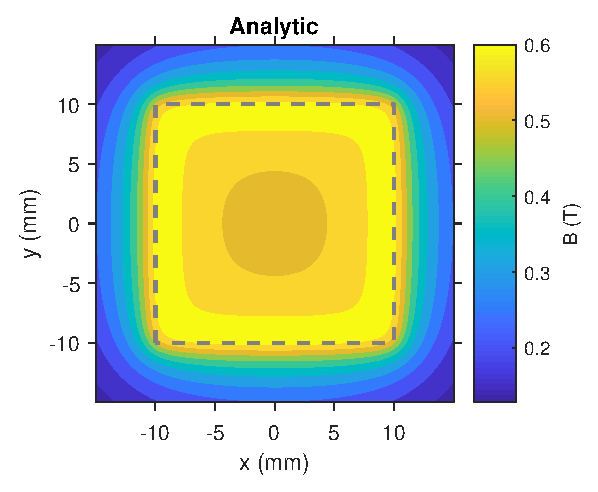
\includegraphics[width=\textwidth]{p2/p2FIG5a}
		\caption{}\label{fig:frustumfielda}\vspace{5mm}
	\end{subfigure}
	
	\begin{subfigure}{0.65\textwidth}
		\centering
		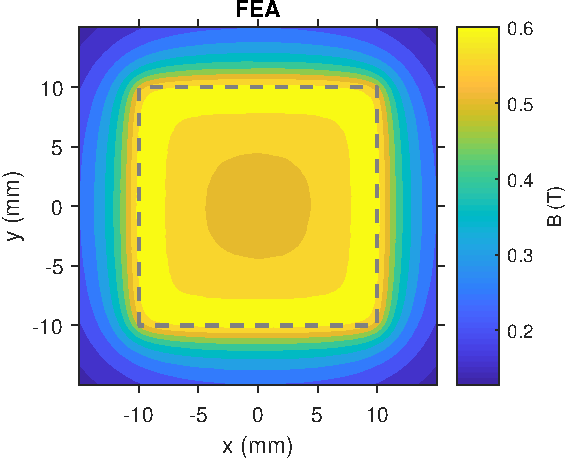
\includegraphics[width=\textwidth]{p2/p2FIG5b}
		\caption{}\label{fig:frustumfieldb}
	\end{subfigure}
	\caption{Magnetic field strength 1mm above the pyramid frustum magnet shown in Figure \ref{fig:p2frustum}, with the top surface of the magnet shown as a dashed line. The analytic calculation is shown in (\subref{fig:frustumfielda}), with the finite element calculation in (\subref{fig:frustumfieldb}). The maximum error between the two calculations is 0.7 percent, showing strong agreement.}
	\label{fig:p2frustumfield}
\end{figure}

\subsection{Cylindrical magnet}\label{sec:p2cylindricalmagnet}
\begin{figure}
	\centering
	\def\lim{13}

\tdplotsetmaincoords{70}{0}
\begin{tikzpicture}[scale=0.14,tdplot_main_coords]

% Draw cylinder
\draw (-10,0,-20) arc[radius = 10, start angle = -180, end angle = 0];
\draw (0,0,0) circle [radius = 10];
\draw (-10,0,0) -- (-10,0,-20);
\draw (10,0,0) -- (10,0,-20);

% Axes:
\draw[->] (0,0,0) -- (\lim,0,0);
\draw[->] (0,0,0) -- (0,0,\lim);
\node(xaxis) at (\lim+2,0,0) {\(x\)};
\node(zaxis) at (0,0,\lim+2) {\(z\)};

% Dimensions:
\draw[<->] (0,0,-27) -- (10,0,-27);
\node(radius) at (5,0,-30) {10mm};
\draw[<->] (-15,0,-20) -- (-15,0,0);
\node(height) at (-20,0,-10) {20mm};

\end{tikzpicture}
	\caption{A cylindrical permanent magnet. It has a radius of 10\si{\milli\metre}, a height of 20\si{\milli\metre}, and a magnetisation of \num{1.035e6}\si{\ampere\per\metre} (1.3\si{\tesla}) in the positive \(z\) direction.}
	\label{fig:p2cylinder}
\end{figure}
To further validate the analytic algorithm, a cylindrical geometry was examined, as shown in Figure \ref{fig:p2cylinder}. This magnet is an axially-magnetised cylindrical magnet with a radius of 10\si{\milli\metre}, a height of 20\si{\milli\metre}, and a magnetisation strength of \num{1.035e6}\si{\ampere\per\metre} (1.3\si{\tesla}). The magnetic field is again measured across a plane positioned \(z = 1\)\si{\milli\metre} above the top surface of the magnet using a \(301\times301\) grid of points on a 30\si{\milli\metre} \(\times\) 30\si{\milli\metre} region (0.1\si{\milli\metre} grid spacing using 90601 gridpoints).

Firstly, the exact magnetic field was calculated using the analytic equations published by \textcite{Caciagli2018}. Then, the geometry was input into Maxwell3D and a simulation carried out using approximately \num{9.6e5} tetrahedral elements (approximately \num{1.7e5} inside the magnet and \num{7.9e5} in the region outside the magnet). The cylinder was finally approximated as a polygonal prism, with the cross section being a 32-gon and an equivalent radius to maintain the same volume as the cylinder. Equation (\ref{eqn:p2fieldequation}) was applied to this polygonal prism to approximate the solution of a cylindrical magnet using a polyhedral magnet, and the results of all three calculations shown in Figure \ref{fig:p2cylinderfield}.

The maximum field strength was 0.571\si{\tesla} (this work), 0.573\si{\tesla} (FEA), and 0.571\si{\tesla} (exact \cite{Caciagli2018}). When compared to the exact result, the polyhedral approximation using this work gives a maximum error of less than 0.1 percent. When compared to the FEA simulation, the polyhedral approximation gave a maximum error of 0.8 percent. This implies the polyhedron is able to accurately approximate a cylindrical permanent magnet. More detailed results are given in \ref{sec:p2detailedResults}.

Again, it is difficult to compare the computation time of the algorithm presented in this paper and FEA simulations. The simulations took approximately 38 minutes to calculate the field at any number of points, whereas the algorithm here took approximately 0.9 seconds to calculate the field at 90601 points.

Additionally, this calculation was validated using previous published and validated work by the current authors \cite{OConnell2020}. The error was within numerical noise, but the algorithm presented in this paper calculated the field orders of magnitude faster.
\begin{figure}
	% Colour should be used for this figure
	\centering
	\begin{subfigure}{0.47\textwidth}
		\centering
		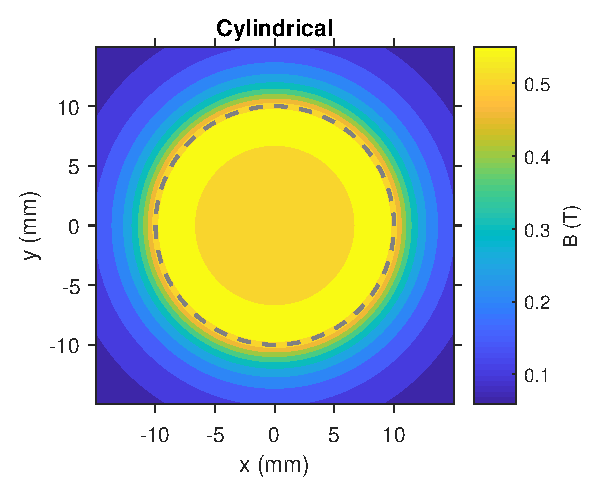
\includegraphics[width=\textwidth]{p2/p2FIG7a}
		\caption{}\label{fig:p2cylinderfielda}
	\end{subfigure}
	~
	\begin{subfigure}{0.47\textwidth}
		\centering
		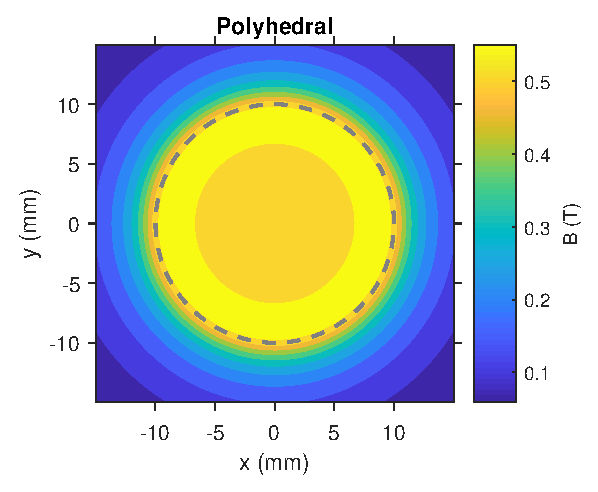
\includegraphics[width=\textwidth]{p2/p2FIG7b}
		\caption{}\label{fig:p2cylinderfieldb}
	\end{subfigure}
	
	\vfill
	\begin{subfigure}{0.47\textwidth}
		\centering
		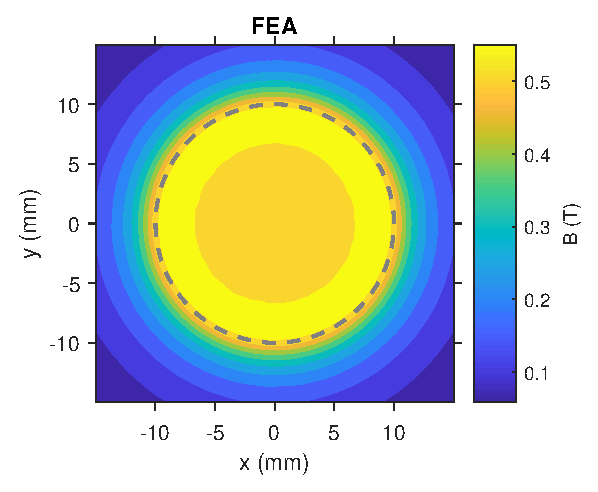
\includegraphics[width=\textwidth]{p2/p2FIG7c}
		\caption{}\label{fig:p2cylinderfieldc}
	\end{subfigure}
	\caption{Magnetic field strength 1\si{\milli\metre} above the cylindrical magnet shown in Figure \ref{fig:p2cylinder}, with the top surface of the magnet shown as a dashed line. The analytic cylindrical field \cite{Caciagli2018} is shown in (\subref{fig:p2cylinderfielda}), the polyhedral field shown in (\subref{fig:p2cylinderfieldb}), and the finite element calculation in (\subref{fig:p2cylinderfieldc}). The maximum percentage error between the exact cylinder field \cite{Caciagli2018} and polyhedral field was less than 0.1 percent, indicating it is an accurate approximation to a cylindrical magnet.}
	\label{fig:p2cylinderfield}
\end{figure}

\subsection{Polyhedral approximation of curved surfaces}
In the previous section, it was shown that an extruded 32-gon magnet is able to accurately approximate an axially-magnetised cylindrical magnet. This was validated using slow FEA simulations and the much faster analytic solution published by \textcite{Caciagli2018}. However, no analytic field solutions for general curved surfaces exist in literature, and FEA is slow and is impractical for real-time simulations. Instead, polyhedra can be used to approximate these surfaces for a fast-solving and accurate solution. To produce more accurate results, a polyhedron with a larger number of faces can be used; to achieve a faster calculation, a polyhedron with fewer faces can be used. This section shows an example of this tradeoff between accuracy and calculation time by approximating a cylindrical magnet with an extruded polygon with a varying number of sides, \(n\).

To quantify the error of the polyhedral approximation, the cylindrical magnet defined in Section \ref{sec:p2cylindricalmagnet} was considered. The magnetic field produced by this magnet was calculated using the equations published by \textcite{Caciagli2018} at a point 1\si{\milli\metre} above the central axis of the magnet, \(\mathbf{x} = \left[ 0, 0, 1\right]\)\si{\milli\metre}, and a point 1\si{\milli\metre} above the circumference of the top surface, \(\mathbf{x} = \left[ 10, 0, 1 \right]\)\si{\milli\metre}. The magnet was then approximated as a regular polygonal prism with a given number of sides \(n\), and the magnetic field calculated at the two aforementioned points. As the number of sides of the polygon \(n\) was increased, the error between the fields produced by cylindrical magnet and polyhedral magnet was calculated and recorded.

At the point \(\mathbf{x} = \left[ 0,0,1\right]\)\si{\milli\metre}, the exact magnetic field strength \cite{Caciagli2018} is 0.52\si{\tesla}. For a point along the axis of this magnet, the field can also be found using the difference between two cosines, giving the same result. The percentage error between this value and the magnetic field strength due to a polyhedral approximation was calculated for each \(n\) and is shown in Figure \ref{fig:p2polycylapproxa}. The polyhedral approximation is most impactful near the curved surface of the magnet, since this is where the geometry has been changed most significantly. Therefore, at the point \(\mathbf{x} = \left[ 0,0,1\right]\)\si{\milli\metre}, the polyhedral approximation is negligible and the error small since this point is far from the curved surface. The \(n = 32\) approximation from Section \ref{sec:p2cylindricalmagnet} takes approximately 28\si{\milli\second} to calculate the field and gives an error of \num{2.4e-5} percent. Alternatively, halving the number of sides (\(n = 16\)) takes approximately 17\si{\milli\second} to calculate the field while giving a larger error of \num{4.1e-4} percent.

At the point \(\mathbf{x} = \left[ 10,0,1\right]\)\si{\milli\metre}, the exact magnetic field strength \cite{Caciagli2018} is 0.53\si{\tesla}. The error between this field strength and the field strength due to the polyhedral approximation was again calculated and is shown in Figure \ref{fig:p2polycylapproxb}. This point is significantly closer to the curved surface of the magnet, and the error is therefore larger than at the point \(\left[ 0,0,1\right]\)\si{\milli\metre}. However, the error is still negligible for sufficiently large \(n\). The \(n = 32\) approximation from Section \ref{sec:p2cylindricalmagnet} takes approximately 29\si{\milli\second} to calculate the field and gives an error of \num{2.8e-2} percent. Alternatively, halving the number of sides (\(n = 16\)) takes approximately 16\si{\milli\second} to calculate the field while giving a larger error of \num{4.5e-1} percent.
\begin{figure}
	\centering
	\begin{subfigure}{0.6\textwidth}
		\centering
		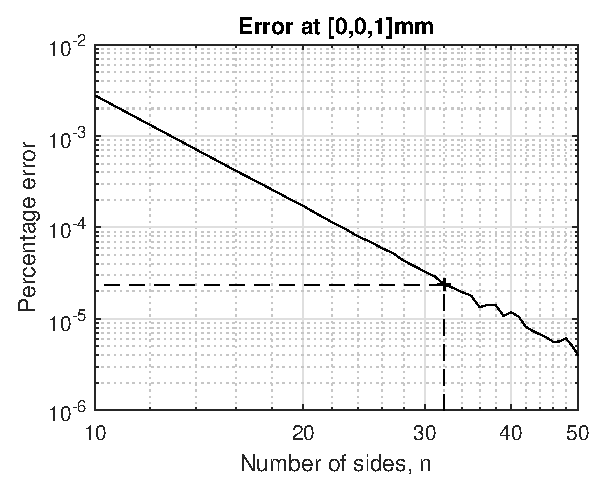
\includegraphics[width=\textwidth]{p2/p2FIG8a}
		\caption{}\label{fig:p2polycylapproxa}
	\end{subfigure}
	
	\begin{subfigure}{0.6\textwidth}
		\centering
		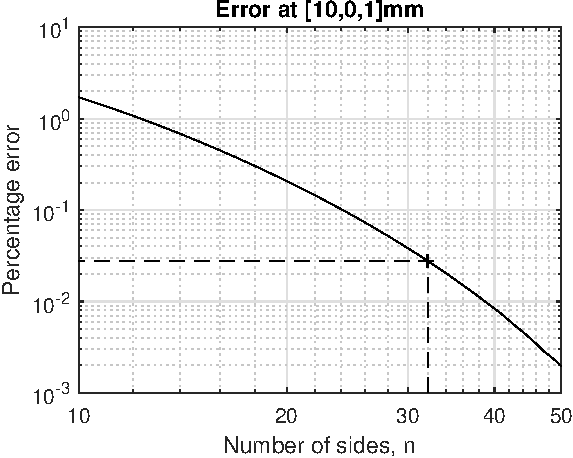
\includegraphics[width=\textwidth]{p2/p2FIG8b}
		\caption{}\label{fig:p2polycylapproxb}
	\end{subfigure}
	\caption{Error in the magnetic field strength produced by a polygonal prismatic magnet approximation of a cylindrical magnet as the number of sides of the polygon, \(n\), is increased. The \(n = 32\) approximation from Section \ref{sec:p2cylindricalmagnet} is highlighted. At the point \(\mathbf{x} = \left[0,0,1\right]\)\si{\milli\metre} (\subref{fig:p2polycylapproxa}), the magnetic field strength is 0.52\si{\tesla}, leading to an error of \num{2.4e-5} percent for a 32-gon approximation. At the point \(\mathbf{x} = \left[10,0,1\right]\)\si{\milli\metre} (\subref{fig:p2polycylapproxb}), the magnetic field strength is 0.53\si{\tesla}, leading to an error of \num{2.8e-2} percent for a 32-gon approximation.}
	\label{fig:p2polycylapprox}
\end{figure}

These results indicate that polyhedral permanent magnets can be used to approximate curved magnets and that a larger number of polygonal surfaces leads to a more accurate solution at the cost of a larger calculation time. Additionally, as the point \(\mathbf{x}\) approaches a curved magnet surface, a greater number of polyhedral facets are required for accurate field computations. This is particularly useful for magnet geometries with no analytic solution such as general curved surfaces. This approximation is considerably faster than FEA simulations, while maintaining high accuracy.
\section{Conclusion}\label{sec:p2conclusion}
This paper has outlined a new fully analytic and fast method for calculating the magnetic field produced by a polyhedral permanent magnet. The methodology was presented, outlining the process of decomposition and giving the solution to the charge model for a charged trapezium, leading to the total field produced by the polyhedral magnet. Singular regions were identified, and their solutions presented. This was followed by a validation section showing strong agreement between finite element simulations, literature, and the work detailed here. The magnetic field equations presented here are less complicated and more efficient than those in current literature since only two rotations are required per facet, independent of the number of magnetic field calculations.

The equations had high accuracy when compared to finite element simulations and literature using both a pyramid frustum magnet and a cylindrical magnet. The equations were validated against the finite element simulations and literature, giving a maximum error of less than 1 percent for both the frustum and cylindrical magnets.

It was shown that curved surfaces can be approximated as polyhedral surfaces and this methodology applied. A cylindrical magnet was approximated as a polygonal prism with an arbitrary number of sides. It was shown that both the accuracy and computation time increased with the number of sides. For the case considered, it was shown that the error was less than 0.1 percent using a 32-gon prismatic magnet, taking less than 30\si{\milli\second} to compute the field.

Currently, finite element simulations are usually used to analyse complicated magnetic systems. However, this is slow and optimisation of magnet shape or topology can take a considerable amount of time. The methodology presented here can be used to analyse these complicated magnetic systems far more quickly than finite element simulations. Furthermore, due to the simplicity and speed of calculation, it can be used for approximation of complicated magnet shapes, real-time simulations, or optimisation of magnet shape and topology to quickly arrive at a desired magnetic field.
\begin{subappendices}
\addcontentsline{toc}{section}{\protect\numberline{}Appendices}
\addtocontents{toc}{\protect\setcounter{tocdepth}{-1}}
\renewcommand{\thesection}{Appendix \arabic{chapter}.\Alph{section}}
\section{Derivation of \texorpdfstring{\(R\)}{R}}\label{sec:p2Rderivation}
The derivation of the rotation matrix \(R\) begins by defining a coordinate system on an arbitrary plane containing the polygonal surface \(S_{\!i}\). Let \(\left[ \hat{\mathbf{x}}, \hat{\mathbf{y}}, \hat{\mathbf{z}}\right]\) be the global coordinate system and let \(\hat{\mathbf{n}} = \left[ n_x, n_y, n_z\right]\) be the outward-facing unit normal vector of \(S_{\!i}\). We want to rotate this normal vector using the rotation matrix \(R\) such that \(\hat{\mathbf{n}} R = \hat{\mathbf{z}}\).

To do this, a coordinate system \(\left[ \hat{\mathbf{x}}', \hat{\mathbf{y}}', \hat{\mathbf{z}}' \right]\) is defined on the arbitrary plane such that \( \hat{\mathbf{n}} = \hat{\mathbf{z}}'\). To rotate \(\left[ \hat{\mathbf{x}}', \hat{\mathbf{y}}', \hat{\mathbf{z}}' \right]\) to \(\left[ \hat{\mathbf{x}}, \hat{\mathbf{y}}, \hat{\mathbf{z}}\right]\), a rotation matrix given by

\begin{equation}
R = \begin{bmatrix}
\hat{\mathbf{x}}'^{\textsf{T}} & \hat{\mathbf{y}}'^{\textsf{T}} & \hat{\mathbf{z}}'^{\textsf{T}}
\end{bmatrix}
\end{equation}

\noindent can be used.

Now, we have already defined

\begin{equation}
\hat{\mathbf{z}}' = \hat{\mathbf{n}} = \left[ n_x, n_y, n_z \right] \text{,}
\end{equation}

\noindent and \(\hat{\mathbf{x}}'\) and \(\hat{\mathbf{y}}'\) can be defined arbitrarily, provided \(\hat{\mathbf{x}}'\), \(\hat{\mathbf{y}}'\), and \(\hat{\mathbf{z}}'\) are mutually orthogonal unit vectors.

Without loss of generality, define \(\hat{\mathbf{y}}' = \left[ 0, y_2, y_3\right]\). We know that the dot product of \(\hat{\mathbf{y}}'\) and \(\hat{\mathbf{z}}'\) will be 0, since they are orthogonal. Therefore,

\begin{equation}\label{eqn:p2y2y3}
\hat{\mathbf{z}}' \cdot \hat{\mathbf{y}}' = 0 + n_y y_2 + n_z y_3 = 0 \implies y_2 = -\frac{n_z}{n_y} y_3 \text{.}
\end{equation}

\noindent We also know that \(\hat{\mathbf{y}}'\) is a unit vector, so

\begin{equation}\label{eqn:p2y2y32}
\left|\hat{\mathbf{y}}'\right| = \sqrt{y_2^2 + y_3^2} = \sqrt{\frac{n_z^2}{n_y^2} y_3^2 + y_3^2} = 1 \text{.}
\end{equation}

\noindent Solving Equations (\ref{eqn:p2y2y3}) and (\ref{eqn:p2y2y32}) gives

\begin{align}
y_2 &= \mp \frac{n_z}{\sqrt{n_y^2+n_z^2}} \\
y_3 &= \pm \frac{n_y}{\sqrt{n_y^2+n_z^2}} \text{.}
\end{align}

\noindent Taking the positive square root for \(y_2\) leads to

\begin{equation}
\hat{\mathbf{y}}' = \left[ 0, \frac{n_z}{\sqrt{n_y^2+n_z^2}}, -\frac{n_y}{\sqrt{n_y^2+n_z^2}} \right] \text{.}
\end{equation}

\noindent Finally, \(\hat{\mathbf{x}}'\) is simply given by \(\hat{\mathbf{x}}' = \hat{\mathbf{y}}' \times \hat{\mathbf{z}}'\). Therefore,

\begin{equation}
\hat{\mathbf{x}}' = \left[ \sqrt{n_y^2+n_z^2}, -\frac{n_xn_y}{\sqrt{n_y^2+n_z^2}}, -\frac{n_xn_z}{\sqrt{n_y^2+n_z^2}} \right] \text{.}
\end{equation}

\noindent Combining these gives the total rotation matrix

\begin{equation}
R = \begin{bmatrix}
\sqrt{n_y^2+n_z^2} & 0 & n_x \\
-\frac{n_xn_y}{\sqrt{n_y^2+n_z^2}} & \frac{n_z}{\sqrt{n_y^2+n_z^2}} & n_y \\
-\frac{n_xn_z}{\sqrt{n_y^2+n_z^2}} & -\frac{n_y}{\sqrt{n_y^2+n_z^2}} & n_z \end{bmatrix} \text{.}
\end{equation}

\subsection*{Solving \texorpdfstring{\(R\) for \(n_y = n_z = 0\)}{R for ny = nz = 0}}

If \(n_y = n_z = 0\) (and consequently \(n_x = \pm1\)), then \(R\) is undefined due to division by zero. Instead, let \(n_y = 0\) and take the limit as \(n_z \to 0^+\). Letting \(n_y = 0\) leads to \(\sqrt{n_y^2+n_z^2} = \left|n_z\right|\). Substituting \(n_y = 0\) into \(R\) and taking the limit of \(R\) as \(n_z \to 0^+\) gives

\begin{equation}
\lim_{n_z \to 0^+} R = \lim_{n_z \to 0^+} \begin{bmatrix}
\left|n_z\right| & 0 & 1 \\
0 & \sgn n_z & 0 \\
- \sgn n_z & 0 & 0
\end{bmatrix} \text{,}
\end{equation}

\noindent where \( \sgn n_z \) is the sign of \(n_z\). \(\lim_{n_z \to 0^+} \sgn n_z\) is unity, and \(\lim_{n_z \to 0^+} \left|n_z\right|\) is zero. Therefore,

\begin{equation}
\lim_{n_z \to 0^+} R = \begin{bmatrix}
0 & 0 & 1 \\
0 & 1 & 0 \\
-1 & 0 & 0
\end{bmatrix} \text{.}
\end{equation}
\section{Number of trapezia on a polyhedral surface}\label{sec:p2numtrap}
Let \(S\) be a polyhedron composed of \(F\) polygonal surfaces \(S_{\!i}\), and let \(n_i\) be the number of edges of the polygon \(S_{\!i}\).

Consider one surface \(S_{\!i}\) (with \(n_i\) edges). Draw parallel lines across the surface of \(S_{\!i}\) passing through each vertex, creating up to \(n_i-1\) trapezia, \(T_{\!j}\), as shown in Figure \ref{fig:p2polyhedrondecompositionb}. Repeat for all surfaces \(S_{\!i}\). The maximum total number of trapezia on the surface of the polyhedron \(S\) is then

\begin{align*}
N_{\text{trapezia}} &= \sum_{i=1}^F \left( n_i - 1\right) \\
&= \left( \sum_{i=1}^F n_i\right) - F \text{.}
\end{align*}

Now, the summation term is counting each edge of each face \(S_{\!i}\). However, since each edge is shared between two faces, the summation term counts each edge twice. Therefore,

\begin{align*}
\sum_{i=1}^F n_i = 2E \text{,}
\end{align*}

\noindent where \(E\) is the number of edges of the polyhedron. Hence,

\begin{align*}
N_{\text{trapezia}} = 2E - F \text{.}
\end{align*}
\section{Detailed validation results}\label{sec:p2detailedResults}
This section includes more detailed information from Section \ref{sec:p2validation}, where the algorithm presented in this paper was validated using finite element simulations (FEA) and literature. The calculation time of each method and the error associated with each comparison is given.

\subsection*{Pyramid frustum magnet}

For this comparison, the field was calculated across a 301\(\times\)301 grid across a 30mm\(\times\)30mm region. The maximum field strength and RMS field strength for both analytical and FEA methods are given by

\begin{equation}\label{eqn:p2bmax}
	B_{\text{max}} = \text{max}\left(\left|\mathbf{B}_i\right|\right) \text{,}
\end{equation}

\begin{equation}\label{eqn:p2brms}
	B_{\text{RMS}} = \sqrt{\frac{1}{n} \sum_{i=1}^{n} \left| \mathbf{B}_i \right| ^2} \text{,}
\end{equation}

\noindent where \(n\) is the number of points at which the field is calculated and \(\mathbf{B}_i\) is the magnetic field at the \(i\)th point. The error between FEA and analytic evaluations is given by

\begin{equation}
\varepsilon_i = \Big|\big|\mathbf{B}_{\text{analytic,}i}\big|-\big|\mathbf{B}_{\text{FEA,}i}\big|\Big| \text{,}
\end{equation}

\noindent with the maximum and RMS error are defined as

\begin{equation}\label{eqn:p2errmax}
	\varepsilon_{\text{max}} = \text{max}\left(\varepsilon_i\right) \text{,}
\end{equation}

\begin{equation}\label{eqn:p2errrms}
	\varepsilon_{\text{RMS}} = \sqrt{\frac{1}{n} \sum_{i = 1}^n \varepsilon_i^2} \text{.}
\end{equation}

\noindent The percentage errors were also calculated by dividing the error at each point by the analytic magnetic field strength at that point,

\begin{equation}\label{eqn:p2errpc}
	\varepsilon_{\text{\%,}i} = \frac{\varepsilon_i}{\left|\mathbf{B}_{\text{analytic,}i}\right|} \times 100\% \text{.}
\end{equation}

\noindent The maximum and RMS percentage errors \(\varepsilon_{\text{\%,max}}\) and \(\varepsilon_{\text{\%,RMS}}\) were also calculated using equations similar to Equations (\ref{eqn:p2errmax}) and (\ref{eqn:p2errrms}). Results are shown in Table \ref{tab:p2frustumstats}. These results indicate strong agreement between the analytic methodology proposed in this paper and FEA simulations, with a maximum error less than 1 percent, indicating the analytic methodology is providing correct field computations.

\begin{table}
	\centering
	\caption{Results from the frustum magnet field calculation. The analytic calculation and FEA simulation produce similar results, with a maximum error of less than 1 percent between the two. The time taken to evaluate the analytic field is 0.3144\si{\second} for 90601 field points (averaging 3.470\si{\micro\second} per point).}
	\label{tab:p2frustumstats}
	\begin{tabular}{l | c c}
		& Analytic & FEA \\
		\hline
		\rule{0pt}{2.5ex}Time\textsubscript{total} (\si{\second}) & \num{0.3144} & 2462 \\
		\(B_{\text{max}}\) (\si{\tesla}) & 0.6332 & 0.6362 \\
		\(B_{\text{RMS}}\) (\si{\tesla}) & 0.4744 & 0.4743 \\
		\(\varepsilon_{\text{max}}\) (\si{\tesla}) &  & \num{4.042e-3} \\
		\(\varepsilon_{\text{RMS}}\) (\si{\tesla}) &  & \num{5.590e-4} \\
		\(\varepsilon_{\text{\%,max}}\) (\%) & & 0.7185 \\
		\(\varepsilon_{\text{\%,RMS}}\) (\%) & & 0.1316 \\
		\hline
	\end{tabular}
\end{table}

\subsection*{Cylindrical magnet}
The maximum and RMS field strengths were defined according to Equations (\ref{eqn:p2bmax}) and (\ref{eqn:p2brms}), and the polyhedral error and FEA error were defined as
\begin{equation}
	\varepsilon_{\text{polyhedron}} = \Big|\big|\mathbf{B}_{\text{cylinder,}i}\big| - \big|\mathbf{B}_{\text{polyhedron,}i}\big|\Big| \text{,}
\end{equation}
\begin{equation}
	\varepsilon_{\text{FEA}} = \Big|\big|\mathbf{B}_{\text{cylinder,}i}\big| - \big|\mathbf{B}_{\text{FEA,}i}\big|\Big| \text{,}
\end{equation}
\noindent where \(\mathbf{B}_{\text{cylinder}}\) is the exact magnetic field \cite{Caciagli2018}. The maximum and RMS errors were defined according to Equations (\ref{eqn:p2errmax}) and (\ref{eqn:p2errrms}), with the percentage errors being defined as
\begin{equation}
	\varepsilon_{\text{\%,}i} = \frac{\varepsilon_i}{\left|\mathbf{B}_{\text{cylinder,}i}\right|}\times100\% \text{.}
\end{equation}
\noindent The maximum and RMS percentage errors \(\varepsilon_{\text{\%,max}}\) and \(\varepsilon_{\text{\%,RMS}}\) were also calculated using equations similar to Equations (\ref{eqn:p2errmax}) and (\ref{eqn:p2errrms}). Results are shown in Table \ref{tab:p2cylinderstats}. Even though the cylinder was approximated as a polyhedron, the errors between the cylindrical field results, polyhedral field results, and FEA results are small. The FEA results had a maximum percentage error less than 1 percent when compared to the cylindrical calculation, whereas the polyhedral approximation had a maximum error less than 0.05 percent when compared to the analytic cylindrical calculation \cite{Caciagli2018}. This indicates that even with a polyhedral approximation of a cylinder, the analytic methodology proposed in this paper can give more accurate results than FEA. Additionally, the polyhedral approximation was considerably faster to evaluate than the FEA simulations. Furthermore, these results suggest that polyhedral approximations can provide accurate field computations for curved surfaces.
\begin{table}
	\centering
	\caption{Results from the cylindrical magnet field calculation. The polyhedral field and FEA field were compared against the analytic cylindrical field \cite{Caciagli2018}. The FEA results had an error less than 1 percent, whereas the polyhedral results had an error less than 0.05 percent. The total time taken to evaluate the magnetic field at 90601 points was 0.1304\si{\second} (averaging 1.439\si{\micro\second} per point) for the cylindrical calculation and 0.8668\si{\second} (averaging 9.567\si{\micro\second} per point) for the polyhedral calculation.}
	\label{tab:p2cylinderstats}
	\begin{tabular}{l | c c c}
		& Cylinder \cite{Caciagli2018} & Polyhedron & FEA \\
		\hline
		\rule{0pt}{2.5ex}Time\textsubscript{total} (\si{\second}) & 0.1304 & 0.8668 & 2258 \\
		\(B_{\text{max}}\) (\si{\tesla}) & 0.5710 & 0.5710 & 0.5731 \\
		\(B_{\text{RMS}}\) (\si{\tesla}) & 0.3815 & 0.3815 & 0.3814 \\
		\(\varepsilon_{\text{max}}\) (\si{\tesla}) & & \num{2.139e-4} & \num{3.337e-3} \\
		\(\varepsilon_{\text{RMS}}\) (\si{\tesla}) & & \num{3.534e-5} & \num{4.898e-4} \\
		\(\varepsilon_{\text{\%,max}}\) (\%) & & \num{4.317e-2} & 0.8118 \\
		\(\varepsilon_{\text{\%,RMS}}\) (\%) & & \num{7.436e-3} & 0.1612 \\
		\hline
	\end{tabular}
\end{table}
\end{subappendices}
\clearpage
\section*{Author's remarks on Chapter \ref{chap:paper2}}
In many magnetostatic analyses, the magnetic field is computed at a large number of points in space. As such, it is necessary to use a method which scales well with the number of field points. Upon comparison of the methods detailed in Chapters \ref{chap:paper1} and \ref{chap:paper2}, it can be seen that although the field equations in the current chapter are more complicated, the relatively expensive geometric deconstruction process only occurs once. Thus, when the field is computed at few points, the method outlined in Chapter \ref{chap:paper1} is preferred due to the simplified field equations. In contrast, when the field is to be computed at many points, the method in the current chapter is greatly preferred due to the effective scaling as the number of points increases. Furthermore, while only fields were calculated in this chapter, the force and torque methodology from Chapter \ref{chap:paper1} may be applied, leading to fast force and torque calculations.
\addtocontents{toc}{\protect\setcounter{tocdepth}{2}}

\newpage
\section*{References}
\addcontentsline{toc}{section}{\protect\numberline{}References}
\printbibliography[heading=none]
\chapter{Optimisation of frustum magnet geometry}\label{chap:paper3}
\fancyhead[LE]{\scshape Chapter\ \ref{chap:paper3}}
With the development of fast magnetic field equations in Chapter \ref{chap:paper2}, multivariable optimisation of magnetic systems is possible. This chapter presents two such optimisation cases, where the geometry of a singular frustum magnet is varied to maximise the field strength above it for a constant magnet volume, and the geometry of frustum magnets in a planar array are varied to produce a more desirable magnetic field distribution above the array for a constant array volume. Due to the high computation speed of the methodology presented in Chapter \ref{chap:paper2}, these optimisation routines are able to quickly find a solution to the convex problem, resulting in fast optimisation of magnetic systems.
%\newpage
\subsection*{Statement of authorship}
\renewcommand{\arraystretch}{1.5}
\begin{tabular}{m{0.25\textwidth} m{0.67\textwidth}}
    \hline \hline Paper title & Optimization of the Magnetic Field Produced by Frustum Permanent Magnets for Single Magnet and Planar Halbach Array Configurations \\ \hline
    Publication status & Published \\ \hline
    Publication details & J. L. G. O’Connell, W. S. P. Robertson, and B. S. Cazzolato, ``Optimization of the Magnetic Field Produced by Frustum Permanent Magnets for Single Magnet and Planar Halbach Array Configurations,'' in IEEE Transactions on Magnetics, vol. 57, no. 8, Aug. 2021, doi: 10.1109/TMAG.2019.2942538. \\ \hline \hline
\end{tabular}

\vfill

\subsection*{Principal author}
\begin{tabular}{p{0.25\textwidth} m{0.67\textwidth}}
    \hline \hline Name & James O'Connell \\ \hline
    Contribution & \begin{itemize}
        \setlength\itemsep{-2mm}
        \item[-] Idea conceptualisation
        \item[-] Review of relevant literature
        \item[-] Performing a parametric optimisation of the geometry of a frustum magnet to maximise the field strength at a particular point using the field equations from Chapter \ref{chap:paper2}, including writing and testing MATLAB code to run the optimisation routine
        \item[-] Defining the geometry and topology of a planar magnet array consisting of frustum magnets
        \item[-] Performing a parametric optimisation on the magnet array geometry to maximise a cost function, including writing and testing MATLAB code to run the optimisation routine
        \item[-] Generalising the parametric optimisation to include a wider range of geometric configurations
        \item[-] Wrote manuscript draft and created all figures
        \item[-] Finalisation of article
        \item[-] Preparation and submission for publication, including author correspondence
    \end{itemize} \\ \hline
    Percentage & 90\% \\ \hline
    Certification & This paper reports on original research conducted by the author during the period of Higher Degree by Research candidature and is not subject to any obligations or contractual agreements with a third party that would constrain its inclusion in this thesis. The author listed above is the primary author of this paper. \\ \hline
    Signature & \begin{tabular}{m{45mm} m{10mm} m{20mm}}
    \vspace{0.5mm}\includegraphics[width=0.3\textwidth]{jamesSignature.PNG} & Date: & 8 Dec 2021
    \end{tabular} \\ \hline
\end{tabular}

\vfill
    
\subsection*{Co-author contributions}
By signing this statement of authorship, each author certifies that:
\begin{enumerate}
    \item the candidate's stated contribution to the publication is accurate (as detailed above);
    \item permission is granted for the candidate to include the publication in the thesis; and
    \item the sum of all co-author contributions is equal to 100\% less the candidate's stated contribution.
\end{enumerate}
\begin{tabular}{m{0.25\textwidth} m{0.67\textwidth}}
    \hline \hline Name & Will Robertson \\ \hline
    Contribution & 5\% \\ \hline
    Signature & \vspace{2mm}\includegraphics[height=10mm]{willSig} \\  \hline
    Date & 16 Dec 2021 \\
    \hline \hline Name & Ben Cazzolato \\ \hline
    Contribution & 5\% \\ \hline
    Signature & \vspace{2mm} \includegraphics[height=10mm]{benSig} \\ \hline
    Date & 16 Dec 2021 \\
    \hline \hline \vfill
\end{tabular}
\renewcommand{\arraystretch}{1}
\newpage
%
\section*{\LARGE Optimisation of the magnetic field Produced by frustum permanent magnets for single magnet and planar Halbach array configurations}
James L.G. O'Connell, William S.P. Robertson, and Benjamin S. Cazzolato
\section*{Abstract}\addcontentsline{toc}{section}{\protect\numberline{}Abstract}\label{sec:p3abstract}
The potential benefits of frustum-shaped magnets over cuboidal magnets have been seldom studied. This paper compares these magnet shapes by optimising frustum geometry for both a single magnet and for a multi-magnet planar Halbach array to produce a desirable field\footnote{In this chapter, optimisation for a single magnet refers to maximising the field strength per unit magnet volume, and optimisation for an array refers to minimising the cost function defined in Equation (\ref{eqn:p3CostFunction})}. This field is compared to the equivalent field for optimised cuboidal magnets and differences quantified. A single magnet is considered, where the field strength above the centre of a magnet is maximised. If the field is measured close to the magnet surface, an optimised frustum magnet can produce a field stronger than an optimised cuboidal magnet. If the field is measured further from the magnet, there is little benefit in using a frustum magnet over a cuboid. Additionally, a planar magnet array is considered, in which the field strength and how closely the field resembled a sinusoidal profile are maximised. In this case, no significant benefit is observed using frustum magnets over cuboidal magnets.
\section{Introduction}\label{sec:p3introduction}
Cuboidal permanent magnets have been studied extensively in literature, with the first three-dimensional field equations derived in 1984 by \textcite{Akoun1984}. Since then, more general equations have been derived describing the fields produced by cuboidal magnets. \textcite{Bancel1999} showed that a cuboidal magnet is equivalent to a set of magnetic point charges located at the vertices when calculating the field, and \textcite{Ravaud2009} presented field equations for a cuboidal magnet with an arbitrary magnetisation direction. Other studies have explored the forces between two parallel cuboidal magnets \cite{Akoun1984,Janssen2009a}, the torque between two parallel cuboidal magnets \cite{Allag2009,Janssen2011,Janssen2010}, and the force between cuboidal magnets under rotations about a single axis \cite{Dam2016}.

The geometry of a permanent magnet has a considerable effect on the field it produces, and as such, modifying the geometry of a six-sided magnet from a conventional cuboid may lead to a more desirable field. By angling two pairs of opposite faces of a cuboid, a six-sided frustum is created, such as the one shown in Figure \ref{fig:p3myFrustum}. Due to the angled faces being trapezial instead of rectangular, the field equations become significantly more difficult to derive, and thus frustum magnets have been seldom studied. However, several approaches have been used to derive field equations produced by polyhedral magnets \cite{Compter2010,Fabbri2008,Janssen2010a,Janssen2009,OConnell2020,Rubeck2013,OConnell2020a}, which can be applied to frustum magnets.

In addition to single magnets, considerable research has been conducted on magnet arrays. In particular, the linear Halbach array, first theorised by \textcite{Mallinson1973}, has been studied extensively. In recent years, this has lead to further investigation into planar Halbach arrays for use in planar actuators, for which studies have modelled the magnetic field using cuboidal magnets \cite{Boeij2006,Rovers2012} and triangular prismatic magnets \cite{Cho2001} with magnetisations parallel to a principal axis. Further studies have been conducted to optimise the magnetic field produced by planar Halbach arrays using cuboidal magnets \cite{Huang2008,Jansen2008} and triangular or trapezoidal prismatic magnets \cite{Cho2002,Peng2013}. \textcite{Min2010} has considered cuboidal magnets with magnetisations which are not parallel to a principal axis, leading to a field with a stronger \(z\)-component with smaller high-order harmonics. However, all aforementioned studies are limited to magnets with faces either parallel or orthogonal to the \(z\)-axis; i.e. the normal vector of every magnet face is parallel to the \(z\) axis or lies in the \(XY\)-plane. There exists little-to-no research on magnets with faces rotated about the \(x\)- or \(y\)-axes.

This paper applies previous polyhedral magnet field equations to frustum magnets in order to explore potential advantages they have over cuboidal magnets. In Section \ref{sec:p3frustumField}, the method used to calculate the magnetic field produced by a frustum magnet is outlined. This methodology is applied to a square-based right frustum permanent magnet in Section \ref{sec:p3pyramidFrustum}, where the geometry is varied to optimise the magnetic field strength at a point above the magnet. Section \ref{sec:p3planarArray} presents a two-dimensional permanent magnet Halbach array, where the magnetic field is optimised by varying the magnet geometry. These geometries are compared to the equivalent cuboidal geometries, and any advantage in frustum magnets quantified.
\section{Magnetic field produced by a pyramid frustum magnet}\label{sec:p3frustumField}
To calculate the magnetic field produced by a frustum permanent magnet, it is assumed ideal, with constant uniform magnetisation \(\mathbf{M}\) and a relative permeability \(\mu_r\) of unity. Under this assumption, a simplified version of the magnetic charge model outlined by \textcite{Furlani2001} can be applied to calculate the magnetic field \(\mathbf{B}\) at a point \(\mathbf{x}\), given by
\begin{equation}
\mathbf{B}\left(\mathbf{x}\right) = \frac{\mu_0}{4\pi} \oint_S \left( \mathbf{M} \cdot \hat{\mathbf{n}} \right) \frac{\mathbf{x} - \mathbf{x}'}{\left| \mathbf{x} - \mathbf{x}' \right| ^3} ds' \text{,}
\label{eqn:p3chargeModel}
\end{equation}
where \(\mu_0\) is the permeability of free space, \(\mathbf{M}\) is the magnetisation vector, \(\hat{\mathbf{n}}\) is the outward-facing unit normal vector of the magnet surface \(S\), \(\mathbf{x}'\) is a point on \(S\), and \(ds'\) is a surface element of \(S\).

This paper uses the field solution presented by the current authors \cite{OConnell2020a}, in which the magnet is deconstructed into each of its polygonal facets. Consider the rectangular pyramid frustum permanent magnet shown in Figure \ref{fig:p3myFrustum}. This is composed of two parallel rectangular surfaces and four trapezial surfaces joining the rectangles with symmetry in the \(XZ\) and \(YZ\) planes. One rectangular surface lies on the \(XY\)-plane, with the origin placed at the centre of the surface. The magnetic field is given by the sum of the field contributions from each of the rectangles \(\mathbf{B}_{\text{rect,}i}\) and trapezia \(\mathbf{B}_{\text{trap,}j}\),
\begin{align}
\mathbf{B} = \sum_{i=1}^2 \mathbf{B}_{\text{rect,}i} + \sum_{j=1}^4 \mathbf{B}_{\text{trap,}j} \text{.}
\end{align}
The following sections outline the methodology for calculating the field.
\begin{figure}
	\centering
	\def\lim{13}

\tdplotsetmaincoords{70}{45}
\begin{tikzpicture}[scale=0.115,tdplot_main_coords]

% Define coordinates:
\coordinate(ppb) at (15,20,-20);
\coordinate(pnb) at (15,-20,-20);
\coordinate(nnb) at (-15,-20,-20);
\coordinate(npb) at (-15,20,-20);
\coordinate(ppt) at (5,10,0);
\coordinate(pnt) at (5,-10,0);
\coordinate(nnt) at (-5,-10,0);
\coordinate(npt) at (-5,10,0);

% Fill in polygons:
\filldraw[fill=white] (ppt) -- (pnt) -- (nnt) -- (npt) -- cycle;
\filldraw[fill=white] (ppt) -- (ppb) -- (pnb) -- (pnt) -- cycle;
\filldraw[fill=white] (pnt) -- (nnt) -- (nnb) -- (pnb) -- cycle;

% Axes:
\draw[->] (0,0,0) -- (\lim,0,0);
\draw[->] (0,0,0) -- (0,\lim,0);
\draw[->] (0,0,0) -- (0,0,\lim);
\node(xaxis) at (\lim+2,0,0) {\(x\)};
\node(yaxis) at (0,\lim+2,0) {\(y\)};
\node(zaxis) at (0,0,\lim+2) {\(z\)};

\end{tikzpicture}
	\caption{A pyramid frustum created by joining two parallel rectangular surfaces with four quadrilateral surfaces. The rectangular surfaces are parallel to the \(XY\)-plane, with the origin at the centre of the top rectangular surface.}
	\label{fig:p3myFrustum}
\end{figure}

\subsection{Field solution for a magnetically charged trapezium}
Consider the magnetically charged trapezium depicted in Figure \ref{fig:p3trapezium} with surface charge \(\sigma = \mathbf{M} \cdot \hat{\mathbf{n}}\). It lies parallel to the \(\tilde{X}\tilde{Y}\)-plane with a \(\tilde{z}\)-coordinate of \(z'\) and the parallel edges being parallel to the \(\tilde{y}\)-axis. The magnetic field \(\mathbf{B}\left(\tilde{\mathbf{x}}\right) = \left[ B_{x}, B_{y}, B_{z} \right]\) due to this trapezium at the point \(\tilde{\mathbf{x}} = \left(\tilde{x}, \tilde{y}, \tilde{z}\right)\) is presented by the current authors \cite{OConnell2020a} and is given by
\begin{align}\label{eqn:p3fieldequation}
B_{\tilde{x}}\left(\tilde{\mathbf{x}}\right) &= \frac{\mu_0 \sigma}{4\pi} \sum_{p=1}^2 \sum_{q=1}^2 \Bigg[ \left( -1 \right) ^{p+q} \Bigg( \ln \left( T_{pq} \right) - \frac{m_p}{\sqrt{1+m_p^2}} \ln \left(S_{pq}\right) \Bigg) \Bigg] \nonumber \\
B_{\tilde{y}}\left(\tilde{\mathbf{x}}\right) &= \frac{\mu_0 \sigma}{4\pi} \sum_{p=1}^2 \sum_{q=1}^2 \left[ \left( -1 \right)^{p+q} \frac{1}{\sqrt{1+m_p^2}} \ln \left( S_{pq} \right) \right] \\
B_{\tilde{z}}\left(\tilde{\mathbf{x}}\right) &= \frac{\mu_0 \sigma}{4\pi} \sum_{p=1}^2 \sum_{q=1}^2 \Bigg[ \left( -1 \right) ^{p+q} \arctan \left( U_{pq} \right) \Bigg] \text{,} \nonumber
\end{align}
where
\begin{align}\label{eqn:p3intermediatevars}
\begin{split}
X &= x_q - \tilde{x} \\
Y &= c_p + m_px_q - \tilde{y} \\
Z &= z' - \tilde{z} \\
R_{pq} &= \sqrt{X^2 + Y^2 + Z^2} \\
S_{pq} &= X + m_pY + \sqrt{1+m_p^2}R_{pq} \\
T_{pq} &= R_{pq} + Y \\
U_{pq} &= \frac{m_p\left(X^2+Z^2\right)-XY}{ZR_{pq}} \text{.}
\end{split}
\end{align}
This solution can be applied to each of the six surfaces of the frustum permanent magnet, as described in Sections \ref{sec:p3rectFaces} and \ref{sec:p3trapFaces}.
\begin{figure}
	\centering
	\def\lim{10}

\begin{tikzpicture}[scale=0.5]
	\coordinate(negx) at (-1,0);
	\coordinate(posx) at (\lim+2,0);
	\coordinate(negy) at (0,-5);
	\coordinate(posy) at (0,7);
	
	\coordinate(TL) at (1,6);
	\coordinate(BL) at (1,-4);
	\coordinate(TR) at (\lim,1);
	\coordinate(BR) at (\lim,-1);
	
	\draw[<->] (negx) -- (posx);
	\draw[<->] (negy) -- (posy);
	\filldraw[fill=black!5, fill opacity=0.8] (BL) -- (BR) -- (TR) -- (TL) -- cycle;
	
	\draw[dashed] (BL) -- (1,-5.5);
	\node(x1) at (1.25,-6) {\(\tilde{x} = x_1\)};
	\draw[dashed] (BR) -- (\lim,-5.5);
	\node(x2) at (\lim+0.25,-6) {\(\tilde{x} = x_2\)};
	\node(m1c1) at (6,-3.5) {\(\tilde{y}=m_1\tilde{x}+c_1\)};
	\node(m2c2) at (6,5) {\(\tilde{y}=m_2\tilde{x}+c_2\)};
	\node(x) at (\lim+2.5,0) {\(\tilde{x}\)};
	\node(y) at (0,7.4) {\(\tilde{y}\)};
\end{tikzpicture}
	\caption{A trapezial surface parallel to the \(XY\)-plane. It has two parallel edges, \(x = x_1\) and \(x = x_2\), and two nonparallel edges joining them, \(y = m_1x+c_1\) and \(y = m_2x+c_2\).}
	\label{fig:p3trapezium}
\end{figure}

\subsection{Rectangular faces}\label{sec:p3rectFaces}
The field solution for the two rectangular faces is a simplified case of the trapezium. Both rectangular surfaces are already parallel to the \(XY\)-plane, and two edges parallel to the \(y\)-axis, so no rotation is necessary. Since two edges are parallel to the \(x\)-axis, \(m_p = 0\) and Equation (\ref{eqn:p3fieldequation}) is simplified. This simplification is equivalent to the expressions seen in studies on cuboidal magnets \cite{Akoun1984,Ravaud2009a}. The point \(\mathbf{x}\) and geometric parameters can be substituted into Equation (\ref{eqn:p3fieldequation}) to obtain the magnetic field for each of the rectangular surfaces,
\begin{align}
\mathbf{B}_{\text{rect,}i} = \mathbf{B}\left(\mathbf{x}\right) \text{.}
\end{align}

\subsection{Trapezial faces}\label{sec:p3trapFaces}
The fields produced by the four trapezial surface are more difficult to evaluate than those produced by the rectangular surfaces since they require rotation and \(m_p \neq 0\) in general. However, since each of the four trapezia have normal vectors orthogonal to either the \(x\)- or \(y\)-axes, the rotation matrices are simple. If the trapezia are numbered as shown in Figure \ref{fig:p3numberedTrapezia}, then the rotation matrices corresponding to each trapezium are given by
\begin{figure}
	\centering
	\def\lim{5}

\tdplotsetmaincoords{0}{0}
\begin{tikzpicture}[scale=0.115,tdplot_main_coords]

% Define coordinates:
\coordinate(ppb) at (15,20,-20);
\coordinate(pnb) at (15,-20,-20);
\coordinate(nnb) at (-15,-20,-20);
\coordinate(npb) at (-15,20,-20);
\coordinate(ppt) at (5,10,0);
\coordinate(pnt) at (5,-10,0);
\coordinate(nnt) at (-5,-10,0);
\coordinate(npt) at (-5,10,0);

% Draw shape:
\draw (ppt) -- (pnt) -- (nnt) -- (npt) -- cycle;
\draw (ppb) -- (pnb) -- (nnb) -- (npb) -- cycle;
\draw (ppt) -- (ppb);
\draw (pnt) -- (pnb);
\draw (nnt) -- (nnb);
\draw (npt) -- (npb);

% Draw some lines of symmetry
\draw[dashed,black!30] (-20,0,0) -- (20,0,0);
\draw[dashed,black!30] (0,-25,0) -- (0,25,0);

% Number the trapezia:
\node[circle,draw,fill=white](1) at (11,0,0) {1};
\node[circle,draw,fill=white](2) at (0,16,0) {2};
\node[circle,draw,fill=white](3) at (-11,0,0) {3};
\node[circle,draw,fill=white](4) at (0,-16,0) {4};

% Axes:
\draw[->] (0,0,0) -- (\lim,0,0);
\draw[->] (0,0,0) -- (0,\lim,0);
%\draw[->] (0,0,0) -- (0,0,\lim);
\node(xaxis) at (\lim+2,0,0) {\(x\)};
\node(yaxis) at (0,\lim+2,0) {\(y\)};
%\node(zaxis) at (0,0,\lim+2) {\(z\)};



\end{tikzpicture}
	\caption{A pyramid frustum as viewed from the positive \(z\)-axis with the four angled surfaces numbered.}
	\label{fig:p3numberedTrapezia}
\end{figure}
\begin{align}
\begin{split}
R_1 &= \begin{bmatrix}
n_z & 0 & n_x \\
0 & 1 & 0 \\
-n_x & 0 & n_z
\end{bmatrix} \text{,}
\quad
R_2 = \begin{bmatrix}
0 & n_z & -n_y \\
-1 & 0 & 0 \\
0 & n_y & n_z
\end{bmatrix} \text{,} \\[3mm]
R_3 &= \begin{bmatrix}
n_z & 0 & -n_x \\
0 & 1 & 0 \\
n_x & 0 & n_z
\end{bmatrix} \text{,}
\quad
R_4 = \begin{bmatrix}
0 & -1 & 0 \\
n_z & 0 & n_y \\
-n_y & 0 & n_z
\end{bmatrix} \text{,}
\end{split}
\end{align}
where \(\hat{\mathbf{n}} = \left[ n_x, n_y, n_z \right]\) is the outward-facing unit normal vector of each trapezium.

The rotation matrix \(R_j\) defines a temporary coordinate system \(\left( \tilde{x}, \tilde{y}, \tilde{z} \right)\) in which the trapezium is parallel to the \(\tilde{X}\tilde{Y}\)-plane, allowing the use of Equation (\ref{eqn:p3fieldequation}). In this new coordinate system, the field point is given by \(\mathbf{x} R_j\) and the vertices of the trapezium in the new coordinate system can be similarly found by postmultiplying by \(R_j\). Once the field is calculated in the new coordinate system, it can be transformed back to the original coordinate system by postmultiplying by \(R_j^{-1}\). Thus, the field contribution of each trapezium is given by
\begin{equation}
\mathbf{B}_{\text{trap,}j} = \mathbf{B}\left( \mathbf{x} R_j \right) R_j^{-1} \text{.}
\end{equation}
\section{Maximising the field above a right pyramid frustum magnet}\label{sec:p3pyramidFrustum}
Consider the symmetric right square pyramid frustum, herein referred to as a right frustum, shown in Figure \ref{fig:p3squareFrustum}. It is composed of a pair of parallel squares centred on the \(z\)-axis joined by four identical trapezia. It has constant uniform magnetisation \(\mathbf{M} = \left[ 0, 0, M_z \right]\) and a relative permeability \(\mu_r\) of unity. The top surface has a side length of \(L\), the bottom surface has a side length of \(l\), and the slanted faces form an angle \(\theta\) with the bottom face. The volume of the frustum is given by
\begin{equation}
V = \frac{l-L}{6}\tan\theta \left( L^2 + lL+ l^2 \right) \text{,}
\end{equation}
and a length parameter\footnote{In this section, \(\upsilon\) is a length based on the volume, and is used to nondimensionalise lengths, allowing a dimensionless analysis.} \(\upsilon\) is defined as \(\upsilon = \sqrt[3]{V}\).

If the field is to be evaluated at any point on the \(z\)-axis, i.e. at a point \(\left(0,0,z\right)\), symmetry can be exploited and the field produced by the magnet can be evaluated with a single function, given by
\begin{figure}
	\centering
	

\begin{subfigure}[t]{\linewidth}

\centering
\tdplotsetmaincoords{70}{45}
\begin{tikzpicture}[scale=0.1,tdplot_main_coords]

% Define coordinates:
\coordinate(ppb) at (20,20,-20);
\coordinate(pnb) at (20,-20,-20);
\coordinate(nnb) at (-20,-20,-20);
\coordinate(npb) at (-20,20,-20);
\coordinate(ppt) at (10,10,0);
\coordinate(pnt) at (10,-10,0);
\coordinate(nnt) at (-10,-10,0);
\coordinate(npt) at (-10,10,0);

% Fill in polygons:
\filldraw[fill=white] (ppt) -- (pnt) -- (nnt) -- (npt) -- cycle;
\filldraw[fill=white] (ppt) -- (ppb) -- (pnb) -- (pnt) -- cycle;
\filldraw[fill=white] (pnt) -- (nnt) -- (nnb) -- (pnb) -- cycle;

% Axes:
\def\lim{13}
\draw[->] (0,0,0) -- (\lim,0,0);
\draw[->] (0,0,0) -- (0,\lim,0);
\draw[->] (0,0,0) -- (0,0,\lim);
\node(xaxis) at (\lim+2,0,0) {\(x\)};
\node(yaxis) at (0,\lim+2,0) {\(y\)};
\node(zaxis) at (0,0,\lim+2) {\(z\)};

\end{tikzpicture}

\subcaption{}
\label{subfig:p3frustum3d}

\end{subfigure}

\vspace{20pt}

\begin{subfigure}[t]{\linewidth}

\centering
\begin{tikzpicture}[scale = 0.2]

\def\LL{5}
\def\ll{10}
\def\hh{10}

% Define coordinates:
\coordinate(tl) at (-\LL,0);
\coordinate(tr) at (\LL,0);
\coordinate(bl) at (-\ll,-\hh);
\coordinate(br) at (\ll,-\hh);

% Draw shape
\draw (tl) -- (tr) -- (br) -- (bl) -- cycle;

% Draw axes
\def\arrowlim{7}
\draw[->] (0,0) -- (\arrowlim,0);
\draw[->] (0,0) -- (0,\arrowlim);
\node(x) at (\arrowlim+1,0) {\(x\)};
\node(z) at (0,\arrowlim+1) {\(z\)};

% Draw dimensions
\def\hoffset{12}
\draw[<->] (\hoffset,0) -- (\hoffset,-\hh);
\node(h) at (\hoffset+1,-5) {\(h\)};
\node(l) at (0,-\hh-1.5) {\(l\)};
\node(L) at (0,-1.5) {\(L\)};
\node(theta) at (-7.5,-8.5) {\(\theta\)};

% Draw an invisible line to centre the figure
\draw[<->,white] (-\hoffset-2,0) -- (-\hoffset-2,-\hh);

% Draw magnetisation vector
\draw[->,thick] (0,-8) -- (0,-4);
\node(M) at (1.5,-6) {\(\mathbf{M}\)};

\end{tikzpicture}

\subcaption{}
\label{subfig:p3frustumschematic}

\end{subfigure}


	\caption{Three-dimensional view (\subref{subfig:p3frustum3d}) and schematic (\subref{subfig:p3frustumschematic}) of a right square pyramid frustum permanent magnet with magnetisation vector \(\mathbf{M}\). The origin is located at the centre of the top surface and both rectangular surfaces are parallel to the \(XY\)-plane. The frustum has a nondimensional height \(h\), a top surface side length \(L\), and bottom surface side length \(l\). The four angled surfaces form an angle \(\theta\) with the bottom surface.}
	\label{fig:p3squareFrustum}
\end{figure}
\begin{align}
B_x = &\ 0 \nonumber \\
B_y = &\ 0 \nonumber \\
B_z = &\ \frac{\mu_0 M_z}{\pi} \left[ \arctan\left(\frac{L^2}{4zR_{0}}\right) - \arctan\left(\frac{l^2}{4\left(z+h\right)R_{1}}\right)\right. \nonumber \\
&\ +\left. \sum_{p=0}^1 \sum_{q=0}^1 \left(-1\right)^{p+q} \cos\theta \Big(\arctan\left(U_{pq}\right) \cos\theta    \Big.\right. \nonumber \\
&\qquad \ \left.\Big.  - \ln\left(T_{pq}\right)\sin\theta - \frac{\left(-1\right)^p\sin\theta}{\sqrt{1+\sec^2\theta}} \ln\left({S_{pq}}\right) \Big) \right] \text{,}
\end{align}
where
\begin{align*}
l_q &= L + 2hq\cot\theta \\
R_{q} &= \sqrt{\frac{l_q^2}{2}+\left(z+qh\right)^2} \\
S_{pq} &= l_q\cos\theta + \left(z+qh\right)\sin\theta + \sqrt{1+\cos^2\theta}R_{q} \\
T_{pq} &= R_{q} - \frac{\left(-1\right)^p l_q}{2} \\
U_{pq} &= \frac{\left(-1\right)^p\left(z+qh\right)}{R_{q}} \text{.}
\end{align*}
It should be noted that a cylindrical frustum can produce a stronger field than that of a rectangular frustum along the axis of symmetry. However, rectangular frusta have the ability to tessellate well (as discussed in Section \ref{sec:p3planarArray}), and as such only rectangular frusta are considered in this work.

A right frustum requires three parameters to fully describe the geometry. For a magnet with a given volume \(V\), the length dimensions can be normalised by the length parameter \(\upsilon\). Here, the normalised height \(h/\upsilon\) and wall angle \(\theta\) are varied for a frustum with volume \(V\). For each pair \((h/\upsilon,\theta)\), the magnetic field produced by the frustum was evaluated at the point \(\left( 0, 0, z/\upsilon\right)\) and normalised by the magnetisation strength of the magnet.

First, the field was evaluated at \(z/\upsilon = 0.1\) for all physically realisable pairs \(\left( h/\upsilon, \theta\right)\), where physically realisable refers to all lengths being positive and real, and a contour plot drawn in Figure \ref{subfig:p3centralField100}. The field is maximised by a frustum with a normalised height of \(h_\text{opt}/\upsilon = 0.95\) units and a wall angle of \(\theta_\text{opt} =\) \ang{57}. The equivalent optimal cuboidal magnet is found in the same way, but constraining the wall angle to \ang{90}. For \(z/\upsilon = 0.1\), the optimal frustum produces a field 12.6\% stronger than the optimal cuboid. Schematics of both the optimal frustum and optimal cuboid for \(z/\upsilon = 0.1\) are shown in Figure \ref{fig:p3optimalGeom_z_0_1}. This optimisation was repeated for a point \(z/\upsilon = 0.5\) units above the magnet (Figure \ref{subfig:p3centralField500}), resulting in an optimal frustum with \(h_\text{opt}/\upsilon = 0.83\) units and \(\theta_\text{opt} =\) \ang{94}. This optimal frustum is almost cuboidal in shape, leading to a field only 0.07\% stronger than the equivalent optimal cuboid.

To give an indication of optimal magnet shape, the \(z\)-field was calculated in the region above a cube magnet, shown in Figure \ref{fig:p3optimalFrusAndCube}. In addition, the optimal cuboid and frustum for \(z/\upsilon = 0.1\) were drawn, with a `+' sign representing the point at which the field is maximised. All three magnets have identical volumes and magnetisations, with the field calculated over the same region; only the shape of the magnet differs. It can be seen that the cube magnet has the weakest field strength at this point, with the optimal cuboid having a slightly stronger field. However, the optimal frustum `focuses' the flux through the top surface, leading to a larger magnetic field at the point of interest.
\begin{figure}
    \centering
	\begin{subfigure}{0.8\textwidth}
		\centering
		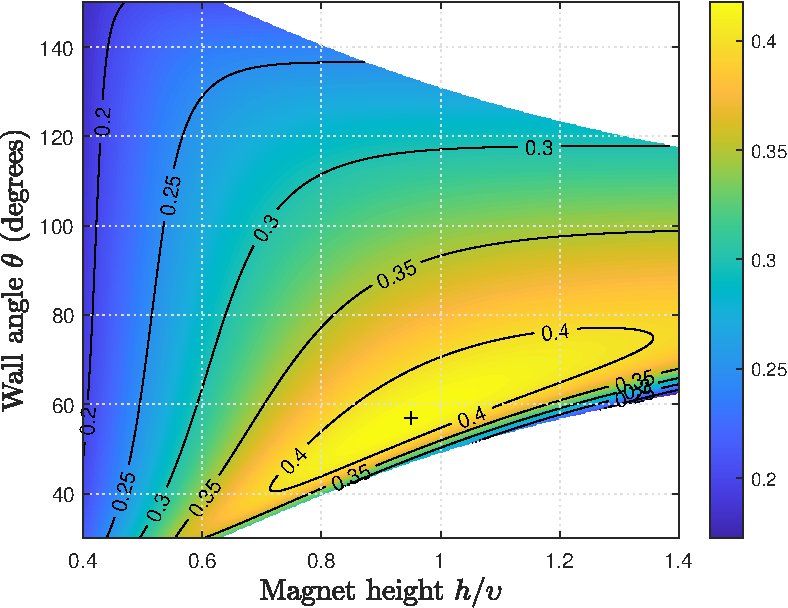
\includegraphics[width=\linewidth]{p3/p3FIG5a}
		\subcaption{}
		\label{subfig:p3centralField100}
	\end{subfigure}
	
	\begin{subfigure}{0.8\textwidth}
		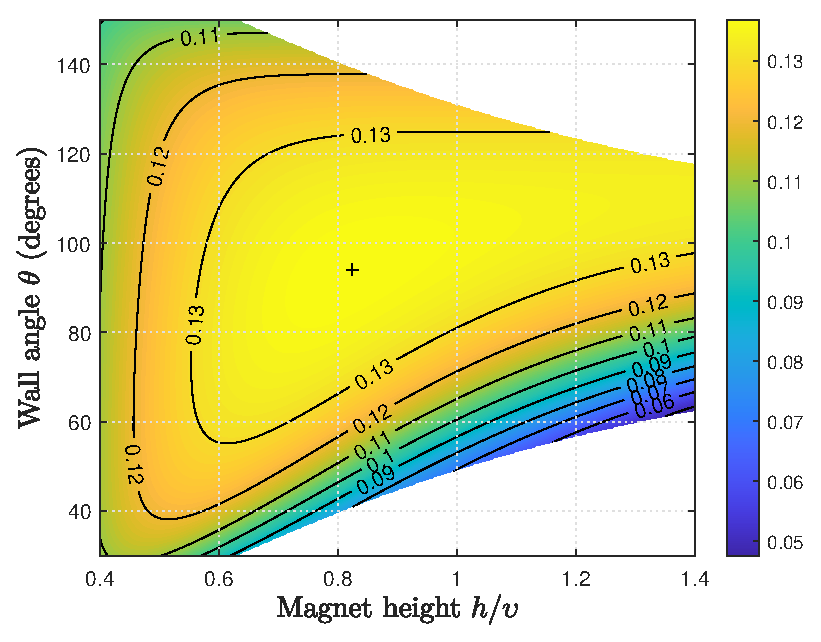
\includegraphics[width=\linewidth]{p3/p3FIG5b}
		\subcaption{}
		\label{subfig:p3centralField500}
	\end{subfigure}
	\caption{Normalised magnetic field strength \(z/\upsilon = 0.1\) (\subref{subfig:p3centralField100}) and \(z/\upsilon = 0.5\) (\subref{subfig:p3centralField500}) units above the centre of a right frustum magnet with a volume \(V\), a normalised height of \(h/\upsilon\) units and wall angle of \(\theta\) degrees. The global maxima \(\left( h_\text{opt}/\upsilon, \theta_\text{opt}\right)\) for each plot is highlighted with a `+', with the white regions indicating non-physical geometries.}
	\label{fig:p3centralField}
\end{figure}
\begin{figure}
	\centering
	

\begin{subfigure}[t]{0.45\linewidth}

\centering
\begin{tikzpicture}[scale = 0.3]

\def\LL{1}
\def\ll{4.5950}
\def\hh{5.5312}

% Define coordinates:
\coordinate(tl) at (-\LL,0);
\coordinate(tr) at (\LL,0);
\coordinate(bl) at (-\ll,-\hh);
\coordinate(br) at (\ll,-\hh);

% Draw shape
\draw (tl) -- (tr) -- (br) -- (bl) -- cycle;

% Draw dimensions
\def\hoffset{6}
\draw[<->] (-\hoffset,0) -- (-\hoffset,-\hh);
\node(h) at (-\hoffset-1.5,-2.7656) {0.951};
\draw[<->] (-\ll,-\hh-1.5) -- (\ll,-\hh-1.5);
\node(l) at (0,-\hh-2.5) {1.580};
\draw[<->] (-\LL,1.5) -- (\LL,1.5);
\node(L) at (0,2.5) {0.344};

\end{tikzpicture}

\subcaption{}
%\label{subfig:frustumschematic}

\end{subfigure}
~ \hfill ~
\begin{subfigure}[t]{0.45\linewidth}

\centering
\begin{tikzpicture}[scale = 0.3]
	
\def\LL{2.3647}
\def\ll{2.3647}
\def\hh{8.8066}

% Define coordinates:
\coordinate(tl) at (-\LL,0);
\coordinate(tr) at (\LL,0);
\coordinate(bl) at (-\ll,-\hh);
\coordinate(br) at (\ll,-\hh);

% Draw shape
\draw (tl) -- (tr) -- (br) -- (bl) -- cycle;

% Draw dimensions
\def\hoffset{5}
\draw[<->] (\hoffset,0) -- (\hoffset,-\hh);
\node(h) at (\hoffset+1.5,-4.4033) {1.514};
\draw[<->] (-\ll,-\hh-1.5) -- (\ll,-\hh-1.5);
\node(l) at (0,-\hh-2.5) {0.813};

% Draw an invisible line to centre the figure
%\draw[<->,white] (-\hoffset-2,0) -- (-\hoffset-2,-\hh);

\end{tikzpicture}

\subcaption{}
%\label{subfig:frustumschematic}

\end{subfigure}


	\caption{Normalised dimensions of the optimal frustum (left) and cuboid (right) to maximise the field for \(z/\upsilon = 0.1\). Both magnets have identical volume, but the optimal frustum has a smaller top face, which `focuses' flux, giving a slightly stronger field in the small region above the centre of the magnet.}
	\label{fig:p3optimalGeom_z_0_1}
\end{figure}
\begin{figure*}
	\centering
	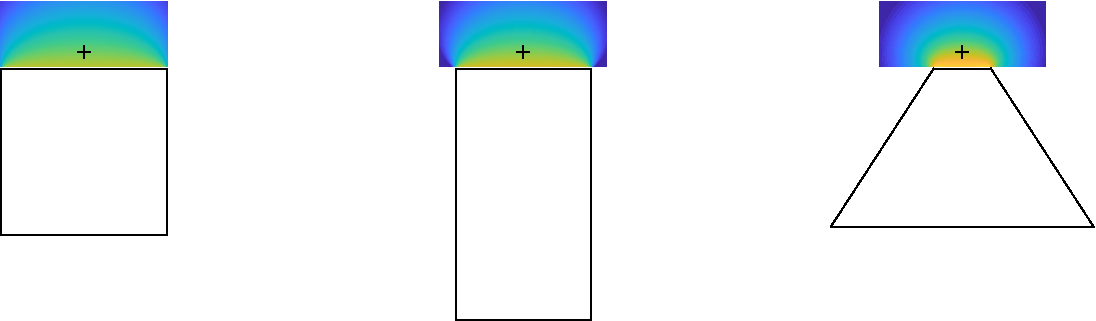
\includegraphics[width=\linewidth]{p3/p3FIG7}
	\caption{The \(z\)-field in the region above a cube magnet, the optimal cuboid magnet, and the optimal frustum magnet for \(z/\upsilon = 0.1\). The point \(z/\upsilon = 0.1\) is drawn with a `+', showing that the optimal frustum magnet gives the strongest field at this point.}
	\label{fig:p3optimalFrusAndCube}
\end{figure*}

An interior-point optimisation algorithm was used to calculate the optimal frustum geometry for a large range of distances \(z/\upsilon\) above the magnet. The optimal parameters \(h_\text{opt}/\upsilon\) and \(\theta_\text{opt}\) were calculated at each \(z/\upsilon\) and are plotted in Figure \ref{fig:p3optimalFrustumGeometry}. As \(z/\upsilon\) increases, the optimal height \(h_\text{opt}/\upsilon\) shows a decreasing trend and the wall angle \(\theta_\text{opt}\) shows an increasing trend. Interestingly, the optimal height \(h_\text{opt}/\upsilon < 1\) for all values of \(z/\upsilon\), meaning the optimal geometry is always a `flatter' magnet. The magnetic field strength for both optimal frustum and optimal cuboid are plotted in Figure \ref{fig:p3PFIeps}, along with the percentage increase in field strength using the optimal frustum rather than the optimal cuboid. This shows a negligible increase in field strength for large \(z/\upsilon\). However, for small \(z/\upsilon\), the increase in field strength may allow more effective use in applications such as magnetic power transmission, linear vibrating systems, and magnetic latching.
\begin{figure}
	\centering
	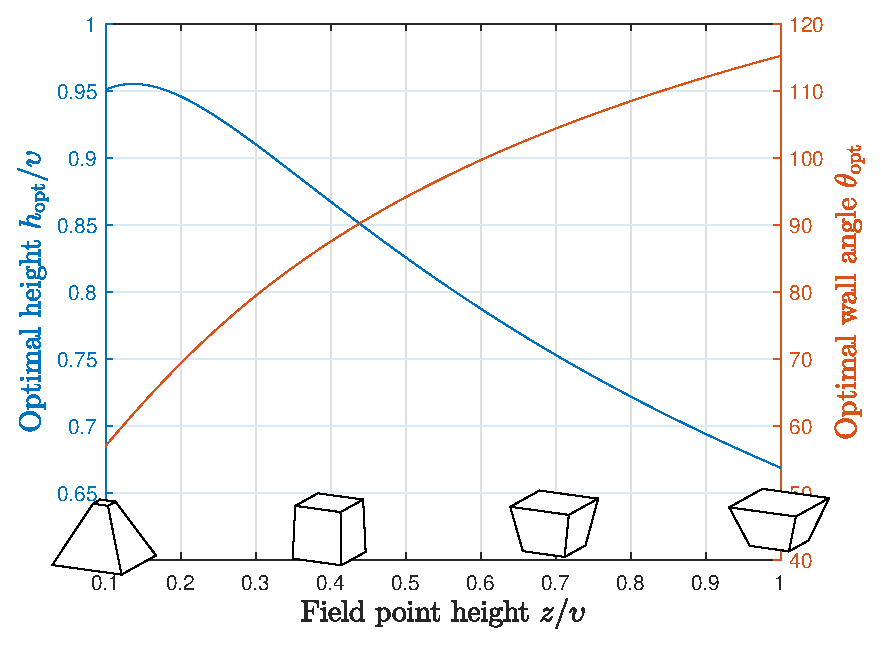
\includegraphics[width=0.8\textwidth]{p3/p3FIG8}
	\caption{Optimal frustum height \(h_\text{opt}\) (blue) and wall angle \(\theta_\text{opt}\) (orange) to maximise the magnetic field strength a distance \(z/\upsilon\) above a right frustum permanent magnet with a volume of \(V\) units\(^3\). A small image of the optimal frustum geometry is displayed at the bottom of the figure for the values \(z/\upsilon =\ \)0.1, 0.4, 0.7, and 1.0.}
	\label{fig:p3optimalFrustumGeometry}
\end{figure}
\begin{figure}
	\centering
	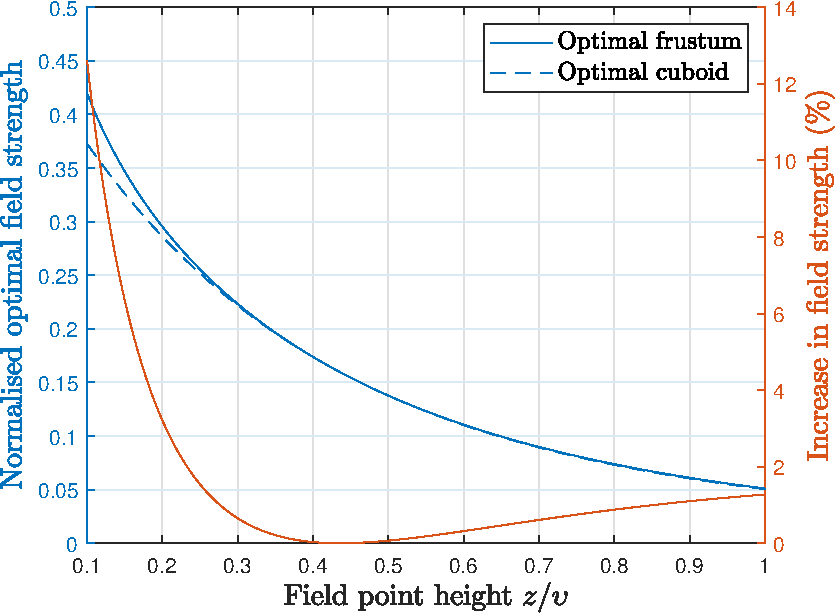
\includegraphics[width=0.8\textwidth]{p3/p3FIG9}
	\caption{Magnetic field strength produced by an optimal frustum and cuboid of the same volume (blue) and percentage increase in the field strength produced by the frustum over the cuboid (orange).}
	\label{fig:p3PFIeps}
\end{figure}
\section{Optimising the field of a planar frustum Halbach array}\label{sec:p3planarArray}
The methods detailed in this paper can also be used to analyse multi-magnet systems. This section focuses on a planar Halbach array created by tessellating frustum magnets for use in planar motors. These arrays may also be used in applications such as planar magnetic loudspeakers and 3D printers. The optimisation routine will vary the geometry to not only increase field strength, but to create a \(z\)-field which closely resembles a desired profile.

\subsection{Defining array geometry}
A planar Halbach array of frustum magnets can be created by tessellating frusta of square-based pyramids and tetrahedra, shown in Figure \ref{fig:p3halbachFrustumGeometry}. Figure \ref{fig:p3halbachFrustumGeometry} shows the repeating unit for this array, which, when duplicated, creates the array shown in Figure \ref{fig:p3planarHalbach}.
\begin{figure*}
	\centering
	\def\Lpontwo{10}
\def\lpontwo{20}
\def\Ltontwo{14}
\def\ltontwo{4}
\def\hh{25}
\def\myscale{0.07}
\def\mywidth{0.3}

\begin{subfigure}[t]{\mywidth\linewidth}

\centering
\tdplotsetmaincoords{70}{35}
\begin{tikzpicture}[scale=\myscale,tdplot_main_coords]

% Define coordinates
\coordinate(1) at (-\Lpontwo,-\Lpontwo,0);
\coordinate(2) at (\Lpontwo,-\Lpontwo,0);
\coordinate(3) at (\Lpontwo,\Lpontwo,0);
\coordinate(4) at (-\Lpontwo,\Lpontwo,0);
\coordinate(5) at (-\lpontwo,-\lpontwo,-\hh);
\coordinate(6) at (\lpontwo,-\lpontwo,-\hh);
\coordinate(7) at (\lpontwo,\lpontwo,-\hh);
\coordinate(8) at (-\lpontwo,\lpontwo,-\hh);

% Draw the shape
\draw (1) -- (2) -- (3) -- (4) -- cycle;
\draw (1) -- (5) -- (6) -- (7) -- (3);
\draw[dashed] (7) -- (8) -- (5);
\draw (2) -- (6);
\draw[dashed] (4) -- (8);

\node(Lp) at (-\Lpontwo-5,3,1) {\(L_p\)};
\node(Lp2) at (0,\Lpontwo+5,1) {\(L_p\)};
\node(lp) at (\lpontwo+5,0,-\hh-1) {\(l_p\)};
\node(lp2) at (3,-\lpontwo-6,-\hh-1) {\(l_p\)};

\end{tikzpicture}

\subcaption{}
\label{subfig:p3pfrus3d}

\end{subfigure}
~
\begin{subfigure}[t]{\mywidth\linewidth}
	
\centering
\tdplotsetmaincoords{70}{35}
\begin{tikzpicture}[scale=\myscale,tdplot_main_coords]

% Define coordinates
\coordinate(1) at (-\Ltontwo,-\Lpontwo,0);
\coordinate(2) at (\Ltontwo,-\Lpontwo,0);
\coordinate(3) at (\Ltontwo,\Lpontwo,0);
\coordinate(4) at (-\Ltontwo,\Lpontwo,0);
\coordinate(5) at (-\ltontwo,-\lpontwo,-\hh);
\coordinate(6) at (\ltontwo,-\lpontwo,-\hh);
\coordinate(7) at (\ltontwo,\lpontwo,-\hh);
\coordinate(8) at (-\ltontwo,\lpontwo,-\hh);

% Draw the shape
\draw (1) -- (2) -- (3) -- (4) -- cycle;
\draw (1) -- (5) -- (6) -- (7) -- (3);
\draw[dashed] (7) -- (8) -- (5);
\draw (2) -- (6);
\draw[dashed] (4) -- (8);

\node(Lp) at (-\Ltontwo-5,3,1) {\(L_p\)};
\node(Lt) at (0,\Lpontwo+5,1) {\(L_t\)};
\node(lp) at (\ltontwo+5,0,-\hh-1) {\(l_p\)};
\node(lt) at (3,-\lpontwo-6,-\hh-1) {\(l_t\)};

\end{tikzpicture}

\subcaption{}
\label{subfig:p3tfrus3d}
	
\end{subfigure}
~
\begin{subfigure}[t]{\mywidth\linewidth}
	
	\centering
	\tdplotsetmaincoords{70}{35}
	\begin{tikzpicture}[scale=0.06,tdplot_main_coords]
	
	% Define coordinates of z frustum
	\coordinate(1z) at (-\Lpontwo,-\Lpontwo,0);
	\coordinate(2z) at (\Lpontwo,-\Lpontwo,0);
	\coordinate(3z) at (\Lpontwo,\Lpontwo,0);
	\coordinate(4z) at (-\Lpontwo,\Lpontwo,0);
	\coordinate(5z) at (-\lpontwo,-\lpontwo,-\hh);
	\coordinate(6z) at (\lpontwo,-\lpontwo,-\hh);
	\coordinate(7z) at (\lpontwo,\lpontwo,-\hh);
	\coordinate(8z) at (-\lpontwo,\lpontwo,-\hh);
	
	% Define coordinates of x frustum
	\coordinate(1x) at (\Lpontwo,-\Lpontwo,0);
	\coordinate(2x) at (\Lpontwo+\Ltontwo+\Ltontwo,-\Lpontwo,0);
	\coordinate(3x) at (\Lpontwo+\Ltontwo+\Ltontwo,\Lpontwo,0);
	\coordinate(4x) at (\Lpontwo,\Lpontwo,0);
	\coordinate(5x) at (\lpontwo,-\lpontwo,-\hh);
	\coordinate(6x) at (\lpontwo+\ltontwo+\ltontwo,-\lpontwo,-\hh);
	\coordinate(7x) at (\lpontwo+\ltontwo+\ltontwo,\lpontwo,-\hh);
	\coordinate(8x) at (\lpontwo,\lpontwo,-\hh);
	
	% Define coordinates of y frustum
	\coordinate(1y) at (-\Lpontwo,\Lpontwo,0);
	\coordinate(2y) at (\Lpontwo,\Lpontwo,0);
	\coordinate(3y) at (\Lpontwo,\Lpontwo+\Ltontwo+\Ltontwo,0);
	\coordinate(4y) at (-\Lpontwo,\Lpontwo+\Ltontwo+\Ltontwo,0);
	\coordinate(5y) at (-\lpontwo,\lpontwo,-\hh);
	\coordinate(6y) at (\lpontwo,\lpontwo,-\hh);
	\coordinate(7y) at (\lpontwo,\lpontwo+\ltontwo+\ltontwo,-\hh);
	\coordinate(8y) at (-\lpontwo,\lpontwo+\ltontwo+\ltontwo,-\hh);
	
	% Deal with certain lines behind objects
	\draw(3y) -- (7y);
	\filldraw[fill=white] (1x) -- (2x) -- (3x) -- (4x) -- cycle;
	\filldraw[fill=white] (2x) -- (3x) -- (7x) -- (6x) -- cycle;
	
	% Draw z frustum
	\draw (1z) -- (2z);
	\draw (3z) -- (4z) -- (1z);
	\draw (1z) -- (5z) -- (6z);
	\draw (2z) -- (6z);
	
	% Draw x frustum
	\draw (5x) -- (6x);
	
	% Draw y frustum
	\draw (2y) -- (3y) -- (4y) -- (1y);
	
	% Draw an invisible node to align left and right pictures
	\node(invis) at (0,0,-1.75*\hh) { };
	
	\end{tikzpicture}
	\subcaption{}
	\label{subfig:p3subarray3d}
	
\end{subfigure}

\begin{subfigure}[t]{\mywidth\linewidth}
	
	\centering
	\begin{tikzpicture}[scale = \myscale]
	
	\coordinate(1) at (-\Lpontwo,0);
	\coordinate(2) at (\Lpontwo,0);
	\coordinate(5) at (-\lpontwo,-\hh);
	\coordinate(6) at (\lpontwo,-\hh);
	
	\draw (1) -- (2) -- (6) -- (5) -- cycle;
	\node(theta) at (-\lpontwo+3,-\hh+2.5) {\(\theta\)};
	\node(Lp) at (0,3.5) {\(L_p\)};
	\node(lp) at (0,-\hh-4) {\(l_p\)};
	\draw[<->] (\lpontwo+5,-\hh) -- (\lpontwo+5,0);
	\node(h) at (\lpontwo+7,-12.5) {\(h\)};
	
	\end{tikzpicture}
	
	\subcaption{}
	\label{subfig:p3pfrusschematic}
	
\end{subfigure}
~
\begin{subfigure}[t]{\mywidth\linewidth}
	
\centering
\begin{tikzpicture}[scale = \myscale]

\coordinate(1) at (-\Ltontwo,0);
\coordinate(2) at (\Ltontwo,0);
\coordinate(5) at (-\ltontwo,-\hh);
\coordinate(6) at (\ltontwo,-\hh);

\draw (1) -- (2) -- (6) -- (5) -- cycle;
\node(theta) at (-\Ltontwo+3,-2.5) {\(\theta\)};
\node(Lp) at (0,3.5) {\(L_t\)};
\node(lp) at (0,-\hh-4) {\(l_t\)};
\draw[<->] (\Ltontwo+5,-\hh) -- (\Ltontwo+5,0);
\node(h) at (\Ltontwo+7,-12.5) {\(h\)};

\end{tikzpicture}

\subcaption{}
\label{subfig:p3tfrusschematic}
	
\end{subfigure}
~
\begin{subfigure}[t]{\mywidth\linewidth}
	
	\centering
	\begin{tikzpicture}[scale=0.055]
	
	% Define coordinates of z frustum
	\coordinate(1z) at (-\Lpontwo,-\Lpontwo);
	\coordinate(2z) at (\Lpontwo,-\Lpontwo);
	\coordinate(3z) at (\Lpontwo,\Lpontwo);
	\coordinate(4z) at (-\Lpontwo,\Lpontwo);
	\coordinate(5z) at (-\lpontwo,-\lpontwo);
	\coordinate(6z) at (\lpontwo,-\lpontwo);
	\coordinate(7z) at (\lpontwo,\lpontwo);
	\coordinate(8z) at (-\lpontwo,\lpontwo);
	
	% Define coordinates of x frustum
	\coordinate(1x) at (\Lpontwo,-\Lpontwo);
	\coordinate(2x) at (\Lpontwo+\Ltontwo+\Ltontwo,-\Lpontwo);
	\coordinate(3x) at (\Lpontwo+\Ltontwo+\Ltontwo,\Lpontwo);
	\coordinate(4x) at (\Lpontwo,\Lpontwo);
	\coordinate(5x) at (\lpontwo,-\lpontwo);
	\coordinate(6x) at (\lpontwo+\ltontwo+\ltontwo,-\lpontwo);
	\coordinate(7x) at (\lpontwo+\ltontwo+\ltontwo,\lpontwo);
	\coordinate(8x) at (\lpontwo,\lpontwo);
	
	% Define coordinates of y frustum
	\coordinate(1y) at (-\Lpontwo,\Lpontwo);
	\coordinate(2y) at (\Lpontwo,\Lpontwo);
	\coordinate(3y) at (\Lpontwo,\Lpontwo+\Ltontwo+\Ltontwo);
	\coordinate(4y) at (-\Lpontwo,\Lpontwo+\Ltontwo+\Ltontwo);
	\coordinate(5y) at (-\lpontwo,\lpontwo);
	\coordinate(6y) at (\lpontwo,\lpontwo);
	\coordinate(7y) at (\lpontwo,\lpontwo+\ltontwo+\ltontwo);
	\coordinate(8y) at (-\lpontwo,\lpontwo+\ltontwo+\ltontwo);
	
	% Draw top plane
	\draw (1z) -- (2z) -- (3z) -- (4z) -- cycle;
	\draw (2y) -- (3y) -- (4y) -- (1y);
	\draw (1x) -- (2x) -- (3x) -- (4x);
	
	% Draw connecting planes where necessary
	\draw (1z) -- (5z);
	\draw (1x) -- (5x) -- (6x) -- (2x);
	\draw (3x) -- (7x) -- (8x) -- (4x);
	\draw (6y) -- (7y) -- (3y);
	\draw (1y) -- (5y) -- (8y) -- (4y);
	
	% Draw bottom plane
	\draw (8z) -- (5z) -- (6z);
	\draw[dashed] (6z) -- (7z) -- (8z);
	\draw[dashed] (7y) -- (8y);
	\draw[dashed] (6x) -- (7x);
	
	% Draw some dimensions
	\draw[<->] (-\Lpontwo,-\lpontwo-5) -- (\Lpontwo,-\lpontwo-5);
	\draw[<->] (\Lpontwo,-\lpontwo-5) -- (\Lpontwo+2*\Ltontwo,-\lpontwo-5);
	\draw[<->] (-\lpontwo-5,-\lpontwo) -- (-\lpontwo-5,\lpontwo);
	\draw[<->] (-\lpontwo-5,\lpontwo) -- (-\lpontwo-5,\lpontwo+2*\ltontwo);
	\node(Lp) at (0,-\lpontwo-10) {\(L_p\)};
	\node(Lt) at (\Lpontwo+\Ltontwo,-\lpontwo-10) {\(L_t\)};
	\node(lp) at (-\lpontwo-9,0) {\(l_p\)};
	\node(lt) at (-\lpontwo-9,\lpontwo+\ltontwo) {\(l_t\)};
	
	\end{tikzpicture}
	\subcaption{}
	\label{subfig:p3subarrayschematic}
	
\end{subfigure}


	\caption{Three dimensional views and schematics of a pyramid frustum (\subref{subfig:p3pfrus3d},\subref{subfig:p3pfrusschematic}), a tetrahedral frustum (\subref{subfig:p3tfrus3d},\subref{subfig:p3tfrusschematic}), and the repeating unit (\subref{subfig:p3subarray3d},\subref{subfig:p3subarrayschematic}).}
	\label{fig:p3halbachFrustumGeometry}
\end{figure*}
\begin{figure}
	\centering
	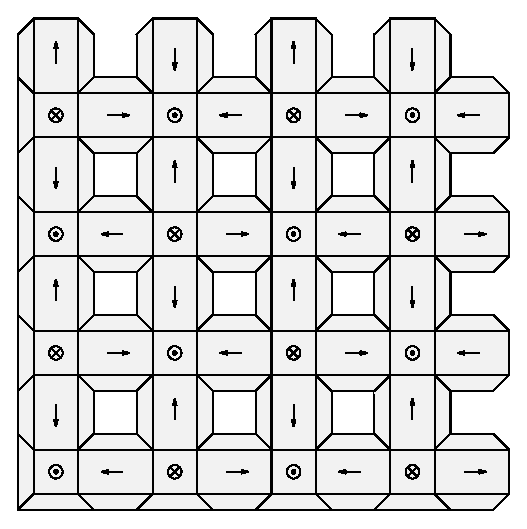
\includegraphics[width=0.7\linewidth]{p3/p3FIG11}
	\caption{Planar Halbach array created by replicating the magnetic subarray from Figure \ref{fig:p3halbachFrustumGeometry}. The pyramid frusta have magnetisations in the \(z\)-direction (into and out of the page), whereas the tetrahedral frusta have magnetisations in the \(x\)- and \(y\)-directions (parallel to the page).}
	\label{fig:p3planarHalbach}
\end{figure}

The square-based pyramid frustum (Figure \ref{fig:p3squareFrustum}) requires three parameters to fully describe its geometry, while the tetrahedral frustum requires five parameters, totalling eight parameters. However, for the magnets to tessellate, two of the length parameters (\(l_p\) and \(L_p\)), the wall angle \(\theta\), and height \(h\) are shared between the two, leaving only four parameters required to fully describe the system geometry. This is reduced to two parameters by keeping the system volume and pole pitch \(\tau\) constant.

Consider the repeating unit shown in Figure \ref{fig:p3halbachFrustumGeometry} (\subref{subfig:p3subarray3d} and \subref{subfig:p3subarrayschematic}) with the magnets having an average volume \(V\). Let the total volume of the three magnets be \(3V\) units\(^3\) and the pole pitch be \(\tau = L_p + L_t = l_p + l_t\) units. Define the parameters \(h\) and \(\theta\) as variables. Thus, the geometry is fully defined by the relations
\begin{align}
l_p &= \tau + h \cot \theta - S \\ 
L_p &= \tau - h \cot \theta - S \\
l_t &= -h \cot \theta + S \\
L_t &= h \cot \theta + S \text{,}
\end{align}
where
\begin{equation}
S = \sqrt{\tau^2 - \frac{3V}{h} - \frac{h^2}{3} \cot^2\theta} \text{.}
\end{equation}
Therefore, for constant \(V\) and \(\tau\), the array geometry can be fully described using the variables \(h\) and \(\theta\).

\subsection{Optimisation of field for a specific case}\label{sec:p3specificOptimisation}
Consider an array using a repeating unit with length \(\tau/\upsilon = 2\) for use in a planar motor with low force ripple and large maximum force. Selection of a suitable desired field profile depends on coil geometry specific to each motor, but this work considers only permanent magnet geometry, and as such a general sinusoidal profile is chosen as the desired \(z\)-field profile. Further extensions of this work could consider a field profile tailored to a particular motor design. Although force ripple will not be completely removed using a sinusoidal profile, it will be reduced when compared to the field produced by a traditional cuboidal array. In addition, a field profile with a large amplitude will lead to a larger maximum force for the motor. Thus, a sinusoid with large amplitude is chosen as the desired field profile for the optimisation routine. Both the resemblance and amplitude can be quantified using a least squares analysis on calculated field data and the appropriate two-dimensional cosine wave \(f\), given by
\begin{equation}\label{eqn:p3cosineWave}
f\left(x,y\right) = A\cos\left(\frac{\pi x}{\tau}\right)\cos\left(\frac{\pi y}{\tau}\right) \text{,}
\end{equation}
where \(A\) is the amplitude of the sinusoid.

For a given geometry \(\left(h/\upsilon,\theta\right)\) and vertical distance \(z/\upsilon\) from the array, the \(z\)-field was calculated over a \(2\tau/\upsilon\times2\tau/\upsilon\) region across a \(32\times32\) grid of points to include one full wavelength of the magnetic field. This calculation was done using five pole pitches in each direction, giving a large enough array such that end effects were negligible, but maintaining a relatively small calculation time. At each point, \(f\) was calculated, and the sum of squared residuals minimised to give the value of the wave amplitude \(A\). The coefficient of determination \(r^2\) was calculated, giving a measure of similarity between the field data and cosine wave. This process was repeated for a large range of geometries \(\left(\theta, h/\upsilon\right)\), and contour plots drawn for \(r^2\) and \(A\). These plots show the optimal regions to maximise \(r^2\) or \(A\), and are shown for \(z/\upsilon = 0.2\) in Figure \ref{fig:p3planarHalbachData}.
\begin{figure}
	\centering
	\begin{subfigure}{0.8\textwidth}
		\centering
		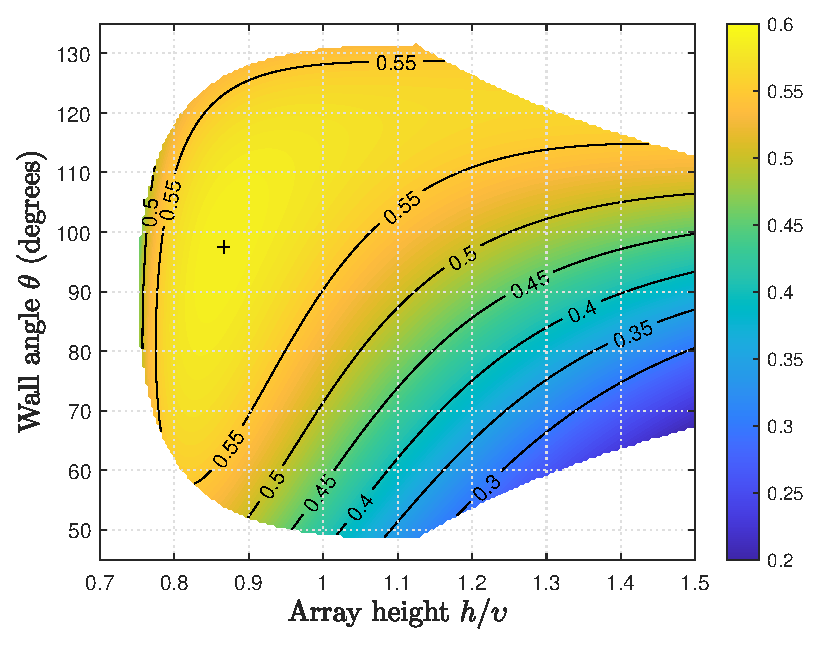
\includegraphics[width=\linewidth]{p3/p3FIG12a}
		\subcaption{}
		\label{subfig:p3planarHalbach_amp}
	\end{subfigure}
	
	\vfill
	
	\begin{subfigure}{0.8\textwidth}
		\centering
		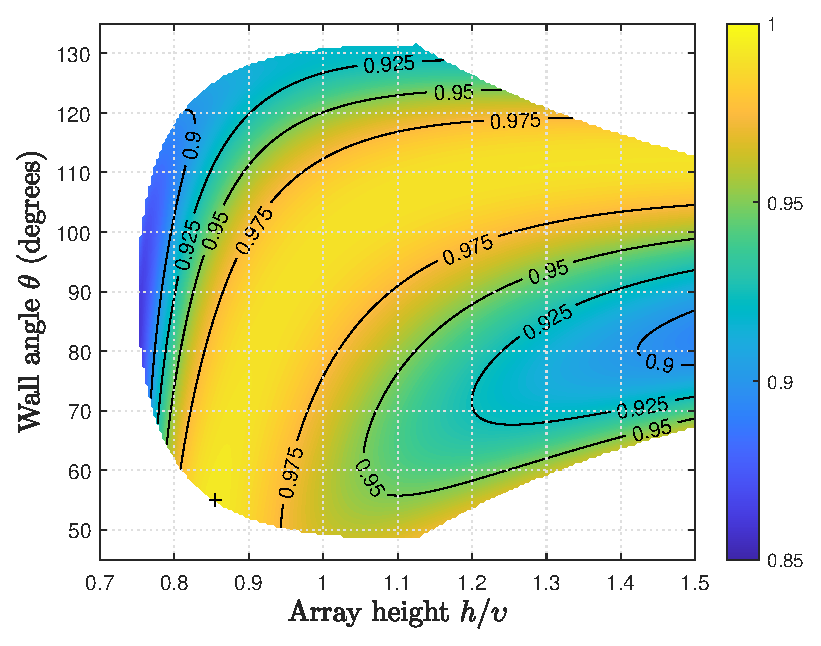
\includegraphics[width=\linewidth]{p3/p3FIG12b}
		\subcaption{}
		\label{subfig:p3planarHalbach_rsq}
	\end{subfigure}
	\caption{Normalised amplitude \(A\) (\subref{subfig:p3planarHalbach_amp}) and coefficient of determination \(r^2\) (\subref{subfig:p3planarHalbach_rsq}) of the cosine wave approximation of the \(z\)-field above the planar magnet array with \(\tau/\upsilon=2\) and \(z/\upsilon = 0.2\). The global maxima are plotted with a `+', with the white region indicating non-physical geometries.}
	\label{fig:p3planarHalbachData}
\end{figure}

The contour plots indicated that there are relatively large regions which maximise \(r^2\) and \(A\). The region to maximise \(r^2\) is a curved stripe, starting with low \(\theta\) and \(h/\upsilon\), passing through the cube case (\(\theta = \) \ang{90}, \(h/\upsilon = 1\)), and tending toward large \(\theta\) and \(h/\upsilon\). The region to maximise \(A\) is a triangular area in the top left of the plot. There is overlap between the optimal regions of both plots along the bottom edge of the optimal region of \(A\) and the top edge of the optimal region of \(r^2\). Hence, the geometry to maximise both \(r^2\) and \(A\) will be in this overlap region.

This can be further examined by defining a cost function to maximise both,
\begin{equation}\label{eqn:p3CostFunction}
C = Ar^2 \text{.}
\end{equation}

Maximising \(C\) will give large values for both \(r^2\) and \(A\), thereby obtaining a field which closely resembles a cosine wave with large amplitude. The cost function \(C\) was calculated at each combination \(\left(\theta, h/\upsilon\right)\) (Figure \ref{fig:p3planarHalbach_wavequality}). This plot shows a region coinciding with the overlap of Figures \ref{subfig:p3planarHalbach_rsq} and \ref{subfig:p3planarHalbach_amp} as expected. The maximum value of this plot occurs at \(h_\text{opt}/\upsilon = 0.89\) and \(\theta_\text{opt} =\) \ang{93.3}. This geometry is almost cuboidal, and thus corresponds to an increase of only 0.04\% in \(C\) over the optimal cuboidal geometry.
\begin{figure}
	\centering
	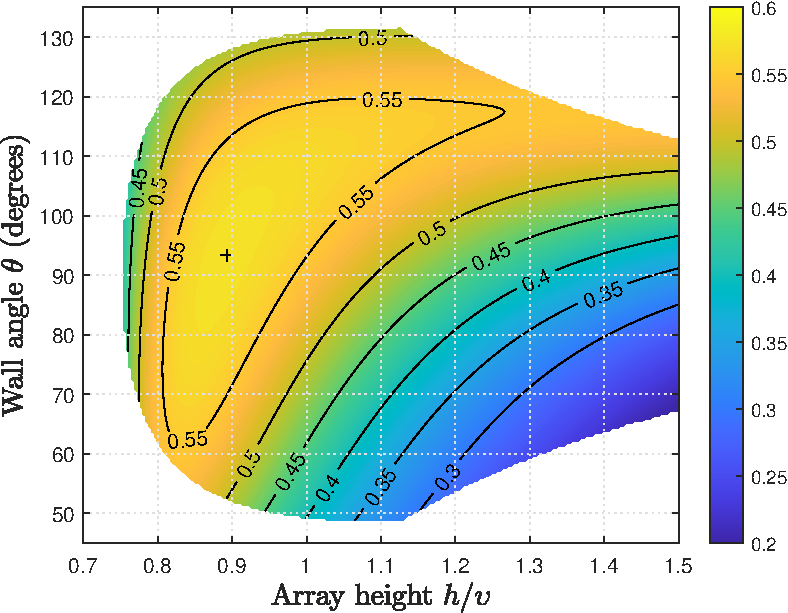
\includegraphics[width=0.8\linewidth]{p3/p3FIG13}
	\caption{The value of the cost function \(C = Ar^2\) at each point in the physically realisable region with \(\tau/\upsilon=2\) and \(z/\upsilon = 0.2\). This value is maximised in the top-left area of the region, with optimal parameters of \(h_\text{opt}/\upsilon = 0.89\) and \(\theta_\text{opt} = \) \ang{93.3}.}
	\label{fig:p3planarHalbach_wavequality}
\end{figure}

\subsection{Optimisation of field for a general case}
The methodology outlined in Section \ref{sec:p3specificOptimisation} can be extended to consider more general cases. However, rather than evaluating the value of \(C\) at each feasible geometry \(\left( \theta, h/\upsilon \right)\), an optimisation routine is used, substantially reducing the number of evaluations of \(C\). Additionally, all length parameters can be normalised by \(z\), allowing a nondimensional analysis, leading to a more general solution.

A range of values were defined for \(\upsilon/z\) and \(\tau/z\), and limits on geometries imposed to discard geometries with extreme aspect ratios. For each combination \(\left( \upsilon/z, \tau/z\right)\), the region of physically realisable geometries was identified in terms of \(h/z\) and \(\theta\). The Matlab function \texttt{fmincon} was then used to maximise the cost function \(C\) over the physically realisable magnet geometries \(\left(\theta, h/z\right)\). This process was repeated for each combination \(\left( \upsilon/z, \tau/z\right)\), and the results plotted on the contour plots in Figure \ref{fig:p3optvalues}, with the corresponding value of the cost function \(C\) plotted in Figure \ref{fig:p3generalPlanarHalbachQuality}.
\begin{figure}
	\centering
	\begin{subfigure}{0.8\textwidth}
		\centering
		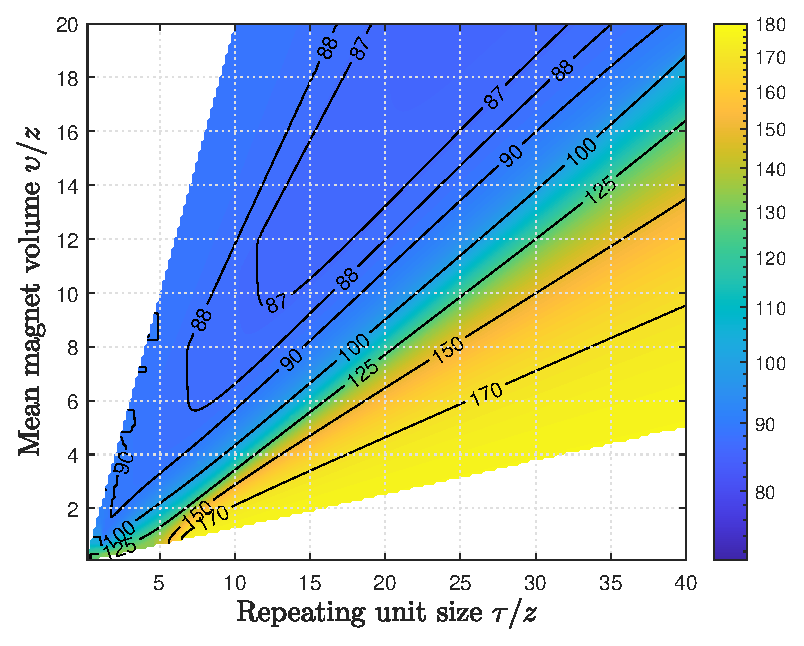
\includegraphics[width=\linewidth]{p3/p3FIG14a}
		\subcaption{}
		\label{subfig:p3opttheta}
	\end{subfigure}
	
	\begin{subfigure}{0.8\textwidth}
		\centering
		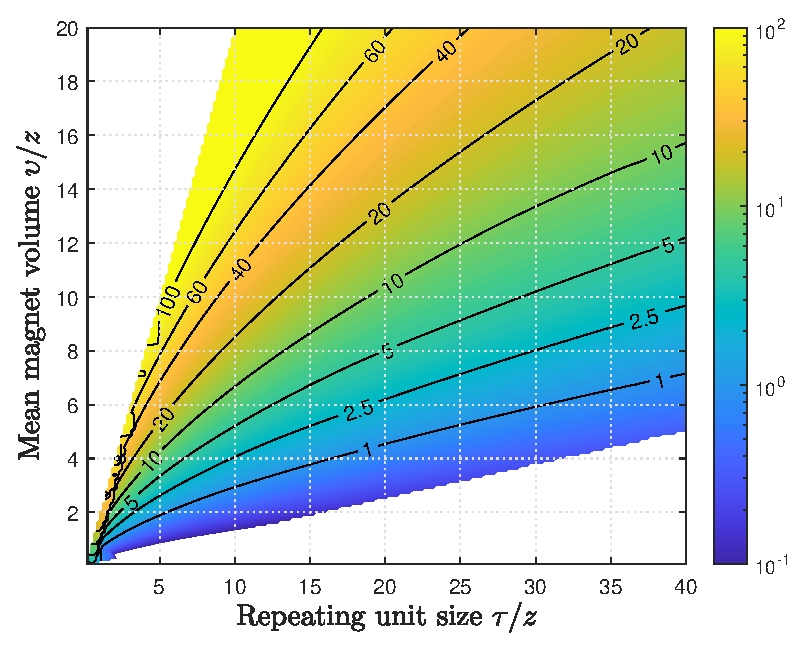
\includegraphics[width=\linewidth]{p3/p3FIG14b}
		\subcaption{}
		\label{subfig:p3opth}
	\end{subfigure}
	\caption{The optimal value of \(\theta\) (\subref{subfig:p3opttheta}) and \(h/z\) (\subref{subfig:p3opth}) for a given combination \(\left( \upsilon/z, \tau/z \right)\). The white regions indicate magnet topologies with undesirable aspect ratios.}
	\label{fig:p3optvalues}
\end{figure}
\begin{figure}
	\centering
	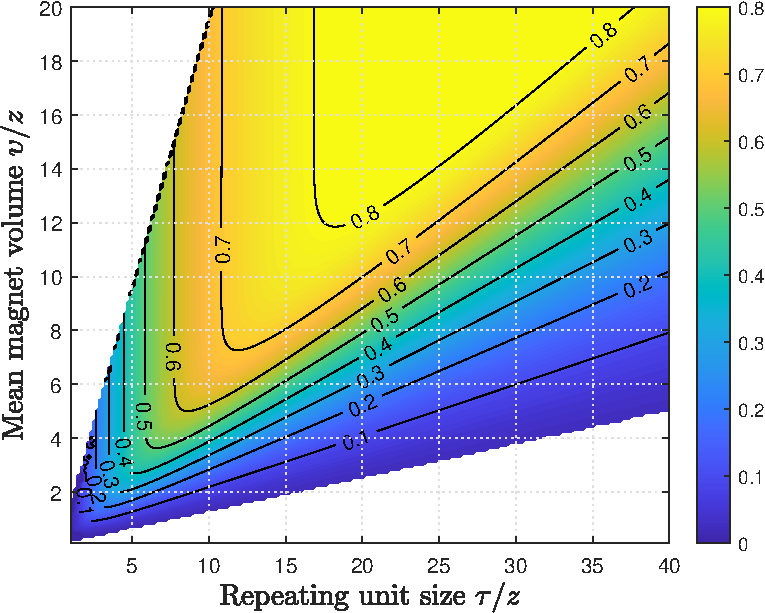
\includegraphics[width=0.8\linewidth]{p3/p3FIG15}
	\caption{The value of the cost function \(C = Ar^2\) at each combination \(\left( \upsilon/z, \tau/z \right)\) normalised by the magnetisation strength of the magnets. This value approaches unity for large \(\tau/z\) and \(\upsilon/z\), and becomes small when either \(\tau/z\) or \(\upsilon/z\) are small.}
	\label{fig:p3generalPlanarHalbachQuality}
\end{figure}

Interestingly, the upper half of the plots indicate a magnet geometry close to a cuboid. However, as the volume decreases or pole pitch increases, the optimal angle \(\theta\) grows larger, leading to a highly non-cuboidal geometry. The optimal height parameter behaves as would be expected, with increasing height as the volume increases or pole pitch decreases.

The optimal frustum topologies can be directly compared to the corresponding cuboidal topologies. The optimisation routine was run again, but this time only optimising the height parameter while maintaining the angle \(\theta\) at \ang{90}. The cost function \(C_\text{cuboid}\) was calculated and compared to the associated frustum cost function \(C\). The percentage increase in \(C\) produced by the optimal frustum over optimal cuboid was plotted for each combination \(\left( \upsilon/z, \tau/z \right)\) and is shown in Figure \ref{fig:p3percentageIncrease}, showing a small but nonzero increase in field quality.
\begin{figure}
	\centering
	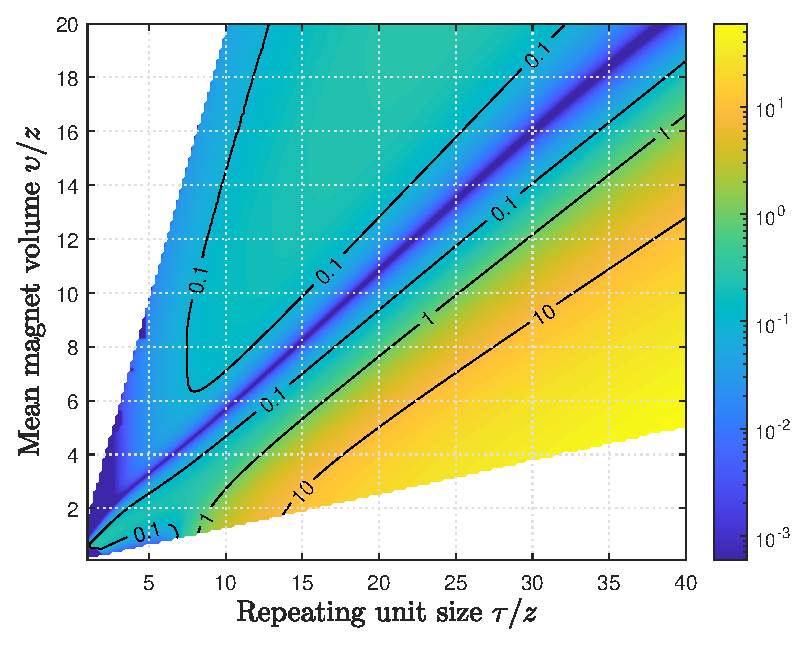
\includegraphics[width=0.8\linewidth]{p3/p3FIG16}
	\caption{Percentage increase in the cost function \(C\) using optimal frustum magnets rather than optimal cuboid magnets. In the centre of the region, the percentage increase is extremely small, implying no effective increase in performance using optimal frusta instead of optimal cuboids. In some regions, this percentage increase is larger. However, these are regions where the cost function is relatively small whether using frusta or cuboids, so it is likely more effective to redesign the system than to optimise magnet geometry.}
	\label{fig:p3percentageIncrease}
\end{figure}

In most of the region, this increase is less than 1 percent, meaning the increased difficulty and cost associate with manufacturing frustum magnets rather than cuboidal magnets is likely not worth the small increase in \(C\). The bottom right region of the plot shows a more considerable percentage increase, achieving an increase greater than 10\%. However, there are two main issues with this region. Firstly, the magnets will exhibit an extremely undesirable aspect ratio. Based on Figure \ref{subfig:p3opth}, this region has a relatively small optimal height parameter \(h/z\) in a region with large \(\tau/z\), leading to a large value of \(\tau/h\) and an undesirable aspect ratio of the magnets. Secondly, this region attains a relatively low value of \(C\) according to Figure \ref{fig:p3generalPlanarHalbachQuality}. This is partially because the magnets are very thin due to the large value of \(\tau/h\), leading to weak fields, and partially because the ratio \(\tau/z\) is large, leading to the field resembling a square wave rather than a sinusoid. These tendencies lead to a small field amplitude \(A\), with a low coefficient of determination \(r^2\), leading to a small value of \(C\).

Based on Figure \ref{fig:p3percentageIncrease}, optimal frustum magnets are likely not worth the additional difficulty and cost associated with manufacturing and assembly for a planar Halbach array. The increase in field amplitude and resemblance to a sinusoid are negligible in most regions. In the region where the increase is not insignificant, the amplitude and resemblance to a sinusoid are small independent of the magnet shape. In this region, it is likely better to redesign the system to increase the magnet volume or decrease the pole pitch of the array. In general, optimal cuboidal magnets are likely the most effective solution for a planar Halbach array which aims to attain a sinusoidal magnetic field with a large amplitude.
\section{Conclusion}\label{sec:p3conclusion}
This paper has examined the differences in the magnetic field produced by frustum permanent magnets and cuboidal permanent magnets. This was done by applying magnetic field equations currently available in literature \cite{OConnell2020a} to a six-faced frustum geometry. Two magnetic systems were considered, allowing a direct comparison between cuboidal magnets and six-faced frustum magnets.

The first magnetic system consisted of a single magnet, with the field being computed at a point directly above the centre of the magnet. In this case, it was shown that an optimised frustum magnet can produce a field stronger than that of an optimised cuboid magnet. However, this increase in field strength is only significant when the field point is close to the magnet. As the field point moves further from the magnet, this increase becomes negligible.

The second magnetic system was a two-dimensional Halbach array consisting of tessellated frustum magnets. For this configuration, the amplitude of the field and how closely the field represents a two-dimensional sinusoid defined a cost function \(C\) (to be maximised), which was used to optimise the system. It was found that most optimal frustum geometries were close to cuboidal. As a comparison, the optimal cuboidal arrays were found, showing that in most cases, the optimal frustum topology has negligible effect on the cost function \(C\). Under certain conditions, the optimal frustum array leads to a significant increase in \(C\) over the optimal cuboid array. However, these conditions lead to a relatively weak field, and other measures should be taken to increase \(C\) such as increasing magnet volume or decreasing the array pole pitch.

This paper shows that although frustum magnets can produce more desirable magnetic fields than cuboidal magnets, this effect is insignificant in many cases. Additionally, complicated magnet geometries such as frusta are more expensive to produce than simple geometries such as cuboids. Hence, the cost associated with the manufacture of these magnets is likely not worth the advantage of a more desirable field. Measures such as varying magnet volume and size are likely to be more effective than using complicated magnet geometries. Furthermore, for multi-magnet arrays, optimising magnet topology and magnetisations is likely more effective than varying the geometry of individual magnets.
\clearpage
\section*{Author's remarks on Chapter \ref{chap:paper3}}
This chapter demonstrated the optimisation of both a singular magnet and a planar array of magnets. For the singular magnet case, the geometry was varied to maximise the magnetic field strength at a point above the centre of the magnet. In the case of the planar magnet array, the array geometry was varied to maximise a cost function associated with the magnetic field above the array. The cost function chosen was a simple two-dimensional sinusoidal pattern, but the choice of cost function has a strong dependence on the application being optimised. Therefore, the results presented in this chapter may not be optimal for every application, but give an indication of the subspace of where the optimal geometry may be. Due to the complexity of the optimisation problem in this chapter, fast field calculation methods such as detailed in Chapter \ref{chap:paper2} were necessary to achieve a solution to the problem in a reasonable time. This chapter has shown a proof of concept in magnetostatic geometry optimisation using efficient field calculations.

\newpage
\section*{References}
\addcontentsline{toc}{section}{\protect\numberline{}References}
\printbibliography[heading=none]
\chapter{Modelling permeable magnets}\label{chap:paper4}
\fancyhead[LE]{\scshape Chapter\ \ref{chap:paper4}}
While the methodologies presented in previous chapters are fast and accurate, they are based on idealised permanent magnets with the assumption of a relative permeability of unity. However, most modern permanent magnet materials have a relative permeability in the range of 1.05--1.3, leading to a small overestimation in the fields, forces, and torques associated with these magnets. To minimise this overestimation, magnetic permeability must be incorporated into the magnetic model. Past literature has explored the effect of magnetic permeability, but this is usually done through an iterative method, in which the field is calculated several times. This chapter presents and validates a methodology to solve a magnetic system without iteration. Specifically, the field is calculated only once, with a matrix inversion performed to solve for the magnetic surface charges, allowing the calculation of the fields, forces, and torques. Validation is performed using finite element simulations, but assumes non-unity relative permeability.
%\subsection*{Statement of authorship}
\renewcommand{\arraystretch}{1.5}
\begin{tabular}{m{0.25\textwidth} m{0.67\textwidth}}
    \hline \hline Paper title & A non-iterative method to solve for magnetic fields, forces, and torques due to permanent magnets with non-unity relative permeability \\ \hline
    Publication status & Submitted \\ \hline
    Publication details & Submitted to \textit{Journal of Magnetism and Magnetic Materials}, Dec. 2021 \\ \hline \hline
\end{tabular}

\vfill

\subsection*{Principal author}
\begin{tabular}{p{0.25\textwidth} m{0.67\textwidth}}
    \hline \hline Name & James O'Connell \\ \hline
    Contribution & \begin{itemize}
        \setlength\itemsep{-2mm}\small
        \item[-] Idea conceptualisation
        \item[-] Review of relevant literature
        \item[-] Deriving a matrix equation for the surface charge density of a magnet based on the field present and the remanence magnetisation of the magnet
        \item[-] Incorporating Gauss' Law for Magnetism into the system
        \item[-] Applying a constrained least squares methodology to solve an overdetermined matrix equation with constraints
        \item[-] Adapting the system of equations to include an arbitrary number of magnetic bodies and arbitrary external magnetic fields
        \item[-] Applied the surface charge density solution to find the magnetic field at any point
        \item[-] Applied the surface charge density solution to estimate the force and torque imparted on all magnets in the system
        \item[-] Implemented the surface charge, magnetic field, force, and torque methodologies in MATLAB code
        \item[-] Created finite element simulations to verify the algorithms and MATLAB code
        \item[-] Analysed the accuracy of the methodology based on mesh density
        \item[-] Wrote manuscript draft and created all figures
        \item[-] Finalisation of article
        \item[-] Preparation and submission for publication, including author correspondence
    \end{itemize} \\ \hline
    Percentage & 90\% \\ \hline
    Certification & \small This paper reports on original research conducted by the author during the period of Higher Degree by Research candidature and is not subject to any obligations or contractual agreements with a third party that would constrain its inclusion in this thesis. The author listed above is the primary author of this paper. \\ \hline
    Signature & \begin{tabular}{m{45mm} m{10mm} m{20mm}}
    \vspace{0.5mm}\includegraphics[width=0.3\textwidth]{jamesSignature.PNG} & Date: & 8 Dec 2021
    \end{tabular}
\end{tabular}

\vfill
    
\subsection*{Co-author contributions}
By signing this statement of authorship, each author certifies that:
\begin{enumerate}
    \item the candidate's stated contribution to the publication is accurate (as detailed above);
    \item permission is granted for the candidate to include the publication in the thesis; and
    \item the sum of all co-author contributions is equal to 100\% less the candidate's stated contribution.
\end{enumerate}
\begin{tabular}{m{0.25\textwidth} m{0.67\textwidth}}
    \hline \hline Name & Will Robertson \\ \hline
    Contribution & 5\% \\ \hline
    Signature & \vspace{2mm}\includegraphics[height=10mm]{willSig} \\  \hline
    Date & 16 Dec 2021 \\
    \hline \hline Name & Ben Cazzolato \\ \hline
    Contribution & 5\% \\ \hline
    Signature & \vspace{2mm} \includegraphics[height=10mm]{benSig} \\ \hline
    Date & 16 Dec 2021 \\
    \hline \hline \vfill
\end{tabular}
\renewcommand{\arraystretch}{1}
\newpage
%
\section*{\LARGE A non-iterative method to solve for magnetic fields, forces, and torques due to permanent magnets with non-unity relative permeability}
James L.G. O'Connell, William S.P. Robertson, and Benjamin S. Cazzolato
\section*{Abstract}\addcontentsline{toc}{section}{\protect\numberline{}Abstract}\label{sec:p4abstract}
Although the majority of common permanent magnet materials have relative permeabilities between 1.05 and 1.3, they are often modelled analytically with the assumption of unity relative permeability. While this greatly simplifies analysis, it introduces modelling errors, leading to overestimates of magnetic fields, forces, and torques. This paper presents a new method for modelling interactions between magnets with non-unity relative permeabilities assuming constant uniform remanence magnetisation and permeability. In contrast to other methods which use an iterative approach, this methodology requires calculating magnetic field information only once, leading to a considerable reduction in computational effort. Based on a triangular surface mesh, this method permits the calculation for any magnetic geometry and for magnetic systems with arbitrarily many magnets. Verification is performed using finite element simulations, with the proposed method showing high accuracy and speed.
\section{Introduction}\label{sec:p4introduction}
Magnetic materials are used in many applications found in science and engineering, including electric motors, loudspeakers, and magnetic data storage. Each material has a given magnetic relative permeability \(\mu_r\), which describes how the magnetisation of the material changes when magnetic fields are present. Most permanent magnet materials have a relative permeability slightly larger than unity, but are often modelled with \(\mu_r = 1\), ignoring the effect of permeability. This significantly decreases the complexity of modelling, but introduces errors as the magnitude of permeability increases. Some materials such as iron have a high permeability, and are often modelled by assuming the permeability is infinite, also leading to modelling errors. To reduce these modelling errors, non-unity finite permeability must be considered, but this is difficult to model and analyse, often requiring the use of finite element simulations or iterative solvers.

Several researchers have attempted to analytically model magnetic permeability with varying levels of success. \textcite{Kremers2013} modelled a permanent magnet with non-unity permeability by modifying the magnetisation strength of the magnet based on the permeability. This approach gives extremely fast results for the magnetic field produced by a single magnet with low permeability. However, it does not consider the effect of external fields or magnets, and is only valid for small and constant permeabilities, limiting accuracy. \textcite{Dam2016} extended upon this by calculating the interaction force in two of the three Cartesian directions as one magnet is rotated with non-unity relative permeability. However, the third force component was not derived, and the methodology is only valid for cuboidal magnets. \textcite{Casteren2014} published a more general iterative methodology applicable to any magnet geometry, which was more accurate at the cost of considerably longer calculation times. Their approach assumed constant permeability and required recalculating the magnetic field for each iteration, but could incorporate external fields and arbitrarily large permeabilities. In a recent study, \textcite{Zhang2021} performed a similar analysis by subdividing cuboidal permanent magnets into a large number of smaller cuboidal magnets, with the magnetisation of each augmented by the effects of permeability. The force equations from \textcite{Akoun1984}, which assume unity relative permeability, were implemented on each small cuboid, giving accurate force calculations which incorporate the effect of permeability. \textcite{Forbes2021} also subdivided magnetic materials into smaller volumes of material with similar outcomes. Provided the permeability of each segment remains uniform across its volume, the permeability within each sub-volume was able to vary, allowing the modelling of nonlinear magnetic materials.

\textcite[Sec~2.6]{Harrington1993} presented an interesting methodology in electrostatics, wherein the polarisability of a dielectric body is calculated under the assumption of non-unity relative electric permittivity. This is analogous to finding the magnetisation of a magnetic body with non-unity relative permeability, but in the electrostatic domain rather than the magnetostatic. Their method is based on solving a matrix equation based on electric surface charges and the permittivity of the material, allowing a solution to be found. However, their method uses approximations of the integral equations for the field, leading to small but non-trivial errors in the solution.

The current paper introduces a new methodology for calculating magnetic fields, forces, and torques due to magnetic materials with non-unity permeabilities in a single step, thus avoiding iteration. It is similar in concept to the aforementioned matrix equation given by \textcite[Sec~2.6]{Harrington1993}, but with several advantages. The method presented in this paper uses the exact solution to the field equations, leading to high accuracy. In addition, a constraint is applied to the system to ensure consistency with Gauss' Law for Magnetism, further increasing accuracy. Furthermore, systems with arbitrarily many magnets and systems with external field sources may be analysed with this method. Finally, the methodology presented in this paper includes the evaluation of forces and torques on magnetic bodies through numeric integration, allowing analysis of quasi-static magnetic systems.

This methodology is extremely fast and gives accurate results for any magnet shape due to the use of a triangular surface mesh. The methodology begins by calculating surface charge densities in Section \ref{sec:p4magneticChargeDensity}, before using these results to calculate magnetic fields (Section \ref{sec:p4magneticField}), as well as forces and torques (Section \ref{sec:p4forceAndTorque}). Verification is performed on this methodology using several magnetic configurations in Section \ref{sec:p4verification}. Finally, computational considerations are detailed in Section \ref{sec:p4computationalPerformance} before the paper is concluded.
\section{Magnetic charge density}\label{sec:p4magneticChargeDensity}
To calculate the effect of magnetic permeability on magnetic materials, this paper uses the magnetic charge model \cite{Furlani2001}, where fictitious magnetic charges exist on the surface of and inside magnetic bodies. An example of this is depicted in Figure \ref{fig:p4singleMagnetPicture}, where an idealised permanent magnet with unity relative permeability \(\mu_r = 1\) and a non-ideal permanent magnet with \(\mu_r = 3\) have been drawn, with positive charges shown in red and negative charges in blue. Both magnets have identical remanence magnetisations, but the non-ideal magnet has a demagnetising effect on itself due to a relatively large value of permeability, resulting in weaker surface charges and some charges migrating from the north and south poles to the sides of the magnet. For non-unity relative permeability, the distributions of magnetic charge on the magnet surfaces is unknown and must be solved based on their interaction with each other and any applied magnetic field. This section outlines an approach to calculating these charge densities which uses a one-step matrix inversion rather than the iterative approach commonly seen in literature.
\begin{figure}
    \centering
    \begin{subfigure}{0.7\textwidth}
        \centering
        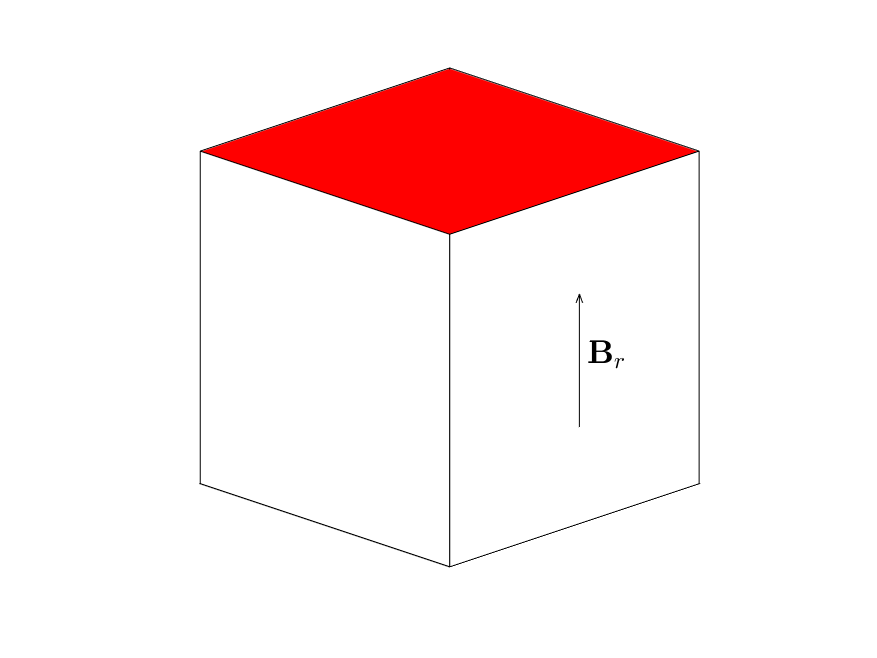
\includegraphics[width=\linewidth]{p4/p4FIG1a}
        \caption{}\label{fig:p4singleMagnetIdealised}
    \end{subfigure}
    \begin{subfigure}{0.7\textwidth}
        \centering
        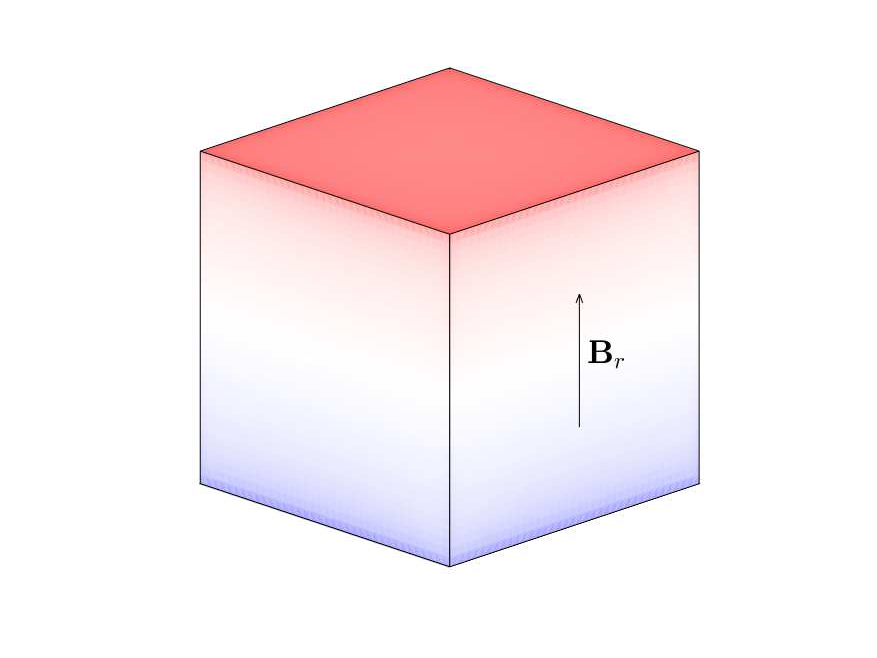
\includegraphics[width=\linewidth]{p4/p4FIG1b}
        \caption{}\label{fig:p4singleMagnetNonideal}
    \end{subfigure}
    \caption{A cube magnet with an ideal relative permeability \(\mu_r = 1\) (a) and a non-ideal relative permeability \(\mu_r = 3\) (b). The remanence magnetisation of both magnets is equal in strength and in the vertical direction, with the associated surface charges shown in red (positive charge) and blue (negative charge). The surface charges on the idealised magnet (\(\mu_r = 1\)) remain on the poles, whereas the charges on the non-ideal magnet (\(\mu_r = 3\)) migrate from the poles and become weaker due to the self-demagnetising effect of relatively large permeability.}
    \label{fig:p4singleMagnetPicture}
\end{figure}
%
\subsection{Induced magnetisation and surface charge density}
At any point in space, magnetic materials satisfy the constitutive relationship
\begin{equation}\label{eqn:p4constitutiveRelation}
    \mathbf{B} = \mu_0 \left( \mathbf{H} + \mathbf{M} \right)
\end{equation}
and Gauss' law for magnetism
\begin{equation}\label{eqn:p4gaussLawForMagnetism}
    \oiint_S \mathbf{B} \cdot d\mathbf{s}' \text{,}
\end{equation}
where \(\mathbf{B}\) is the magnetic flux density, \(\mu_0\) is the permeability of free space, \(\mathbf{H}\) is the magnetic field intensity, \(\mathbf{M}\) is the magnetisation of the material, and \(S\) is any closed surface in space. In addition, if the material is linear with a constant permeability \(\mu\), the flux density follows
\begin{equation}\label{eqn:p4linearMaterial}
    \mathbf{B} = \mu \mathbf{H} + \mathbf{B}_r \text{,}
\end{equation}
where \(\mathbf{B}_r\) is the remanence magnetisation of the material.

Combining Equations (\ref{eqn:p4constitutiveRelation}) and (\ref{eqn:p4linearMaterial}) leads to the equivalent magnetisation
\begin{equation}\label{eqn:p4equivalentMagnetisation}
    \mathbf{M} = \frac{1}{\mu} \mathbf{B}_r + \frac{\mu_r - 1}{\mu} \mathbf{B} \text{,}
\end{equation}
where \(\mu_r = \mu / \mu_0\) is the relative permeability of the material (with magnetic susceptibility \(\chi = \mu_r - 1\)). Thus, if the magnetic flux density is calculated and the remanence magnetisation known, the equivalent magnetisation can be calculated.

To solve Equation (\ref{eqn:p4equivalentMagnetisation}), an expression for the magnetic flux density \(\mathbf{B}\) must be found. Here, the magnetic charge model is used due to its accuracy and simplicity, but a number of other methods may be used. The magnetic flux density produced by a volume \(V\) bounded by a surface \(S\) at a location \(\mathbf{x}\) is presented by \textcite{Furlani2001} (pp. 132),
\begin{align}\label{eqn:p4chargeModel}
    \mathbf{B}\left( \mathbf{x} \right) = \frac{\mu_0}{4\pi} & \left( \oiint_{S} \left( \mathbf{M} \cdot \hat{\mathbf{n}} \right) \frac{\mathbf{x} - \mathbf{x}'}{\left| \mathbf{x} - \mathbf{x}' \right|^3} \ ds' - \iiint_{V} \left( \nabla \cdot \mathbf{M} \right) \frac{\mathbf{x} - \mathbf{x}'}{\left| \mathbf{x} - \mathbf{x}' \right|^3} \ dv' \right) \text{,}
\end{align}
where \(\mathbf{M}\) is the magnetisation of the volume, \(\hat{\mathbf{n}}\) is the outward-facing unit normal vector of the surface \(S\), and \(\mathbf{x}'\) is a point on \(S\) or in \(V\).

If each volume \(V\) is assumed to have constant uniform remanence magnetisation and constant permeability, \(\nabla \cdot \mathbf{M} = 0\) (Appendix \ref{sec:p4noVolumeCharge}) and the volume integral in Equation (\ref{eqn:p4chargeModel}) disappears, leaving the simplified charge model
\begin{align}\label{eqn:p4simplifiedChargeModel}
    \mathbf{B}\left( \mathbf{x} \right) = \frac{\mu_0}{4\pi} \oiint_{S} \sigma \left( \mathbf{x}' \right) \frac{\mathbf{x} - \mathbf{x}'}{\left| \mathbf{x} - \mathbf{x}' \right|^3} \ ds' \text{,}
\end{align}
where \(\sigma = \mathbf{M} \cdot \hat{\mathbf{n}}\) is the magnetic surface charge density.

Combining Equations (\ref{eqn:p4equivalentMagnetisation}) and (\ref{eqn:p4simplifiedChargeModel}) gives the equivalent magnetisation
\begin{equation}\label{eqn:p4badMagnetisationEquation}
    \mathbf{M} = \frac{1}{\mu} \mathbf{B}_r + \frac{\mu_r - 1}{\mu} \frac{\mu_0}{4\pi} \oiint_{S} \sigma \left( \mathbf{x}' \right) \frac{\mathbf{x} - \mathbf{x}'}{\left| \mathbf{x} - \mathbf{x}' \right|^3} \ ds' \text{.}
\end{equation}
To more easily analyse the system, a scalar equation may be employed using the scalar surface charge density rather than the magnetisation vector field. The equivalent surface charge density \(\sigma \left( \mathbf{x} \right)\) can be found by calculating the dot product of Equation (\ref{eqn:p4badMagnetisationEquation}) and the outward-facing unit normal vector \(\hat{\mathbf{n}}\),
\begin{align}\label{eqn:p4analyticSigma}
    \sigma \left( \mathbf{x} \right) = \frac{1}{\mu_r} \sigma_r + \frac{\mu_r - 1}{\mu} \frac{\mu_0}{4\pi} \oiint_{S} \sigma \left( \mathbf{x}' \right) \frac{\mathbf{x} - \mathbf{x}'}{\left| \mathbf{x} - \mathbf{x}' \right|^3} \ ds' \cdot \hat{\mathbf{n}} \text{,}
\end{align}
where \(\sigma_r = \mathbf{B}_r/\mu_0 \cdot \hat{\mathbf{n}}\) is defined as the remanence surface charge density.

Solving \(\sigma\) using Equation (\ref{eqn:p4analyticSigma}) is difficult, because \(\sigma\) is present both inside and outside of the integral. This problem suggests an iterative approach to solving \(\sigma\), such as in \cite{Casteren2014}. However, this issue can be avoided by applying a surface mesh to \(S\), as is shown in the following sections.

\subsection{Surface mesh}
By applying a surface mesh with \(N\) elements to \(S\), each surface element can be considered separately with its own surface charge density. When applied to a surface \(S\), Equation (\ref{eqn:p4gaussLawForMagnetism}) implies that (Appendix \ref{sec:p4integralSigma})
\begin{equation}
    \oiint_S \sigma \left(\mathbf{x}\right) ds = 0 \text{.}
\end{equation}
After meshing the surface and assuming that \(\sigma_i\) is constant across each surface, we obtain
\begin{equation}\label{eqn:p4sumOfSigmaEquation}
    \sigma_1 a_1 + \sigma_2 a_2 + \dots + \sigma_N a_N = 0 \text{,}
\end{equation}
where \(a_i\) is the area of the \(i\)th surface element. If Equation (\ref{eqn:p4sumOfSigmaEquation}) is false, the net magnetic charge of the system is non-zero, leading to inconsistency with Gauss' law. Thus, Equation (\ref{eqn:p4sumOfSigmaEquation}) will form a constraint on the solution of the magnetic system.

In addition, applying Equation (\ref{eqn:p4analyticSigma}) to the element \(i\) results in the definition of the surface charge density of each element \(\sigma_i\) as
\begin{align}
    \sigma_i \left( \mathbf{x}_i \right) &= \frac{1}{\mu_r} \sigma_{ir}\ + \frac{\mu_r - 1}{\mu} \sum_j \frac{\mu_0}{4\pi} \iint_{S_j} \sigma_j \left( \mathbf{x}_j' \right) \frac{\mathbf{x}_i - \mathbf{x}_j'}{\left| \mathbf{x}_i - \mathbf{x}_j' \right|^3} \ ds_j' \cdot \hat{\mathbf{n}}_i \text{,}
\end{align}
where \(\sigma_{ir}\) is the remanence surface charge density of element \(i\), \(\mathbf{x}_i\) is a point on element \(i\), and \(S_j\) is the surface of element \(j\).

If the surface mesh is chosen such that the surface charge density is approximately constant over each element, then \(\sigma_j \left( \mathbf{x}_j \right) \approx \sigma_j\), which can then be moved outside the integral,
\begin{align}\label{eqn:p4analyticSigmaDiscretised}
    \sigma_i \approx & \frac{1}{\mu_r} \sigma_{ir} + \frac{\mu_r - 1}{\mu} \sum_j \frac{\mu_0}{4\pi} \sigma_j \iint_{S_j} \frac{\mathbf{x}_i - \mathbf{x}_j'}{\left| \mathbf{x}_i - \mathbf{x}_j' \right|^3} \ ds_j' \cdot \hat{\mathbf{n}}_i \ \text{.}
\end{align}
The accuracy of each \(\sigma_i\) calculation increases as the mesh density increases. In addition, if a triangular surface mesh is used, any polyhedral geometry can be analysed this way, and curved surfaces may be approximated by a polyhedral surface with a large number of elements. This allows an accurate analysis of any magnetic geometry.

To simplify Equation (\ref{eqn:p4analyticSigmaDiscretised}), \(\hat{B}_{ij}\) is defined as
\begin{equation}\label{eqn:p4Bij}
    \hat{B}_{ij} = \frac{\mu_0}{4\pi} \iint_{S_j} \frac{\mathbf{x}_i - \mathbf{x}_j'}{\left| \mathbf{x}_i - \mathbf{x}_j' \right|^3} \ ds_j' \cdot \hat{\mathbf{n}}_i \text{,}
\end{equation}
which is equal to the normal magnetic flux density produced by element \(j\) at the centre of element \(i\) due to a unit surface charge density. The integral has been solved for triangular and trapezial elements by the current authors in a previous publication \cite{OConnell2020a}, and can be dot multiplied with the outward-facing normal vector to give \(\hat{B}_{ij}\). Note that to most efficiently calculate the force and torque in Section \ref{sec:p4forceAndTorque}, it is best to calculate the integral and store the result in \(\hat{B}_{xij}\), \(\hat{B}_{yij}\), and \(\hat{B}_{zij}\), before calculating the dot product. Substituting Equation (\ref{eqn:p4Bij}) into Equation (\ref{eqn:p4analyticSigmaDiscretised}) leads to 
\begin{equation}\label{eqn:p4sigmaApprox}
    \sigma_i \approx \frac{1}{\mu_r} \sigma_{ir} + \frac{\mu_r - 1}{\mu} \sum_j \hat{B}_{ij} \sigma_j \text{.}
\end{equation}

Equations (\ref{eqn:p4sumOfSigmaEquation}) and (\ref{eqn:p4sigmaApprox}) can be used to construct a matrix form of the problem, allowing the solution of all surface charge densities simultaneously. 

\subsection{Matrix equations}
It can be seen that Equations (\ref{eqn:p4sumOfSigmaEquation}) and (\ref{eqn:p4sigmaApprox}) represent a set of linear equations. Thus, we can write these equations as a set of matrix equations to manipulate and solve more easily. To do this, a vector of surface charge densities with length \(N\) is defined by
\begin{equation}
    \bm{\sigma} = \begin{bmatrix} \sigma_1 \\ \sigma_2 \\ \vdots \\ \sigma_N \end{bmatrix}
\end{equation}
with a similar vector of element surface areas given by
\begin{equation}
    \mathbf{a} = \begin{bmatrix} a_1 & a_2 & \dots & a_N \end{bmatrix} \text{,}
\end{equation}
Equation (\ref{eqn:p4sumOfSigmaEquation}) simplifies to
\begin{equation}\label{eqn:p4gaussLawMatrixEquation}
    \mathbf{a} \bm{\sigma} = 0 \text{.}
\end{equation}

To reduce Equation (\ref{eqn:p4sigmaApprox}) to a matrix equation, a matrix \(\hat{B}\) is defined by
\begin{equation}
    \hat{B} = \begin{bmatrix} \hat{B}_{11} & \hat{B}_{12} & \dots & \hat{B}_{1N} \\
    \hat{B}_{21} & \hat{B}_{22} & \dots & \hat{B}_{2N} \\
    \vdots & \vdots & \ddots & \vdots \\
    \hat{B}_{N1} & \hat{B}_{N2} & \dots & \hat{B}_{NN} \end{bmatrix} \nonumber \text{,}
\end{equation}
along with the remanence surface charge density vector,
\begin{equation}
    \bm{\sigma}_0 = \begin{bmatrix} \sigma_{1r} \\ \sigma_{2r} \\ \vdots \\ \sigma_{Nr} \end{bmatrix} \text{.}
\end{equation}
Thus, equation (\ref{eqn:p4sigmaApprox}) becomes the matrix equation
\begin{equation}\label{eqn:p4preIterativeEquation}
    \bm{\sigma} \approx K \bm{\sigma}_0 + J \hat{B} \bm{\sigma} \text{,}
\end{equation}
where
\begin{equation}
    K = \frac{1}{\mu_r}
\end{equation}
and
\begin{equation}
    J = \frac{\mu_r - 1}{\mu} \text{.}
\end{equation}
Assuming the matrix
\begin{equation}\label{eqn:p4CEquation}
    C = I - J \hat{B}
\end{equation}
is invertible (Appendix \ref{sec:p4invertibleMatrix}), where \(I\) is the \(\left(N\times N\right)\) identity matrix, Equation (\ref{eqn:p4preIterativeEquation}) can be rearranged to solve for all surface charge densities,
\begin{equation}\label{eqn:p4sigma}
    \bm{\sigma} \approx C ^{-1} K \bm{\sigma}_0 \text{.}
\end{equation}

Here, we have obtained an \(\left(N \times N\right)\) approximate matrix equation for the \(N\) surface charge densities in Equation (\ref{eqn:p4sigma}), with the constraint in Equation (\ref{eqn:p4gaussLawMatrixEquation}). This suggests using the method of constrained least squares, where
\begin{equation}
    \left| C\bm{\sigma} - K \bm{\sigma}_0 \right|^2
\end{equation}
is minimised, subject to the constraint \(\mathbf{a}\bm{\sigma} = 0\). This is done using the \( \left( N+1 \right) \times \left( N+1 \right)\) matrix equation
\begin{equation}
    \begin{bmatrix} 2C^\mathsf{T}C & \mathbf{a}^\mathsf{T} \\ \mathbf{a} & 0 \end{bmatrix} \begin{bmatrix} \bm{\sigma} \\ z \end{bmatrix} = \begin{bmatrix} 2C^\mathsf{T} K \bm{\sigma}_0 \\ 0 \end{bmatrix} \text{.}
\end{equation}
Thus, an accurate approximation for the surface charge densities which satisfy Gauss' Law for Magnetism is given by the first \(N\) elements of the solution to
\begin{equation}\label{eqn:p4singleMagnetSolution}
     \begin{bmatrix} \bm{\sigma} \\ z \end{bmatrix} = \begin{bmatrix} 2C^\mathsf{T}C & \mathbf{a}^\mathsf{T} \\ \mathbf{a} & 0 \end{bmatrix}^{-1} \begin{bmatrix} 2C^\mathsf{T} K \bm{\sigma}_0 \\ 0 \end{bmatrix} \text{.}
\end{equation}

While it is possible to simply solve Equation (\ref{eqn:p4sigma}) for the surface charge densities without the inclusion of Gauss' law, doing so often leads to a non-zero net surface charge density for the system. This is inconsistent with Gauss' law, and often leads to unbalanced forces and torques, violating Newton's third law. Since the inclusion of Gauss' law adds insignificant computation effort, it is beneficial to solve the constrained least squares problem given in Equation (\ref{eqn:p4singleMagnetSolution}) to ensure consistency with Maxwell's equations and improve accuracy of the final calculations.

\subsection{Multi-magnet systems}
In the previous sections, it is assumed that although the surface charge density \(\sigma_i\) of every element can vary, each element shares the same permeability \(\mu\). However, many magnetic systems consist of multiple magnetic objects, each with differing permeabilities. In this case, a small extension can be made to Equation (\ref{eqn:p4singleMagnetSolution}), allowing the calculation of the surface charge densities of magnetic objects with differing permeabilities. If \(J\) and \(K\) are redefined as the diagonal matrices
\begin{equation}\label{eqn:p4JEquation}
	J = \begin{bmatrix} \frac{\mu_{r1} - 1}{\mu_1} & 0 & \cdots & 0 \\
	0 & \frac{\mu_{r2} - 1}{\mu_2} & \cdots & 0 \\
	\vdots & \vdots & \ddots & \vdots \\
	0 & 0 & \cdots & \frac{\mu_{rN} - 1}{\mu_N} \end{bmatrix}
\end{equation}
and
\begin{equation}\label{eqn:p4KEquation}
	K = \begin{bmatrix} \frac{1}{\mu_{r1}} & 0 & \cdots & 0 \\
	0 & \frac{1}{\mu_{r2}} & \cdots & 0 \\
	\vdots & \vdots & \ddots & \vdots \\
	0 & 0 & \cdots & \frac{1}{\mu_{rN}} \end{bmatrix} \text{,}
\end{equation}
where \(\mu_n\) and \(\mu_{rn}\) are the permeability and relative permeability of element \(n\) respectively, the matrix \(C\) may be recalculated.

Once \(C\) is recalculated, Equation (\ref{eqn:p4singleMagnetSolution}) may be solved, but we can impose further constraints to yield a more accurate solution. Rather than applying Gauss' Law for Magnetism to the entire system, it can be applied to each magnet individually, giving one constraint per magnet. Given a system with \(M\) magnets, the area vector \(_m\mathbf{a}\) may be defined as
\begin{equation}
    _m\mathbf{a} = \begin{bmatrix} _ma_1 & _ma_2 & \dots \end{bmatrix} \text{,}
\end{equation}
where \(_ma_1\) is the area of the first element of magnet \(m\), \(_ma_2\) is the area of the second element of magnet \(m\), and so on. These area vectors may be formed into an \(M \times N\) block diagonal matrix \(A\), given by
\begin{equation}\label{eqn:p4AEquation}
    A = \begin{bmatrix} _m\mathbf{a} & \bm{0} & \bm{0} & \dots & \bm{0} \\
    \bm{0} & _2\mathbf{a} & \bm{0} & \dots & \bm{0} \\
    \bm{0} & \bm{0} & _3\mathbf{a} & \dots & \bm{0} \\
    \vdots & \vdots & \vdots & \ddots & \vdots \\
    \bm{0} & \bm{0} & \bm{0} & \dots & _M\mathbf{a} \end{bmatrix} \text{,}
\end{equation}
where each \(\bm{0}\) is a zero-values row vector. Applying Gauss' Law for Magnetism to each magnet in the system gives the new constraint
\begin{equation}
    A\bm{\sigma} = \bm{0} \text{.}
\end{equation}
This may be incorporated into the constrained least squares system, giving the solution to the \(\left(M+N\right)\times\left(M+N\right)\) linear system
\begin{equation}\label{eqn:p4multiMagnetSolution}
    \begin{bmatrix} \bm{\sigma} \\ z \end{bmatrix} = \begin{bmatrix} C^\mathsf{T}C & A^\mathsf{T} \\ A & 0 \end{bmatrix}^{-1} \begin{bmatrix} C^\mathsf{T} K \bm{\sigma}_0 \\ 0 \end{bmatrix} \text{.}
\end{equation}

One considerable advantage of this methodology is that the surface charges of several magnetic bodies may be solved simultaneously. Here, there is no need to calculate the effect of magnet 2 on magnet 1, then magnet 3 on magnet 1, and so on. Rather, the information of all magnetic bodies is encapsulated in the constrained least squares system, and the surface charge densities of the entire system may be solved with a single matrix inversion.

\subsection{External fields}\label{sec:p4externalFields}
Thus far in the derivation, only the fields generated by the magnetic bodies themselves have been considered; fields generated by other sources such as an electromagnetic coil or the Earth have not been incorporated. However, the methodology can be adapted to include these effects. The normal component of the external field \(\mathbf{B}_\text{ext}\) may be calculated at the centre of element \(n\) by calculating the dot product of the field at that point and the outward-facing unit normal vector, and is denoted by \(B_{\text{norm},n}\). An \(\left(N\times 1\right)\) vector can be defined by concatenating these normal field components, giving the vector of normal external fields,
\begin{equation}
    \mathbf{B}_\text{ext,norm} = \begin{bmatrix} B_{\text{norm},1} \\ B_{\text{norm},2} \\ \vdots \\ B_{\text{norm},N} \end{bmatrix} \text{.}
\end{equation}
This can be incorporated into the constrained least squares, giving the solution
\begin{equation}\label{eqn:p4externalMultiMagnetSolution}
    \begin{bmatrix} \bm{\sigma} \\ z \end{bmatrix} = \begin{bmatrix} C^\mathsf{T}C & A^\mathsf{T} \\ A & 0 \end{bmatrix}^{-1} \begin{bmatrix} C^\mathsf{T} \left( K \bm{\sigma}_0 + J\mathbf{B}_\text{ext,norm} \right) \\ 0 \end{bmatrix} \text{,}
\end{equation}
with \(J\), \(K\), \(C\), and \(A\) being defined by Equations (\ref{eqn:p4JEquation}), (\ref{eqn:p4KEquation}), (\ref{eqn:p4CEquation}), and (\ref{eqn:p4AEquation}) respectively.

\subsection{Summary}
This section has outlined a methodology for calculating the surface charge densities of magnetic surface elements assuming each element has a constant permeability and constant uniform remanence magnetisation. A surface mesh is applied to each magnetic body in a system, and a large matrix \(\hat{B}\) is defined. The \(\left(i,j\right)\) entry of \(\hat{B}\) is given by the normal component of the magnetic flux density at the centre of element \(i\) due to element \(j\), assuming element \(j\) has unity charge density. In addition, a vector \(\bm{\sigma}_0\) is defined as the initial surface charge densities of each element, diagonal matrices \(J\) and \(K\) initialised containing permeability information, and a block diagonal matrix \(A\) defined containing the area of each element. Finally, the surface charges \(\bm{\sigma}\) are solved using Equation (\ref{eqn:p4externalMultiMagnetSolution}). These surface charges are used in the following sections to calculate magnetic fields (Section \ref{sec:p4magneticField}), as well as forces and torques (Section \ref{sec:p4forceAndTorque}).
\section{Magnetic field calculation}\label{sec:p4magneticField}
Once the magnetic surface charges \(\bm{\sigma}\) are known, the magnetic field can be calculated using the magnetic charge model. The magnetic field \(\mathbf{B}\) at the point \(\mathbf{x}\), assuming constant permeability and remanence magnetisation, is given by
\begin{equation}
	\mathbf{B}\left( \mathbf{x} \right) = \frac{\mu_0}{4\pi} \oiint_{S} \sigma \left( \mathbf{x}' \right) \frac{\mathbf{x} - \mathbf{x}'}{\left| \mathbf{x} - \mathbf{x}' \right|^3} \ ds' \text{.}
\end{equation}
As above, the surface can be discretised and the surface charge term moved outside the integral to give an approximate solution,
\begin{equation}
	\mathbf{B}\left( \mathbf{x} \right) \approx \sum_i \frac{\mu_0}{4\pi} \sigma_i \iint_{S_i} \frac{\mathbf{x} - \mathbf{x}_i'}{\left| \mathbf{x} - \mathbf{x}_i' \right|^3} \ ds_i' \ \text{.}
\end{equation}
A \(3 \times N\) matrix \(B\) is defined as
\begin{equation}
    \hat{B} = \begin{bmatrix} \hat{\mathbf{B}}_1 & \hat{\mathbf{B}}_2 & \cdots & \hat{\mathbf{B}}_N \end{bmatrix} \text{,}
\end{equation}
where the columns are given by
\begin{equation}
	\hat{\mathbf{B}}_i\left(\mathbf{x}\right) = \frac{\mu_0}{4\pi} \iint_{S_i} \frac{\mathbf{x} - \mathbf{x}_i'}{\left| \mathbf{x} - \mathbf{x}_i' \right|^3} \ ds_i' \text{.}
\end{equation}
Here, \(\hat{B}\) is the magnetic flux density at the point \(\mathbf{x}\) due to every surface element having unity surface charge density. This can again be calculated using previously published equations from the current authors \cite{OConnell2020a}. Using this matrix, the field at \(\mathbf{x}\) is given by
\begin{equation}
	\mathbf{B}\left(\mathbf{x}\right) \approx \hat{B} \left(\mathbf{x}\right) \bm{\sigma} \text{.}
\end{equation}
If an external field is present, given by the \(3\times 1\) vector \(\mathbf{B}_\text{ext}\), this can simply be added to the field produced by the system, giving
\begin{equation}
    \mathbf{B}\left(\mathbf{x}\right) \approx \hat{B} \left(\mathbf{x}\right) \bm{\sigma} + \mathbf{B}_\text{ext}\left(\mathbf{x}\right) \text{,}
\end{equation}
where \(\mathbf{B}_\text{ext}\left(\mathbf{x}\right)\) is the external magnetic field at the point \(\mathbf{x}\).
\section{Force and torque}\label{sec:p4forceAndTorque}
In addition to the magnetic field, the force and torque on each magnet can be approximated using the surface charge densities. According to the magnetic charge model described by \textcite{Furlani2001} (pp. 136,142), the force and torque on a magnetic body are given respectively by
\begin{equation}
	\mathbf{F} = \iiint_V \rho \mathbf{B}_\text{ext} \ dv + \oiint_S \sigma \mathbf{B}_\text{ext} \ ds
\end{equation}
and
\begin{equation}
	\mathbf{T} = \iiint_V \rho \left( \mathbf{r} \times \mathbf{B}_\text{ext} \right) \ dv + \oiint_S \sigma \left( \mathbf{r} \times \mathbf{B}_\text{ext} \right) \ ds \text{,}
\end{equation}
where \(\rho\) and \(\sigma\) are the volume and surface charge densities of the magnetic body respectively, \(\mathbf{B}_\text{ext}\) is the external magnetic field (including the field generated by other magnetic bodies in the system), and \(\mathbf{r}\) is the vector from the point about which the torque is calculated.

Under the assumptions of constant uniform remanence magnetisation and constant permeability, the volume integrals disappear, leaving only the surface integrals. These equations can be applied to the surface mesh defined earlier, giving equations for the approximate force and torque on magnet \(m\).

To achieve this, the vector of surface charge densities \(\bm{\sigma}\) is split into a vector of charge densities of the surface elements of magnet \(m\), \({}_m\bm{\sigma}\), and all other surface charge densities, \({}_{\overline{m}}\bm{\sigma}\). Similarly, the vector from the centre of each element of magnet \(m\) to the point about which the torque is to be calculated is defined as \({}_m\mathbf{r}\). Submatrices \(\hat{B}^*_x\), \(\hat{B}^*_y\), and \(\hat{B}^*_z\) are constructed by taking the rows corresponding to elements belonging to magnet \(m\) and the columns corresponding to elements not belonging to magnet \(m\) of the matrices \(\hat{B}_x\), \(\hat{B}_y\), and \(\hat{B}_z\) respectively. \({}_m\mathbf{B}_{\text{ext,}x}\), \({}_m\mathbf{B}_{\text{ext,}y}\), and \({}_m\mathbf{B}_{\text{ext,}z}\) are defined as the magnetic field at the centre of each surface element of magnet \(m\) produced by external sources such as coils. In the following equations, the operator \(\odot\) is defined as the Hadamard (element-wise) product of two vectors. If the total field on each element produced by all other magnets and the external field is defined as
\begin{align*}
    _m\mathbf{B}_x &= \hat{B}^*_x\ {}_{\overline{m}}\bm{\sigma} + {}_m\mathbf{B}_{\text{ext,}x} \text{,} \\
    _m\mathbf{B}_y &= \hat{B}^*_y\ {}_{\overline{m}}\bm{\sigma} + {}_m\mathbf{B}_{\text{ext,}y} \text{,} \\
    _m\mathbf{B}_z &= \hat{B}^*_z\ {}_{\overline{m}}\bm{\sigma} + {}_m\mathbf{B}_{\text{ext,}z} \text{,}
\end{align*}
the force and torque on magnet \(m\) can be approximated as
\begin{align}
	_mF_x &\approx \left( {}_m\bm{\sigma} \odot {}_m\mathbf{a} \right)^\mathsf{T} {}_m\mathbf{B}_x \text{,} \\
	_mF_y &\approx \left( {}_m\bm{\sigma} \odot {}_m\mathbf{a} \right)^\mathsf{T} {}_m\mathbf{B}_y \text{,} \\
	_mF_z &\approx \left( {}_m\bm{\sigma} \odot {}_m\mathbf{a} \right)^\mathsf{T} {}_m\mathbf{B}_z \text{,}
\end{align}
and
\begin{align}
	_mT_x &\approx \left( {}_m\bm{\sigma} \odot {}_m\mathbf{a} \right)^\mathsf{T} \left( {}_m\mathbf{r}_y \odot {}_m\mathbf{B}_z - {}_m\mathbf{r}_z \odot {}_m\mathbf{B}_y \right) \text{,} \\
	_mT_y &\approx \left( {}_m\bm{\sigma} \odot {}_m\mathbf{a} \right)^\mathsf{T} \left( {}_m\mathbf{r}_z \odot {}_m\mathbf{B}_x - {}_m\mathbf{r}_x \odot {}_m\mathbf{B}_z \right) \text{,} \\
	_mT_z &\approx \left( {}_m\bm{\sigma} \odot {}_m\mathbf{a} \right)^\mathsf{T} \left( {}_m\mathbf{r}_x \odot {}_m\mathbf{B}_y - {}_m\mathbf{r}_y \odot {}_m\mathbf{B}_x \right) \text{.}
\end{align}

Although these force and torque equations appear complicated, they consist of element-wise multiplication, vector addition, and matrix multiplication. These are trivial for a personal computer to calculate, and as such the equations may be implemented in code resulting in fast force and torque calculations.
\section{Verification}\label{sec:p4verification}
To verify this methodology, two magnetic configurations are considered. In the first configuration, two cube magnets are arranged in repulsion, with one vertically above the other. The force between them is calculated as they move apart. The second configuration is similar, but the magnets do not move apart. Instead, one magnet is rotated while the force and torque on it are calculated. In addition, the magnetic field is calculated across the plane between the centres of the magnets. In this section, finite element simulations are used to verify both magnetic configurations with varying magnetic permeability.

\subsection{Magnets in repulsion}\label{sec:p4verification:magnetsRepulsion}
This section will analyse the magnetic system depicted in Figure \ref{fig:p4cubeMagnetsRepulsion} using various magnetic materials of varying permeabilities, with finite element simulations performed to verify the results obtained. In addition, the accuracy of approximating \(\mu_r = 1\) will be examined.

Consider the cube permanent magnets in Figure \ref{fig:p4cubeMagnetsRepulsion}. These magnets have a side length of \(l\) units, are separated by a distance \(d\), and are modelled with a relative permeability greater than unity, \(\mu_r > 1\). Specifically, these magnets are first modelled as neodymium magnets (\(\mu_r = 1.05\)), before being modelled as hard ferritic magnets (\(\mu_r = 1.2\)), and finally as alnico magnets (\(\mu_r = 3\)). Due to their relative permeabilities being greater than unity, each magnet slightly demagnetises itself. In addition, the magnets are in repulsion, so each magnet slightly demagnetises the other. This leads to a weaker repulsion force than expected.
\begin{figure}
	\centering
	\begin{tikzpicture}

% Set up coordinates of vertices
\coordinate(toptl) at (-1,3);
\coordinate(toptr) at (1,3);
\coordinate(topbl) at (-1,1);
\coordinate(topbr) at (1,1);
\coordinate(bottl) at (-1,0);
\coordinate(bottr) at (1,0);
\coordinate(botbl) at (-1,-2);
\coordinate(botbr) at (1,-2);

% Draw magnets
\draw (toptl) -- (toptr) -- (topbr) -- (topbl) -- cycle;
\draw (bottl) -- (bottr) -- (botbr) -- (botbl) -- cycle;

% Draw magnetisation vectors
\draw[->,thick] (0,2.5) -- (0,1.5);
\draw[->,thick] (0,-1.5) -- (0,-0.5);
\node(Mtop) at (0.5,2) {\(\mathbf{B}_{r\text{,top}}\)};
\node(Mbot) at (0.5,-1) {\(\mathbf{B}_{r\text{,bot}}\)};

% Draw dimensions
\draw[<->] (2,3) -- (2,1);
\node(lsidetop) at (2.3,2) {\(l\)};
\draw[<->] (-2,1) -- (-2,0);
\node(d) at (-1.7,0.5) {\(d\)};
\draw[<->] (2,0) -- (2,-2);
\node(lsidebot) at (2.3,-1) {\(l\)};
\draw[<->] (-1,-3) -- (1,-3);
\node(lunder) at (0,-2.8) {\(l\)};

\end{tikzpicture}
	\caption{Two cube magnets with side length \(l\) arranged in repulsion. The magnets are separated by a distance \(d\) and the force between them is calculated for varying separation distance \(d\).}
	\label{fig:p4cubeMagnetsRepulsion}
\end{figure}

To verify the work presented in this paper, the force between these magnets was calculated at a range of separation distances \(d\) in MATLAB R2020b (MathWorks, Inc., Natick, MA, USA) code and a finite element simulation using the Maxwell package in ANSYS Electronics Desktop 2018.0 (ANSYS, Inc., Berkeley, CA, USA)\footnote{When implementing the cubes in MATLAB and ANSYS Maxwell, a side length of 10mm was used. However, it should be noted that the methodology outlined in this chapter is dimensionless and any side length may be used with equivalent results.}. In addition, the force associated with a relative permeability of unity was calculated using the equations presented by \textcite{Akoun1984} to assess the modelling accuracy of assuming unity relative permeability. The methodology presented in this paper was applied to a surface mesh with approximately 6,000 triangular elements. In contrast, 25 passes of automatic mesh refinement were performed in ANSYS Maxwell, resulting in approximately 58,000 tetrahedral elements with quadratic shape functions, with approximately 4,500 elements per magnet and 49,000 in the air gap between and around the magnets. The percentage energy error and number of mesh elements for \(d = 0.5\) at each pass shown in Figure \ref{fig:p4repulseConvergence}. The forces are nondimensionalised by the permeability of a vacuum \(\mu_0\), the characteristic length \(l\), and the remanence magnetisations \(B_{r,\text{top}}\) and \(B_{r,\text{bot}}\),
\begin{equation}\label{eqn:p4forceNormalisation}
	\hat{F} = \frac{\mu_0}{l^2 B_{r\text{,top}} B_{r,\text{bot}}} F \text{,}
\end{equation}
and are displayed in Figure \ref{fig:p4cubeMagnetForces}. As can be seen, the finite element results converge and are in strong agreement with the results from this work. This indicates accurate results can be obtained from the methodology presented here.
%\begin{figure}
%    \centering
%    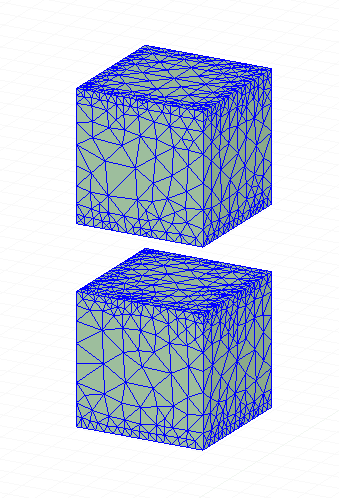
\includegraphics[width=0.5\linewidth]{p4/p4FIG3}
%    \vspace{-4mm}\caption{The mesh generated by ANSYS Maxwell after 25 passes of automatic mesh refinement for the magnetic configuration shown in Figure \ref{fig:p4cubeMagnetsRepulsion}. This mesh uses approximately 58,000 tetrahedral elements with quadratic shape functions, with approximately 4,500 elements per magnet and 49,000 elements in the region between and around the magnets.}
%    \label{fig:p4cubeMesh}
%\end{figure}
\begin{figure}
    \centering
    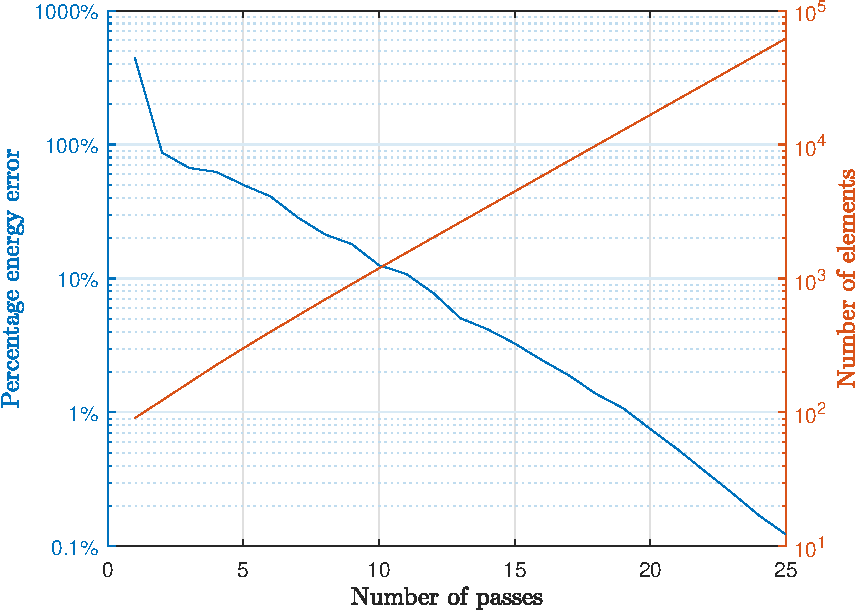
\includegraphics[width=0.8\textwidth]{p4/p4FIG4}
    \caption{Percentage energy error and number of tetrahedral elements in the ANSYS Maxwell simulation for \(d = 0.5\) as the number of passes of automatic mesh generation is increased.}
    \label{fig:p4repulseConvergence}
\end{figure}
\begin{figure}
	\centering
	\includegraphics[width=0.8\linewidth]{p4/p4FIG5}
	\caption{Nondimensionalised force between the two magnets in Figure \ref{fig:p4cubeMagnetsRepulsion} for \(\mu_r = 1\) (calculated using \cite{Akoun1984}), \(\mu_r = 1.05\), \(\mu_r = 1.2\), and \(\mu_r = 3\). The forces calculated using the methodology presented in this paper are denoted with lines, with finite element simulations represented with large dots. The methodology presented above is in strong agreement with the finite element simulations, indicating correct force results.}
	\label{fig:p4cubeMagnetForces}
\end{figure}

In this simple repulsion configuration, it can be seen in Figure \ref{fig:p4cubeMagnetForces} that modelling neodymium magnets with \(\mu_r = 1\) overestimates the force by at least 4\%. While this is a nontrivial error, it is often accurate enough for preliminary designs. However, more permeable magnetic materials may give considerably larger errors. For this configuration, modelling hard ferritic magnets and alnico magnets with \(\mu_r = 1\) overestimates the force by at least 17\% and 170\% respectively. Thus, consideration of relative permeability in magnetostatic analysis is of high importance in electromagnetic design.

\subsection{Rotated magnets}
To verify the calculation of torque, a similar example is presented. Two cuboidal magnets, shown in Figure \ref{fig:p4cubeMagnetsRotated}, are positioned with a distance of \(3l/2\) between their centres. Initially, both magnets are parallel and magnetised along the positive vertical direction. The bottom magnet is rotated about its centre, and the force and torque on the magnet evaluated as it is rotated. The forces are nondimensionalised using Equation (\ref{eqn:p4forceNormalisation}) and the torques nondimensionalised by
\begin{equation}
	\hat{T} = \frac{\mu_0}{l^3 B_{r\text{,top}} B_{r,\text{bot}}} T \text{.}
\end{equation}
In addition, finite element simulations were conducted to examine error in the solutions found using this methodology. After 25 passes, the finite element mesh was similar to that obtained in Section \ref{sec:p4verification:magnetsRepulsion}, using approximately 58,000 tetrahedral elements, with approximately 4,500 elements per magnet and 49,000 elements in the region between and around the magnets. The percentage energy error and number of tetrahedral elements for \(\theta =\ \)\ang{60} at each pass is shown in Figure \ref{fig:p4rotateConvergence}, indicating convergence in the simulations. The torque results are plotted in Figure \ref{fig:p4cubeMagnetRotatedTorquex}, with the force results in Figures \ref{fig:p4cubeMagnetRotatedForcey} and \ref{fig:p4cubeMagnetRotatedForcez}.
\begin{figure}
	\centering
	\begin{tikzpicture}

% Set up coordinates of vertices
\coordinate(toptl) at (-1,4);
\coordinate(toptr) at (1,4);
\coordinate(topbl) at (-1,2);
\coordinate(topbr) at (1,2);
\coordinate(bottl) at (0.366,1.366);
\coordinate(bottr) at (-1.366,0.366);
\coordinate(botbl) at (1.366,-0.366);
\coordinate(botbr) at (-0.366,-1.366);

% Draw magnets
\draw (toptl) -- (toptr) -- (topbr) -- (topbl) -- cycle;
\draw (bottl) -- (bottr) -- (botbr) -- (botbl) -- cycle;

% Draw magnetisation vectors
\draw[->,thick] (0,2.5) -- (0,3.5);
\draw[->,thick] (0.25,-0.433) -- (-0.25,0.433);
\node(Mtop) at (0.5,3) {\(\mathbf{B}_{r\text{,top}}\)};
\node(Mbot) at (0.55,-0) {\(\mathbf{B}_{r\text{,bot}}\)};

% Draw centres
%\node(ctop) at (0,4) {\textbf{.}};
%\node(cbot) at (0,0) {\textbf{.}};

% Draw dimensions
\draw[<->] (2,2) -- (2,4);
\node(lsidetop) at (1.8,3) {\(l\)};
\draw[<->] (-2.232,-0.134) -- (-1.232,-1.866);
\node(lsidebot) at (-1.99,-1.15) {\(l\)};
\draw[<->] (1.866,-1.232) -- (0.134,-2.232);
\node(lunder) at (0.9,-1.559) {\(l\)};
\draw[<->] (-3,0) -- (-3,3);
\node(d) at (-3.25,1.5) {\(\frac{3l}{2}\)};

% Draw horizontal centrelines
\draw[dashed,gray] (0,3) -- (-3,3);
\draw[dashed,gray] (0,0) -- (-3,0);

% Draw angle
\draw[dashed] (0,0) -- (0,1.5);
\draw[dashed] (0,0) -- (-0.75,1.3);
\node(theta) at (-0.175,0.65) {\(\theta\)};

\end{tikzpicture}
	\caption{Two cube magnets with a side length of \(l\) maintaining a constant distance of \(3l/2\) between their centres. The force and torque on the bottom magnet is calculated as it is rotated an angle \(\theta\) about its centre.}
	\label{fig:p4cubeMagnetsRotated}
\end{figure}
\begin{figure}
    \centering
    \includegraphics[width=0.8\linewidth]{p4/p4FIG7}
    \caption{Percentage energy error and number of tetrahedral elements in the ANSYS Maxwell simulation for \(\theta =\ \)\ang{60} as the number of passes of automatic mesh generation is increased.}
    \label{fig:p4rotateConvergence}
\end{figure}
\begin{figure}
	\centering
	\includegraphics[width=0.8\linewidth]{p4/p4FIG8}
	\caption{Nondimensional torque on the bottom magnet about the axis of rotation of the magnet as it rotates for varying relative permeabilities \(\mu_r\). Finite element results are depicted with large dots, indicating some agreement with the results using the above methodology, with the FEA results being approximately 2\% smaller in magnitude for low permeabilities.}
	\label{fig:p4cubeMagnetRotatedTorquex}
\end{figure}
\begin{figure}
	\centering
	\includegraphics[width=0.8\linewidth]{p4/p4FIG9}
	\caption{Nondimensional horizontal force \(F_H\) on the bottom magnet as it rotates for varying relative permeabilities \(\mu_r\). Finite element results are depicted using large dots, indicating strong agreement with the results using the above methodology.}
	\label{fig:p4cubeMagnetRotatedForcey}
\end{figure}
\begin{figure}
	\centering
	\includegraphics[width=0.8\linewidth]{p4/p4FIG10}
	\caption{Nondimensional vertical force \(F_V\) on the bottom magnet as it rotates for varying relative permeabilities \(\mu_r\). Finite element results are depicted using large dots, indicating strong agreement with the results using the above methodology.}
	\label{fig:p4cubeMagnetRotatedForcez}
\end{figure}
Figures \ref{fig:p4cubeMagnetRotatedTorquex}, \ref{fig:p4cubeMagnetRotatedForcey}, and \ref{fig:p4cubeMagnetRotatedForcez} show that the results obtained match closely with the finite element data. A small error between the estimated and FEA force results can be seen, with a larger error between the estimated and FEA torque results. To determine the source of this error, a special case of this configuration was used by setting \(\theta =\ \)\ang{90} and \(\mu_r = 1\). Since the magnets have parallel faces and a relative permeability of unity in this particular case, equations published by \textcite{Akoun1984} and \textcite{Janssen2010} can be used to calculate the exact force and torque respectively. The exact force in the horizontal direction and torque about the axis of rotation were calculated and compared to the results obtained using the methodology in this paper and finite element results, and are shown in Table \ref{tab:p4analyticTorque}.
\begin{table*}
    \centering
    \begin{tabular}{l|cc|cc}
    Method & $\hat F_H$ & Error & $\hat T$ & Error \\
    \hline
    Exact [4], [8] & $-0.04127$ & --- & $-0.04200$ & --- \\
    This work & $-0.04126$ & $0.02\%$ & $-0.04201$ & $0.24\%$ \\
    FEA & $-0.04120$ & $0.17\%$ & $-0.04107$ & $2.20\%$ \\
    \end{tabular}
    \caption{Nondimensional horizontal force \(\hat{F}_H\) and torque about the axis out of the page \(\hat{T}\) on the bottom magnet in Figure \ref{fig:p4cubeMagnetsRotated} at an angle of \ang{90} with both magnets having a relative permeability of \(\mu_r = 1\). The work presented here uses approximately 6,000 triangular surface elements, whereas the finite element simulations use approximately 58,000 tetrahedral volume elements. The work presented here has a considerably smaller percentage error than the finite element results when compared to the exact analytic results \cite{Akoun1984,Janssen2010}, indicating high accuracy of the work presented in this paper.}
    \label{tab:p4analyticTorque}
\end{table*}
It can be seen that for both force and torque, the results obtained using this methodology are considerably more accurate than the finite element results, with a percentage error almost ten times smaller. It appears that the finite element results are underestimating the force and torque, which may explain the discrepancy in Figures \ref{fig:p4cubeMagnetRotatedTorquex}, \ref{fig:p4cubeMagnetRotatedForcey}, and \ref{fig:p4cubeMagnetRotatedForcez}.

Interestingly, Figures \ref{fig:p4cubeMagnetRotatedTorquex}, \ref{fig:p4cubeMagnetRotatedForcey}, and \ref{fig:p4cubeMagnetRotatedForcez} show asymmetry when \(\mu_r \neq 1\). This is particularly visible in Figure \ref{fig:p4cubeMagnetRotatedTorquex} when \(\mu_r = 3\) between \(\theta =\ \)\ang{60} and \(\theta =\ \)\ang{120}, but this asymmetry occurs in all three plots and becomes more apparent as \(\mu_r\) is increased. This asymmetry is a result of the magnets producing fields which either strengthen or weaken the magnetisation of the other. When \(\theta <\ \)\ang{90}, the vertical component of the net field produced by the bottom magnet on the surface of the top magnet is in the same direction as \(\mathbf{B}_{r\text{,top}}\), thus strengthening the magnetisation of the top magnet. In the same way, the top magnet produces a field which strengthens the magnetisation of the bottom magnet. However, when \(\theta >\ \)\ang{90}, the opposite is true: Each magnet produces a field which weakens the magnetisation of the other magnet. Thus, each magnet strengthens the magnetisation of the other for \(\theta <\ \)\ang{90} and weakens the magnetisation of the other for \(\theta >\ \)\ang{90}, resulting in an asymmetry across \(\theta =\ \)\ang{90}, with a smaller magnitude of force and torque on the right side of each plot and a larger magnitude on the left.

In addition to verifying the force and torque, the magnetic field calculation is verified using the magnetic configuration in Figure \ref{fig:p4cubeMagnetsRotated} with \(\theta =\ \)\ang{90} and \(\mu_r = 3\) (as seen in Figure \ref{fig:p4cubeMagnetRotatedImage}). The magnetic field strength was calculated on the plane between the two magnets using the methodology in Section \ref{sec:p4magneticField} and nondimensionalised by the remanence magnetisation \(B_r\). In addition, finite element simulations were conducted on the same system using ANSYS Maxwell. The magnetic field strength computed using Section \ref{sec:p4magneticField} is plotted in Figure \ref{fig:p4cubeMagnetRotatedField}, along with the magnetic field strength generated by finite element simulations. The error is negligible, with a maximum error of 0.3\% of the remanence magnetisation, indicating the methodology used is calculating magnetic fields accurately.
\begin{figure}
	\centering
	\includegraphics[width=0.55\linewidth]{p4/p4FIG11}
	\caption{The surface charge densities of the magnets in Figure \ref{fig:p4cubeMagnetsRotated} when \(\theta =\ \)\ang{90} and \(\mu_r = 3\). Due to the relatively large permeability, the top surface of the bottom magnet has considerably more positive surface charges accumulating than negative charges.}
	\label{fig:p4cubeMagnetRotatedImage}
\end{figure}
\begin{figure}
	\centering
	\includegraphics[width=0.5\linewidth]{p4/p4FIG12}
	\caption{The magnetic field strength \(\left| \mathbf{B} \right|\) normalised by \(B_r\) on the plane between the two magnets in Figure \ref{fig:p4cubeMagnetsRotated} when \(\theta =\ \)\ang{90}. The projections of the magnets onto the plane are displayed using white dashed lines. The field was calculated using the methodology in this paper (top) and finite element simulations (middle), with the absolute error between the two calculated (bottom). This shows strong agreement, with a maximum error of 0.3\% of the remanence magnetisation.}
	\label{fig:p4cubeMagnetRotatedField}
\end{figure}
\section{Computational performance}\label{sec:p4computationalPerformance}
In contrast to other methods, this methodology has been designed in such a way that the magnetic field \(\mathbf{B}\) needs to be calculated only once, but requires the inversion of a potentially large non-sparse matrix (performed using the backslash operator or \texttt{mldivide} function in MATLAB). As such, it is considerably faster than the iterative methods often seen in literature, but requires more computational memory. In addition, this method uses an analytical equation \cite{OConnell2020a} to calculate the magnetic field, making it faster than finite element methods to obtain an accurate solution.

\subsection{Computational speed}
To assess computation speed, a simple magnetic system was defined using two cube magnets in repulsion, separated by one magnet width, equivalent to Figure \ref{fig:p4cubeMagnetsRepulsion} with \(d = l\). To assess accuracy, the relative permeability of the magnets was set to unity, \(\mu_r = 1\), which allows the use of exact analytic force equations published by \textcite{Akoun1984}. The force was calculated using both the methodology defined in this paper, finite element simulations, and the exact force equations using MATLAB R2020a on a personal computer with an Intel Xeon E3-1240 v5 at 3.50GHz with 16GB of memory. The force calculations using finite element simulations and the methodology in this paper were repeated with varying mesh densities and timed to give an indication of computation speed. Both methods were compared to the exact analytic force equations \cite{Akoun1984} to give a measure of error, with both methods showing approximately the same rate of error convergence, but with the methodology in this paper giving results approximately an order of magnitude faster for the same accuracy. The percentage error between the estimated force using the method in this paper and exact force was computed and is displayed in Figure \ref{fig:p4calculationTime}.
\begin{figure}
	\centering
	\includegraphics[width=0.8\linewidth]{p4/p4FIG13}
	\caption{Percentage error in the calculation of vertical force \(F_V\) between the magnets shown in Figure \ref{fig:p4cubeMagnetsRepulsion} with \(d = l\) and \(\mu_r = 1\) as mesh density, and thus calculation time, is increased. The number of surface mesh elements \(N\) is also plotted, showing an inverse trend when compared to the percentage error.}
	\label{fig:p4calculationTime}
\end{figure}

As expected, the percentage error decreases as calculation time increases. For this particular magnetic configuration and computation hardware, finite element simulations generally took more than 5s to achieve an error within 1\%. In contrast, the methodology in this paper took less than 100ms to attain less than 1\% error and less than 5s to attain less than 0.1\% error. This will vary depending on magnetic configuration, code implementation, and computation hardware, but gives an indication of the expected order of magnitude of calculation time to achieve a desired accuracy.

\subsection{Memory requirements}
This methodology requires more computational memory than other methods found in literature. Iterative methods, for example, require enough memory to keep track of the surface charge densities, but must recalculate the magnetic field information at each step. This can be done using a single \(N\times 1\) vector. In contrast, this method requires storing several large \(N\times N\) matrices of floating point numbers, as well as enough memory to invert a large \(\left(N+M\right) \times \left(N+M\right)\) matrix. This is a significantly larger memory requirement than iterative methods, but results in a considerably faster solution. During testing by the authors, a high precision calculation may use more than one gigabyte of memory, with equivalent finite element simulations requiring tens of gigabytes of memory. While considerable memory requirements are necessary for the method outlined in this paper, mesh optimisation was not considered. As such, testing was done using a basic mesh, with all elements being similar in size. If a more appropriate mesh is chosen, with finer mesh in areas with large magnetic field gradient, a high precision calculation can be done using less memory.

\subsection{Meshing considerations}
In this paper, a surface mesh has been used under the assumption that the magnetic permeability and remanence magnetisation vector are constant and uniform. If these assumptions are not valid, a volume mesh may be used and a similar methodology applied, where the magnetisation vector of each volume element is computed rather than the scalar surface charge density. However, the use of a volume mesh rather than surface mesh comes with a more considerable computation cost. Solving for the magnetisation vector field requires solving a large linear equation for each of the three Cartesian directions, while the scalar surface charge density solution only requires a single linear equation. In addition, calculation of the field produced by each element would require either using an inaccurate point dipole model, or calculating the field contribution from each of the surfaces of the element \cite{OConnell2020,OConnell2020a}. The use of the point dipole model considerably decreases accuracy for nearby elements, and the more complicated method considerably increases calculation time. These factors lead to a significantly larger computation cost when applying a volume mesh and solving the magnetisation vector field. Thus, for systems with constant and uniform permeability and remanence magnetisation, a surface charge density approach is preferred.

The methodology in this work uses a triangular surface mesh generated by finding the minimum convex hull of a set of vertices using the Geom3D library in the MatGeom package in MATLAB \cite{Legland2021}. Subdivision of the surface mesh is performed by dividing each triangular element into four congruent triangles until a desired number of surface elements was achieved. A triangular surface mesh has been chosen since analytic field equations are available for these elements \cite{OConnell2020a,OConnell2020}. These equations may be used to solve for the field produced by a triangle with constant surface charge density, and are highly efficient, especially when many field calculations are performed. In addition, a triangular surface mesh can represent any polyhedral surface and can be used to approximate curved surfaces, enabling the approximate solution of any magnetic configuration. The meshing algorithm itself is out of the scope of this work, since it is focused only on calculating the charge densities on each surface element and the resulting fields, forces, and torques. However, alternative meshing algorithms may be applied, and future analysis could be done on optimising the meshing process for this methodology.

\section{Conclusion}\label{sec:p4conclusion}
This paper has outlined a new algorithm for modelling magnetic materials with nonunity relative permeability. Assuming constant uniform magnetisation and constant permeability, the algorithm uses a one-step matrix inversion to solve for the surface charge density, magnetic field, force, and torque. In contrast to other methods available in literature, this method calculates magnetic field information only once, leading to a considerable increase in calculation speed. In addition, using a triangular surface mesh gives this methodology high versatility, allowing the modelling of any polyhedral magnet, and approximate modelling of any general magnet geometry.

The algorithm was verified against literature and finite element simulations using several magnetic configurations. A simple magnetic configuration was defined with two cube magnets in repulsion with varying permeabilities, with the force between the magnets calculated. The force results showed strong agreement with finite element simulations. In addition, it was shown that the permeability has a significant effect on the force between the magnets, and as such, care must be taken when assuming a relative permeability of unity. A similar magnetic configuration was used to verify the torque, where the magnets maintain a constant distance between their centres, but one magnet is rotated. The torque results were in agreement with finite element simulations, and it was again shown that permeability greatly affects torque. Furthermore, the magnetic field was calculated on the plane between the magnet centres with \(\theta =\ \)\ang{90}. Finite element simulations showed strong agreement, with a negligible error.

This methodology has allowed fast and accurate results for any magnet geometry and configuration. This can be used for fast optimisation of electromagnetic designs, giving more accurate results than analytic methods which assume unity relative permeability, and faster results than finite element simulations.
\begin{subappendices}
\addcontentsline{toc}{section}{\protect\numberline{}Appendices}
\addtocontents{toc}{\protect\setcounter{tocdepth}{-1}}
\renewcommand{\thesection}{Appendix \arabic{chapter}.\Alph{section}}
\section{Volume charge density}\label{sec:p4noVolumeCharge}
Consider a magnetic material with constant permeability \(\mu_r\) and constant uniform remanence magnetisation \(\mathbf{B}_r\). According to Equation (\ref{eqn:p4equivalentMagnetisation}), this material will satisfy the equation
\begin{equation}
    \mathbf{M} = \frac{\mu_r - 1}{\mu} \mathbf{B} + \frac{1}{\mu} \mathbf{B}_r \text{.}
\end{equation}
To calculate the volume charge density \(\nabla \cdot \mathbf{M}\), take the divergence of both sides, giving
\begin{equation}
    \nabla \cdot \mathbf{M} = \nabla \cdot \left( \frac{\mu_r - 1}{\mu} \mathbf{B} \right) + \nabla \cdot \left( \frac{1}{\mu} \mathbf{B}_r \right) \text{.}
\end{equation}
However, under the assumption of constant permeability, the permeability terms can be taken out of the divergence,
\begin{equation}\label{eqn:p4divM}
    \nabla \cdot \mathbf{M} = \frac{\mu_r - 1}{\mu} \nabla \cdot \mathbf{B} + \frac{1}{\mu} \nabla \cdot \mathbf{B}_r \text{.}
\end{equation}
Maxwell's equations state that the \(\mathbf{B}\) field is solenoidal, \(\nabla \cdot \mathbf{B} = 0\). In addition, the assumption of constant uniform remanence magnetisation leads to \(\nabla \cdot \mathbf{B}_r = 0\). Consequently, the right side of Equation (\ref{eqn:p4divM}) becomes zero, and therefore
\begin{equation}
    \nabla \cdot \mathbf{M} = 0 \text{.}
\end{equation}
Thus, a material with constant uniform remanence magnetisation and constant permeability has no volume charge density and the volume integral for the charge method may be neglected.
\section{Matrix invertibility}\label{sec:p4invertibleMatrix}
Consider the system defined by the matrix equation
\begin{equation}\label{eqn:p4invertibleProofEquation}
    C \bm{\sigma} = K \bm{\sigma}_0 \text{,}
\end{equation}
where \(C\) is an \(N\times N\) square matrix and \(\bm{\sigma}\) and \(\bm{\sigma}_0\) are \(N\times 1\) vectors of final and initial surface charge densities respectively. This section will show that the matrix \(C\) is invertible using contradiction.

Suppose \(C\) has at least one eigenvalue equal to zero, \(\lambda = 0\). This implies that there exists a \textit{non-zero} eigenvector \(\bm{\sigma}\) of \(C\) such that
\begin{equation}
    C\bm{\sigma} = \lambda \bm{\sigma} = 0 \bm{\sigma} = \mathbf{0} \text{.}
\end{equation}
Substituting this into Equation (\ref{eqn:p4invertibleProofEquation}) leads to
\begin{equation}
    K \bm{\sigma}_0 = \mathbf{0} \text{.}
\end{equation}
Since \(\mu_r\) is a finite positive value for the magnetic materials considered in this work, \(K \neq 0\), and thus,
\begin{equation}
    \bm{\sigma}_0 = \mathbf{0} \text{.}
\end{equation}
We know that \(\bm{\sigma} \neq \mathbf{0}\) by the definition of an eigenvector. Thus, this implies that there exists a system with zero initial magnetic charge density, \(\bm{\sigma}_0 = \mathbf{0}\), which becomes spontaneously magnetised, such that \(\bm{\sigma} \neq \mathbf{0}\), with no external field. This is clearly absurd, and the assumption of any eigenvalues being equal to zero fails. Thus, all eigenvalues of \(C\) must be nonzero and therefore \(C\) must be invertible.

While \(C\) is invertible, it may have an undesirable condition number, leading to errors when inverting. However, this method uses constrained least squares, and \(C\) is never directly inverted; it is simply shown here to be invertible to imply a solution for \(\bm{\sigma}\) exists.
\section{Surface charge density over a magnet}\label{sec:p4integralSigma}
Taking the divergence of Equation (\ref{eqn:p4equivalentMagnetisation}) inside the volume \(V\) of a magnetic body gives
\begin{equation}
    \nabla \cdot \mathbf{M} = \nabla \cdot \left( \frac{\mu_r-1}{\mu} \mathbf{B} \right) + \nabla \cdot \left( \frac{1}{\mu} \mathbf{B}_r \right) \text{.}
\end{equation}
Assuming the permeability \(\mu\) is constant (and thus \(\mu_r\) is also constant), the permeability terms may be taken out of the divergence operators,
\begin{equation}
    \nabla \cdot \mathbf{M} = \frac{\mu_r-1}{\mu} \nabla \cdot \mathbf{B} + \frac{1}{\mu} \nabla \cdot \mathbf{B}_r \text{.}
\end{equation}
However, we know that \(\mathbf{B}\) is divergence-free from Maxwell's equations. In addition, we are assuming that the remanence magnetisation inside the volume \(V\) is constant and uniform, implying it is also divergence-free. Therefore, inside the volume of a magnet, \(\nabla \cdot \mathbf{B} = 0\) and \(\nabla \cdot \mathbf{B}_r = 0\), and
\begin{equation}
    \nabla \cdot \mathbf{M} = 0 \text{.}
\end{equation}
We can then take the volume integral of this expression inside the volume \(V\), giving
\begin{equation}
    \iiint_V \nabla \cdot \mathbf{M}\ dv = 0 \text{.}
\end{equation}
Finally, since \(\mathbf{M}\) is assumed to be well-behaved inside the magnet, we can apply the divergence theorem to the integral, giving
\begin{equation}
    \oiint_S \mathbf{M} \cdot \hat{\mathbf{n}}\ ds = 0 \text{.}
\end{equation}
Since the surface charge density is given by \(\sigma = \mathbf{M} \cdot \hat{\mathbf{n}}\), we finally obtain
\begin{equation}\label{eqn:p4integralSigma}
    \oiint_S \sigma \ ds = 0 \text{.}
\end{equation}
\end{subappendices}
\clearpage
\section*{Author's remarks on Chapter \ref{chap:paper4}}
This chapter presents the final article submitted in this thesis, and successfully modelled permanent magnets with non-unity relative permeability using a semi-analytic approach. While this method is fast and highly accurate, it does require the assumption of constant permeability, and is unable to accurately model non-linear magnetic materials. However, permanent magnets are generally highly linear in their operating regions, and as such this method models them accurately. While the approaches seen in Chapters \ref{chap:paper1} and \ref{chap:paper2} are considerably faster to evaluate than this method, they cannot model non-unity relative permeability and will see several percentage points of error when modelling real permanent magnets. This method is slower, but far more accurate, and when combined with the field equations from Chapter \ref{chap:paper2}, can accurately model any permanent magnet of any shape.
\addtocontents{toc}{\protect\setcounter{tocdepth}{2}}

\newpage
\section*{References}
\addcontentsline{toc}{section}{\protect\numberline{}References}
\printbibliography[heading=none]
\chapter{Thesis summary}\label{chap:conclusion}
\fancyhead[LE]{\scshape Chapter\ \ref{chap:conclusion}}

Geometry-based analytic modelling of the magnetostatic fields began in the late twentieth century, and despite decades of research, limitations in current models are present to this day. This thesis attempts to address some of these limitations, with a particular focus on the geometry and permeability of a permanent magnet. Throughout this project, several milestones were achieved, but there is still more scope for future projects on the modelling of permanent magnets. This chapter concludes this thesis by summarising the work completed to date and outlining potential future work following this research.

\section{Primary research outcomes}
The overarching outcome of this thesis is the development of accurate and fast methodologies for the modelling of permanent magnets, and is summarised in this section.

\subsection{Magnetic field equations for ideal polyhedral magnets}
The first major outcome of this project was the development of the magnetic field equations seen in Chapters \ref{chap:paper1} and \ref{chap:paper2}. These equations describe the magnetic field produced by any permanent magnet with polyhedral geometry, constant magnetisation, and a relative permeability of unity. These equations are derived with emphasis on computational efficiency, with each methodology having its own advantages and disadvantages. The first methodology (Chapter \ref{chap:paper1}) is most effective when the field is to be calculated at few points in space, such as when computing the electromagnetic force on a moving charged particle. In contrast, the second methodology (Chapter \ref{chap:paper2}) is most effective when calculating the field at many points, such as when finding the magnetostatic force between several permanent magnets. The equations present in both methodologies are readily programmable in any language on a personal computer. They consist only of logarithmic, trigonometric, and square root terms, and are thus highly computationally efficient, with no special functions or numeric integrals required to evaluate the magnetic field.

Due to their fast computation speed, these equations may be used for parametric optimisation studies where geometry or topology is varied. This can be used on large arrays of magnets while varying the geometry of each magnet to achieve a desired field pattern, such as that shown in Chapter \ref{chap:paper3}. In addition, the computation speed of the field equations allows multiple parameters to be simultaneously varied, such as geometry, magnet arrangement, and magnetisation state.

Furthermore, this methodology may be applied to any magnet composed of flat faces. A magnet with curved faces may be approximated with a polyhedral geometry, and this methodology applied, giving a highly accurate solution to the field produced by any permanent magnet geometry.

\subsection{Modelling magnetic permeability in polyhedral permanent magnets}
While it was shown in Chapters \ref{chap:paper1} and \ref{chap:paper2} that the magnetic field produced by a polyhedral magnet may be quickly evaluated, these methodologies do not consider non-unity relative permeability. Permanent magnets generally have relative permeabilities close to unity, but are usually between 1.05 and 1.15, leading to a modelling error when evaluating these fields, especially in the presence of other field sources. The second major outcome of this thesis was the development of a methodology to model magnetic materials with non-unity but constant relative permeability, described in Chapter \ref{chap:paper4}. Again, this methodology was developed with emphasis on computational efficiency, and attempts to circumvent the drawbacks associated with the methodologies found in literature. While most methods currently available are based on an iterative approach, requiring recalculating the magnetic field several times, this new method involves only a single field evaluation combined with a matrix inversion to solve the system in a single step. This method, in conjunction with the field calculation methodology from Chapter \ref{chap:paper2}, creates a highly effective and fast solution for the magnetic field produced by permeable polyhedral permanent magnets.

This methodology is based on the field calculation technique detailed in Chapter \ref{chap:paper2}, and thus may be applied to any magnet geometry. If magnets in a system have non-polyhedral geometry, they may be approximated with a polyhedral shape, allowing fast and accurate estimation of the fields produced by any permanent magnet geometry with constant non-unity relative permeability.

\subsection{Forces and torques between permeable polyhedral magnets}
Although the magnetic fields produced by polyhedral magnets are of interest, one of the most prominent applications of permanent magnets is in electromechanical actuators, where knowledge of the forces and torques is crucial. Thus, the final outcome of this thesis is the development of an accurate force and torque evaluation methodology for polyhedral magnets. This methodology may be applied to any polyhedral magnet geometry with constant non-unity permeability, as described in Chapter \ref{chap:paper4}, giving fast and highly accurate solutions for these parameters. In addition, non-polyhedral geometries may be approximated, allowing the use of this methodology. This outcome was shown to be significantly faster and more accurate than the industry standard finite element analysis in Chapter \ref{chap:paper4} with the assumptions of constant remanence magnetisation and permeability. This methodology may also be applied in a system with other magnetic field sources, as shown in Section \ref{sec:p4externalFields}, enabling fast and accurate computations of the fields, forces, and torques of any system composed of permanent magnets and external field sources.

\section{Future work}
Though this thesis has outlined methodologies to model permanent magnets of arbitrary geometry and non-unity constant relative permeability, there are still several open questions in this area. This section will outline current gaps in knowledge manifested as potential future work following this thesis.

\subsection{Analytic force and torque}
While the magnetic field equations were found analytically in this thesis by solving a double integral across triangular and trapezial surfaces, the forces and torques were evaluated numerically. In general, the forces and torques may be described by the magnetic charge model, which requires a further double or triple integral of the magnetic field expressions over a polygonal surface or polyhedral volume. Due to the rotation matrices involved, and the highly complicated expressions, these force and torque integrals are extremely difficult to solve analytically. Further work in this area would suggest attempting to find a solution to these integrals based on the field equations presented in this thesis. This would likely be performed again using triangular or trapezial surfaces, but due to the general rotations involved with these systems, these integrals may not have a solution. In this case, the suggested future work would consist of finding accurate approximations to the field distribution functions which are analytically integrable. This may consist of Taylor series representations, Fourier series approximations, or other field estimations. Since magnetic fields are generally well-behaved, with the \(\mathbf{B}\)-field being divergence-free, an accurate estimation in terms of integrable functions is likely attainable. Upon solving these approximate integrals, a set of force and torque equations may be produced, which would be extremely quick to evaluate and highly accurate. However, due to the nature of permeability, it is likely these equations would only be valid for magnetic materials with a relative permeability of unity.

\subsection{Non-linear permeability}
In Chapter \ref{chap:paper4}, a framework was defined in which the magnetic fields, forces, and torques may be evaluated quickly and accurately. However, this assumes a constant permeability in each magnetic material. Future work in this area would be based on deriving similar methodologies but generalising further to include non-linear permeability.

This methodology would likely require a volume mesh rather than a surface mesh, since under non-linear permeability, the assumption that \(\nabla \cdot \mathbf{M} = 0\) is not generally true. If a fine enough volume mesh is applied to a magnetic specimen such that the magnetisation vector field across each volume element is approximately constant, then \(\nabla \cdot \mathbf{M} \approx 0\) inside each element. Thus, the volume integral of the magnetic charge model may be neglected, and only the integrals across the surfaces of each volume element remain. The field equations from Chapters \ref{chap:paper1} or \ref{chap:paper2} could be used to calculate the field from each volume element on each other element, and the total field at each evaluated. Based on the field, the magnetisation vector of each element may be estimated based on the \(BH\) curve of the material. This process may be repeated until the magnetisation vectors converge, allowing the computation of the fields, forces, and torques.

While this methodology is not iteration-free, it allows evaluation of the magnetic fields due to non-linear permeability. In addition, the forces and torques may be easily calculated once the magnetisation vectors converge, similar to the methods found in Chapter \ref{chap:paper4}.

\subsection{Magnetic geometry and topology optimisation framework}
As seen in Chapter \ref{chap:paper3}, the speed of field calculations presented in this thesis allows fast parametric optimisation studies. This may be extended to include the effect of permeability, since magnets in an array often have a strong demagnetising effect on one another. Future work could involve developing a generalised framework for optimisation of magnetic systems, allowing variation of magnet geometry, magnetisation strength, and magnetisation direction. For example, to reduce force ripple in an iron-less electric motor, a particular field pattern based on the coil geometry is desired. An optimisation framework based on the methods found in this thesis could be defined, with magnet sizes and magnetisation strengths varied until a desired field pattern is achieved. Due to the emphasis on computational efficiency of the methods presented in this thesis, optimisation routines could be completed quickly, even under the effects of permeability, allowing fast optimisation of many magnetic systems.

\section{Concluding remarks}
This thesis has presented a set of algorithms that allow evaluation of magnetic fields, forces, and torques due to general permeable polyhedral permanent magnets with emphasis placed on computation speed. This emphasis permits fast optimisation of magnetic systems, allowing variations in magnet geometry, topology, and magnetisation. These methodologies represent a considerable contribution to the field of computational magnetostatics and magnetic modelling, with a focus on generalising and relaxing the strong geometry and permeability constraints currently found in literature. The author hopes that this inspires further research into generalised magnetic modelling and assists designers in further optimising their electromagnetic designs, leading to a future which is as attractive as a magnet on iron.
\appendix
\addcontentsline{toc}{chapter}{\protect\numberline{}Appendices}
\addtocontents{toc}{\protect\setcounter{tocdepth}{1}}
%\renewcommand{\thesection}{Appendix \arabic{chapter}.\Alph{section}}
\titleformat{\chapter}[display]{\normalfont\Huge\scshape}{Appendix \thechapter}{1em}{}
\chapter{Derivation of the magnetic charge model}\label{app:chargeModelDerivation}
\fancyhead[LE]{\scshape Appendix\ \ref{app:chargeModelDerivation}}
To prove the magnetic charge model, two main steps are performed. First, Helmholtz decomposition is proven for the magnetisation vector field \(\mathbf{M}\). Once this is done, the magnetic constitutive relation, \(\mathbf{B} = \mu_0 \left(\mathbf{H} + \mathbf{M}\right)\), is used to find expressions for the magnetic flux density \(\mathbf{B}\) and the magnetic field intensity \(\mathbf{H}\).

\section*{Helmholtz decomposition}
We begin with a volume \(V'\) of magnetic material bounded by a surface \(S'\). The magnetisation vector field \(\mathbf{M}\left(\mathbf{x}\right)\) is finite-valued inside \(V'\) and can therefore be written as a volume integral over the volume,
\begin{equation}\label{eqn:MintegralFormulation}
    \mathbf{M}\left(\mathbf{x}\right) = \iiint_{V'} \mathbf{M}\left(\mathbf{x}'\right) \delta^3 \left(\mathbf{x}-\mathbf{x}'\right)\ d^3v' \text{,}
\end{equation}
where \(\delta^3\left(\mathbf{x}-\mathbf{x}'\right)\) is the three-dimensional delta function. Usually, we constrain \(\mathbf{x}\) to be inside \(V'\), that is, \(\mathbf{x} \in V'\), since the integral is zero-valued if \(\mathbf{x} \notin V'\). However, the magnetisation vector field \(\mathbf{M}\left(\mathbf{x}\right)\) is also zero-valued everywhere outside the volume \(V'\). Thus, Equation (\ref{eqn:MintegralFormulation}) is valid for all \(\mathbf{x} \in \mathbb{R}^3\).

It is also known that the delta function \(\delta^3\) is given by the Laplacian of a Green's function,
\begin{equation}\label{eqn:laplacianGreens}
    \delta^3\left(\mathbf{x}-\mathbf{x}'\right) = \nabla^2 G\left(\mathbf{x},\mathbf{x}'\right) = \nabla'^2 G\left(\mathbf{x},\mathbf{x}'\right) \text{,}
\end{equation}
where
\begin{equation}\label{eqn:greensFunction}
    G\left(\mathbf{x},\mathbf{x}'\right) = -\frac{1}{4\pi\left| \mathbf{x}-\mathbf{x}' \right|}
\end{equation}
and \(\nabla'\) is the Laplacian with respect to the primed coordinates \(\mathbf{x}'\).

Equation (\ref{eqn:laplacianGreens}) can be applied to the integral in Equation (\ref{eqn:MintegralFormulation}), giving
\begin{equation}
    \mathbf{M}\left(\mathbf{x}\right) = \iiint_{V'} \mathbf{M}'\ \nabla^2 G\ d^3v' \text{,}
\end{equation}
where \(\mathbf{M}' = \mathbf{M}\left(\mathbf{x}'\right)\) and the arguments of the Green's function have been omitted for brevity.

Assuming \(\mathbf{M}\) is twice continuously differentiable inside the volume \(V'\), the identity
\begin{equation}\label{eqn:laplacianIdentity}
    \nabla^2 \left(G\mathbf{M}'\right) = \mathbf{M}'\ \nabla^2 G + 2\left(\nabla G \cdot \nabla\right)\mathbf{M}' + G \nabla^2 \mathbf{M}'
\end{equation}
is true. However, since \(\mathbf{M}'\) varies only with the primed coordinates, the Jacobian and Laplacian terms in Equation (\ref{eqn:laplacianIdentity}) become zero, leaving
\begin{equation}
    \nabla^2 \left(G\mathbf{M}'\right) = \mathbf{M}'\ \nabla^2G \text{.}
\end{equation}
Therefore,
\begin{equation}
    \mathbf{M}\left(\mathbf{x}\right) = \iiint_{V'} \nabla^2 \left(\mathbf{M}' G\right)\ d^3v' \text{.}
\end{equation}
The integrand is vector-valued, and the vector Laplacian identity
\begin{equation}
    \nabla^2 \mathbf{A} = \nabla \left( \nabla \cdot \mathbf{A}\right) - \nabla \times \left( \nabla \times \mathbf{A} \right)
\end{equation}
can be applied, giving
\begin{align}
    \mathbf{M}\left(\mathbf{x}\right) = \iiint_{V'} & \nabla \left( \nabla \cdot \left(\mathbf{M}' G \right) \right)\ d^3v' \nonumber \\
    & - \iiint_{V'} \nabla \times \left( \nabla \times \left(\mathbf{M}' G\right) \right)\ d^3v' \text{.}
\end{align}
Here, the gradient and curl operate on the unprimed coordinates, so can be moved inside the integrals, giving
\begin{align}
    \mathbf{M}\left(\mathbf{x}\right) = \nabla \iiint_{V'} \nabla & \cdot \left(\mathbf{M}' G \right) \ d^3v' \nonumber \\
    & - \nabla \times \iiint_{V'} \nabla \times \left( \mathbf{M}' G\right)\ d^3v' \text{.}
\end{align}
The first integrand can be expanded using the vector calculus product rule,
\begin{equation}
    \nabla \cdot \left( \mathbf{M}' G\right) = G\ \nabla \cdot \mathbf{M}' + \mathbf{M}' \cdot \nabla G \text{.}
\end{equation}
However, \(\mathbf{M}'\) is constant with respect to the unprimed coordinates, and as such \(\nabla \cdot \mathbf{M}' = 0\), and
\begin{equation}
    \nabla \cdot \left( \mathbf{M}' G\right) = \mathbf{M}' \cdot \nabla G \text{.}
\end{equation}
A similar identity can be used on the second integrand, giving
\begin{equation}
    \nabla \times \left( \mathbf{M}' G\right) = \mathbf{M}' \times \nabla G \text{.}
\end{equation}
Therefore,
\begin{align}
    \mathbf{M}\left(\mathbf{x}\right) = \nabla \iiint_{V'} & \mathbf{M}' \cdot \nabla G \ d^3v' \nonumber \\
    & - \nabla \times \iiint_{V'} \mathbf{M}' \times \nabla G\ d^3v' \text{.}
\end{align}

For the Green's function defined in Equation (\ref{eqn:greensFunction}), the gradient coordinate system can be modified from the unprimed coordinates to the primed coordinates using the identity \(\nabla G = -\nabla' G\), leading to
\begin{align}
    \mathbf{M}\left(\mathbf{x}\right) = -\nabla \iiint_{V'} & \mathbf{M}' \cdot \nabla' G \ d^3v' \nonumber \\
    & + \nabla \times \iiint_{V'} \mathbf{M}' \times \nabla' G\ d^3v' \text{.}
\end{align}
By rearranging the vector product rule on the divergence of \(G\mathbf{M}'\) with respect to the primed coordinates, we obtain
\begin{equation}
    \mathbf{M}' \cdot \nabla' G = \nabla' \cdot \left(G\mathbf{M}'\right) - G \nabla' \cdot \mathbf{M}' \text{.}
\end{equation}
By applying a similar identity to the curl of \(G\mathbf{M}'\), we obtain
\begin{equation}
    \mathbf{M}' \times \nabla' G = -\nabla' \times \left( G\mathbf{M}' \right) + G\ \nabla' \times \mathbf{M}' \text{.}
\end{equation}
Substituting these identities into the expression for \(\mathbf{M}\left(\mathbf{x}\right)\) gives
\begin{align}\label{eqn:chargeModelM_fourIntegrals}
    \mathbf{M}\left(\mathbf{x}\right) = -\nabla \left( -\iiint_{V'} G\ \nabla' \cdot \mathbf{M}'\ d^3v' + \iiint_{V'} \nabla' \cdot \left(G\mathbf{M}'\right) d^3v' \right) \nonumber \\
    -\nabla \times \left( \iiint_{V'} G\ \nabla' \times \mathbf{M}' d^3v' - \iiint_{V'} \nabla' \times \left( G\mathbf{M}'\right) d^3v' \right) \text{.}
\end{align}

The divergence theorem states that for a well-behaved vector field \(\mathbf{F}\) in a volume \(V'\) bounded by a surface \(S'\) with outward-facing unit normal vector \(\hat{\mathbf{n}}'\),
\begin{equation}
    \iiint_{V'} \nabla' \cdot \mathbf{F}\ d^3v' = \oiint_{S'} \mathbf{F} \cdot \hat{\mathbf{n}}'\ d^2s' \text{.}
\end{equation}
In addition, a corollary of the divergence theorem states
\begin{equation}
    \iiint_{V'} \nabla' \times \mathbf{F}\ d^3v' = -\oiint_{S'} \mathbf{F} \times \hat{\mathbf{n}}'\ d^2s' \text{.}
\end{equation}
These can be applied to the second and fourth integral in Equation (\ref{eqn:chargeModelM_fourIntegrals}), giving
\begin{align}
    \mathbf{M}\left(\mathbf{x}\right) = -\nabla \left( -\iiint_{V'} G\ \nabla' \cdot \mathbf{M}'\ d^3v' + \oiint_{S'} G\mathbf{M}' \cdot \hat{\mathbf{n}}'\ d^2s' \right) \nonumber \\
    -\nabla \times \left( \iiint_{V'} G\ \nabla' \times \mathbf{M}' d^3v' + \oiint_{S'} G\mathbf{M}' \times \hat{\mathbf{n}}'\ d^2s' \right) \text{,}
\end{align}
with \(G\) defined as in Equation (\ref{eqn:greensFunction}).

At this point, the magnetisation vector field is given by the gradient of some integral added to the curl of another integral. We can define a scalar potential \(\varphi\) and vector potential \(\mathbf{A}\) to simplify the expression for \(\mathbf{M}\left(\mathbf{x}\right)\), with
\begin{equation}
    \varphi\left(\mathbf{x}\right) = \frac{1}{4\pi} \iiint_{V'} \frac{\nabla' \cdot \mathbf{M}'}{\left| \mathbf{x} - \mathbf{x}'\right|}\ d^3v' - \frac{1}{4\pi} \oiint_{S'} \frac{\mathbf{M}'\cdot \hat{\mathbf{n}}'}{\left| \mathbf{x} - \mathbf{x}'\right|}\ d^2s' \text{, and}
\end{equation}
\begin{equation}
    \mathbf{A}\left(\mathbf{x}\right) = \frac{1}{4\pi} \iiint_{V'} \frac{\nabla' \times \mathbf{M}'}{\left| \mathbf{x} - \mathbf{x}'\right|}\ d^3v' + \frac{1}{4\pi} \oiint_{S'} \frac{\mathbf{M}'\times \hat{\mathbf{n}}'}{\left| \mathbf{x} - \mathbf{x}'\right|}\ d^2s' \text{,}
\end{equation}
giving
\begin{equation}
    \mathbf{M}\left(\mathbf{x}\right) = -\nabla \varphi\left(\mathbf{x}\right) + \nabla \times \mathbf{A}\left(\mathbf{x}\right) \text{.}
\end{equation}

Now we can apply the magnetostatic Maxwell's equations to the magnetisation vector field. Starting with
\begin{equation}
    \mathbf{B} = \mu_0 \left( \mathbf{H} + \mathbf{M} \right) \implies \mathbf{M} = \frac{1}{\mu_0} \mathbf{B} - \mathbf{H} \text{.}
\end{equation}
Therefore,
\begin{equation}\label{eqn:BHandPhiA}
    \frac{1}{\mu_0} \mathbf{B} - \mathbf{H} =  -\nabla \varphi + \nabla \times \mathbf{A} \text{.}
\end{equation}

\section*{Solving for the magnetic flux density and magnetic field intensity}
Equation (\ref{eqn:BHandPhiA}) implies that some part of the \(\mathbf{B}\)-field and some part of the \(\mathbf{H}\)-field sum to give \(-\nabla \varphi\), with the remaining \(\mathbf{B}\) and \(\mathbf{H}\) summing to give \(\nabla \times \mathbf{A}\). This can be written using
\begin{equation}\label{eqn:gradPhi}
    -\nabla \varphi = p\frac{1}{\mu_0} \mathbf{B} - q\mathbf{H} \text{, and}
\end{equation}
\begin{equation}\label{eqn:curlA}
    \nabla \times \mathbf{A} = \left(1-p\right)\frac{1}{\mu_0}\mathbf{B} - \left(1-q\right) \mathbf{H} \text{.}
\end{equation}
Taking the curl of Equation (\ref{eqn:gradPhi}) gives
\begin{equation}
    \nabla \times \left(-\nabla \varphi\right) = p\frac{1}{\mu_0}\nabla \times \mathbf{B} - q\nabla \times \mathbf{H} \text{.}
\end{equation}
However, we are assuming that \(\nabla \times \mathbf{H} = \mathbf{0}\). Furthermore, the curl of a gradient is zero, so \(\nabla \times \left( -\nabla \varphi\right) = \mathbf{0}\). Thus,
\begin{equation}
    p\nabla \times \mathbf{B} = \mathbf{0} \text{.}
\end{equation}
In general, the curl of \(\mathbf{B}\) is nonzero, implying that \(p = 0\). Equation (\ref{eqn:curlA}) then simplifies to
\begin{equation}
    \nabla \times \mathbf{A} = \frac{1}{\mu_0}\mathbf{B} - \left(1-q\right)\mathbf{H} \text{.}
\end{equation}
Taking the divergence of this equation gives
\begin{equation}
    \nabla \cdot \left( \nabla \times \mathbf{A} \right) = \frac{1}{\mu_0}\nabla \cdot \mathbf{B} - \left(1-q\right)\nabla \cdot \mathbf{H} \text{.}
\end{equation}
However, according to Maxwell's equations, \(\nabla \cdot \mathbf{B} = 0\). Therefore,
\begin{equation}
    \nabla \cdot \left( \nabla \times \mathbf{A} \right) = \left(1-q\right)\nabla \cdot \mathbf{H} \text{.}
\end{equation}
In general, \(\nabla \cdot \mathbf{H} \neq 0\). Thus, \(q = 1\) since \(\nabla \cdot \left( \nabla \times \mathbf{A} \right) = 0\) for any vector field \(\mathbf{A}\). Therefore, \(\varphi\) and \(\mathbf{A}\) can be written
\begin{equation}
    \nabla \varphi = \mathbf{H} \text{, and}
\end{equation}
\begin{equation}
    \nabla \times \mathbf{A} = \frac{1}{\mu_0} \mathbf{B} \text{.}
\end{equation}

Thus, we have obtained an equation for the \(\mathbf{H}\)-field, which is described by
\begin{equation}
    \mathbf{H} = \nabla \varphi \text{.}
\end{equation}
Finally, upon simplification, we obtain the equation for the \(\mathbf{H}\)-field in the magnetic charge model,
\begin{equation}
    \mathbf{H} = \frac{1}{4\pi} \oiint_{S'} \left( \nabla' \cdot \mathbf{M}' \right) \frac{\mathbf{x}-\mathbf{x}'}{\left|\mathbf{x}-\mathbf{x}'\right|^3} ds' - \frac{1}{4\pi} \iiint_{V'} \left( \mathbf{M}' \times \hat{\mathbf{n}} \right) \frac{\mathbf{x}-\mathbf{x}'}{\left|\mathbf{x}-\mathbf{x}'\right|^3} dv' \text{.}
\end{equation}
In free space, the \(\mathbf{B}\) and \(\mathbf{H}\) fields are proportional, and thus
\begin{equation}
    \mathbf{B} = \frac{\mu_0}{4\pi} \oiint_{S'} \left( \nabla' \cdot \mathbf{M}' \right) \frac{\mathbf{x}-\mathbf{x}'}{\left|\mathbf{x}-\mathbf{x}'\right|^3} ds' - \frac{\mu_0}{4\pi} \iiint_{V'} \left( \mathbf{M}' \times \hat{\mathbf{n}} \right) \frac{\mathbf{x}-\mathbf{x}'}{\left|\mathbf{x}-\mathbf{x}'\right|^3} dv' \text{.}
\end{equation}
\chapter{Derivation of the magnetic field equations defined in Chapter~\ref{chap:paper2}}\label{app:fieldEquations}
\fancyhead[LE]{\scshape Appendix\ \ref{app:fieldEquations}}
The field equations derived in Chapter \ref{chap:paper2} took a great deal of effort and analysis to produce. This appendix details the derivation of these field equations.

\section{First component of the field equations}
To begin, we will solve the \(x-\)integral given by
\begin{align}
    B_x = \frac{\mu_0 \mathbf{M}\cdot\hat{\mathbf{n}}}{4\pi} \int_{x_1}^{x_2} \int_{m_1x'+c_1}^{m_2x'+c_2} \frac{x_r-x'}{\left(\left(x_r-x'\right)^2+\left(y_r-y'\right)^2+\left(z_r-z'\right)^2\right)^\frac{3}{2}}\ dy' dx' \text{.}
\end{align}
We first consider the inner integral \(I_{xy'}\),
\begin{align}
    I_{xy'} = \int_{m_1x'+c_1}^{m_2x'+c_2} \frac{x_r-x'}{\left(\left(x_r-x'\right)^2+\left(y_r-y'\right)^2+\left(z_r-z'\right)^2\right)^\frac{3}{2}}\ dy' \text{.}
\end{align}
The numerator is a constant with respect to \(y'\) and can be taken out of the integral,
\begin{align}\label{eqn:Ixydash}
    I_{xy'} = \left(x_r-x'\right)\int_{m_1x'+c_1}^{m_2x'+c_2} \frac{1}{\left(\left(x_r-x'\right)^2+\left(y_r-y'\right)^2+\left(z_r-z'\right)^2\right)^\frac{3}{2}}\ dy' \text{.}
\end{align}
We now perform the substitution given by
\begin{align}
    \tan\left(u\right) = \frac{y_r-y'}{\sqrt{\left(x_r-x'\right)^2+\left(z_r-z'\right)^2}} \text{.}
\end{align}
Rearranging this substitution yields
\begin{align}
    y' = y_r - \tan\left(u\right)\sqrt{\left(x_r-x'\right)^2+\left(z_r-z'\right)^2} \text{,}
\end{align}
which can be differentiated giving
\begin{align}\label{eqn:dydash}
    dy' = -\sec^2\left(u\right)\sqrt{\left(x_r-x'\right)^2+\left(z_r-z'\right)^2}\ du \text{.}
\end{align}
Here, the square root term behaves as a constant since \(x'\), \(y'\), and \(z'\) are mutually independent and we are integrating only with respect to \(y'\). Additionally, we can rearrange for the term \(\left(y_r-y'\right)^2\), giving
\begin{align}\label{eqn:yminusydashsquared}
    \left(y_r-y'\right)^2 = \left(\left(x_r-x'\right)^2+\left(z_r-z'\right)^2\right)\tan^2\left(u\right) \text{.}
\end{align}
We now substitute Equations (\ref{eqn:dydash}) and (\ref{eqn:yminusydashsquared}) into Equation (\ref{eqn:Ixydash}) and simplify, giving
\begin{align}
    I_{xy'} = \left(x_r-x'\right)\int_{y'=m_1x'+c_1}^{y'=m_2x'+c_2} \frac{-\sec^2\left(u\right)\sqrt{\left(x_r-x'\right)^2+\left(z_r-z'\right)^2}}{\left(\left(\left(x_r-x'\right)^2+\left(z_r-z'\right)^2\right)\left(1+\tan^2\left(u\right)\right)\right)^\frac{3}{2}}\ du \text{.}
\end{align}
Applying the trigonometric identity \(\sec^2\left(u\right) = 1+\tan^2\left(u\right)\) and further simplification gives
\begin{align}
    I_{xy'} &= \left(x_r-x'\right)\int_{y'=m_1x'+c_1}^{y'=m_2x'+c_2} \frac{-\sec^2\left(u\right)\sqrt{\left(x_r-x'\right)^2+\left(z_r-z'\right)^2}}{\sqrt{\left(x_r-x'\right)^2+\left(z_r-z'\right)^2}^3\left(\sec^2\left(u\right)\right)^\frac{3}{2}}\ du \\
    &= \left(x_r-x'\right)\int_{y'=m_1x'+c_1}^{y'=m_2x'+c_2} \frac{-\sec^2\left(u\right)}{\left(\left(x_r-x'\right)^2+\left(z_r-z'\right)^2\right)^2\sec^3\left(u\right)}\ du \\
    &= \left(x_r-x'\right)\int_{y'=m_1x'+c_1}^{y'=m_2x'+c_2} \frac{-\cos\left(u\right)}{\left(\left(x_r-x'\right)^2+\left(z_r-z'\right)^2\right)^2}\ du \text{.}
\end{align}
Since the square root term in Equation (\ref{eqn:dydash}) behaves as a constant, we can move the denominator outside the integral,
\begin{align}
    I_{xy'} &= -\frac{x_r-x'}{\left(\left(x_r-x'\right)^2+\left(z_r-z'\right)^2\right)^2}\int_{y'=m_1x'+c_1}^{y'=m_2x'+c_2} \cos\left(u\right)\ du \\
    &= -\frac{x_r-x'}{\left(\left(x_r-x'\right)^2+\left(z_r-z'\right)^2\right)^2} \Big[\sin\left(u\right)\Big]_{y'=m_1x'+c_1}^{y'=m_2x'+c_2} \text{.}
\end{align}
Now we will convert from \(u\) back to \(y'\). Based on the initial definition for \(u\), we can use basic trigonometry to obtain
\begin{align}
    \sin\left(u\right) = \frac{y_r-y'}{\sqrt{\left(x_r-x'\right)^2+\left(y_r-y'\right)^2+\left(z_r-z'\right)^2}} \text{.}
\end{align}
We can now substitute in the expression for \(\sin\left(u\right)\) and the limits for \(y'\), giving
\begin{align}
    I_{xy'} &= \frac{\left(x_r-x'\right)\left(y_r-m_1x'-c_1\right)}{\left(\left(x_r-x'\right)^2+\left(z_r-z'\right)^2\right)\sqrt{\left(x_r-x'\right)^2+\left(y_r-m_1x'-c_1\right)^2+\left(z_r-z'\right)^2}} \nonumber \\
    & -\frac{\left(x_r-x'\right)\left(y_r-m_2x'-c_2\right)}{\left(\left(x_r-x'\right)^2+\left(z_r-z'\right)^2\right)\sqrt{\left(x_r-x'\right)^2+\left(y_r-m_2x'-c_2\right)^2+\left(z_r-z'\right)^2}} \text{.}
\end{align}
With the first integral for the \(x\)-field solved, the expression now becomes
\begin{align}
    &B_x = -\frac{\mu_0\mathbf{M}\cdot\hat{\mathbf{n}}}{4\pi} \int_{x'=x_1}^{x'=x_2} \nonumber \\
    & - \frac{\left(x_r-x'\right)\left(y_r-m_1x'-c_1\right)}{\left(\left(x_r-x'\right)^2+\left(z_r-z'\right)^2\right)\sqrt{\left(x_r-x'\right)^2+\left(y_r-m_1x'-c_1\right)^2+\left(z_r-z'\right)^2}} \nonumber \\
    & \frac{\left(x_r-x'\right)\left(y_r-m_2x'-c_2\right)}{\left(\left(x_r-x'\right)^2+\left(z_r-z'\right)^2\right)\sqrt{\left(x_r-x'\right)^2+\left(y_r-m_2x'-c_2\right)^2+\left(z_r-z'\right)^2}}\ dx' \text{.}
\end{align}
To solve this integral, we will consider the generalised integral
\begin{align}
    &I_{xx'} = \int_{x'=x_1}^{x'=x_2} \Bigg( \Bigg. \nonumber \\ 
    &\Bigg. \frac{\left(x_r-x'\right)\left(y_r-mx'-c\right)}{\left(\left(x_r-x'\right)^2+\left(z_r-z'\right)^2\right)\sqrt{\left(x_r-x'\right)^2+\left(y_r-mx'-c\right)^2+\left(z_r-z'\right)^2}} \Bigg) \ dx' \text{.}
\end{align}
Note that the numerator of this integrand is a quadratic. To solve this integral, we will split this integrand into two components. By doing this, we can remove any quadratic terms in the numerator. To begin this process, consider
\begin{align}
    &\left(x_r-x'\right)\left(y_r-mx'-c\right) = \left(x_r-x'\right)\left(mx_r-mx'+y_r-mx_r-c\right) \nonumber \\
    &= m\left(x_r-x'\right)^2 + \left(x_r-x'\right)\left(y_r-mx_r-c\right) \nonumber \\
    &= m\left(x_r-x'\right)^2 + m\left(z_r-z'\right)^2 + \left(x_r-x'\right)\left(y_r-mx_r-c\right) - m\left(z_r-z'\right)^2 \nonumber \\
    &= m\left(\left(x_r-x'\right)^2 + \left(z_r-z'\right)^2\right) + \left(x_r-x'\right)\left(y_r-mx_r-c\right) - m\left(z_r-z'\right)^2 \nonumber \text{.}
\end{align}
While this appears more complicated, it will simplify the integration process. Substituting this into the expression for \(I_{xx'}\) gives
\begin{align}
    &I_{xx'} = \int_{x'=x_1}^{x'=x_2} \Bigg( \Bigg. \nonumber \\
    & \Bigg. \frac{m\left(\left(x_r-x'\right)^2+\left(z_r-z'\right)^2\right)}{\left(\left(x_r-x'\right)^2+\left(z_r-z'\right)^2\right)\sqrt{\left(x_r-x'\right)^2+\left(y_r-mx'-c\right)^2+\left(z_r-z'\right)^2}} \Bigg. \nonumber \\
    & \Bigg. + \frac{\left(x_r-x'\right)\left(y_r-mx_r-c\right) - m\left(z_r-z'\right)^2}{\left(\left(x_r-x'\right)^2+\left(z_r-z'\right)^2\right)\sqrt{\left(x_r-x'\right)^2+\left(y_r-mx'-c\right)^2+\left(z_r-z'\right)^2}} \Bigg) dx' \text{.}
\end{align}
This can be rewritten as
\begin{align}
    &I_{xx'} = m\int_{x'=x_1}^{x'=x_2} \frac{1}{\sqrt{\left(x_r-x'\right)^2+\left(y_r-mx'-c\right)^2+\left(z_r-z'\right)^2}}\ dx' \nonumber \\
    & + \int_{x'=x_1}^{x'=x_2} \Bigg( \Bigg. \nonumber \\
    & \Bigg. \frac{\left(x_r-x'\right)\left(y_r-mx_r-c\right) - m\left(z_r-z'\right)^2}{\left(\left(x_r-x'\right)^2+\left(z_r-z'\right)^2\right)\sqrt{\left(x_r-x'\right)^2+\left(y_r-mx'-c\right)^2+\left(z_r-z'\right)^2}} \Bigg) \ dx' \text{.}
\end{align}
We will solve each of these integrals separately, beginning with
\begin{align}
    I_{xx'1} = m\int_{x'=x_1}^{x'=x_2} \frac{1}{\sqrt{\left(x_r-x'\right)^2+\left(y_r-mx'-c\right)^2+\left(z_r-z'\right)^2}}\ dx' \text{.}
\end{align}
Consider the substitution
\begin{align}
    u = \sqrt{1+m^2}&\sqrt{\left(x_r-x'\right)^2+\left(y_r-mx'-c\right)^2+\left(z_r-z'\right)^2} \nonumber \\
    & + \left(1+m^2\right)x'-my_r-x_r+mc \text{.}
\end{align}
Upon differentiation, we obtain
\begin{align}
    du = \left(-\frac{\sqrt{1+m^2}\bigg(\left(x_r-x'\right)+m\left(y_r-mx'-c\right)\bigg)}{\sqrt{\left(x_r-x'\right)^2+\left(y_r-mx'-c\right)^2+\left(z_r-z'\right)^2}} + 1+m^2\right)\ dx' \text{.}
\end{align}
However, this can be manipulated to become
\begin{align}
    du =& \frac{\sqrt{1+m^2}}{\sqrt{\left(x_r-x'\right)^2+\left(y_r-mx'-c\right)^2+\left(z_r-z'\right)^2}} \Bigg( \Bigg. \nonumber \\
    & \Bigg. \sqrt{1+m^2}\sqrt{\left(x_r-x'\right)^2+\left(y_r-mx'-c\right)^2+\left(z_r-z'\right)^2} \Bigg. \nonumber \\
    & \Bigg. + \left(1+m^2\right)x' - my_r - x_r + mc \Bigg)\ dx' \text{,}
\end{align}
which can be simplified to
\begin{align}
    du = \frac{\sqrt{1+m^2}}{\sqrt{\left(x_r-x'\right)^2+\left(y_r-mx'-c\right)^2+\left(z_r-z'\right)^2}}\ u\ dx' \text{.}
\end{align}
Upon rearrangement to reflect our integral \(I_{xx'1}\), we can see that
\begin{align}
    \frac{1}{\sqrt{1+m^2}}\frac{1}{u} = \frac{1}{\sqrt{\left(x_r-x'\right)^2+\left(y_r-mx'-c\right)^2+\left(z_r-z'\right)^2}}\ dx' \text{.}
\end{align}
Therefore, the integral can be rewritten as
\begin{align}
    I_{xx'1} = \frac{m}{\sqrt{1+m^2}} \int_{x'=x_1}^{x'=x_2} \frac{1}{u}\ du \text{.}
\end{align}
Solving, we get
\begin{align}
    I_{xx'1} = \frac{m}{\sqrt{1+m^2}} \Big[ \ln u \Big]_{x'=x_1}^{x'=x_2} \text{.}
\end{align}
Substituting the expression for \(u\) gives
\begin{align}
    I_{xx'1} &= \frac{m}{\sqrt{1+m^2}}\Big[ \Big. \nonumber \\
    & \Big. \ln \big( \sqrt{1+m^2}\sqrt{\left(x_r-x'\right)^2 + \left(y_r-mx'-c\right)^2+\left(z_r-z'\right)^2} \nonumber \big. \Big. \\
    & \Big. \big. + \left(1+m^2\right)x'-y_r-x_r+mc \big) \Big]_{x'=x_1}^{x'=x_2} \text{.}
\end{align}
Substituting the integration limits gives
\begin{align}
    I_{xx'1} &= \frac{m}{\sqrt{1+m^2}}\Big( \Big. \nonumber \\
    & \Big. \ln \big( \sqrt{1+m^2}\sqrt{\left(x_r-x_2\right)^2 + \left(y_r-mx_2-c\right)^2+\left(z_r-z'\right)^2} \nonumber \big. \Big. \\
    & \Big. \big. + \left(1+m^2\right)x_2-y_r-x_r+mc \big) \Big. \nonumber \\
    & \Big. - \ln \big( \sqrt{1+m^2}\sqrt{\left(x_r-x_1\right)^2 + \left(y_r-mx_1-c\right)^2+\left(z_r-z'\right)^2} \nonumber \big. \Big. \\
    & \Big. \big. + \left(1+m^2\right)x_1-y_r-x_r+mc \big) \Big) \nonumber
\end{align}
Now we may proceed with solving the second integral,
\begin{align}
    &I_{xx'2} = \int_{x'=x_1}^{x'=x_2} \Bigg( \Bigg. \nonumber \\
    &\Bigg. \frac{\left(x_r-x'\right)\left(y_r-mx_r-c\right)-m\left(z_r-z'\right)^2}{\left(\left(x_r-x'\right)^2+\left(z_r-z'\right)^2\right)\sqrt{\left(x_r-x'\right)^2+\left(y_r-mx'-c\right)^2+\left(z_r-z'\right)^2}} \Bigg) \ dx' \text{.}
\end{align}
We begin this derivation with the substitutions
\begin{align}
    u^+ &= \sqrt{\left(x_r-x'\right)^2+\left(y_r-mx'-c\right)^2+\left(z_r-z'\right)^2}+y_r-mx'-c \text{, and} \nonumber \\
    u^- &= \sqrt{\left(x_r-x'\right)^2+\left(y_r-mx'-c\right)^2+\left(z_r-z'\right)^2}-y_r+mx'+c \text{.} \nonumber
\end{align}
Upon differentiation, we get
\begin{align}
    \frac{du^+}{dx'} &= -m-\frac{x_r-x'+my_r-m^2x'-mc}{\sqrt{\left(x_r-x'\right)^2+\left(y_r-mx'-c\right)^2+\left(z_r-z'\right)^2}} \nonumber \\
    \implies \frac{du^+}{dx'} &= \frac{-mu^+ - x_r+x'}{\sqrt{\left(x_r-x'\right)^2+\left(y_r-mx'-c\right)^2+\left(z_r-z'\right)^2}} \text{.}
\end{align}
Similarly,
\begin{align}
    \frac{du^-}{dx'} &= m - \frac{x_r-x'+my_r-m^2x'-mc}{\sqrt{\left(x_r-x'\right)^2+\left(y_r-mx'-c\right)^2+\left(z_r-z'\right)^2}} \nonumber \\
    \implies \frac{du^-}{dx'} &= \frac{mu^- - x_r + x'}{\sqrt{\left(x_r-x'\right)^2+\left(y_r-mx'-c\right)^2+\left(z_r-z'\right)^2}} \text{.}
\end{align}
Now we combine the \(u^+\) and \(u^-\) terms into a single term,
\begin{align}
    u = \frac{u^-}{u^+} \text{,}
\end{align}
which, when differentiated, gives
\begin{align}
    \frac{du}{dx'} = \frac{\frac{du^-}{dx'}u^+ - \frac{du^+}{dx'}u^-}{\left(u^+\right)^2} \text{.}
\end{align}
Simplifying,
\begin{align}
    \frac{du}{dx'} &= \frac{\frac{mu^+u^- - \left(x_r-x'\right)u^+}{\sqrt{\left(x_r-x'\right)^2+\left(y_r-mx'-c\right)^2+\left(z_r-z'\right)^2}}-\frac{-mu^-u^+-\left(x_r-x'\right)u^-}{\sqrt{\left(x_r-x'\right)^2+\left(y_r-mx'-c\right)^2+\left(z_r-z'\right)^2}}}{\left(u^+\right)^2} \nonumber \\
    &= \frac{2mu^+u^- + \left(u^--u^+\right)\left(x_r-x'\right)}{\left(u^+\right)^2\sqrt{\left(x_r-x'\right)^2+\left(y_r-mx'-c\right)^2+\left(z_r-z'\right)^2}} \text{.}
\end{align}
For clarity, we define
\begin{align}
    R = \sqrt{\left(x_r-x'\right)^2+\left(y_r-mx'-c\right)^2+\left(z_r-z'\right)^2} \text{.} \nonumber
\end{align}
The \(u^+u^-\) and \(u^--u^+\) terms can be simplified, giving
\begin{align}
    u^+u^- &= \left(R+y_r-mx'-c\right)\left(R-y_r+mx'+c\right) \nonumber \\
    &= R^2 - \left(y_r-mx'-c\right)^2 \nonumber \\
    &= \left(x_r-x'\right)^2 + \left(z_r-z'\right)^2 \text{, and} \nonumber \\
    u^--u^+ &= R - y_r-mx'-c - R - y_r-mx'-c \nonumber \\
    &= -2\left(y_r-mx'-c\right) \text{.} \nonumber
\end{align}
Therefore,
\begin{align}
    \frac{du}{dx'} = \frac{2m\left(\left(x_r-x'\right)^2+\left(z_r-z'\right)^2\right)-2\left(y_r-mx'-c\right)\left(x_r-x'\right)}{\left(u^+\right)^2\sqrt{\left(x_r-x'\right)^2+\left(y_r-mx'-c\right)^2+\left(z_r-z'\right)^2}} \text{.}
\end{align}
Dividing both sides by \(u\) gives
\begin{align}
    \frac{1}{u}\frac{du}{dx'} = -2\frac{\left(y_r-mx'-c\right)\left(x_r-x'\right)-m\left(x_r-x'\right)^2-m\left(z_r-z'\right)^2}{\left(u^+\right)^2\sqrt{\left(x_r-x'\right)^2+\left(y_r-mx'-c\right)^2+\left(z_r-z'\right)^2}} \left(\frac{u^+}{u^-}\right) \text{.}
\end{align}
Cancelling the \(u^+\) terms leads to
\begin{align}
    -\frac{1}{2}\frac{1}{u}\frac{du}{dx'} = \frac{\left(y_r-mx'-c\right)\left(x_r-x'\right) - m\left(x_r-x'\right)^2 - m\left(z_r-z'\right)^2}{u^+u^-\sqrt{\left(x_r-x'\right)^2+\left(y_r-mx'-c\right)^2+\left(z_r-z'\right)^2}} \text{.}
\end{align}
Substituting the \(u^+u^-\) term gives
\begin{align}
    -\frac{1}{2}\frac{1}{u}&\frac{du}{dx'} = \nonumber \\
    &\frac{\left(y_r-mx'-c\right)\left(x_r-x'\right) - m\left(x_r-x'\right)^2 - m\left(z_r-z'\right)^2}{\left(\left(x_r-x'\right)^2+\left(z_r-z'\right)^2\right)\sqrt{\left(x_r-x'\right)^2+\left(y_r-mx'-c\right)^2+\left(z_r-z'\right)^2}} \text{.}
\end{align}
Factoring the numerator gives
\begin{align}
    -\frac{1}{2}&\frac{1}{u}\frac{du}{dx'} = \nonumber \\
    &\frac{\left(x_r-x'\right)\left(y_r-mx'-c-mx_r+mx'\right) - m\left(z_r-z'\right)^2}{\left(\left(x_r-x'\right)^2+\left(z_r-z'\right)^2\right)\sqrt{\left(x_r-x'\right)^2+\left(y_r-mx'-c\right)^2+\left(z_r-z'\right)^2}} \nonumber
\end{align}
Thus,
\begin{align}
    -\frac{1}{2}&\frac{1}{u}\frac{du}{dx'} = \nonumber \\
    &\frac{\left(x_r-x'\right)\left(y_r-mx_r-c\right) - m\left(z_r-z'\right)^2}{\left(\left(x_r-x'\right)^2+\left(z_r-z'\right)^2\right)\sqrt{\left(x_r-x'\right)^2+\left(y_r-mx'-c\right)^2+\left(z_r-z'\right)^2}}
\end{align}
Note that the right hand side of this equation is equal to the integrand of \(I_{xx'2}\). Thus,
\begin{align}
    I_{xx'2} &= -\frac{1}{2} \int_{x'=x_1}^{x'=x_2} \frac{1}{u} \frac{du}{dx'}\ dx' \nonumber \\
    &= -\frac{1}{2} \int_{x'=x_1}^{x'=x_2} \frac{1}{u}\ du \text{.}
\end{align}
Solving this integral gives
\begin{align}
    I_{xx'2} &= \Big[ -\frac{1}{2} \ln\left(u\right) \Big]_{x'=x_1}^{x'=x_2} \nonumber \\
    &= -\frac{1}{2} \Big[ \ln\left( \frac{u^-}{u^+} \right) \Big]_{x'=x_1}^{x'=x_2} \nonumber \\
    &= -\frac{1}{2} \Bigg[ \ln\Bigg( \Bigg. \Bigg. \nonumber \\
    & \Bigg. \Bigg. \frac{\sqrt{\left(x_r-x'\right)^2+\left(y_r-mx'-c\right)^2+\left(z_r-z'\right)^2}-y_r+mx'+c}{\sqrt{\left(x_r-x'\right)^2+\left(y_r-mx'-c\right)^2+\left(z_r-z'\right)^2}+y_r-mx'-c} \Bigg)\Bigg]_{x'=x_1}^{x'=x_2} \nonumber
\end{align}
Multiplying the argument of the logarithm by
\begin{align}
    \frac{\sqrt{\left(x_r-x'\right)^2+\left(y_r-mx'-c\right)^2+\left(z_r-z'\right)^2}-y_r+mx'+c}{\sqrt{\left(x_r-x'\right)^2+\left(y_r-mx'-c\right)^2+\left(z_r-z'\right)^2}-y_r+mx'+c}
\end{align}
leads to
\begin{align}
    &I_{xx'2} = -\frac{1}{2} \Bigg[ \ln \Bigg( \Bigg. \Bigg. \nonumber \\
    & \Bigg. \Bigg. \frac{\left(\sqrt{\left(x_r-x'\right)^2+\left(y_r-mx'-c\right)^2+\left(z_r-z'\right)^2}-y_r+mx'+c\right)^2}{\left(x_r-x'\right)^2+\left(y_r-mx'-c\right)^2+\left(z_r-z'\right)^2-\left(y_r-mx'-c\right)^2} \Bigg)\Bigg]_{x'=x_1}^{x'=x_2} \text{.}
\end{align}
Using logarithm laws gives
\begin{align}
    &I_{xx'2} = -\Bigg[ \ln \Bigg( \Bigg. \Bigg. \nonumber \\
    & \Bigg. \Bigg. \frac{\sqrt{\left(x_r-x'\right)^2+\left(y_r-mx'-c\right)^2+\left(z_r-z'\right)^2}-y_r+mx'+c}{\sqrt{\left(x_r-x'\right)^2+\left(z_r-z'\right)^2}} \Bigg)\Bigg]_{x'=x_1}^{x'=x_2} \text{.}
\end{align}
Susbtituting the integration limits gives
\begin{align}
    I_{xx'2} &= -\ln\left(\frac{\sqrt{\left(x_r-x_2\right)^2+\left(y_r-mx_2-c\right)^2+\left(z_r-z'\right)^2}-y_r+mx_2+c}{\sqrt{\left(x_r-x_2\right)^2+\left(z_r-z'\right)^2}}\right) \nonumber \\
    & + \ln\left(\frac{\sqrt{\left(x_r-x_1\right)^2+\left(y_r-mx_1-c\right)^2+\left(z_r-z'\right)^2}-y_r+mx_1+c}{\sqrt{\left(x_r-x_1\right)^2+\left(z_r-z'\right)^2}}\right) \text{.}
\end{align}
With solutions for \(I_{xx'1}\) and \(I_{xx'2}\), we can now obtain the \(x\)-field,
\begin{align}
    B_x = -\frac{\mu_0\mathbf{M}\cdot\hat{\mathbf{n}}}{4\pi} \left( \left. I_{xx'1} \right|_{m=m_2,c=c_2} - \left. I_{xx'1} \right|_{m=m_1,c=c_1} \right. \nonumber \\
    \left. + \left. I_{xx'2} \right|_{m=m_2,c=c_2} - \left. I_{xx'2} \right|_{m=m_1,c=c_1} \right) \text{.}
\end{align}
\newpage
This yields the field given by
\begin{align}
    &B_x = \frac{\mu_0\mathbf{M}\cdot\hat{\mathbf{n}}}{4\pi}\Bigg( -\frac{m_2}{\sqrt{1+m_2^2}}\Big( \Big. \Bigg. \nonumber \\
    & \Bigg.\Big. \ln \big( \sqrt{1+m_2^2}\sqrt{\left(x_r-x_2\right)^2 + \left(y_r-m_2x_2-c_2\right)^2+\left(z_r-z'\right)^2} \nonumber \big. \Big. \Bigg. \\
    & \Bigg. \Big. \big. + \left(1+m_2^2\right)x_2-y_r-x_r+m_2c_2 \big) \Big. \Bigg. \nonumber \\
    & \Bigg. \Big. - \ln \big( \sqrt{1+m_2^2}\sqrt{\left(x_r-x_1\right)^2 + \left(y_r-m_2x_1-c_2\right)^2+\left(z_r-z'\right)^2} \nonumber \big. \Big. \Bigg. \\
    & \Bigg. \Big. \big. + \left(1+m_2^2\right)x_1-y_r-x_r+m_2c_2 \big) \Big) \Bigg. \nonumber \\
    \Bigg. &+ \frac{m_1}{\sqrt{1+m_1^2}}\Big( \Big. \nonumber \\
    & \Big. \ln \big( \sqrt{1+m_1^2}\sqrt{\left(x_r-x_2\right)^2 + \left(y_r-m_1x_2-c_1\right)^2+\left(z_r-z'\right)^2} \nonumber \big. \Big. \\
    & \Big. \big. + \left(1+m_1^2\right)x_2-y_r-x_r+m_1c_1 \big) \Big. \nonumber \\
    & \Big. - \ln \big( \sqrt{1+m_1^2}\sqrt{\left(x_r-x_1\right)^2 + \left(y_r-m_1x_1-c_1\right)^2+\left(z_r-z'\right)^2} \nonumber \big. \Big. \\
    & \Big. \big. + \left(1+m_1^2\right)x_1-y_r-x_r+m_1c_1 \big) \Big) \Bigg. \nonumber \\
    \Bigg. &+ \ln\left(\frac{\sqrt{\left(x_r-x_2\right)^2+\left(y_r-m_2x_2-c_2\right)^2+\left(z_r-z'\right)^2}-y_r+m_2x_2+c_2}{\sqrt{\left(x_r-x_2\right)^2+\left(z_r-z'\right)^2}}\right) \nonumber \\
    & - \ln\left(\frac{\sqrt{\left(x_r-x_1\right)^2+\left(y_r-m_2x_1-c_2\right)^2+\left(z_r-z'\right)^2}-y_r+m_2x_1+c_2}{\sqrt{\left(x_r-x_1\right)^2+\left(z_r-z'\right)^2}}\right) \Bigg. \nonumber \\
    \Bigg. & - \ln\left(\frac{\sqrt{\left(x_r-x_2\right)^2+\left(y_r-m_1x_2-c_1\right)^2+\left(z_r-z'\right)^2}-y_r+m_1x_2+c_1}{\sqrt{\left(x_r-x_2\right)^2+\left(z_r-z'\right)^2}}\right) \nonumber \\
    & + \ln\left(\frac{\sqrt{\left(x_r-x_1\right)^2+\left(y_r-m_1x_1-c_1\right)^2+\left(z_r-z'\right)^2}-y_r+m_1x_1+c_1}{\sqrt{\left(x_r-x_1\right)^2+\left(z_r-z'\right)^2}}\right) \Bigg) \text{.}
\end{align}

\vspace{2cm}

\noindent Note here that the denominators of the arguments of the last four logarithms cancel due to logarithm laws. In addition, by defining
\begin{align}
    X &= x_q - x_r \nonumber \\
    Y &= c_p + m_px_q - y_r \nonumber \\
    Z &= z' - z_r \nonumber \\
    R_{pq} &= \sqrt{X^2 + Y^2 + Z^2} \nonumber \\
    S_{\!pq} &= X + m_pY + \sqrt{1+m_p^2}R_{pq} \nonumber \\
    T_{pq} &= R_{pq} + Y \nonumber \text{,}
\end{align}
the equation for \(B_x\) simplifies to
\begin{align}
    B_x = \frac{\mu_0\mathbf{M}\cdot\hat{\mathbf{n}}}{4\pi} \sum_{p=1}^2 \sum_{q=1}^2 \left[ \left(-1\right)^{p+q} \left( \ln \left(T_{pq} \right) - \frac{m_p}{\sqrt{1+m_p^2}} \ln \left( S_{pq} \right) \right) \right] \text{.}
\end{align}

\newpage
\section{Second component of the field equations}
To continue, we define the integral for \(B_y\),
\begin{align}
    B_y = \frac{\mu_0 \mathbf{M}\cdot\hat{\mathbf{n}}}{4\pi} \int_{x_1}^{x_2} \int_{m_1x'+c_1}^{m_2x'+c_2} \frac{y_r-y'}{\left(\left(x_r-x'\right)^2+\left(y_r-y'\right)^2+\left(z_r-z'\right)^2\right)^\frac{3}{2}}\ dy' dx' \text{.}
\end{align}
For this integral, we use the substitution
\begin{align}
    u = \left(x_r-x'\right)^2+\left(y_r-y'\right)^2+\left(z_r-z'\right)^2 \text{,}
\end{align}
implying
\begin{align}
    du = -2\left(y_r-y'\right)\ dy' \text{.}
\end{align}
These can be substituted into our integral, giving
\begin{align}
    B_y = \frac{\mu_0 \mathbf{M}\cdot\hat{\mathbf{n}}}{4\pi} \int_{x_1}^{x_2} \int_{m_1x'+c_1}^{m_2x'+c_2} -\frac{1}{2} u^{-\frac{3}{2}} \ du\ dx' \text{.}
\end{align}
Evaluating the inner integral gives
\begin{align}
    B_y &= \frac{\mu_0 \mathbf{M}\cdot\hat{\mathbf{n}}}{4\pi} \int_{x_1}^{x_2} \bigg[ u^{-\frac{1}{2}} \bigg]_{y'=m_1x'+c_1}^{y'=m_2x'+c_2}\ dx' \nonumber \\
    &= \frac{\mu_0 \mathbf{M}\cdot\hat{\mathbf{n}}}{4\pi} \int_{x_1}^{x_2} \bigg[ \frac{1}{\sqrt{\left(x_r-x'\right)^2+\left(y_r-y'\right)^2+\left(z_r-z'\right)^2}} \bigg]_{y'=m_1x'+c_1}^{y'=m_2x'+c_2}\ dx' \text{.}
\end{align}
Upon substitution for \(y'\), we get
\begin{align}
    B_y = \frac{\mu_0 \mathbf{M}\cdot\hat{\mathbf{n}}}{4\pi} &\int_{x_1}^{x_2} \frac{1}{\sqrt{\left(x_r-x'\right)^2+\left(y_r-m_2x'-c_2\right)^2+\left(z_r-z'\right)^2}}\ dx' \nonumber \\
    & - \int_{x_1}^{x_2} \frac{1}{\sqrt{\left(x_r-x'\right)^2+\left(y_r-m_1x'-c_1\right)^2+\left(z_r-z'\right)^2}}\ dx' \text{.}
\end{align}
These integrals are extremely similar to the integral for \(I_{xx'1}\). Thus, the \(y\)-field may be rewritten as
\begin{align}
    B_y = \frac{\mu_0 \mathbf{M}\cdot\hat{\mathbf{n}}}{4\pi} \left( \left. \frac{I_{xx'1}}{m} \right|_{m=m_2,c=c_2} - \left. \frac{I_{xx'1}}{m} \right|_{m=m_1,c=c_1} \right) \text{.}
\end{align}
Upon substitution and simplification, we get
\begin{align}
    B_y = \frac{\mu_0\mathbf{M}\cdot\hat{\mathbf{n}}}{4\pi} \sum_{p=1}^2 \sum_{q=1}^2 \left[ \left(-1\right)^{p+q} \frac{1}{\sqrt{1+m_p^2}} \ln \left(S_{pq} \right) \right] \text{.}
\end{align}

\newpage
\section{Third component of the field equations}
Finally, the \(z\)-field is given by
\begin{align}
    B_z = \frac{\mu_0 \mathbf{M}\cdot\hat{\mathbf{n}}}{4\pi} \int_{x_1}^{x_2} \int_{m_1x'+c_1}^{m_2x'+c_2} \frac{z_r-z'}{\left(\left(x_r-x'\right)^2+\left(y_r-y'\right)^2+\left(z_r-z'\right)^2\right)^\frac{3}{2}}\ dy' dx' \text{.}
\end{align}
The numerator is constant with respect to the integration variables, and can be moved outside the inner integral,
\begin{align}
    B_z = \frac{\mu_0 \mathbf{M}\cdot\hat{\mathbf{n}}}{4\pi} \int_{x_1}^{x_2} &\left(z_r-z'\right) \int_{m_1x'+c_1}^{m_2x'+c_2} \Bigg( \Bigg. \nonumber \\
    &\Bigg. \frac{1}{\left(\left(x_r-x'\right)^2+\left(y_r-y'\right)^2+\left(z_r-z'\right)^2\right)^\frac{3}{2}} \Bigg) dy'\ dx' \text{.}
\end{align}
Here, the inner integral is a similar integral to that found in the expression for \(I_{xy'}\). By applying this solution but using \(z_r-z'\) instead of \(x_r-x'\), we get
\begin{align}
    B_z &= \frac{\mu_0 \mathbf{M}\cdot\hat{\mathbf{n}}}{4\pi} \int_{x_1}^{x_2} \Bigg( \Bigg. \nonumber \\
    \Bigg. & -\frac{\left(z_r-z'\right)\left(y_r-m_2x'-c_2\right)}{\left(\left(x_r-x'\right)^2+\left(z_r-z'\right)^2\right)\sqrt{\left(x_r-x'\right)^2+\left(y_r-m_2x'-c_2\right)^2+\left(z_r-z'\right)^2}} \Bigg. \nonumber \\
    & \Bigg. + \frac{\left(z_r-z'\right)\left(y_r-m_1x'-c_1\right)}{\left(\left(x_r-x'\right)^2+\left(z_r-z'\right)^2\right)\sqrt{\left(x_r-x'\right)^2+\left(y_r-m_1x'-c_1\right)^2+\left(z_r-z'\right)^2}} \Bigg. \nonumber \\
    & \Bigg. \Bigg) dx' \text{.}
\end{align}
To solve this, we will consider the generalised integral
\begin{align}
    I_z &= \int_{x'=x_1}^{x'=x_2} \Bigg( \Bigg. \nonumber \\
    &\Bigg. \frac{\left(z_r-z'\right)\left(y_r-mx'-c\right)}{\left(\left(x_r-x'\right)^2+\left(z_r-z'\right)^2\right)\sqrt{\left(x_r-x'\right)^2+\left(y_r-mx'-c\right)^2+\left(z_r-z'\right)^2}} \Bigg. \nonumber \\
    & \Bigg. \Bigg) dx' \text{.}
\end{align}
To solve this integral we will consider the substitutions
\begin{align}
    u_n &= m\left(x_r-x'\right)^2+m\left(z_r-z'\right)^2-\left(x_r-x'\right)\left(y_r-mx'-c\right) \text{, and} \nonumber \\
    u_d &= \left(z_r-z'\right)R \text{,}
\end{align}
where
\begin{align}
    R = \sqrt{\left(x_r-x'\right)^2+\left(y_r-mx'-c\right)^2+\left(z_r-z'\right)^2} \text{,}
\end{align}
and define
\begin{align}
    U = \frac{u_n}{u_d} \text{.}
\end{align}
We will note here that
\begin{align}\label{eqn:udsq}
    u_d^2 = \left(z_r-z'\right)^2R^2 \text{, and}
\end{align}
\begin{align}
    u_n^2+u_d^2 = &\left(m\left(\left(x_r-x'\right)^2+\left(z_r-z'\right)^2\right)-\left(x_r-x'\right)\left(y_r-mx'-c\right)\right)^2 \nonumber \\
    &+\left(z_r-z'\right)^2R^2 \text{.}
\end{align}
By using the fact that
\begin{align}
    \left(x_r-x'\right)^2+\left(z_r-z'\right)^2 = R^2 - \left(y_r-mx'-c\right)^2 \text{,}
\end{align}
we obtain
\begin{align}
    u_n^2+u_d^2 = &\left(mR^2 - m\left(y_r-mx'-c\right)^2 - \left(x_r-x'\right)\left(y_r-mx'-c\right)\right)^2 \nonumber \\
    &+\left(z_r-z'\right)^2R^2 \text{.} \nonumber
\end{align}
Thus,
\begin{align}
    u_n^2+u_d^2 = &\left(mR^2 - \left(y_r-mx'-c\right)\left(x_r-x'+m\left(y_r-mx'-c\right)\right)\right)^2 \nonumber \\
    &+\left(z_r-z'\right)^2R^2 \text{.} \nonumber
\end{align}
Expansion and factorisation leads to
\begin{align}
    u_n^2+u_d^2 &= m^2R^4 - 2mR^2\left(y_r-mx'-c\right)\left(x_r-x'+m\left(y_r-mx'-c\right)\right) \nonumber \\
    & + \left(y_r-mx'-c\right)^2\left(x_r-x'+m\left(y_r-mx'-c\right)\right)^2 + \left(z_r-z'\right)^2R^2 \text{.}
\end{align}
With further expansion and factorisation, we obtain
\begin{align}
    u_n^2+u_d^2 = &\left(\left(x_r-x'\right)^2+\left(z_r-z'\right)^2\right)\Bigg( \Bigg. \nonumber \\
    &\Bigg. R^2\left(1+m^2\right)-\left(x_r-x'+m\left(y_r-mx'-c\right)\right)^2\Bigg) \text{.}
\end{align}
Therefore,
\begin{align}\label{eqn:unsqplusudsq}
    R^2\left(1+m^2\right)-\left(x_r-x'+m\left(y_r-mx'-c\right)\right)^2 = \frac{u_n^2+u_d^2}{\left(x_r-x'\right)^2+\left(z_r-z'\right)^2} \text{,}
\end{align}
which will come into use later. Upon differentiation and simplification of \(u_n\) and \(u_d\),
\begin{align}
    \frac{du_n}{dx'} &= y_r - mx' - c - m\left(x_r-x'\right) \text{, and} \nonumber \\
    \frac{du_d}{dx'} &= -\frac{\left(z_r-z'\right)\left(x_r-x' + m\left(y_r-mx'-c\right)\right)}{R} \text{.}
\end{align}
Using the quotient rule,
\begin{align}
    \frac{dU}{dx'} = \frac{u_d\frac{du_n}{dx'} - u_n\frac{du_d}{dx'}}{\left(u_d\right)^2} \text{.}
\end{align}
Substituting in expressions,
\begin{align}
    &\frac{dU}{dx'} = \frac{z_r-z'}{R^2\left(z_r-z'\right)^2} \bigg(  \left(y_r-mx'-c-m\left(x_r-x'\right)\right)R \bigg. \nonumber \\
    & \bigg. +\frac{1}{R} \left( x_r - x' + m\left(y_r-mx'-c\right)\right)\bigg. \nonumber \\
    & \bigg. \left(m\left(\left(x_r-x'\right)^2 + \left(z_r-z'\right)^2\right) - \left(x_r-x'\right)\left(y_r-mx'-c\right)\right) \bigg) \text{.}
\end{align}
By using the relationship
\begin{align}
    \left(x_r-x'\right)^2+\left(z_r-z'\right)^2 = R^2 - \left(y_r-mx'-c\right)^2 \text{,}
\end{align}
further manipulation leads to
\begin{align}
    \frac{dU}{dx'} = \frac{1}{R^3\left(z_r-z'\right)} &\bigg( \left(y_r-mx'-c-m\left(x_r-x'\right)\right)R^2 \bigg. \nonumber \\
    & \bigg. + \left( x_r - x' + m\left(y_r-mx'-c\right)\right)\big( \big. \bigg. \nonumber \\
    & \bigg. \big. mR^2 - m\left(y_r-mx'-c\right)^2 - \left(x_r-x'\right)\left(y_r-mx'-c\right)\big) \bigg) \text{.}
\end{align}
By taking \(\left(y_r-mx'-c\right)\) as a common factor in the last section of the equation, we obtain
\begin{align}
    \frac{dU}{dx'} = \frac{1}{R^3\left(z_r-z'\right)} &\bigg( \left(y_r-mx'-c-m\left(x_r-x'\right)\right)R^2 \bigg. \nonumber \\
    & \bigg. + \left( x_r - x' + m\left(y_r-mx'-c\right)\right)\big( \big. \bigg. \nonumber \\
    & \bigg. \big. mR^2 - \left(y_r-mx'-c\right)\left(x_r-x'+m\left(y_r-mx'-c\right)\right)\big) \bigg) \text{.}
\end{align}
By manipulating the expression on the right side of the equation, we obtain
\begin{align}
    &dU = dx'\ \Bigg( \Bigg. \nonumber \\
    & \Bigg. \frac{\left(y_r-mx'-c\right)\left(1+m^2\right)R^2-\left(y_r-mx'-c\right)\left(x_r-x'+m\left(y_r-mx'-c\right)\right)^2}{\left(z_r-z'\right)R^3} \Bigg) \text{.}
\end{align}
By taking \(\left(y_r-mx'-c\right)\) as a common factor, we get
\begin{align}
    dU = &\frac{\left(y_r-mx'-c\right)\left(z_r-z'\right)}{R} \frac{1}{\left(z_r-z'\right)^2R^2} \bigg( \bigg. \nonumber \\
    & \bigg. \left(1+m^2\right)R^2-\left(x_r-x'+m\left(y_r-mx'-c\right)\right)^2 \bigg)\ dx' \text{.}
\end{align}
Here, we can substitute Equations (\ref{eqn:udsq}) and (\ref{eqn:unsqplusudsq}), giving
\begin{align}
    dU = \frac{\left(y_r-mx'-c\right)\left(z_r-z'\right)}{\left(\left(x_r-x'\right)^2+\left(z_r-z'\right)^2\right)R} \left(\frac{u_n^2+u_d^2}{u_d^2}\right)\ dx' \text{.}
\end{align}
Rearranging and substituting the expression for \(R\) gives
\begin{align}
    &\frac{u_d^2}{u_n^2+u_d^2}\ dU = dx' \Bigg( \Bigg. \nonumber \\
    & \Bigg. \frac{\left(y_r-mx'-c\right)\left(z_r-z'\right)}{\left(\left(x_r-x'\right)^2+\left(z_r-z'\right)^2\right)\sqrt{\left(x_r-x'\right)^2+\left(y_r-mx'-c\right)^2+\left(z_r-z'\right)^2}} \Bigg) \text{.}
\end{align}
Manipulating the left side of the equation gives
\begin{align}
    \frac{u_d^2}{u_n^2+u_d^2} \times \frac{\frac{1}{u_d^2}}{\frac{1}{u_d^2}}\ dU = \frac{1}{1+\left(\frac{u_n}{u_d}\right)^2}\ dU = \frac{1}{1+U^2}\ dU \text{.}
\end{align}
Thus,
\begin{align}
    &\frac{1}{1+U^2}\ dU = dx' \Bigg( \Bigg. \nonumber \\
    &\Bigg. \frac{\left(y_r-mx'-c\right)\left(z_r-z'\right)}{\left(\left(x_r-x'\right)^2+\left(z_r-z'\right)^2\right)\sqrt{\left(x_r-x'\right)^2+\left(y_r-mx'-c\right)^2+\left(z_r-z'\right)^2}} \Bigg) \text{.}
\end{align}
Notice here that the right hand side is our integrand in the expression for \(I_z\). Thus, we can rewrite the integral as
\begin{align}
    I_z = \int_{x'=x_1}^{x'=x_2} \frac{1}{1+U^2}\ dU \text{.}
\end{align}
It is well known that
\begin{align}
    \int \frac{1}{1+U^2}\ dU = \arctan \left(U\right) + C \text{,}
\end{align}
where \(C\) is an integration constant. Therefore,
\begin{align}
    I_z = \bigg[ \arctan \left(U\right) \bigg]_{x'=x_1}^{x'=x_2} \text{.}
\end{align}
Substituting for \(U\) gives
\begin{align}
    I_z = &\Bigg[ \arctan \Bigg( \Bigg. \Bigg. \nonumber \\
    & \Bigg. \Bigg. \frac{m\left(\left(x_r-x'\right)^2+\left(z_r-z'\right)^2\right)-\left(x_r-x'\right)\left(y_r-mx'-c\right)}{\left(z_r-z'\right)\sqrt{\left(x_r-x'\right)^2+\left(y_r-mx'-c\right)^2+\left(z_r-z'\right)^2}} \Bigg) \Bigg]_{x'=x_1}^{x'=x_2} \text{.}
\end{align}
By applying the integration limits,
\begin{align}
    I_z =& \arctan \left( \frac{m\left(\left(x_r-x_2\right)^2+\left(z_r-z'\right)^2\right)-\left(x_r-x_2\right)\left(y_r-mx_2-c\right)}{\left(z_r-z'\right)\sqrt{\left(x_r-x_2\right)^2+\left(y_r-mx_2-c\right)^2+\left(z_r-z'\right)^2}} \right) \nonumber \\
    & - \arctan \left( \frac{m\left(\left(x_r-x_1\right)^2+\left(z_r-z'\right)^2\right)-\left(x_r-x_1\right)\left(y_r-mx_1-c\right)}{\left(z_r-z'\right)\sqrt{\left(x_r-x_1\right)^2+\left(y_r-mx_1-c\right)^2+\left(z_r-z'\right)^2}} \right) \text{.}
\end{align}
This can be substituted into the expression for \(B_z\), giving
\begin{align}
    B_z = \frac{\mu_0\mathbf{M}\cdot\hat{\mathbf{n}}}{4\pi} \left( -\left. I_z \right|_{m=m_2,c=c_2} + \left. I_z \right|_{m=m_1,c=c_1} \right) \text{.}
\end{align}
Finally, we can state
\begin{align}
    &B_z = \frac{\mu_0\mathbf{M}\cdot\hat{\mathbf{n}}}{4\pi} \Bigg( \Bigg. \nonumber \\
    & \Bigg. -\arctan \left( \frac{m_2\left(\left(x_r-x_2\right)^2+\left(z_r-z'\right)^2\right)-\left(x_r-x_2\right)\left(y_r-m_2x_2-c_2\right)}{\left(z_r-z'\right)\sqrt{\left(x_r-x_2\right)^2+\left(y_r-m_2x_2-c_2\right)^2+\left(z_r-z'\right)^2}} \right) \Bigg. \nonumber \\
    & \Bigg. +\arctan \left( \frac{m_2\left(\left(x_r-x_1\right)^2+\left(z_r-z'\right)^2\right)-\left(x_r-x_1\right)\left(y_r-m_2x_1-c_2\right)}{\left(z_r-z'\right)\sqrt{\left(x_r-x_1\right)^2+\left(y_r-m_2x_1-c_2\right)^2+\left(z_r-z'\right)^2}} \right) \Bigg. \nonumber \\
    & \Bigg. +\arctan \left( \frac{m_1\left(\left(x_r-x_2\right)^2+\left(z_r-z'\right)^2\right)-\left(x_r-x_2\right)\left(y_r-m_1x_2-c\right)}{\left(z_r-z'\right)\sqrt{\left(x_r-x_2\right)^2+\left(y_r-m_1x_2-c_1\right)^2+\left(z_r-z'\right)^2}} \right) \Bigg. \nonumber \\
    & \Bigg. -\arctan \left( \frac{m_1\left(\left(x_r-x_1\right)^2+\left(z_r-z'\right)^2\right)-\left(x_r-x_1\right)\left(y_r-m_1x_1-c_1\right)}{\left(z_r-z'\right)\sqrt{\left(x_r-x_1\right)^2+\left(y_r-m_1x_1-c_1\right)^2+\left(z_r-z'\right)^2}} \right) \Bigg) \text{.}
\end{align}
By defining
\begin{align}
    U_{pq} = \frac{m_p\left(X^2+Z^2\right)-XY}{ZR_{pq}} \text{,}
\end{align}
the expression for \(B_z\) is simplified greatly,
\begin{align}
    B_z = \frac{\mu_0\mathbf{M}\cdot\hat{\mathbf{n}}}{4\pi} \sum_{p=1}^2 \sum_{q=1}^2 \left[ \left(-1\right)^{p+q} \arctan \left(U_{pq}\right) \right] \text{.}
\end{align}

\section{Summary of field equations}
To compactly express the solutions for the field components of this derivation, we define
\begin{align}
    X &= x_q-x_r \nonumber \\
    Y &= c_p + m_px_q - y_r \nonumber \\
    Z &= z'-z_r \nonumber \\
    R_{pq} &= \sqrt{X^2+Y^2+Z^2} \nonumber \\
    S_{pq} &= X+m_pY+\sqrt{1+m_p^2}R_{pq} \nonumber \\
    T_{pq} &= R_{pq}+Y \nonumber \\
    U_{pq} &= \frac{m_p\left(X^2+Z^2\right)-XY}{ZR_{pq}} \nonumber \text{,}
\end{align}
which then gives
\begin{align}
    B_x &= \frac{\mu_0\mathbf{M}\cdot\hat{\mathbf{n}}}{4\pi} \sum_{p=1}^2 \sum_{q=1}^2 \left[ \left(-1\right)^{p+q} \left( \ln \left(T_{pq} \right) - \frac{m_p}{\sqrt{1+m_p^2}} \ln \left( S_{pq} \right) \right) \right] \text{,} \\
    B_y &= \frac{\mu_0\mathbf{M}\cdot\hat{\mathbf{n}}}{4\pi} \sum_{p=1}^2 \sum_{q=1}^2 \left[ \left(-1\right)^{p+q} \frac{1}{\sqrt{1+m_p^2}} \ln \left(S_{pq} \right) \right] \text{, and} \\
    B_z &= \frac{\mu_0\mathbf{M}\cdot\hat{\mathbf{n}}}{4\pi} \sum_{p=1}^2 \sum_{q=1}^2 \left[ \left(-1\right)^{p+q} \arctan \left(U_{pq}\right) \right] \text{.}
\end{align}

\chapter{Further geometric, magnetic, and finite-element information}\label{app:geomInfo}
\fancyhead[LE]{\scshape Appendix\ \ref{app:geomInfo}}
This appendix details further geometric, magnetic, and finite-element data for most magnetic computations found in this thesis. The data is presented as an annotated diagram, showing the geometry of any magnets, along with a table (if relevant) stating magnetic properties, number of mesh elements, and finite-element computation time.

\newpage
\section{Chapter \ref{chap:paper1}}
\subsection{Chamfered cuboidal magnet}
\begin{figure}[h!]
    \centering
		\tdplotsetmaincoords{70}{110}
		\tdplotsetrotatedcoords{0}{0}{0}
		\begin{tikzpicture}[scale = 0.7,tdplot_rotated_coords]
		
		\coordinate (p1b) at (0,1,5);
		\coordinate (p2b) at (0,3,5);
		\coordinate (p3b) at (0,6,3);
		\coordinate (p4b) at (0,6,-2);
		\coordinate (p5b) at (0,1,-2);
		\coordinate (p1f) at (5,1,5);
		\coordinate (p2f) at (5,3,5);
		\coordinate (p3f) at (5,6,3);
		\coordinate (p4f) at (5,6,-2);
		\coordinate (p5f) at (5,1,-2);
		
		\draw (p1b) -- (p2b) -- (p3b) -- (p4b);% -- (p5b) -- cycle;
		\draw (p1f) -- (p2f) -- (p3f) -- (p4f) -- (p5f) -- cycle;
		\draw (p1f) -- (p1b);
		\draw (p2f) -- (p2b);
		\draw (p3f) -- (p3b);
		\draw (p4f) -- (p4b);
		
		% Draw a coordinate system
		\draw[->] (5,10,-2) -- (7,10,-2);
		\draw[->] (5,10,-2) -- (5,12,-2);
		\draw[->] (5,10,-2) -- (5,10,0);
		\node at (8,10,-2) {\(x\)};
		\node at (5,12.5,-2) {\(y\)};
		\node at (5,10,0.25) {\(z\)};
		
		\draw[->,thick] (5,3.5,0.5) -- (5,3.5,2.5);
		\node (M1) at (5,4,1.5) {\textbf{M}};
		
		% Draw dimensions
		\draw[<->] (5,0,-2) -- (5,0,5);
		\node at (5,-1.1,1.5) {7 units};
		\draw[<->] (5,0,5) -- (0,0,5);
		\node at (1.75,-1.1,5) {5 units};
		\draw[<->] (-1,1,5) -- (-1,3,5);
		\node at (-2.3,1.9,5) {2 units};
		\draw[<->] (0,7,-2) -- (0,7,3);
		\node at (0,8.1,0.5) {5 units};
		\draw[<->] (7,1.25,-2) -- (7,6.25,-2);
		\node at (8.5,4.25,-2) {5 units};
		\end{tikzpicture}
\end{figure}
\begin{table}[h!]
    \centering
    \begin{tabular}{c|c}
        \multicolumn{2}{c}{\textbf{Magnetic parameters}} \\ \hline
        Remanent magnetisation direction & \(\left(0,0,1\right)\) \\
        Remanent magnetisation strength & \SI{1}{\tesla} \\
        Relative permeability & 1 \\ \hline\hline
        \multicolumn{2}{c}{\textbf{Finite-element simulation}} \\ \hline
        Approx. number of mesh elements & N/A \\
        Approx. computation time & N/A \\ \hline\hline
    \end{tabular}
\end{table}

\newpage
\subsection{Two cuboidal magnets used by Akoun and Yonnet}
\begin{figure}[h!]
\centering
		\tdplotsetmaincoords{70}{130}
		\begin{tikzpicture}[scale=0.25,tdplot_main_coords]
		\coordinate(b1) at (10,-6,3);
		\coordinate(b2) at (10,6,3);
		\coordinate(b3) at (-10,6,3);
		\coordinate(b4) at (-10,-6,3);
		\coordinate(b5) at (10,-6,-3);
		\coordinate(b6) at (10,6,-3);
		\coordinate(b7) at (-10,6,-3);
		
		\draw (b1) -- (b2) -- (b3) -- (b4) -- cycle;
		\draw (b5) -- (b6) -- (b7);
		\draw (b1) -- (b5);
		\draw (b2) -- (b6);
		\draw (b3) -- (b7);
		
		\coordinate(t1) at (2,-14,11);
		\coordinate(t2) at (2,6,11);
		\coordinate(t3) at (-10,6,11);
		\coordinate(t4) at (-10,-14,11);
		\coordinate(t5) at (2,-14,5);
		\coordinate(t6) at (2,6,5);
		\coordinate(t7) at (-10,6,5);
		
		\draw[fill=white] (t1) -- (t2) -- (t6) -- (t5);
		\draw[fill=white] (t2) -- (t3) -- (t7) -- (t6);
		\draw (t5) -- (t1) -- (t4) -- (t3);
		
		\coordinate(midpt) at (2,-4,8);
		\coordinate(end) at (12,-4,8);
		
		\node(A) at (0,6,0) {\text{A}};
		\node(B) at (-4,6,8) {\text{B}};
		
		% Draw axes
		\draw[->] (-10,20,0) -- (-4,20,0);
		\node at (-2,20,0) {\(x\)};
		\draw[->] (-10,20,0) -- (-10,26,0);
		\node at (-10,28,0) {\(y\)};
		\draw[->] (-10,20,0) -- (-10,20,6);
		\node at (-10,20,8) {\(z\)};
		
		% Draw dimensions
		% Top magnet
		\draw[<->] (4,-14,5) -- (4,-14,11);
		\node at (8,-14,9.5) {6mm};
		\draw[<->] (-12,-17,11) -- (0,-17,11);
		\node at (-8,-21,11) {12mm};
		\draw[<->] (-13,-15,11) -- (-13,5,11);
		\node at (-17,-7,11) {20mm};
		% Bottom magnet
		\draw[<->] (12,-6,-3) -- (12,-6,3);
		\node at (16,-6,1.5) {6mm};
		\draw[<->] (14,-4,-3) -- (14,8,-3);
		\node at (18,4,-3) {12mm};
		\draw[<->] (12,9,-3) -- (-8,9,-3);
		\node at (3,13,-3) {20mm};
		\end{tikzpicture}
\end{figure}
\begin{table}[h!]
    \centering
    \begin{tabular}{c|c}
        \multicolumn{2}{c}{\textbf{Magnetic parameters for magnet A}} \\ \hline
        Remanent magnetisation direction & \(\left(0,0,1\right)\) \\
        Remanent magnetisation strength & \SI{0.38}{\tesla} \\
        Relative permeability & 1 \\ \hline\hline
        \multicolumn{2}{c}{\textbf{Magnetic parameters for magnet B}} \\ \hline
        Remanent magnetisation direction & \(\left(0,0,1\right)\) \\
        Remanent magnetisation strength & \SI{0.38}{\tesla} \\
        Relative permeability & 1 \\ \hline\hline
        \multicolumn{2}{c}{\textbf{Finite-element simulation}} \\ \hline
        Approx. number of mesh elements & 17,000 \\
        Approx. computation time & 30-40 seconds \\ \hline\hline
    \end{tabular}
\end{table}

\newpage
\subsection{Two identical regular dodecahedron magnets}
\begin{figure}[h!]
\centering
		\tdplotsetmaincoords{70}{110}
		\begin{tikzpicture}[scale=65,tdplot_main_coords]
		\coordinate(p1t) at (0.026180,0.008506,0.005258);
		\coordinate(p2t) at (0.016181,-0.005257,-0.022270);
		\coordinate(p3t) at (0.009999,-0.013765,0.022270);
		\coordinate(p4t) at (0.000000,-0.027527,-0.005258);
		\coordinate(p5t) at (-0.000000,0.027527,0.005258);
		\coordinate(p6t) at (-0.009999,0.013765,-0.022270);
		\coordinate(p7t) at (-0.016181,0.005257,0.022270);
		\coordinate(p8t) at (-0.026180,-0.008506,-0.005258);
		\coordinate(p9t) at (0.016180,0.022271,-0.005256);
		\coordinate(p10t) at (0.010001,0.013765,-0.022270);
		\coordinate(p11t) at (-0.010001,-0.013765,0.022270);
		\coordinate(p12t) at (-0.016180,-0.022271,0.005256);
		\coordinate(p13t) at (0.016180,0.005257,0.022271);
		\coordinate(p14t) at (0.000001,-0.017012,-0.022271);
		\coordinate(p15t) at (-0.000001,0.017012,0.022271);
		\coordinate(p16t) at (-0.016180,-0.005257,-0.022271);
		\coordinate(p17t) at (0.026180,-0.008506,-0.005257);
		\coordinate(p18t) at (0.016180,-0.022271,0.005257);
		\coordinate(p19t) at (-0.016180,0.022271,-0.005257);
		\coordinate(p20t) at (-0.026180,0.008506,0.005257);
		
		\coordinate(p1b) at (0.016180,0.022270,-0.049242);
		\coordinate(p2b) at (0.016180,0.005258,-0.076770);
		\coordinate(p3b) at (0.016180,-0.005258,-0.032230);
		\coordinate(p4b) at (0.016180,-0.022270,-0.059758);
		\coordinate(p5b) at (-0.016180,0.022270,-0.049242);
		\coordinate(p6b) at (-0.016180,0.005258,-0.076770);
		\coordinate(p7b) at (-0.016180,-0.005258,-0.032230);
		\coordinate(p8b) at (-0.016180,-0.022270,-0.059758);
		\coordinate(p9b) at (0.000000,0.027528,-0.059756);
		\coordinate(p10b) at (0.000000,0.017014,-0.076770);
		\coordinate(p11b) at (0.000000,-0.017014,-0.032230);
		\coordinate(p12b) at (0.000000,-0.027528,-0.049244);
		\coordinate(p13b) at (0.010000,0.013763,-0.032229);
		\coordinate(p14b) at (0.010000,-0.013763,-0.076771);
		\coordinate(p15b) at (-0.010000,0.013763,-0.032229);
		\coordinate(p16b) at (-0.010000,-0.013763,-0.076771);
		\coordinate(p17b) at (0.026180,0.008507,-0.059757);
		\coordinate(p18b) at (0.026180,-0.008507,-0.049243);
		\coordinate(p19b) at (-0.026180,0.008507,-0.059757);
		\coordinate(p20b) at (-0.026180,-0.008507,-0.049243);
		
		\draw[fill=white] (p3b) -- (p11b) -- (p7b) -- (p15b) -- (p13b) -- cycle;
		\draw[fill=white] (p11b) -- (p12b) -- (p4b) -- (p18b) -- (p3b) -- cycle;
		\draw[fill=white] (p3b) -- (p13b) -- (p1b) -- (p17b) -- (p18b) -- cycle;
		\draw[fill=white] (p13b) -- (p15b) -- (p5b) -- (p9b) -- (p1b) -- cycle;
		\draw[fill=white] (p18b) -- (p17b) -- (p2b) -- (p14b) -- (p4b) -- cycle;
		\draw[fill=white] (p1b) -- (p17b) -- (p2b) -- (p10b) -- (p9b) -- cycle;
		
		\draw[fill=white] (p11t) -- (p3t) -- (p13t) -- (p15t) -- (p7t) -- cycle;
		\draw[fill=white] (p3t) -- (p18t) -- (p17t) -- (p1t) -- (p13t) -- cycle;
		\draw[fill=white] (p1t) -- (p9t) -- (p5t) -- (p15t) -- (p13t) -- cycle;
		\draw[fill=white] (p1t) -- (p9t) -- (p10t) -- (p2t) -- (p17t) -- cycle;
		\draw[fill=white] (p18t) -- (p17t) -- (p2t) -- (p14t) -- (p4t) -- cycle;
		\draw[fill=white] (p9t) -- (p5t) -- (p19t) -- (p6t) -- (p10t) -- cycle;
		
		\node(A) at (0,0,-0.0525) {\text{A}};
		\node(B) at (0,0.012,0.005) {\text{B}};
		
		% Draw axes
		\draw[->] (0,0.07,-0.02) -- (0.025,0.07,-0.02);
		\node at (0.035,0.07,-0.02) {\(x\)};
		\draw[->] (0,0.07,-0.02) -- (0,0.095,-0.02);
		\node at (0,0.1,-0.02) {\(y\)};
		\draw[->] (0,0.07,-0.02) -- (0,0.07,0.005);
		\node at (0,0.07,0.01) {\(z\)};
		
		% Draw one dimension thingy
		\draw[<->] (-0.010001,-0.013765,0.027270) -- (-0.016181,0.005257,0.027270);
		\node at (-0.015,-0.005,0.032270) {20mm};
		\end{tikzpicture}
\end{figure}
\begin{table}[h!]
    \centering
    \begin{tabular}{c|c}
        \multicolumn{2}{c}{\textbf{Magnetic parameters for magnet A}} \\ \hline
        Remanent magnetisation direction & \(\left(0,0,1\right)\) \\
        Remanent magnetisation strength & \SI{1}{\tesla} \\
        Relative permeability & 1 \\ \hline\hline
        \multicolumn{2}{c}{\textbf{Magnetic parameters for magnet B}} \\ \hline
        Remanent magnetisation direction & \(\left(1,0,0\right)\) \\
        Remanent magnetisation strength & \SI{1}{\tesla} \\
        Relative permeability & 1 \\ \hline\hline
        \multicolumn{2}{c}{\textbf{Finite-element simulation}} \\ \hline
        Approx. number of mesh elements & 18,000 \\
        Approx. computation time & 40-50 seconds \\ \hline\hline
    \end{tabular}
\end{table}

\newpage
\section{Chapter \ref{chap:paper2}}
\subsection{Pyramid frustum magnet}
\begin{figure}[h!]
\centering
\def\lim{13}

\tdplotsetmaincoords{70}{45}
\begin{tikzpicture}[scale=0.13,tdplot_main_coords]

% Define coordinates:
\coordinate(ppb) at (15,15,-20);
\coordinate(pnb) at (15,-15,-20);
\coordinate(nnb) at (-15,-15,-20);
\coordinate(npb) at (-15,15,-20);
\coordinate(ppt) at (10,10,0);
\coordinate(pnt) at (10,-10,0);
\coordinate(nnt) at (-10,-10,0);
\coordinate(npt) at (-10,10,0);

% Fill in polygons:
\filldraw[fill=white] (ppt) -- (pnt) -- (nnt) -- (npt) -- cycle;
\filldraw[fill=white] (ppt) -- (ppb) -- (pnb) -- (pnt) -- cycle;
\filldraw[fill=white] (pnt) -- (nnt) -- (nnb) -- (pnb) -- cycle;

% Axes:
\draw[->] (0,0,0) -- (\lim,0,0);
\draw[->] (0,0,0) -- (0,\lim,0);
\draw[->] (0,0,0) -- (0,0,\lim);
\node(xaxis) at (\lim+2,0,0) {\(x\)};
\node(yaxis) at (0,\lim+2,0) {\(y\)};
\node(zaxis) at (0,0,\lim+2) {\(z\)};

% Dimensions:
\draw[<->] (20,-18,-20) -- (20,12,-20);
\node(botdim) at (26,-5,-20) {30mm};
\draw[<->] (-12,-20,-20) -- (18,-20,-20);
\node(botdim2) at (5,-26,-20) {30mm};
\draw[<->] (-15,-7,0) -- (-15,13,0);
\node(topdim) at (-21,6,0) {20mm};
\draw[<->] (-6,-15,0) -- (14,-15,0);
\node(topdim2) at (6,-21,0) {20mm};
\draw[<->] (17,17,-20) -- (17,17,0);
\node(height) at (21,21,-10) {20mm};

\end{tikzpicture}
\end{figure}
\begin{table}[h!]
    \centering
    \begin{tabular}{c|c}
        \multicolumn{2}{c}{\textbf{Magnetic parameters}} \\ \hline
        Remanent magnetisation direction & \(\left(0,0,1\right)\) \\
        Remanent magnetisation strength & \SI{1.3}{\tesla} \\
        Relative permeability & 1 \\ \hline\hline
        \multicolumn{2}{c}{\textbf{Finite-element simulation}} \\ \hline
        Approx. number of mesh elements & 1,200,000 \\
        Approx. computation time & 41 minutes \\ \hline\hline
    \end{tabular}
\end{table}

\newpage
\subsection{Cylindrical magnet}
\begin{figure}[h!]
\centering
\def\lim{13}

\tdplotsetmaincoords{70}{0}
\begin{tikzpicture}[scale=0.14,tdplot_main_coords]

% Draw cylinder
\draw (-10,0,-20) arc[radius = 10, start angle = -180, end angle = 0];
\draw (0,0,0) circle [radius = 10];
\draw (-10,0,0) -- (-10,0,-20);
\draw (10,0,0) -- (10,0,-20);

% Axes:
\draw[->] (0,0,0) -- (\lim,0,0);
\draw[->] (0,0,0) -- (0,0,\lim);
\node(xaxis) at (\lim+2,0,0) {\(x\)};
\node(zaxis) at (0,0,\lim+2) {\(z\)};

% Dimensions:
\draw[<->] (0,0,-27) -- (10,0,-27);
\node(radius) at (5,0,-30) {10mm};
\draw[<->] (-15,0,-20) -- (-15,0,0);
\node(height) at (-20,0,-10) {20mm};

\end{tikzpicture}
\end{figure}
\begin{table}[h!]
    \centering
    \begin{tabular}{c|c}
        \multicolumn{2}{c}{\textbf{Magnetic parameters}} \\ \hline
        Remanent magnetisation direction & \(\left(0,0,1\right)\) \\
        Remanent magnetisation strength & \SI{1.3}{\tesla} \\
        Relative permeability & 1 \\ \hline\hline
        \multicolumn{2}{c}{\textbf{Finite-element simulation}} \\ \hline
        Approx. number of mesh elements & 960,000 \\
        Approx. computation time & 38 minutes \\ \hline\hline
    \end{tabular}
\end{table}

\newpage
\section{Chapter \ref{chap:paper3}}
\subsection{Cube magnet}
\begin{figure}[h!]
\centering
\def\lim{13}

\tdplotsetmaincoords{70}{45}
\begin{tikzpicture}[scale=0.13,tdplot_main_coords]

% Define coordinates:
\coordinate(ppb) at (10,10,-20);
\coordinate(pnb) at (10,-10,-20);
\coordinate(nnb) at (-10,-10,-20);
\coordinate(npb) at (-10,10,-20);
\coordinate(ppt) at (10,10,0);
\coordinate(pnt) at (10,-10,0);
\coordinate(nnt) at (-10,-10,0);
\coordinate(npt) at (-10,10,0);

% Fill in polygons:
\filldraw[fill=white] (ppt) -- (pnt) -- (nnt) -- (npt) -- cycle;
\filldraw[fill=white] (ppt) -- (ppb) -- (pnb) -- (pnt) -- cycle;
\filldraw[fill=white] (pnt) -- (nnt) -- (nnb) -- (pnb) -- cycle;

% Axes:
\draw[->] (0,0,0) -- (\lim,0,0);
\draw[->] (0,0,0) -- (0,\lim,0);
\draw[->] (0,0,0) -- (0,0,\lim);
\node(xaxis) at (\lim+2,0,0) {\(x\)};
\node(yaxis) at (0,\lim+2,0) {\(y\)};
\node(zaxis) at (0,0,\lim+2) {\(z\)};

% Dimensions:
\draw[<->] (20,-13,-20) -- (20,7,-20);
\node(botdim) at (26,-5,-20) {\(l\)};
\draw[<->] (-7,-20,-20) -- (13,-20,-20);
\node(botdim2) at (5,-26,-20) {\(l\)};
\draw[<->] (14,14,-20) -- (14,14,0);
\node(height) at (16,16,-10) {\(l\)};

\end{tikzpicture}
\end{figure}
\begin{table}[h!]
    \centering
    \begin{tabular}{c|c}
        \multicolumn{2}{c}{\textbf{Magnetic parameters}} \\ \hline
        Remanent magnetisation direction & \(\left(0,0,1\right)\) \\
        Remanent magnetisation strength & N/A \\
        Relative permeability & 1 \\ \hline\hline
        \multicolumn{2}{c}{\textbf{Finite-element simulation}} \\ \hline
        Approx. number of mesh elements & N/A \\
        Approx. computation time & N/A \\ \hline\hline
    \end{tabular}
\end{table}

\newpage
\subsection{Optimal cuboid}
\begin{figure}[h!]
\centering
\def\lim{13}

\tdplotsetmaincoords{70}{45}
\begin{tikzpicture}[scale=0.13,tdplot_main_coords]

% Define coordinates:
\coordinate(ppb) at (8.13,8.13,-30.28);
\coordinate(pnb) at (8.13,-8.13,-30.28);
\coordinate(nnb) at (-8.13,-8.13,-30.28);
\coordinate(npb) at (-8.13,8.13,-30.28);
\coordinate(ppt) at (8.13,8.13,0);
\coordinate(pnt) at (8.13,-8.13,0);
\coordinate(nnt) at (-8.13,-8.13,0);
\coordinate(npt) at (-8.13,8.13,0);

% Fill in polygons:
\filldraw[fill=white] (ppt) -- (pnt) -- (nnt) -- (npt) -- cycle;
\filldraw[fill=white] (ppt) -- (ppb) -- (pnb) -- (pnt) -- cycle;
\filldraw[fill=white] (pnt) -- (nnt) -- (nnb) -- (pnb) -- cycle;

% Axes:
\draw[->] (0,0,0) -- (\lim,0,0);
\draw[->] (0,0,0) -- (0,\lim,0);
\draw[->] (0,0,0) -- (0,0,\lim);
\node(xaxis) at (\lim+2,0,0) {\(x\)};
\node(yaxis) at (0,\lim+2,0) {\(y\)};
\node(zaxis) at (0,0,\lim+2) {\(z\)};

% Dimensions:
\draw[<->] (18,-11.13,-30.28) -- (18,5.13,-30.28);
\node(botdim) at (25,-7,-30.28) {\(0.813l\)};
\draw[<->] (-5.13,-18,-30.28) -- (11.13,-18,-30.28);
\node(botdim2) at (7,-25,-30.28) {\(0.813l\)};
\draw[<->] (13,13,-30.28) -- (13,13,0);
\node(height) at (16,16,-15) {\(1.514l\)};

\end{tikzpicture}
\end{figure}
\begin{table}[h!]
    \centering
    \begin{tabular}{c|c}
        \multicolumn{2}{c}{\textbf{Magnetic parameters}} \\ \hline
        Remanent magnetisation direction & \(\left(0,0,1\right)\) \\
        Remanent magnetisation strength & N/A \\
        Relative permeability & 1 \\ \hline\hline
        \multicolumn{2}{c}{\textbf{Finite-element simulation}} \\ \hline
        Approx. number of mesh elements & N/A \\
        Approx. computation time & N/A \\ \hline\hline
    \end{tabular}
\end{table}

\newpage
\subsection{Optimal frustum}
\begin{figure}[h!]
\centering
\def\lim{13}

\tdplotsetmaincoords{70}{45}
\begin{tikzpicture}[scale=0.13,tdplot_main_coords]

% Define coordinates:
\coordinate(ppb) at (15.8,15.8,-19.02);
\coordinate(pnb) at (15.8,-15.8,-19.02);
\coordinate(nnb) at (-15.8,-15.8,-19.02);
\coordinate(npb) at (-15.8,15.8,-19.02);
\coordinate(ppt) at (3.44,3.44,0);
\coordinate(pnt) at (3.44,-3.44,0);
\coordinate(nnt) at (-3.44,-3.44,0);
\coordinate(npt) at (-3.44,3.44,0);

% Fill in polygons:
\filldraw[fill=white] (ppt) -- (pnt) -- (nnt) -- (npt) -- cycle;
\filldraw[fill=white] (ppt) -- (ppb) -- (pnb) -- (pnt) -- cycle;
\filldraw[fill=white] (pnt) -- (nnt) -- (nnb) -- (pnb) -- cycle;

% Axes:
\draw[->] (0,0,0) -- (\lim,0,0);
\draw[->] (0,0,0) -- (0,\lim,0);
\draw[->] (0,0,0) -- (0,0,\lim);
\node(xaxis) at (\lim+2,0,0) {\(x\)};
\node(yaxis) at (0,\lim+2,0) {\(y\)};
\node(zaxis) at (0,0,\lim+2) {\(z\)};

% Dimensions:
\draw[<->] (20,-18.8,-20) -- (20,12.8,-20);
\node(botdim) at (26,-5,-20) {\(1.580l\)};
\draw[<->] (-12.8,-20,-20) -- (18.8,-20,-20);
\node(botdim2) at (5,-26,-20) {\(1.580l\)};
\draw[<->] (-10,-0.44,0) -- (-10,6.44,0);
\node(topdim) at (-18,6,0) {\(0.344l\)};
\draw[<->] (-0.44,-10,0) -- (6.44,-10,0);
\node(topdim2) at (9,-17,0) {\(0.344l\)};
\draw[<->] (18,18,-19.02) -- (18,18,0);
\node(height) at (21,21,-10) {\(0.951l\)};

\end{tikzpicture}
\end{figure}
\begin{table}[h!]
    \centering
    \begin{tabular}{c|c}
        \multicolumn{2}{c}{\textbf{Magnetic parameters}} \\ \hline
        Remanent magnetisation direction & \(\left(0,0,1\right)\) \\
        Remanent magnetisation strength & N/A \\
        Relative permeability & 1 \\ \hline\hline
        \multicolumn{2}{c}{\textbf{Finite-element simulation}} \\ \hline
        Approx. number of mesh elements & N/A \\
        Approx. computation time & N/A \\ \hline\hline
    \end{tabular}
\end{table}

\newpage
\section{Chapter \ref{chap:paper4}}
\subsection{Cube magnets in repulsion}
\begin{figure}[h!]
\centering
\begin{tikzpicture}

% Set up coordinates of vertices
\coordinate(toptl) at (-1,3);
\coordinate(toptr) at (1,3);
\coordinate(topbl) at (-1,1);
\coordinate(topbr) at (1,1);
\coordinate(bottl) at (-1,0);
\coordinate(bottr) at (1,0);
\coordinate(botbl) at (-1,-2);
\coordinate(botbr) at (1,-2);

% Draw magnets
\draw (toptl) -- (toptr) -- (topbr) -- (topbl) -- cycle;
\draw (bottl) -- (bottr) -- (botbr) -- (botbl) -- cycle;

% Draw magnetisation vectors
\draw[->,thick] (0,2.5) -- (0,1.5);
\draw[->,thick] (0,-1.5) -- (0,-0.5);
\node(Mtop) at (0.5,2) {\(\mathbf{B}_{r\text{,top}}\)};
\node(Mbot) at (0.5,-1) {\(\mathbf{B}_{r\text{,bot}}\)};

% Draw dimensions
\draw[<->] (2,3) -- (2,1);
\node(lsidetop) at (2.7,2) {10mm};
\draw[<->] (-2,1) -- (-2,0);
\node(d) at (-1.7,0.5) {\(d\)};
\draw[<->] (2,0) -- (2,-2);
\node(lsidebot) at (2.7,-1) {10mm};
\draw[<->] (-1,-3) -- (1,-3);
\node(lunder) at (0,-2.7) {10mm};

% Draw a coordinate system
\draw[->] (-4,-1) -- (-3,-1);
\node at (-2.75,-1) {\(x\)};
\draw[->] (-4,-1) -- (-4,0);
\node at (-4,0.25) {\(z\)};

\end{tikzpicture}
\end{figure}
\begin{table}[h!]
    \centering
    \begin{tabular}{c|c}
        \multicolumn{2}{c}{\textbf{Magnetic parameters for top magnet}} \\ \hline
        Remanent magnetisation direction & \(\left(0,0,-1\right)\) \\
        Remanent magnetisation strength & \SI{1}{\tesla} \\
        Relative permeability & 1, 1.05, 1.2, or 3 \\ \hline\hline
        \multicolumn{2}{c}{\textbf{Magnetic parameters for bottom magnet}} \\ \hline
        Remanent magnetisation direction & \(\left(0,0,1\right)\) \\
        Remanent magnetisation strength & \SI{1}{\tesla} \\
        Relative permeability & 1, 1.05, 1.2, or 3 \\ \hline\hline
        \multicolumn{2}{c}{\textbf{Finite-element simulation}} \\ \hline
        Approx. number of mesh elements & 58,000 \\
        Approx. computation time & 60-70 seconds \\ \hline\hline
    \end{tabular}
\end{table}

\newpage
\subsection{Cube magnets with one rotating}
\begin{figure}[h!]
\centering
\begin{tikzpicture}
% Set up coordinates of vertices
\coordinate(toptl) at (-1,4);
\coordinate(toptr) at (1,4);
\coordinate(topbl) at (-1,2);
\coordinate(topbr) at (1,2);
\coordinate(bottl) at (0.366,1.366);
\coordinate(bottr) at (-1.366,0.366);
\coordinate(botbl) at (1.366,-0.366);
\coordinate(botbr) at (-0.366,-1.366);

% Draw magnets
\draw (toptl) -- (toptr) -- (topbr) -- (topbl) -- cycle;
\draw (bottl) -- (bottr) -- (botbr) -- (botbl) -- cycle;

% Draw magnetisation vectors
\draw[->,thick] (0,2.5) -- (0,3.5);
\draw[->,thick] (0.25,-0.433) -- (-0.25,0.433);
\node(Mtop) at (0.5,3) {\(\mathbf{B}_{r\text{,top}}\)};
\node(Mbot) at (0.55,-0) {\(\mathbf{B}_{r\text{,bot}}\)};

% Draw dimensions
\draw[<->] (2,2) -- (2,4);
\node(lsidetop) at (2.6,3) {10mm};
\draw[<->] (-2.232,-0.134) -- (-1.232,-1.866);
\node(lsidebot) at (-2.25,-1.15) {10mm};
\draw[<->] (1.866,-1.232) -- (0.134,-2.232);
\node(lunder) at (1.25,-2.1) {10mm};
\draw[<->] (-3,0) -- (-3,3);
\node(d) at (-3.6,1.5) {15mm};

% Draw horizontal centrelines
\draw[dashed,gray] (0,3) -- (-3,3);
\draw[dashed,gray] (0,0) -- (-3,0);

% Draw a coordinate system
\draw[->] (3,0) -- (4,0);
\node at (4.25,0) {\(x\)};
\draw[->] (3,0) -- (3,1);
\node at (3,1.25) {\(z\)};

% Draw angle
\draw[dashed] (0,0) -- (0,1.5);
\draw[dashed] (0,0) -- (-0.75,1.3);
\node(theta) at (-0.175,0.65) {\(\theta\)};
\end{tikzpicture}
\end{figure}
\begin{table}[h!]
    \centering
    \begin{tabular}{c|c}
        \multicolumn{2}{c}{\textbf{Magnetic parameters for top magnet}} \\ \hline
        Remanent magnetisation direction & \(\left(0,0,1\right)\) \\
        Remanent magnetisation strength & \SI{1}{\tesla} \\
        Relative permeability & 1, 1.05, 1.2, or 3 \\ \hline\hline
        \multicolumn{2}{c}{\textbf{Magnetic parameters for bottom magnet}} \\ \hline
        Remanent magnetisation direction & \(\left(-\sin\theta, 0, \cos\theta\right)\) \\
        Remanent magnetisation strength & \SI{1}{\tesla} \\
        Relative permeability & 1, 1.05, 1.2, or 3 \\ \hline\hline
        \multicolumn{2}{c}{\textbf{Finite-element simulation}} \\ \hline
        Approx. number of mesh elements & 58,000 \\
        Approx. computation time & 60-70 seconds \\ \hline\hline
    \end{tabular}
\end{table}
%\chapter{Mesh sizing and computation time for finite element simulations}\label{app:feaData}
%\fancyhead[LE]{\scshape Appendix\ \ref{app:feaData}}
%This appendix contains tabulated data for the number of tetrahedral mesh elements and computation time for each finite element simulation in this thesis. The data is separated into a table for each chapter.
\section{Chapter \ref{chap:paper1}}
\begin{table}[h!]
    \centering
    \begin{tabular}{cc}
        \hline \hline \multicolumn{2}{c}{\textbf{Geomtry from Akoun and Yonnet}} \\ \hline
         Approx. number of mesh elements & Approx. calculation time \\
         17,000 & 30-40 seconds \\ \hline\hline
         \multicolumn{2}{c}{\textbf{Two dodecahedra}} \\ \hline
         Approx. number of mesh elements & Approx. calculation time \\
         18,000 & 40-50 seconds \\ \hline\hline
    \end{tabular}
    %\caption{Caption}
    %\label{tab:my_label}
\end{table}
\newpage
\section{Chapter \ref{chap:paper2}}
\begin{table}[h!]
    \centering
    \begin{tabular}{cc}
        \hline \hline \multicolumn{2}{c}{\textbf{Pyramid frustum magnet}} \\ \hline
         Approx. number of mesh elements & Approx. calculation time \\
         1,200,000 & 41 minutes \\ \hline\hline
         \multicolumn{2}{c}{\textbf{Cylindrical magnet}} \\ \hline
         Approx. number of mesh elements & Approx. calculation time \\
         960,000 & 38 minutes \\ \hline\hline
    \end{tabular}
    %\caption{Caption}
    %\label{tab:my_label}
\end{table}
\section{Chapter \ref{chap:paper4}}
\begin{table}[h!]
    \centering
    \begin{tabular}{cc}
        \hline \hline \multicolumn{2}{c}{\textbf{Magnets moving apart}} \\ \hline
         Approx. number of mesh elements & Approx. calculation time \\
         58,000 & 60-70 seconds \\ \hline\hline
         \multicolumn{2}{c}{\textbf{Magnets rotating (incl. field calculation)}} \\ \hline
         Approx. number of mesh elements & Approx. calculation time \\
         58,000 & 60-70 seconds \\ \hline\hline
    \end{tabular}
    %\caption{Caption}
    %\label{tab:my_label}
\end{table}
\chapter{Conference on Electromagnetic Field Computation}\label{app:CEFC}
\fancyhead[LE]{\scshape Appendix\ \ref{app:CEFC}}
Before starting work on Chapter \ref{chap:paper3}, an investigation was conducted on planar magnetic arrays and submitted to the Conference on Electromagnetic Field Computation in Italy, 2020. The work was presented as a poster, and is included on the following page.
\includepdf[]{CEFC2020pdf}

%\printbibliography[title=References]

\end{document}
